\documentclass[12pt]{acta_2011xz}
\usepackage{xeCJK}
\usepackage{amsmath}

\usepackage{harvard_acta}
\usepackage[section]{placeins}
\setcounter{secnumdepth}{5}
\setcounter{tocdepth}{2}
\makeatletter
\def\input@path{{./0AMG/}{./}}
\makeatother
\usepackage{hyperref}
\newcommand{\triplenorm}[1]{
  \left\vert\kern-0.9pt\left\vert\kern-0.9pt\left\vert #1
  \right\vert\kern-0.9pt\right\vert\kern-0.9pt\right\vert}  
\newcommand{\Tscalar}[2]{\ensuremath{(#1 , #2)_{\bar R^{-1}}}} 
\newcommand{\Tnorm}[1]{\ensuremath{\|#1\|_{\bar R^{-1}}}}
\newcommand{\Dscalar}[2]{\ensuremath{( #1 , #2 )_D}}
\newcommand{\Dnorm}[1]{\|#1\|_{D}}
\newcommand{\Tproj}{\ensuremath{Q_c}}
\newcommand{\Dproj}{\ensuremath{Q_D}}
\newcommand{\Anorm}[1]{\|#1\|_A}
\newcommand{\trace}{\ensuremath{\operatorname{trace}}}
\newcommand{\Span}{\ensuremath{\operatorname{span}}}
\newcommand{\eqqsim}{\mathbin{\rotatebox[origin=c]{180}{\ensuremath{\cong}}}}
\newcommand{\rs}{\ensuremath{R_s}}
\newcommand{\Vhf}{V_{\rm hf}}
\newcommand{\Vf}{V_{f}}
\newcommand{\Vc}{V_{c}}
\newcommand{\sparse}{\ensuremath{\operatorname{S}}}
\newcommand{\dof}{\ensuremath{N}}
\newcommand{\co}{\ensuremath{C_{o}}}
\newcommand{\Nepo}{{Nepomnyaschikh}}
\usepackage{amsmath}
\usepackage{amsbsy}
\usepackage{amsfonts}
\usepackage{amssymb}
\usepackage{amscd}
\usepackage{mathrsfs}
\usepackage{bm}
\usepackage{algpseudocode}
\usepackage[Algorithm]{algorithm}
\algnewcommand{\IIf}[1]{\State\algorithmicif \  #1 \  \algorithmicthen}
\algnewcommand{\EElse}{\unskip \  \algorithmicelse \  }
\algnewcommand{\EndIIf}{\unskip \  \algorithmicend \  \algorithmicif}
\algnewcommand{\FFor}[1]{\State\algorithmicfor \  #1 \  }
\algnewcommand{\EndFFor}{\unskip \  \algorithmicend \  \algorithmicfor}
\usepackage{txfonts}
\usepackage[latin1]{inputenc}
\usepackage{graphicx}
\usepackage{subfigure} 
\usepackage{float}
\usepackage{tikz}   
\usetikzlibrary{shapes,arrows,decorations.pathmorphing,backgrounds,positioning,fit,matrix,calc}  
\tikzstyle{decision} = [diamond, draw, fill=blue!20, 
    text width=4.5em, text badly centered, node distance=3cm, inner sep=0pt]
\tikzstyle{block} = [rectangle, draw, fill=blue!20, 
    text width=5em, text centered, rounded corners, minimum height=4em]
\tikzstyle{line} = [draw, -latex']
\tikzstyle{cloud} = [draw, ellipse,fill=red!20, node distance=3cm,
    minimum height=2em]
\usepackage{type1cm}       
\usepackage{soul}
\usepackage{url}
\usepackage{undertilde}
\usepackage{rotating} 
\usepackage{makeidx}
\makeindex             
\usepackage{multicol}   
\usepackage{enumerate}
\usepackage{xspace}
 \usepackage{comment}  
 
\usepackage{etoolbox}
\usepackage{fancyhdr}
\pagestyle{fancy}
\rhead{} 
\pagenumbering{arabic}
\newcommand{\pinput}[1]
{\newpag
\hrule
\centerline{\huge \bf #1}
\hrule
\newpage}
\ifcsmacro{theorem}{}{
\newtheorem{theorem}{Theorem}[section]
}
\ifcsmacro{lemma}{}{
\newtheorem{lemma}[theorem]{Lemma}
}
\ifcsmacro{corollary}{}{
\newtheorem{corollary}[theorem]{Corollary}
}
\ifcsmacro{proposition}{}{
\newtheorem{proposition}[theorem]{Proposition}
}
\ifcsmacro{algorithm}{}{
\newtheorem{algorithm}[equation]{Algorithm}
}
\newtheorem{consequence}[equation]{Consequence}
\newtheorem{conclusion}[equation]{Conclusion}
\newcommand{\Remark}{\noindent{\bf Remark.~}}
\newtheorem{assumption}[equation]{Assumption}
\newtheorem{observation}[equation]{Observation}
\def\proof{\par{\it Proof}. \ignorespaces}
\def\endproof{{ \  \vbox{\hrule\hbox{\vrule
        height1.3ex\hskip0.8ex\vrule}\hrule}}\par}
        
\let\oldchapter\chapter
\def\chapter{
  \setcounter{exercise}{0}
  \oldchapter
}
\newcommand{\Label}{\label}
\newcommand{\Rf}[1]{\mbox{$(\ref{#1})$}}
\newcommand{\rf}[1]{$(\ref{#1})$}
\DeclareMathOperator*{\argmin}{arg\,min}
\DeclareMathOperator*{\argmax}{arg\,max}
\DeclareMathOperator*{\range}{Range}
\newcommand{\pro}{{\mathcal P}}
\newcommand{\beas}{\begin{eqnarray*}}
\newcommand{\eeas}{\end{eqnarray*}}
\newcommand{\bary}{\begin{array}}
\newcommand{\eary}{\end{array}}
\newcommand{\supp}{{\rm supp}\;}
\newcommand{\update}{\leftarrow}
\newcommand{\cequiv}{\stackrel{\mathrm{c}}{\equiv}}
\newcommand{\hf}{\frac{1}{2}}
\newcommand{\qall}{\quad\forall\;}
\def\ec{\mathrel{\hbox{$\copy\Ea\kern-\wd\Ea\raise-3.5pt\hbox{$\sim$}$}}}
\newcommand{\lc}{\mathrel{\raise2pt\hbox{${\mathop<\limits_{\raise1pt\hbox{\mbox{$\sim$}}}}$}}}
\newcommand{\gc}{\mathrel{\raise2pt\hbox{${\mathop>\limits_{\raise1pt\hbox{\mbox{$\sim$}}}}$}}}
\newcommand{\deq}{\stackrel{\rm def}{=}}
\newcommand{\cths}{ \{ \cth: h\in\aleph \} }
\newcommand{\td}[1]{\tilde{#1}}
\newcommand{\spd}{SPD }
\newcommand{\step}[1]{\noindent\raisebox{1.5pt}[10pt][0pt]{\tiny\framebox{$#1$}}\xspace}
\newcommand{\topic}[1]{\vspace{2mm}\addtocounter{equation}{1}{\noindent{\bf(\theequation)  \  {\sf #1}.}} \  }
\newbox\Ea
\setbox\Ea=\hbox{\raise0.9pt\hbox{$=$}}
\newcommand{\smt}[1]{\overline{#1}}
\newcommand{\rep}[1]{{\widetilde {#1}}}
\newcommand{\mt}{\mathcal}
\newcommand{\hcomment}[1]{\mbox{\quad (#1)}}
\newcommand{\tol}{\mbox{\rm tol}}
\newcommand{\diag}{\mbox{diag}\;}
\newcommand{\for}{\sf for\mbox{$\;$}}
\newcommand{\efor}{\mbox{\sf endfor}}
\newcommand{\ot}[1]{\mbox{\bf{$#1$}}}
\newcommand{\hset}{{\aleph}}
\newcommand{\thset}{ \{ {\cal T}_h: h\in \hset \} }
\newcommand{\mbb}{\mathbb}
\newcommand{\bs}{\boldsymbol}
\newcommand{\mcal}{\mathcal}
\newcommand{\mrm}{\mathrm}
\newcommand{\dist}{\mbox{dist}\;}
\newcommand{\prt}[1]{\frac{\partial}{\partial #1}}
\newcommand{\prtt}[2]{\frac{\partial #1}{\partial #2}}
\newcommand*{\ang}[1]{\left\langle #1 \right\rangle}
\newcommand{\bproof}{\begin{proof}}
\newcommand{\eproof}{\end{proof}}
\newcommand{\nne}{\mbox{$n_{\mbox{\tiny E}}$}}
\newcommand{\At}{\mbox{$A_{\mbox{\tiny T}}$}}
\newcommand{\rhst}{\mbox{${f}_{\mbox{\tiny T}}$}}
\newcommand{\rhs}{\mbox{$f$}}
\newcommand{\nt}{\mbox{$NT$}}
\newcommand{\ib}{\mbox{$IB$}}
\newcommand{\nn}{\mbox{$n$}}
\newcommand{\om}{\Omega}  
\newcommand{\Om}{\Omega}
\newcommand{\cM}{{\cal M}}
\newcommand{\m}{\mbox{$\cM$}}
\newcommand{\cT}{\mbox{${\cal T}$}}
\newcommand{\cP}{{\mathcal P}}
\newcommand{\ct}{{\cal T}}  
\newcommand{\cth}{{\cal T}_h}
\newcommand{\Th}{\mbox{${\cal T}_h$}}
\newcommand{\ld}{\lambda}
\newcommand{\nh}{{\cal N}_h}
\newcommand{\vvv}{{\cal V}}
\newcommand{\vh}{{\cal V}_h}
\newcommand{\newu}{u^{new}}
\newcommand{\oldu}{u^{\rm old}}
\newcommand{\oldr}{r^{\rm old}}
\newcommand{\LL}{L}
\newcommand{\Sh}{{\cal S}^h}
\newcommand{\Shz}{{\cal S}^h_0}
\newcommand{\V}{V}
\newcommand{\Q}{Q}
\newcommand{\Ddivh}{\mbox{\bf A}_h^{\rm div}}
\newcommand{\hb}{\hat B}
\newcommand{\tqk}{\tilde Q_k}
\newcommand{\vaip}{\overline{a}}
\newcommand{\Prol}{\Pi}
\newcommand{\Aa}{\bar A}
\newcommand{\grad}{{\rm grad}}
\newcommand{\curl}{{\rm curl }}
\newcommand{\dv}{{\rm div}}
\newcommand{\divg}{{\rm div}\mbox{$\;$}}
\newcommand{\Hcurl}{{\rm curl}}
\newcommand{\Hg}{H({\rm grad})}
\newcommand{\Phz}{\Pi_h^0}
\newcommand{\Phg}{\Pi_h}
\newcommand{\Phd}{\Pi_h^{\rm div}}
\newcommand{\PHdiv}{\Pi_H^{\rm div}}
\newcommand{\Phc}{\Pi_h^{\rm curl}}
\newcommand{\PHc}{\Pi_H^{\rm curl}}
\newcommand{\PHcurl}{\Pi_H^{\rm curl}}
\newcommand{\PHd}{\Pi_H^{\rm div}}
\newcommand{\PHz}{\Pi_H^{\rm 0}}
\newcommand{\inner}{\mbox{$(\cdot, \cdot)$}}
\newcommand{\innerA}{(\cdot,\cdot)_A}
\newcommand{\nm}[2]{\|{#1}\|_{#2}}
\newcommand{\nmA}[1]{\nm{#1}{A}}
\newcommand{\NA}[1]{\|#1\|_{A}}
\newcommand{\nmm}[1]{\|#1\|}
\newcommand{\trnm}[2]{|\!\!|\!\!|{#1}|\!\!|\!\!|_{#2}}
\newcommand{\ho}{H^1_0(\Om)}
\ifcsmacro{R}{}{
\newcommand{\R}{\mathbb{R}} 
}
\newcommand{\Z}{\mathbb{Z}}
\newcommand\Rn[1]{\R^{#1}}
\newcommand{\Hd}{\mbox{$\ot H({\rm div})$}}
\newcommand{\Hdiv}{\mbox{$\ot H({\rm div})$}}
\newcommand{\Hhdiv}{\mbox{$\ot H_h({\rm div})$}}
\newcommand{\HHdiv}{\mbox{$\ot H_H({\rm div})$}}
\newcommand{\Zdiv}{\mbox{$\ot Z({\rm div})$}}
\newcommand{\Zzdiv}{\mbox{$\ot Z_0({\rm div})$}}
\newcommand{\Zhdiv}{\mbox{$\ot Z_h({\rm div})$}}
\newcommand{\ZHdiv}{\mbox{$\ot Z_H({\rm div})$}}
\newcommand{\Hc}{\mbox{$\ot H({\rm curl})$}}
\newcommand{\Hcllurl}{\mbox{$\ot H({\rm curl})$}}
\newcommand{\Hzcurl}{\mbox{$\ot H_0({\rm curl})$}}
\newcommand{\Hhcurl}{\mbox{$\ot H_h({\rm curl})$}}
\newcommand{\HHcurl}{\mbox{$\ot H_H({\rm curl})$}}
\newcommand{\Hhg}{\mbox{$H^1_h$}}
\newcommand{\Hhd}{\mbox{$H_h^{\rm div}$}}
\newcommand{\Hhc}{\mbox{$H_h^{\rm\small curl}$}}
\newcommand{\Hhz}{\mbox{$L^2_h$}}
\newcommand{\Cinf}{C^\infty}
\newcommand{\cc}{C(\bar \Omega)}
\newcommand{\ccc}{C^{0,\lambda}(\bar \Omega)}
\newcommand{\hoz}{H_0^1(\Om)}
\newcommand{\HHg}{\mbox{$H_H^1$}}
\newcommand{\czi}{C_0^\infty(\Omega)}
\newcommand{\domega}{{\cal D}(\Omega)}
\newcommand{\ddomega}{{\cal D}'(\Omega)}
\newcommand{\nmt}[2]{|\!|\!|#1|\!|\!|_{#2}^{\sim}}
\newcommand{\nmaa}[1]{\|#1\|_{0,(\alpha)}}
\newcommand{\nmg}[2]{\nm{#1}{H^{#2}(\Om)}}
\newcommand{\ucc}{\nm{u}{0,\infty}}
\newcommand{\uccc}{\nm{u}{\ccc}}
\newcommand{\unpp}{\nm{u}{W^{d/p,p}(\Omega)}}
\newcommand{\eps}{\epsilon}
\newcommand{\la}{\langle}
\newcommand{\ra}{\rangle}
\newcommand{\La}{L^{(\alpha)}(\Omega)}
\newcommand{\Ref}[1]{\ref{#1}}
\newcommand{\apprle}{\lesssim}
\newcommand{\diam}{\mbox{\rm diam\,}}
\renewcommand{\div}{{\operatorname{div}}}
\newcommand{\sdiv}{\mbox{{\footnotesize div}}} 
\newcommand{\scurl}{\mbox{{\footnotesize curl}}}
\newcommand{\N}{{\mathbb N}}     
\newcommand{\W}{{\mathbb W}}
\newcommand{\cA}{{\mathcal A}}
\newcommand{\cB}{{\mathcal B}}
\newcommand{\cC}{{\mathcal C}}
\newcommand{\cD}{{\mathcal D}}
\newcommand{\cE}{{\mathcal E}}
\newcommand{\cF}{{\mathcal F}}
\newcommand{\cH}{{\mathcal H}}
\newcommand{\cI}{{\mathcal I}}
\newcommand{\cJ}{{\mathcal J}}
\newcommand{\cL}{{\mathcal L}}
\newcommand{\cN}{{\mathcal N}}
\newcommand{\cO}{{\mathcal O}}
\newcommand{\cQ}{{\mathcal Q}}
\newcommand{\cS}{{\mathcal S}}
\newcommand{\cV}{{\mathcal V}}
\newcommand{\cW}{{\mathcal W}}
\newcommand{\bA}{{\boldsymbol A}}
\newcommand{\bB}{{\boldsymbol B}}
\newcommand{\bH}{{\boldsymbol H}}
\newcommand{\bL}{{\boldsymbol L}}
\newcommand{\bP}{{\boldsymbol P}}
\newcommand{\bQ}{{\boldsymbol Q}}
\newcommand{\bR}{{\boldsymbol R}}
\newcommand{\bS}{{\boldsymbol S}}
\newcommand{\bu}{{\boldsymbol u}}
\newcommand{\bv}{{\boldsymbol v}}
\newcommand{\bw}{{\boldsymbol w}}
\newcommand{\bp}{{\boldsymbol p}}
\newcommand{\bq}{{\boldsymbol q}}
\newcommand{\br}{{\boldsymbol r}}
\newcommand{\bsf}{{\boldsymbol f}}
\newcommand{\bn}{{\boldsymbol n}}
\newcommand{\bt}{{\boldsymbol t}}
\newcommand{\bx}{{\boldsymbol x}}
\newcommand{\bphi}{{\boldsymbol \phi}}
\newcommand{\bpsi}{{\boldsymbol \psi}}
\newcommand{\leqs}{\leqslant}    
\newcommand{\nleqs}{\nleqslant}     
\newcommand{\geqs}{\geqslant}   
\newcommand{\ngeqs}{\ngeqslant} 
\newtheorem{remark}[theorem]{Remark}
\newtheorem{definition}[theorem]{Definition}
\newtheorem{exercise}[theorem]{Exercise}
\newtheorem{example}[theorem]{Example}
\graphicspath{{figures/}}
\begin{document}

  

   \title{代数多重网格方法  }     

   \author{Jinchao Xu and Ludmil Zikatanov\thanks{Center for
  Computational Mathematics and Applications, Department of
  Mathematics, The Pennsylvania State University, University Park,
  PA 16802, USA. \newline {Email:} jinchao@psu.edu  \&  ludmil@psu.edu}
}    
   \date{\today}     

   \maketitle     

   \begin{abstract}本文概述了用于求解大规模方程组(例如由偏微分方程离散化而来的方程组)的 AMG 方法。AMG 通常被理解为“代数多重网格”的首字母缩写,但也可以理解为“抽象多重网格”。事实上,正如本文所展示的那样,代数多重网格方法如何以及为何可以在更抽象的层面上得到更好的理解。在文献中,有各种不同的代数多重网格方法,它们是从不同的角度开发的。在本文中,我们尝试开发一个统一的框架和理论,可用于以连贯的方式推导和分析不同的代数多重网格方法。给定矩阵    $A$    的更平滑的    $R$   ,例如 Gauss-Seidel 或 Jacobi,我们证明维度    $n_c$    的最优粗空间是对应于    $\bar RA$   (与    $\bar R=R+R^T-R^TAR$   )的前    $n_c$    个特征值的特征向量的跨度。我们还证明可以通过与    $\bar RA$    相关的矩阵的约束迹最小化问题获得此最优粗空间,并表明大多数现有 AMG 方法的粗空间可以看作是此迹最小化问题的近似解。
此外,我们提供了一种构造准最优粗空间的通用方法,并证明在适当的假设下,所得的底层线性系统的两级 AMG 方法在问题规模、系数变化和各向异性方面均匀收敛。我们的理论适用于大多数现有的多重网格方法,包括标准几何多重网格方法、经典 AMG、能量最小化 AMG、非平滑和平滑聚合 AMG 以及谱 AMGe。  \end{abstract}    
   \newpage    
   \tableofcontents    
   \newpage     

   \section{介绍  }    多重网格方法是求解由偏微分方程离散化而产生的大规模线性和非线性方程组的最有效数值方法之一。这类方法可以看作是基于局部松弛的传统迭代方法(如高斯-赛德尔法和雅可比法)的加速。对于由椭圆边界值问题的有限元或有限差分离散化而产生的线性系统,局部松弛法在解的高频部分收敛非常快。解的低频部分虽然收敛速度慢,但对应于函数的相对平滑部分,可以在较粗的网格上很好地近似。这种多重网格方法背后的主要思想是将应用局部松弛方法的几次迭代后获得的误差投影到较粗的网格上。投影误差方程有两个特点。首先,得到的系统尺寸较小。其次,在较细网格上收敛较慢的低频误差的一部分在较粗网格上变成相对较高的频率,这些频率可以进一步通过局部松弛法进行校正,但这次是在粗网格上。通过重复这一过程并转向越来越粗的网格,获得了一个多级迭代过程。已经证明,对于由偏微分方程离散化引起的一大类线性代数系统,特别是二阶和四阶椭圆边界问题,此类算法具有接近最优复杂度的均匀收敛性。此类多级算法的一个主要组成部分是几何网格的层次结构,通常是通过逐次细化获得的一系列嵌套网格。由此产生的算法称为几何多重网格 (GMG) 方法。  

尽管 GMG 方法效率极高,但也有其局限性。它们依赖于几何网格的层次结构,而这些层次结构通常并不容易获得,因此可以说 GMG 方法的适用范围有限。  

代数多重网格 (AMG) 方法的设计初衷就是为了解决这些局限性。它们被提出来作为推广几何多重网格方法的手段,用于与离散化 PDE 共享属性的方程组,例如拉普拉斯方程,但在底层离散化中可能具有非结构化网格。~   \cite{Brandt.A;McCormick.S;Ruge.J.1982a}    中的第一个 AMG 算法是在假设此类问题正在得到解决的情况下开发的。后来,AMG 算法使用许多启发式方法进行了推广,以将其适用性扩展到更一般的问题和矩阵。因此,在过去的三十年中,已经开发了各种 AMG 方法,并已成功应用于许多实际问题。  

在本文中,我们从理论角度概述了 AMG 方法。AMG 方法是通过结合某些理论考虑和启发式论证而开发的,许多 AMG 方法在不同应用领域具有不同程度的效率。如果我们选择简单地列出现有算法的综合清单而不深入研究其理论基础,我们会发现很难对 AMG 方法的最新进展给出连贯的描述。但不幸的是,对于这些方法为何以及如何起作用的良好理论理解仍然严重缺乏。  

在准备本文时,我们承担了从理论角度对 AMG 的设计和分析进行彻底研究的任务。虽然文献中散布着许多零散的想法,但我们设法重新检查了大多数现有结果并“重新发明轮子”,试图提供连贯的理论描述。为此,我们开发了几种用于 AMG 设计和分析的工具。  

除极少数例外,AMG 算法主要针对对称正定 (SPD) 系统的解决方案。在本文中,我们选择介绍针对稍微大一些的问题类别,即对称半正定 (SSPD) 系统的研究。这种方法不仅更具包容性,而且更重要的是,SSPD 类线性系统可以被视为 AMG 思想的内在部分。例如,虽然具有齐次狄利克雷边界条件的拉普拉斯算子的标准离散化会产生 SPD 系统,但使用具有齐次诺伊曼边界条件的局部问题(在子域上定义)可以更好地理解 AMG 的设计,这将相当于 SSPD 子系统。  

简而言之,在本文中,我们考虑了用于求解线性方程组的 AMG 技术:
   \begin{equation}
  \label{Au=f}
	Au =f,
\end{equation}    其中    $A$    是给定的 SSPD 算子或稀疏矩阵,问题出现在一个大维向量空间中。AMG 程序的起点是首先选择一个平滑器,它通常被认为是一些局部松弛迭代方法,例如点 Jacobi、Gauss-Seidel 方法,或者更一般地说,重叠 Schwarz 方法。逐点平滑器的使用似乎涵盖了文献中在构建和实施大多数(如果不是全部)AMG 方法方面所做的大部分努力。对于某些问题,基于重叠 Schwarz 方法的更通用的平滑器是必要的,但我们不会在本文中详细研究它们。无论如何,任何选定的平滑器都有望仅在解的某些分量上很好地收敛,这些分量相对于给定的平滑器称为  {    \it    代数高频   } 。在平滑器固定的情况下,AMG 方法的主要任务是确定一个可以很好地补充此平滑器的粗空间序列。粗略地说,理想的粗空间序列是这样的:最精细空间中的任何向量(即任何    $f$    的    \eqref{Au=f}    的解)都可以用所有粗空间上所有代数高频的线性组合很好地表示。因此,AMG 方法将很好地收敛到问题    \eqref{Au=f}    。  

在多级设置中,很难对上述内容做出理论上简洁的陈述。相反,我们将首先重点回答两级设置的这个问题。对于两级设置,第一个理论问题如下:“ {    \it    给定一个平滑器,比如说    $R$    ,给定维度的最佳粗空间是什么,以便得到的 AMG 具有最佳收敛速度?   } ”此问题将在    \S       \ref{s:2Level}    中得到彻底解决。事实证明,最佳粗空间将由对应于矩阵(例如    $RA$   )谱下端的特征向量组成。虽然我们的两级理论在理论上令人满意,但它并没有提供实际的解决方案,因为找到这些特征向量的成本太高。因此,AMG 设计的任务是找到这个代数低频特征空间的良好但廉价的近似值,这仍将导致具有理想收敛特性的 AMG 算法。我们将这种最佳粗空间的近似称为“准最佳”粗空间。  

在所有这些 AMG 算法的设计中,一个关键组件是空间的粗化或与矩阵    $A$    相关的图。两种主要策略是:基于独立集和基于聚合。我们将介绍几种构建准最优粗空间的方法。我们特别提倡两种具有坚实理论基础的方法。第一种方法在    \S       \ref{s:2Level}    中概述,随后在
   \S       \ref{sec:energy-min}    中概述。我们将首先证明,   \S       \ref{s:2Level}    中的理论最优粗空间可以以数学等效的方式通过迹最小化问题的解来表征。在函数设置中,这种迹最小化可以解释为最小化一组粗基函数的能量范数之和。这些精确的等价物为如何构建某些 AMG 方法提供了非常明确的指导。基于这一定理的一种实用方法是在局部支持的函数类中寻找能量最小化基函数。由此产生的算法称为能量最小化 AMG。其他 AMG 方法,例如经典 AMG 和基于聚合的 AMG,可以看作是能量最小化 AMG 的近似值。第二种方法在    \S       \ref{sec:unifiedAMG}    中概述。主要思想是通过将一些适当定义的局部算子或矩阵的低端特征空间拼凑在一起来构建准最优粗空间。这种方法可用于为各种 AMG 方法提供准最优粗空间,包括标准几何多重网格方法、经典 AMG、能量最小化 AMG、非平滑和平滑聚合 AMG 以及谱 AMGe。举一个简单的例子,这种方法依赖于这样一个事实:算子的    $n_c=Jm$    维低端特征空间可以通过将
   $J$    是一些精心选择的局部算子的    $m$    维低端特征空间的片段。这里    $m$    是一个非常小的整数。例如,   $m=1$    表示拉普拉斯算子,   $m=3$   (分别为    $m=6$   )表示    $2-$    维(分别为    $3-$    维)线性弹性算子。特征空间的这一重要特性与关于椭圆边界值问题特征值渐近行为的 Weyl 引理密切相关,在    \S       \ref{s:algebraic-spectral}    中进行了讨论。  

大多数 AMG 方法都是根据给定线性代数系统的系数矩阵的邻接图设计的。在
   \S       \ref{sec:graphs}    中,我们简要描述了图论和稀疏矩阵的邻接图。
   \S       \ref{sec:graphs}    中的一个亮点是 M 矩阵相对的概念。这个简单的工具对于经典 AMG 方法的设计和分析很有帮助。  

大多数 AMG 方法设计中的一个重要步骤是利用连接强度的概念将系数矩阵    $A$    的某些条目清零,以获得滤波矩阵    $\tilde A$    ,这相当于删除邻接图    $\mathcal G(A)$    中的弱连接边以获得    $\mathcal G(\tilde A)$    。在
   \S       \ref{sc:strength}    中引入了几种强度函数定义来描述连接强度。在
   \S       \ref{sc:connection}    中,图    $\mathcal G(\tilde A)$    随后通过保留最大独立集 (MIS) 作为粗顶点集    $\mathcal C$    并删除其余网格,或使用聚合/集聚来粗化。在    \S       \ref{sc:connection}    中,还给出了使用自由度构建粗空间的一些技术细节。  

通过使用上述通用方法和理论技术,我们启发并提出了许多 AMG 方法。本文中的一些亮点概述如下。  

我们首先在
   \S       \ref{s:GMG}    中概述了 GMG 及其与 AMG 的关系。在描述了线性有限元矩阵的典型 GMG 方法中的一些细节之后,我们认为定义 GMG 所使用的几何信息本质上是底层有限元网格的图形信息(不使用网格点坐标等其他几何信息)。这有力地表明,至少某些 GMG 方法可以通过纯代数方式实现:仅使用刚度矩阵、代数平滑器和刚度矩阵的邻接图。另一方面,我们证明了 GMG 方法也可以通过我们在
   \S       \ref{sec:unifiedAMG}    中提出的通用 AMG 方法正式获得。此外,我们使用
   \S       \ref{s:AMGe}    中的 AMGe 示例来证明网格上的几何信息可有效用于构建基于几何的 AMG。  

在    \S       \ref{sec:energy-min}    中,我们详细介绍了基于能量最小化的 AMG 方法。我们首先提出我们的新理论,即在
   \S       \ref{s:2Level}    中的 2 级理论中所示的最优粗空间实际上可以通过迹最小化 (    \S       \ref{s:energy-trace}    ) 获得。在证明迹最小化可以等效地表述为能量最小化问题之后,我们在
   \S       \ref{s:energy-trace}    中通过寻找一组局部支持的粗基函数来推导能量最小 AMG 方法。  

经典 AMG 是文献中研究的第一类 AMG 算法,将在    \S       \ref{s:classical-amg}    中介绍。我们使用    \S       \ref{sec:unifiedAMG}    中的框架以及    \S       \ref{sec:m-matrix}    中引入的 M 矩阵相关概念来推导和分析此类方法。我们进一步讨论了如何将经典 AMG 方法视为能量最小 AMG 方法的近似。  

基于聚合的 AMG 将在    \S       \ref{s:agmg}    中介绍。我们再次使用    \S       \ref{sec:unifiedAMG}    中的框架推导和分析此方法。聚合 AMG 方法的一个显着特点是它们易于保留多维近零空间,例如线性弹性中的刚体模式。  

为了说明 AMG 方法如何解决给定问题中可能存在的异质性,我们利用    \S       \ref{s:AnisoJump}    来展示经典 AMG 如何设计来解决离散化椭圆问题引起的困难,这些问题具有强不连续跳跃或底层 PDE 系数的各向异性。最后,我们在    \S       \ref{s:conclusion}    中做了一些总结。
在    \S       \ref{s:adaptiveAMG}    中,我们概述了一类 AMG 方法,这些方法尝试以引导和自适应方式选择粗空间。这一系列 AMG 算法不属于本文介绍的理论框架,但它们提供了一种实用方法,可以将许多现有的 AMG 技术推广到更一般的问题类别。  

我们通过对本文中回顾的不同 AMG 算法中使用的首字母缩略词的简要总结来结束这些介绍性评论。  

   \begin{enumerate}

   \item   基于聚合的 AMG 
   \begin{itemize}

   \item   未平滑聚合    \hfill    UA-AMG   \item   平滑聚合    \hfill    SA-AMG  \end{itemize}      \item   Bootstrap \& 自适应 AMG 
   \begin{itemize}

   \item   经典    \hfill             $\alpha$          AMG   \item   平滑聚合    \hfill             $\alpha$          SA-AMG   \item   引导 AMG    \hfill    BAMG  \end{itemize}      \item   基于元素的 AMG    \hfill    AMGe   \item   光谱 AMGe    \hfill       $\rho$    AMGe  \end{enumerate}     

   \section{模型问题和离散化  }    虽然 AMG 已广泛应用于各种线性代数系统,但其发展主要受到通过有限元、有限差分或其他数值方法对偏微分方程进行离散化而产生的系统的求解的推动。在本节中,我们将讨论二阶椭圆边界问题模型、它们的有限差分和有限元离散化以及相关底层微分算子及其离散化的相关性质。  

   \subsection{模型椭圆 PDE 算子  }    我们考虑以下边界值问题
   \begin{equation}
  \label{Model0}
{\mathcal L}u=-\nabla\cdot \alpha(x)\nabla u=f, \quad x\in \Omega
\end{equation}    其中    $\alpha: \Omega\mapsto \mathbb R^{d\times d}$    是满足以下条件的 SPD 矩阵函数
   \begin{equation}
  \label{alpha}
\alpha_0\|\xi\|^2\le 
\xi^T\alpha (x)\xi \le
\alpha_1\|\xi\|^2,\quad \xi\in \mathbb R^d.
\end{equation}    其中    $\alpha_0$    和    $\alpha_1$    为某些正常数。这里    $d=1,2,3$    和    $\Omega\subset\mathbb R^d$    是具有边界的有界域
   $\Gamma=\partial \Omega$    。  

   \eqref{Model0}    的变分公式如下:找到
   $u\in V$    使得
   \begin{equation}
  \label{Vari}
a(u,v)=(f, v), \quad\forall v\in V.   
\end{equation}    这里
   $$
a(u,v)=\int_\Omega (\alpha(x)\nabla u)\cdot \nabla v, \quad 
(f,v)= \int_\Omega fv.
$$    和    $V$    是 Sobolev 空间,可以选择它来解决方程~    \eqref{Model0}    伴随的不同边界条件。一种情况是混合边界条件:
   \begin{equation}
  \label{MixedBoundary}
  \begin{array}{rcl}
u=&0, &x\in \Gamma_D, \\ 
(\alpha\nabla u)\cdot n=&0,&x \in\Gamma_N,
\end{array}
\end{equation}    其中
   $\Gamma=\Gamma_D\cup\Gamma_N$    。纯狄利克雷问题是当
   $\Gamma_D = \Gamma$    时,而纯诺伊曼问题是当    $\Gamma_N
=\Gamma$    时。因此,我们将    $V$    表示为
   \begin{equation}
  \label{3V}
V=
\left \{ 
  \begin{array}{l}
    H^1(\Omega) =  \{ v\in L^2(\Omega): \partial_iv\in    L^2(\Omega), i=1:d \} ; \\ 
    H^1_D(\Omega) =  \{ v\in H^1(\Omega): v|_{\Gamma_D}=0 \} . 
  \end{array}
\right.  
\end{equation}    当我们考虑纯狄利克雷问题    $\Gamma_D = \Gamma$    时,我们用    $V=H^1_0(\Omega)$    表示空间。此外,对于纯诺伊曼边界条件,添加了以下条件以确保~    \eqref{Vari}    解的存在:
   \begin{equation}
  \label{consistent-f}  \int_\Omega f =0. 
\end{equation}     

最常用的模型问题是 
   \begin{equation}
  \label{iso}
\alpha(x)=1, \quad x\in \Omega,
\end{equation}    对应于泊松方程
   \begin{equation}
  \label{Poisson}
-\Delta u=f.  
\end{equation}    这个简单的问题为各向同性问题提供了一个很好的代表性模型。  

另外两种情况特别值得关注。第一种情况是    $\alpha$    是标量,并且具有不连续的跳跃,例如
   \begin{equation}\label{coeff12}
\alpha(x) = \begin{cases}
\epsilon , \quad x\in \Omega_1, \\ 
1 , \quad x\in \Omega_2.
\end{cases}
\end{equation}     

第二种情况是当    $\alpha$    是一个对角矩阵时,例如(对于
   $d=2$    ):
   \begin{equation}
  \label{aniso-a}
\alpha(x)=
\begin{pmatrix}
  1 &0 \\ 
0 &\epsilon
\end{pmatrix},
\end{equation}    对应于以下运算符
   \begin{equation}\label{eq:anisotropic}
        -u_{xx}-\epsilon u_{yy} = f.
\end{equation}    在上述两种情况下,我们假设    $\epsilon$    足够小,以研究算法对于不连续跳跃和各向同性的稳健性。  

   \subsection{有限差分和有限元离散化的示例  }       \label{sec:fem}    作为一个说明性示例,我们考虑对泊松方程    \eqref{Poisson}    进行有限差分离散化,在单位正方形    $\Omega = (0,1)
\times (0,1)$    上采用纯狄利克雷边界条件。我们考虑    $\Omega$    的均匀三角剖分(参见图    \ref{fig:2dpartition}    中的两个左侧图),并设置
   \[
(x_i, y_j)=\left(\frac{i}{n+1},\frac{j}{n+1}\right),\quad u_{i,j}
\approx u(x_i,y_j), \quad (i, j=0,\cdots,n+1).
\]    
   \begin{figure}[H]
\begin{center}
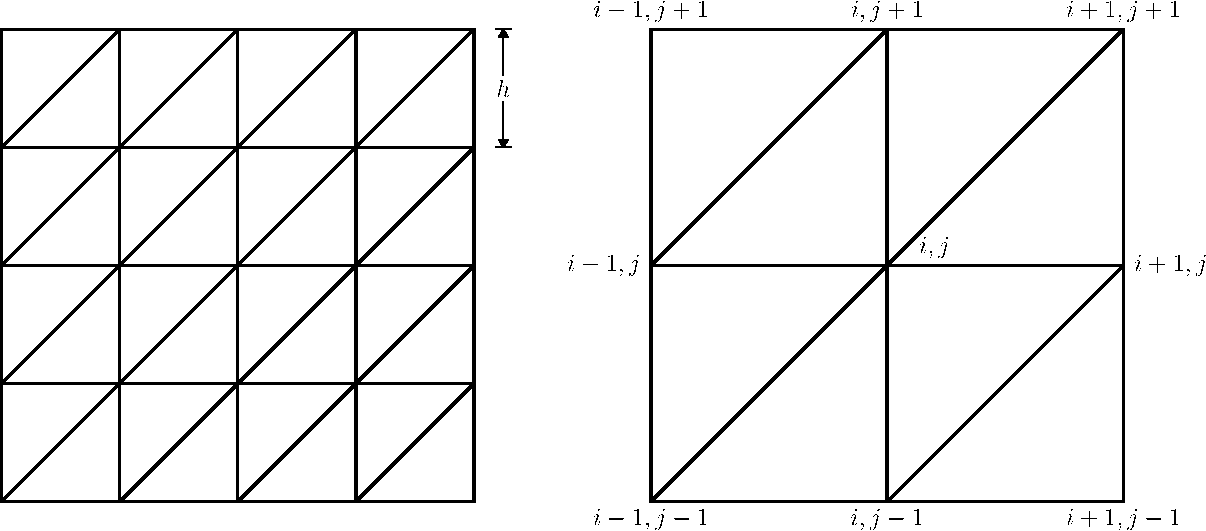
\includegraphics[height=1.5in]{figures/556uniform-grid}\hfill   
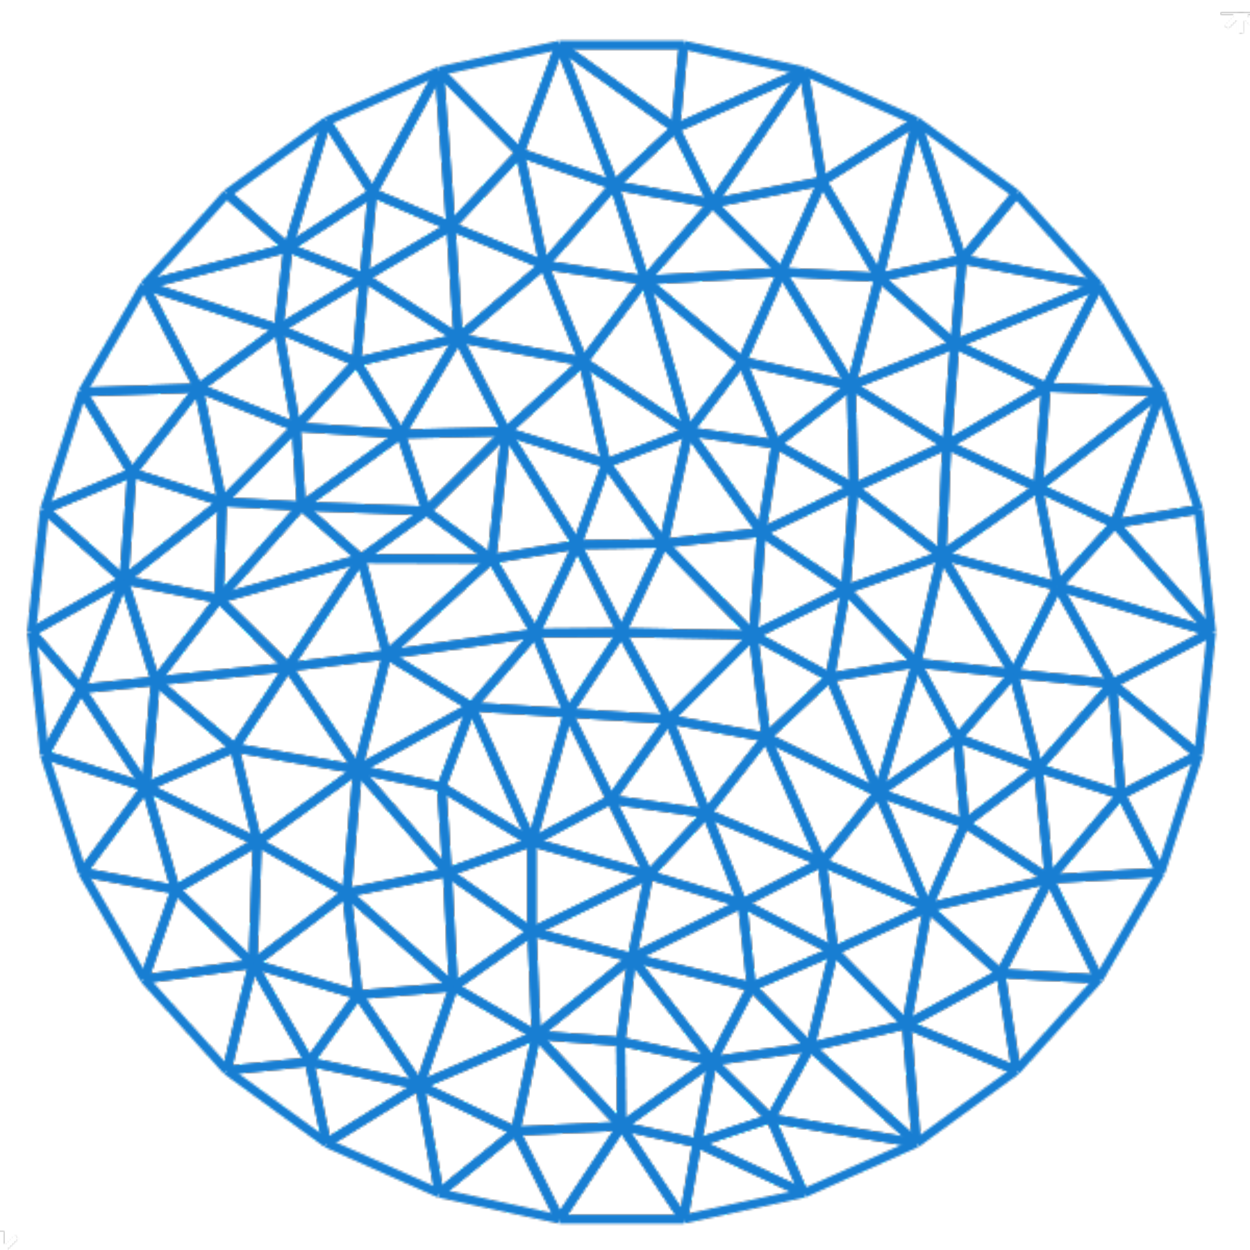
\includegraphics[height=1.5in]{figures/2ddiskpartition}
\caption{单位正方形的规则(均匀)三角剖分(左和中)和近似单位圆盘的非结构化网格(右)。   \label{fig:2dpartition}     }
\end{center}
\end{figure}     

我们使用拉普拉斯算子的标准中心差分近似
   \[
(-\Delta u)(x_i,y_j) \approx   
\frac{4u_{i,j}-u_{i+1,j}-u_{i-1,j}-u_{i,j+1}-u_{i,j-1}}{h^2}.
\]    然后,有限差分方案由
   \begin{equation}
  \label{2d-fd0}
4u_{i,j}-(u_{i+1,j}+u_{i-1,j}+u_{i,j+1}+u_{i,j-1})=h^2f_{i,j},
\end{equation}    给出,其中
   \begin{equation}
  \label{fij-fd}
f_{i,j} = f(x_i, y_j) 
\end{equation}    和    $u_{i,j} \approx u(x_i,y_j)$    。近似值    $u_{i,j}$    是通过求解线性系统找到的。我们按字典顺序对点    $(x_i,y_j)$    进行排序,对于    $k=1, \dots, n^2$    ,我们有
   \begin{equation}
  \label{lexi}
k=(j-1)n+i,  \quad x^h_{k}=(x_i,y_j), \quad \mu_k=u_{i,j},\quad 1\le i,j\le n, 
\end{equation}     

然后,我们可以将    \eqref{2d-fd0}    写为
   \begin{equation}\label{2d-fd}
A\mu=b,
\end{equation}    其中
   \begin{equation}
  \label{iso-A}
A=\operatorname{tridiag} (-I, B, -I), \mbox{ and }
B=\operatorname{tridiag} (-1, 4, -1). 
\end{equation}    使用更多    $(x_i, y_j)$    的相邻点可获得略有不同的方案。我们可以使用 8 个点    $(x_{i\pm 1}, y_{j\pm 1})$    和“中心”点    $(x_i, y_j)$    构建近似值。结果,我们得到如下 9 点有限差分方案:
   \begin{eqnarray}
 &&   8\mu_{i,j} - \mu_{i-1, j}-\mu_{i+1, j}-\mu_{i, j-1}-\mu_{i, j+1}
    \label{2d-fd-9p}  \\  \label{9-point}
&&\phantom{8\mu_{i,j}} - \mu_{i-1, j-1} -\mu_{i+1, j-1}-\mu_{i-1, j+1}-\mu_{i+1,j+1}=2h^2f_{i,j}. 
\nonumber
\end{eqnarray}    同样,如果我们按字典顺序排列    $(x_i, y_j)$   ,则~    \eqref{2d-fd-9p}    是线性系统~    \eqref{2d-fd}   ,对应于拉普拉斯方程的 9 点有限差分离散化,其中
   \begin{equation}
  \label{9point}
A=\operatorname{tridiag}(-C, B, -C) \mbox{ with }
B=\operatorname{tridiag}(-1, 8,-1), C=\operatorname{tridiag}(1, 1,1).
\end{equation}     

现在我们给出一个有限元离散化的例子。给定    $\Omega$    的三角剖分    ${\mathcal T}_h$   ,如图~    \ref{fig:2dpartition}    所示,让    $V_h\subset V$    成为由关于三角剖分    ${\mathcal T}_h$    的分段线性(或高阶)多项式组成的有限元空间。变分问题    \eqref{Vari}    的有限元近似为:找到    $u_h\in V_h$    使得
   \begin{equation}
  \label{vph}
a(u_h,  v_h)=(f,v_h), \quad\forall\,v_h\in V_h.
\end{equation}    假设    $ \{ \phi_i \} _{i=1}^{N}$    是    $V_h$    的节点基,即
对于任何节点    $x_j$    都有    $\phi_i(x_j)=\delta_{ij}$   。我们写出
   \(
        u_h(x)=\sum_{j=1}^{N}\mu_j\phi_j(x)
\)    方程    \eqref{vph}    等价于
   \[
        \sum_{j=1}^{N}\mu_ja(\phi_j,\phi_i)=(f,\phi_i),\quad
        j=1,2,\cdots, N, 
\]    ,它是一个线性方程组:
   \begin{equation}\label{axb}
        A\mu=b, \quad (A)_{ij} = a(\phi_j,\phi_i), \quad 
 \mbox{and}\quad (b)_i=(f,\phi_i).
\end{equation}    这里,矩阵    $A$    被称为节点基础的刚度矩阵
   $ \{ \phi_i   \} _{i=1}^N$    。  

对于    $d=2$    和图    \ref{fig:2dpartition}    所示的特殊均匀三角剖分,拉普拉斯算子的刚度矩阵恰好是    \eqref{2d-fd0}    给出的矩阵。这个特殊情况是有限差分和有限元方法之间密切关系的一个例子。  

我们注意到有限元方法基于变分公式    \eqref{Vari}    ,而有限差分方法则不是。然而,在 AMG 方法的开发中,变分方法也用于推导有限差分方法的粗水平方程。  

对于任何    $T\in \mathcal T_h$    ,我们定义
   \begin{equation}\label{hT}
        \overline h_T=\diam(T),\quad h_T=|T|^{\frac{1}{d}}, \quad \underline h_T=2\sup \{ r>0: B(x, r)\subset T \text{ for } x\in T \} .
    \end{equation}    如果存在一个均匀有界常数    $\sigma \ge 1$    使得 
   \begin{equation}
        \underline h_T\le h_T \le \overline h_T\le \sigma \underline h_T, \quad \forall T\in \mathcal T_h.
    \end{equation}    ,则我们称网格    $\mathcal T_h$    是形状规则的,并且我们称    $\sigma$    为形状规则性常数。  

假设    $h=\max_{T\in \mathcal T_h} \overline h_T$    ,其中    $\overline
    h_T$    定义在    \eqref{hT}    中。如果存在一个均匀有界常数
   $C > 0$    ,使得
   \begin{equation}
        \frac{h}{\underline h_T} \le C.
    \end{equation}    ,则我们称网格    $\mathcal T_h$    为准均匀网格  


 
 
 
   

   \subsection{光谱特性  }       \label{s:algebraic-spectral}    现在我们讨论    \eqref{Model0}    中给出的偏微分算子    ${\cal L}$    的谱特性。  

我们回顾一下著名的 Courant-Fischer 最小最大原理~    \cite{courant1924methoden}   ,它是对称矩阵的特征值。
   \begin{theorem}   \label{thm:minmax}    假设    $T$    是相对于    $(\cdot, \cdot)_*$    的    $n\times n$    对称矩阵,   $ \{ \lambda_j, \zeta_j \} $    是其与    $\lambda_1\le \lambda_2\le \cdots \le \lambda_n$    的特征对,则 
   \begin{equation}\label{minmax}
        \lambda_k=\min_{\dim W=k}\max_{x\in W, x\ne 0}\frac{(Tx, x)_*}{(x, x)_*},
    \end{equation}    中若 
   \begin{equation}\label{minmax-opt}
        W=\operatorname{span} \{ \zeta_j: j=1:k \} ,
    \end{equation}    则可达到最小值,而 
   \begin{equation}\label{maxmin}
        \lambda_k=\max_{\dim W=n-k+1}\min_{x\in W, x\ne 0}\frac{(Tx, x)_*}{(x, x)_*},
    \end{equation}    中若 
   \begin{equation}\label{maxmin-opt}
        W=\operatorname{span} \{ \zeta_j: j=k:n \} .
    \end{equation}    则可达到最大值  \end{theorem}    接下来,我们回顾一下    \cite{fan1949theorem}    中的定理 1,即 Ky-Fan 迹最小化原理。
   \begin{theorem}   \label{thm:fan}    假设    $T$    相对于    $(\cdot, \cdot)_*$    对称,且
   $ \{ \lambda_j, \zeta_j \} $    是其与
   $\lambda_1\le \lambda_2\le \cdots \le \lambda_n$    的特征对,则
   \begin{equation*}
        \min_{P\in \mathbb{R}^{n\times k}, P^*P=I}\operatorname{trace}(P^*TP) = \sum_{j=1}^{k}\lambda_j.
    \end{equation*}    此外,当 
   \begin{equation*}
    \operatorname{range}(P)=\operatorname{span} \{ \zeta_j \} _{j=1}^{k} \text{ and } P^*P=I. 
\end{equation*}    时可达到最小值 这里    $P^*\in \mathbb{R}^{k\times n}$    是    $P$    的伴随项,对应于    $(\cdot, \cdot)_*$    的内积,即
   \begin{equation*}
        (P^* u, v)= (u, Pv)_*, \quad \text{for all } u\in \mathbb{R}^{n}, v\in \mathbb{R}^{k}.
    \end{equation*}     \end{theorem}     

最后,在    \cite{1992XuJ-aa}    之后,我们使用符号
   $a\lesssim b$    来表示通用正常数    $C$    的存在,该数与问题大小、各向异性比率等重要参数无关,并且    $a\le Cb$    。此外,当且仅当    $a\lesssim b$    和
   $b\lesssim a$    时,我们才写出    $a\eqqsim b$    。  

   \begin{theorem}PDE 算子    ${\mathcal L}$    具有一组完整的特征函数
   $(\varphi_k)$    和非负特征值 
   $$
0\le\lambda_1\le\lambda_2\le \ldots 
$$    ,使得 
   $$
{\mathcal L}\varphi_k=\lambda_k\varphi_k, \quad k=1, 2, 3\ldots. 
$$    
   \begin{enumerate}

   \item            $\lim_{k\to\infty}\lambda_k=\infty.$            \item            $(\varphi_i)$          构成          $V$          以及          $L^2(\Omega)$          的正交基。  \end{enumerate}    此外
   \begin{enumerate}

   \item   对于纯诺伊曼问题,         $\lambda_1=0$          和          $\varphi_1$          是常数函数。   \item   对于纯狄利克雷问题,         $\lambda_1>0$          很简单,而          $\varphi_1$          不会改变符号。  \end{enumerate}     \end{theorem}     

我们有著名的 Weyl 对拉普拉斯算子的渐近行为的估计
   \cite{weyl1911asymptotische,wbyii1912asymptotische,reed1978iv}    。
   \begin{lemma}[Weyl's law]   \label{lem:Weyl}    假设    $\Omega$    满足(这意味着    $\Omega$    可以通过    $\mathbb{R}^d$    中的立方体并集来近似,有关确切定义,请参阅    \cite[page
  271]{reed1978iv}   )。对于均匀狄利克雷边界条件,纯拉普拉斯算子的特征值满足:
   \begin{equation}\label{Weyl0}
    \lim_{k\rightarrow\infty}\frac{\lambda_k}{k^{\frac{2}{d}}}=w_{\Omega},
    \mbox{ with }
    \quad w_{\Omega}=\frac{(2\pi)^2}{[\omega_d \operatorname{Vol}(\Omega)]^{\frac{2}{d}}},
\end{equation}    其中    $\omega_d$    是    $\mathbb{R}^d$    中单位球的体积,而    \eqref{Model0}    中给出的算子    $\mathcal L$    的特征值满足:
   \begin{equation}\label{Weyl}
    \lambda_k\eqqsim k^{\frac{2}{d}}, \quad \forall k\ge 1.
\end{equation}     \end{lemma}     

接下来,我们将上述韦尔定律扩展到离散化的 PDE 算子。以下定理给出了有限元离散化的韦尔定律的离散版本。有关此类结果的更多详细信息,请参阅~    \cite{Weyl}    。  

   \begin{theorem}   \label{thm:WeylFE}    假设    $V_h\subset H_0^1({\Omega})$    是具有    $\dim V_h = N$    的准均匀网格上的有限元空间族。考虑    \eqref{Model0}    
   \begin{equation*}
    \mathcal L_h: V_h\mapsto V_h, \quad (\mathcal L_h u, v) = a(u, v), \quad \forall u, v\in V_h,
\end{equation*}    的离散化算子及其特征值:
   \[
\lambda_{h,1}\le \lambda_{h,2}\le \cdots \lambda_{h,N}.
\]    然后,对于所有
   $1\le k\le N$    ,存在一个独立于    $k$    的常数    $C_w>0$    ,因此我们有以下估计值:
   \begin{equation}\label{e:discrete-continuous}
        \lambda_k\le\lambda_{h,k}\le C_w\lambda_k.
    \end{equation}    和 
   \begin{equation}\label{discrete-Weyl}
        \lambda_{h,k}\eqqsim k^{2/d}.
    \end{equation}     \end{theorem}     

   \subsection{有限元矩阵的性质  }       \eqref{axb}    给出的刚度矩阵的主要代数性质为:它是稀疏的,具有    ${\cal O}(N)$    非零值,是对称正定的(对于狄利克雷和混合边界条件都是如此),并且对于纯诺伊曼边界条件是半正定的;其特征值满足离散韦尔定律。  

为简单起见,本节的其余部分我们将仅考虑纯狄利克雷边界条件。
   \begin{lemma}   \label{lm:stiffness}       \eqref{axb}    给出的刚度矩阵    $A$    具有以下属性:
   \begin{enumerate}

   \item            $A$          的条件数由          $A$          的极值特征值之比定义,
         $$
\kappa(A)=\frac{\lambda_{\max}(A)}{\lambda_{\min}(A)},
$$          满足
         $$
\kappa(A) \eqqsim h^{-2}.
$$          此外,
         $$
\lambda_{\min}(A) \eqqsim h^2 \mbox{ and } \lambda_{\max}(A)\eqqsim 1.
$$            \item   韦尔定律的离散版本成立:
         $$
        \lambda_k(A)\eqqsim \left(\frac{k}{N}\right)^{2/d}.
$$           \end{enumerate}     \end{lemma}     

接下来,我们讨论    $d=2$    的单位平方域    $\Omega=(0, 1)\times (0, 1)$    的均匀网格有限元刚度矩阵的一些更精细的谱特性。我们从泊松方程开始。很容易推导出由    \eqref{2d-fd}    给出的    $A$    特征对的闭式解,我们有:
   \begin{equation}
  \label{2d-stiffness-eigenvalue}
\lambda_{kl}(A)
=4\left(\sin^2{{k\pi}\over {2(n+1)}}+\sin^2{{l\pi}\over {2(n+1)}}\right),
\end{equation}    和 
   \begin{equation}
\label{2d-stiffness-eigenvector}
\phi^{kl}_{ij}=\sin\frac{ki\pi}{n+1}\sin\frac{lj\pi}{n+1}, \quad 1\leq i\leq n, \quad 1\leq j\leq n.
\end{equation}     

现在考虑各向异性问题    \eqref{eq:anisotropic}    的重要情况。我们按字典顺序排列三角剖分的顶点,并像以前一样用    $ \{ (ih,jh) \} _{i,j=0}^n$    表示它们。刚度矩阵为
   \begin{equation}
  \label{aniso-A}
	A=\operatorname{tridiag} (-I, B, -I)\quad\mbox{with}\quad
 B=\operatorname{tridiag} (-\epsilon, 2(1+\epsilon), -\epsilon).
\end{equation}    显然,
   $$
	A=I\otimes B+C\otimes I\quad\mbox{with}\quad C=\operatorname{tridiag}(-1,0,-1),
$$    并且很容易验证
   $$
\lambda_i(B)=2(1+\epsilon)-2\epsilon\cos{{i\pi}\over {(n+1)}}, \quad
\lambda_j(C)=-2\cos{{j\pi}\over {(n+1)}},\quad 1\leq i,j\leq N.
$$    这导致特征值的以下表达式
   $$
\lambda_{ij}(A)
=4\epsilon\sin^2{{i\pi}\over {2(n+1)}}+4\sin^2{{j\pi}\over {2(n+1)}}.
$$    和相应的特征向量
   $$
\phi_{ij}^{k\ell}=\sin{{ki\pi}\over {n+1}}\sin{{\ell j\pi}\over {n+1}}.
$$     

   \section{线性向量空间和对偶  }       \label{s:duals}    在本文中,我们将主要考虑以下形式的线性方程组:
   \begin{equation}
  \label{auf}
Au=f.  
\end{equation}    这里 
   \begin{equation}
A: V\mapsto V',  
\end{equation}    
   $$
 \quad f\in V',
$$    
   $V$    是有限维线性向量空间,   $V'$    是    $V$    的对偶。如果我们使用符号    $\langle\cdot, \cdot\rangle$    表示    $V'$    和    $V$    之间的配对,我们可以将    \eqref{auf}    写成变分形式:找到    $u\in V$    使得
   \begin{equation}
  \label{VariAu=f}
a(u,v)=\langle f, v\rangle, \quad\forall v\in V 
\end{equation}    其中
   \begin{equation}
a(u,v)=\langle Au, v\rangle.  
\end{equation}     

   \subsection{对偶和内积  }    为方便说明,我们假设    $V$    具有内积    $(\cdot, \cdot)$    。根据 Riesz 表示定理,对于任何    $f\in V'$    ,都有唯一的    $u\in V$    使得
   \begin{equation}
  \label{L2dual}
(u,v) = \langle f, v\rangle, \quad \forall v\in V.   
\end{equation}    通过这种表示,我们将取    $V'=V$    。在本文的其余部分,为方便起见,对于任何有限维向量空间    $V$    ,我们始终假设    $V'=V$    。结果,我们有
   \begin{equation}
  \label{dualdual}
V''=(V')'=V'=V.  
\end{equation}    由于通过    \eqref{L2dual}    识别了    $V'=V$    ,   \eqref{dualdual}    中的身份非常明确,没有任何歧义。  

我们想指出的是,在对问题    \eqref{auf}    的所有迭代方法进行抽象讨论时,使用抽象对偶配对    $\langle\cdot, \cdot \rangle$    就足够了,而不必在    $V$    上引入内积    $(\cdot, \cdot)$   。但我们发现使用内积便于阐述,这一点我们稍后会看到。我们进一步指出,在本文中,我们不会使用内积来识别任何无限维向量空间的    $V'=V$   。  

如果    $ \{ \phi_i \} _{i=1}^N$    是    $V$    的一个基,我们总是会选择    $V'$    的一个基,即    $ \{ \psi_i \} _{i=1}^N$    ,它是    $V$    基的对偶。即    \begin{equation}
  \label{dual-basis}
(\psi_j, \phi_i)=\delta_{ij}, \quad 1\le i, j\le N.   
\end{equation}    这样的对偶基仅用于理论考虑,不会在任何算法的实际实现中使用。  

我们只考虑两种线性向量空间:第一种是    $V=\mathbb R^n$    ,内积就是点积
   $$
(u, v)_{\ell^2}=\sum_{i=1}^nu_iv_i, \quad \forall u=(u_i), v=(v_i)\in \mathbb R^n, 
$$    ,    $\mathbb R^N$    的标准基由单位矩阵的列向量组成,    $ \{ e_i \} _{i=1}^N$    ,很容易看出它的对偶基    $(\mathbb R^N)'=\mathbb R^N$    就是原始基
   $ \{ e_i \} _{i=1}^N$    本身。  

第二种是    $L^2(\Omega)$    对于给定域    $\Omega\subset\mathbb R^d$    (    $1\le d\le 3$    ) 的有限维函数子空间,配备    $L^2$    内积:
   $$
(u,v)=\int_\Omega u(x)v(x).
$$    一种常用的线性向量空间是有限元空间
   $V_h$    ,通常使用节点基函数    $ \{ \phi_i \} _{i=1}^N$    作为基。在这种情况下,   $V'$    的对偶基    $ \{ \psi_i \} _{i=1}^N$    不再是原始的节点基函数,而是一组满足
   \eqref{dual-basis}    的函数(通常全局支持)。这组对偶基函数通常在推导各种空间及其对偶之间的算子矩阵表示时需要,但在相关算法的实际实现中不需要它们。  

对于线性算子 
   \begin{equation}
  \label{LVV}
L: V\mapsto V,
\end{equation}    ,其伴随:
   \begin{equation}
  \label{Ldual}
L': V\mapsto V,
\end{equation}    定义如下
   \begin{equation}
  \label{LdualL}
(L'u,v)=(u, Lv),\quad u,v\in V.   
\end{equation}    由于    $V$    同时扮演    $V$    和其对偶    $V'$    的角色,因此概念
   \eqref{LVV}    和    \eqref{Ldual}    可以具有四种不同含义:
   \begin{enumerate}[1.]

   \item   如果    $L: V\mapsto V$    ,则    $L': V'\mapsto V'$    ;   \item   如果    $L: V\mapsto V'$    ,则    $L': V\mapsto V'$    ;   \item   如果    $L: V'\mapsto V$    ,则    $L': V'\mapsto V$    ;   \item   如果是    $L: V'\mapsto V'$    ,那么就是    $L': V\mapsto V$    。  \end{enumerate}    由于我们通过
   \eqref{L2dual}    对    $V'$    和    $V$    进行了识别,因此定义    \eqref{LdualL}    适用于上述所有四种不同情况。  

如果    $V=\mathbb R^n$    和    $(u,v)=(u,v)_{\ell^2}$    ,    $L' = L^T$    ,即矩阵转置。我们称算子    $A:V\mapsto V'$    是对称正定的 (SPD),如果 
   $$
A'=A, \quad (Av,v)>0\quad \forall v\in V\setminus \{ 0 \} .
$$     

当    $A$    为 SPD 时,它在    $V$    上定义了另一个内积    $(\cdot, \cdot)_A$    :
   $$
(u,v)_A=(Au,v),\quad u,v\in V
$$    和相应的范数 
   $$
\|v\|_A=(v,v)_A^{1/2}, \quad v\in V. 
$$    我们使用上标 ``*'' 表示关于    $\innerA$    的伴随算子,即 
   $$
(Bu, v)_A = (u, B^*v)_A. 
$$    很容易看出 
   \begin{equation}
  \label{BA}
 (BA)^* = B'A,
\end{equation}    和    $(BA)^* = BA$    当且仅当    $B'=B$    。  

   \subsection{矩阵表示  }    让    $V_c\subset V$    成为子空间并考虑包含算子    $\imath_c:
V_c\mapsto V$    。假设    $ \{ \phi_i^c \} _{i=1}^{n_c}$    和    $ \{ \phi_i \} _{i=1}^n$    分别是    $V_c$    和    $V$    的基函数,   $\imath_c$    的矩阵表示是矩阵 
   \begin{equation}\label{defP}
P:\mathbb R^{n_c}\mapsto \mathbb R^n \mbox{ satisfying }
(\phi_1^c,\ldots, \phi_{n_c}^c)=(\phi_1,\ldots, \phi_n)P. 
\end{equation}    上面写的恒等式是通过    $V$    中的基础扩展    $V_c$    中的基础的简写:
   \begin{equation}\label{Pexpand}
\phi_k^c =\sum_{j=1}^n p_{jk} \phi_j, \quad \quad P=(p_{jk}),\quad k=1,\ldots, n_c, \quad j=1,\ldots,n.
\end{equation}       $\imath_c': V'\mapsto V_c'$    的矩阵表示是什么?虽然我们有    $V'=V$    和    $V_c'=V_c$    ,但我们需要分别使用对偶基 
   $ \{ \psi_i^c \} _{i=1}^{n_c}\subset V_c'$    和    $ \{ \psi_i \} _{i=1}^n\subset V'$    。对于这些对偶基,   $\imath_c'$    的矩阵表示就是    $P^T$   (   $P$    的转置),因为很容易验证
   $$
(\imath_c'\psi_1,\ldots, \imath_c'\psi_n)=(\psi_1^c,\ldots, \psi_{n_c}^c)P^T.
$$     

现在考虑一个线性算子 
   \begin{equation}
  \label{AVV}
A:V\mapsto V.
\end{equation}    有两种不同的方法来获得    $A$    的矩阵表示,因为    $V$    在这里扮演两个角色。首先    $V$    是    $V$    本身,其次是    $V=V'$    。对于第一种情况,我们使用与    $V$    相同的基础    $ \{ \phi_i \} $    作为    $A$    的定义域,使用    $V$    作为    $A$    的范围。在这种情况下,   $A$    的矩阵表示是矩阵 
   \begin{equation}
  \label{matrixrep0}
\hat A\in \mathbb R^{n\times n}\mbox{ satisfying }
(A\phi_1, \ldots, A\phi_n)  =(\phi_1, \ldots, \phi_n)\hat A. 
\end{equation}    在第二种情况下,我们使用    $V$    的基础    $ \{ \phi_i \} $    作为    $A$    的定义域空间,但使用    $V'=V$    的对偶基础    $ \{ \psi_i \} $    作为    $A$    的范围空间。在这种情况下,   $A$    的矩阵表示为矩阵 
   \begin{equation}
\label{matrixrep}
\tilde A\in \mathbb R^{n\times n}\mbox{ satisfying }
(A\phi_1, \ldots, A\phi_n)  =(\psi_1, \ldots, \psi_n)\tilde A. 
\end{equation}    很容易看出
   \begin{equation}
  \label{tildeA}
\tilde A=\bigg((A\phi_j,\phi_i)  \bigg)
\end{equation}    和
   \begin{equation}
  \label{hatA}
\tilde A=M\hat A, \quad M=\bigg((\phi_j,\phi_i)  \bigg).
\end{equation}       \eqref{tildeA}    中的矩阵    $\tilde A$    通常被称为    $A$    的刚度矩阵,而    \eqref{hatA}    中的矩阵    $M$    被称为质量矩阵。  

在早期的多重网格文献中,通常会为有限元空间引入与    $L^2$    内积等价的离散内积,以便相应的质量矩阵变为对角矩阵。但如果我们以略微不同的方式查看底层有限元算子(如    \eqref{AVV}    中所示):
   \begin{equation}
  \label{AVVdual}
A: V\mapsto V',  
\end{equation}   ,我们就会很容易地看到,引入离散
   $L^2$    内积是不必要的。  

如果    $V=\mathbb R^n$    并且我们为    $V$    选择规范基    $ \{ e_i \} $    ,我们就不会遇到函数空间情况下的质量矩阵问题,因为在这种情况下    $ \{ e_i \} $    也是    $V'$    的对偶基。这当然很方便,但这种方便往往会隐藏给定问题中各种向量和矩阵与它们所表示的对象(函数)之间的一些微妙但重要的差异。  

给定一个矩阵    $A\in \mathbb R^{n\times n}$    ,我们可以将其视为
   \begin{equation}
  \label{A0}
A: \mathbb R^{n}\mapsto \mathbb R^{n},
\end{equation}    或
   \begin{equation}
  \label{A1}
A: \mathbb R^{n}\mapsto (\mathbb R^{n})'.  
\end{equation}    事实证明,当    $A$    由偏微分方程的离散化获得时,   \eqref{A1}    比
   \eqref{A0}    更具信息量。因此我们写一个矩阵方程
   \begin{equation}
  \label{Axb}
Ax=b  
\end{equation}    有时候将    $x$    和    $b$    视为两个“不同”的空间会很有帮助:
   \begin{equation}
  \label{xb}
x\in   \mathbb R^{n} \mbox{ and } b\in (\mathbb R^{n})'.  
\end{equation}     

   \subsection{特征值和特征向量  }    让我们简单讨论一下对称算子    $T: V\mapsto V$    的特征值和特征向量。如果    $(\lambda, \phi)$    是    $T$    的特征对,
   $$
T\phi=\lambda \phi.
$$    那么很容易看出    $(\lambda, \tilde\phi)$    是    $T$    的矩阵表示    $\tilde T$    的特征对:
   $$
\tilde T\tilde\phi=\lambda\tilde \phi. 
$$    这里    $\tilde\phi=\in \mathbb R^n$    是    $\phi$    的向量表示:
   $$
\phi=(\phi_1, \ldots,\phi_n)\tilde\phi.
$$    我们注意到,对于在    \eqref{AVV}    中定义的算子    $A$    ,我们在谈论    $A$    的特征值时需要谨慎。虽然我们通过    \eqref{L2dual}    来标识
   $V'=V$    ,但    $V'$    和    $V$    扮演着两个不同的角色,因此    $A$    本质上是两个“不同”空间
   $V$    和    $V'$    之间的映射,而    $A$    的频谱应该仔细定义。但如果我们考虑对称运算符
   \begin{equation}
  \label{RVV}
R: V'\mapsto V.  
\end{equation}    ,则    $RA: V\mapsto V$    是一个关于
   $A$    -内积对称的运算符。在这种情况下,如果    $(\lambda, \phi)$    是    $RA$    的特征对,则    $(\lambda, \tilde \phi)$    是    $\tilde
R\tilde A$    的特征对(等于    $RA$    的矩阵表示)  

如果我们考虑一个平凡的识别算子 
   $$
\jmath:  V'\mapsto V \mbox{ such that } \jmath
\psi_i=\psi_i,\quad\forall i.
$$    即对所有    $v\in V'=V$    的    $\jmath v=v$    。很容易看出    $\jmath$    的矩阵表示是质量矩阵的逆
   $M=((\phi_j,\phi_i))$    ,即
   $$
\tilde \jmath=M^{-1}.
$$    使用此识别算子,算子    $\jmath A: V\mapsto
V$    是从    $V$    到    $V$    的对称算子。然后我们可以讨论它的谱。例如,如果    $(\lambda, \phi)$    是    $\jmath A$    的特征对,则    $(\lambda, \tilde\phi)$    满足
   $$
\tilde A\tilde \phi=\lambda M\tilde \phi.
$$    这通常是有限元分析中出现的广义特征值问题。  

尽管对于所有的    $v\in V$    、    $\jmath Av=Av$    来说,由于上面介绍的标识,    $\jmath A$    和    $A$    严格来说是两个不同的运算符:它们有两个不同的范围,并且它们的矩阵表示也不同。  

上述讨论虽然简单,但乍一看可能有点令人困惑,但明确理解和澄清这些概念及其背后的微妙之处将有助于本文其余部分介绍代数多重网格方法。有关相关主题的更详细讨论,请参阅    \cite{XuMSC-Notes}    。  

   \subsection{书目注释  }    有关此处使用的基本线性代数材料的一般阅读,请参阅~    \cite{1974HalmosP-aa,1992XuJ-aa,XuMSC-Notes}    。具体而言,有关对偶空间和矩阵表示的更详细讨论,请参阅~    \cite{1992XuJ-aa,XuMSC-Notes}    。  

   \section{基本迭代方法  }    
   \label{sec:iterate}    现在我们考虑用于解决    \eqref{axb}    的线性迭代方法。我们将重点介绍两种最常用的算法,即雅可比和高斯-赛德尔方法。让我们首先在更一般的环境中简要介绍一下线性迭代方法。回想一下正在考虑的基本问题:给定一个有限维向量空间    $V$    ,其配备内积
   $(\cdot,\cdot)$    ,我们考虑
   \begin{equation}
\label{Auf}
Au=f,   
\end{equation}    ,其中    $ A: V\mapsto V' $    是对称正定 (SPD) ,   $V'$    是    $V$    的对偶。如在    \S       \ref{s:duals}    中提到的,我们将通过内积    $(\cdot, \cdot)$    识别    $V'=V$    。  

   \subsection{基本迭代方法  }    解决    \eqref{Auf}    的一般线性迭代方法可以写如下:给定    $u^0\in V$    ,
   \begin{equation}
\label{eq:iterate}
u^{m}= u^{m-1}+B(f-Au^{m-1}), \quad m=1,2,\cdots ,
\end{equation}    其中    $B: V'\mapsto V$    是线性算子,可以被认为是    $A$    的近似逆。  

有时迭代器    $B$    是对称的更为可取。如果
   $B$    不对称,则有一种自然的方法可以使其对称。考虑以下迭代
   \begin{equation}
\label{symmetrized-iteration}  
\left \{ 
\begin{array}{lcl}
u^{m-1/2} &=& u^{m-1}+ B(f-Au^{m-1}), \\ 
u^{m} &=& u^{m-1/2}+ B'(f-Au^{m-1/2}).
\end{array}
\right.
\end{equation}    对称化迭代    \eqref{symmetrized-iteration}    可以写成
   \begin{equation}
\label{sym-iterate}
u^{m}= u^{m-1}+\bar B(f-Au^{m-1}), \quad m=1,2,\cdots 
\end{equation}    其中
   \begin{equation}\label{symm}
\bar B=B'+B-B'AB,
\end{equation}    满足
   \begin{equation}\label{symm1}
I-\bar BA=(I-BA)^*(I-BA).
\end{equation}    显然,    $\rho(I-\bar BA)<0$       $\Longleftrightarrow \bar B>0$    
   $\Longleftrightarrow$       $G\equiv (B')^{-1}+B^{-1}-A>0$    。  

   \begin{theorem}   \label{thm:iterate-converge}    以下结果成立
   \begin{enumerate}

   \item      \eqref{symmetrized-iteration}    收敛          $\Longleftrightarrow$          
         $G>0 \Longrightarrow $             \eqref{eq:iterate}    收敛。此外
   \begin{equation}
  \label{errA}
\|I-BA\|_A^2
=\lambda_{\max}(I-\bar BA)
=1-\left(\sup_{\|v\|_A=1}(\bar B^{-1}v,v)\right)^{-1}
\end{equation}      \item   如果          $B'=B$          、          $G>0 \Longleftrightarrow$          和    \eqref{eq:iterate}    收敛,并且          $\eta=\lambda_{\min}(G)$          、 
   \begin{equation}
  \label{BB}
  \frac{2\eta}{\eta+1}(Bv,v)\le (\bar Bv,v)\le
  2(Bv,v), \quad v\in V. 
\end{equation}     \end{enumerate}     \end{theorem}     

   \exercise    将定理    \ref{thm:iterate-converge}    推广到    $A$    为 SSPD 的情况。  

   \subsection{雅可比和高斯-赛德尔方法  }    对于
   $A=(a_{ij})\in\mathbb R^{n\times n}$    ,我们写为 
   $$
A=D+L+U,
$$    ,其中    $D$    是    $A$    的对角线,   $L$    和    $U$    分别是    $A$    的严格下三角和上三角部分。  

给定    $\omega>0$    ,(修改后的)雅可比方法可以写成
   \eqref{eq:iterate}    与 
   $$
B=\omega D^{-1}=(\omega^{-1} D)^{-1},
$$    ,得到的算法如下:  

   \begin{algorithm}   \caption{修正雅可比  }    
   $$
    \mbox{For } i=1:n,\quad
x_i^{m}=x_i^{m-1}+\omega a_{ii}^{-1}\left(b_i-\sum_{j=1}^{n}a_{ij}x_j^{m-1}\right).
$$     \end{algorithm}     

(改进的) 高斯-赛德尔方法可以写成
   \eqref{eq:iterate}    与 
   $$
B=(\omega^{-1} D+L)^{-1}
$$   ,得到的算法如下:  

   \begin{algorithm}   \caption{修正高斯-赛德尔法  }    
   \label{alg:modifiedGS}    
   $$\mbox{For } i=1:n,\quad 
    x_i^{m}= x_i^{m-1}+\omega a_{ii}^{-1}\left(b_i-\sum_{j=1}^{i-1}a_{ij}x_j^{m}
-\sum_{j=i}^{n}a_{ij}x_j^{m-1}\right).$$     \end{algorithm}     

以下结果很容易从定理
   \ref{thm:iterate-converge}    得出,并且众所周知。
   \begin{theorem}修正雅可比法收敛于且仅当 
   \begin{equation}
  \label{omega-J}
0<\omega<\frac{2}{\rho(D^{-1}A)},   
\end{equation}    ,修正高斯-赛德尔法收敛于且仅当 
   \begin{equation}
\label{omega-GS}
0<\omega<2.
\end{equation}     \end{theorem}    在实践中,通常很容易正确选择    $\omega$    来满足
   \eqref{omega-J}   ,从而保证改进的雅可比方法收敛。在本文的其余部分,我们可能始终假设选择了    $\omega$   。对于高斯-赛德尔方法,我们将始终选择    $\omega=1$   (最佳 SOR 通常不用于多重网格方法)。雅可比和高斯-赛德尔方法及其收敛理论可以直接扩展到块矩阵。  

   \subsection{子空间校正方法  }       \label{sec:msc}    我们考虑一系列空间    $V_{1},\ldots,V_{J}$    。这些空间(称为  {    \it    辅助空间   }  )不一定是    $V$    的子空间,但它们中的每一个都通过线性算子与原始空间    $V$    相关
   \begin{equation}
  \label{Pai-k}
\Pi_k: V_k\mapsto V.   
\end{equation}    我们最基本的假设是以下分解成立:
   \begin{equation}
  \label{aux-decomp}
V=\sum_{i=1}^J\Pi_iV_i. 
\end{equation}    这意味着对于任何    $v\in V$    ,都存在    $v_i\in V_i$   (可能不是唯一的),使得
   \begin{equation}
  \label{aux-decomp0}
v=\sum_{i=1}^J\Pi_iv_i.   
\end{equation}    此外,我们假设每个    $V_i$    都配备有能量内积
   $a_i(\cdot,\cdot)$    。我们定义
   $$
A_i:  V_i\mapsto V_i',
$$    为
   $$
(A_iu_i,v_i)=a_i(u_i,v_i), \quad u_i,v_i\in V_i. 
$$    让    $\Pi_i':  V'\mapsto V_i'$    成为    $\Pi_i$    的伴随:
   $$
(\Pi_i'f, v_i)=(f,\Pi_i v_i), \quad f\in V',  v_i\in V_i.
$$    让    $P_i=\Pi_i^*: V\mapsto V_i$    成为    $\Pi_i$    关于 A 内积的伴随:
   $$
(P_iu,v_i)_{A_i}=(u,\Pi_iv_i)_{A}, u\in V, v_i\in V_i.
$$     

以下恒等式成立
   \begin{equation}
  \label{PiAAP}
  \Pi_i'A=A_iP_i.
\end{equation}     

如果    $u$    是    \Rf{Auf}    的解,则根据    \eqref{PiAAP}    ,我们有
   \begin{equation}
\label{3.3a}A_iu_i=f_i,
\end{equation}    其中
   $$
u_i=P_iu, \quad f_i=\Pi_i'f.
$$    该等式可视为    \Rf{Auf}    对
   $V_i$    的限制。我们假设每个这样的    $A_i$    都有一个近似逆或预条件子:
   \begin{equation}
  \label{Ri}
R_i: V_i'\mapsto V_i.   
\end{equation}     

 {    \it   并行子空间校正   } (简称 PSC)方法是
   \eqref{eq:iterate}   ,   $B=B_{psc}$    由
   \begin{equation}
  \label{PSC}
B_{psc}=\sum_{i=1}^J\Pi_iR_i\Pi_i'.
\end{equation}    给出  

 {    \it    逐次子空间校正   } (简称SSC)方法定义如下:  

   \begin{algorithm}   \caption{连续子空间校正法  }       \label{alg:MSC}    给定    $u^0\in V$    ,对于任意    $m=1,2,\ldots$    ,
   \begin{enumerate}[1.]

    \item            $v\leftarrow u^{m-1}$            \item            $v\leftarrow v+\Pi_iR_i\Pi_i'(f-Av)$         ,         $i=1,2,\ldots J$         ,   \item            $u^m\leftarrow v$           \end{enumerate}     \end{algorithm}     

算法    \ref{alg:MSC}    等同于    \eqref{eq:iterate}   ,其中
   $B=B_{ssc}$    由
   \begin{equation}
  \label{ssc}
I-B_{ssc}A= (I-T_J)(I-T_{J-1})\ldots(I-T_1),
\end{equation}    给出,其中
   \begin{equation}
  \label{Ti}
T_i  =\Pi_iR_i\Pi_i'A =\Pi_iR_iA_iP_i.
\end{equation}     

   \begin{theorem}   \label{thm:add}    假设所有    $R_k$    都是 SPD。然后
   \begin{equation}\label{eq:add}
(B_{psc}^{-1} v,v)  = \min_{\sum_i \Pi_iv_i=v}\sum_{k=1}^J(R_k^{-1}v_k, v_k)
\end{equation}    具有由
   \begin{equation}
  v_k^*=R_k\Pi_k'B_{psc}^{-1}v.
\end{equation}    给出的唯一最小化器  \end{theorem}     

   \begin{theorem}   \label{thm:c0}    根据上述假设,以下恒等式成立:
   \begin{eqnarray}
  \label{identity}
\|I-B_{ssc}A\|_A^2 
&= &\|(I-T_J)(I-T_{J-1})\ldots(I-T_1)\|_A^2 \nonumber \\ 
&= &1-\frac{1}{1+c_0}\label{identity0} \\ 
&= &1-\frac{1}{c_1}\label{identity1}.
\end{eqnarray}    这里 
   $$
c_0=\sup_{\|v\|_A=1}c_0(v),  \quad
c_1=\sup_{\|v\|_A=1}c_1(v) =1+c_0,
$$    和    $w_i= (I-T_i^{-1})\Pi_iv_i + \sum_{j=i+1}^J \Pi_jv_j$    
   \begin{equation}\label{defc0}
c_0(v)=\inf_{\sum_i \Pi_iv_i = v}
\sum_{i=1}^J (T_i\overline{T}_i^{-1}T_i^*w_i,w_i)_A,
\end{equation}    和 
   \begin{equation}\label{defc1}
    c_1(v)=(\overline{B}_{ssc}^{-1} v,v) =\inf_{\sum_i \Pi_iv_i = v} (\overline{T}_i^{-1}(\overline{T}_iT_i^{-1}\Pi_iv_i+T_i^*w_i), (\overline{T}_iT_i^{-1}\Pi_iv_i+T_i^*w_i))_A.
\end{equation}    特别是,如果    $R_i=A_i^{-1}$    ,则 
   \begin{equation}\label{c0v} 
c_0(v)
    = \inf_{\sum_i \Pi_iv_i = v}\sum_{i=1}^J\|P_i\sum_{j=i+1}^J \Pi_jv_j\|_{A_i}^2,
\end{equation}    和
   \begin{equation}\label{eq:mult} 
c_1(v)
= \inf_{\sum_i \Pi_iv_i = v}\sum_{i=1}^J\|P_i\sum_{j=i}^J \Pi_jv_j\|_{A_i}^2.
\end{equation}     \end{theorem}    
   \begin{lemma}   \label{lem:psc-ssc}    如果    $R_k=A_k^{-1}$    对于所有    $k$    都是如此,并且    $V_k$    是    $V$    的子空间,则 
   \begin{equation}
  \label{eq:3}
\frac14 
({B_{psc}^{-1}}v,v)\le ({\bar B_{ssc}^{-1}}v, v)\le c^*
(B_{psc}^{-1}v,v), \quad
v\in V.  
\end{equation}    其中
   \[
c^*=\max_{1\le k \le M} [N(k)]^2
\mbox{ with } 
N(k) = \left \{ j\in  \{ 1,\ldots,J \}  \;\big|\; 
\;\mbox{and}\;V_j\cap V_k\neq \{ 0 \}  \right \} .
\]     \end{lemma}    
   \begin{proof}给定    $v=\sum_{i=1}^J v_i$    和    $v_i\in V_i$    。由此得出
   $$
\|v\|_A^2
=\sum_{k,j=1}^J(v_k,v_j)_A
=\sum_{k=1}^J(v_k,v_k)_A+2\sum_{j>k}^J(v_k,v_j)_A
=-\sum_{k=1}^J(v_k,v_k)_A+2\sum_{j\ge k}^J(v_k,v_j)_A.
$$    因此
   \begin{eqnarray*}
\sum_{k=1}^{J}\|v_k\|_A^2
&\le &
2\sum_{k=1}^{J}(v_k,\sum_{j = k}^J v_j)_A
  =    2\sum_{k=1}^{J}(v_k, P_k\sum_{j = k}^J v_j)_A \\ 
&\le&
2(\sum_{k=1}^{J}\|P_k\sum_{j = k}^J v_j\|_A^2)^{1/2}
(\sum_{k=1}^{J}\|v_k\|_A^2)^{1/2}.
  \end{eqnarray*}    因此
   $$
\sum_{k=1}^{J}\|v_k\|_A^2
\le 4\sum_{k=1}^{J}\|P_k\sum_{j = k}^J v_j\|_A^2.
$$    根据    \eqref{eq:add}    、    \eqref{eq:mult}    和    \eqref{defc1}    ,我们得到
   $$
(B_{psc}^{-1}v,v)\le 4c_1(v) =4(\bar B_{ssc}^{-1}v,v).
$$    上限也很容易得出。从    $\|P_k\|_A= 1$    和 Schwarz 不等式,我们得到
   \begin{eqnarray*}
\sum_{k=1}^{J}\|P_k\sum_{j = k}^J v_j\|_A^2
&=& 
\sum_{k=1}^{J}\|P_k\sum_{j \in N(k); j\ge k} v_j\|_A^2 \\ 
& \le & 
\sum_{k=1}^{J}\|\sum_{j \in N(k); j\ge k} v_j\|_A^2\le 
\sum_{k=1}^{J}N(k)\sum_{j \in N(k); j\ge k} \|v_j\|_A^2  \\ 
&\le& 
\sqrt{c^*} \sum_{k=1}^{J}\sum_{j \in N(k); j\ge k} \|v_j\|_A^2 
\le 
c^* \sum_{k=1}^{J}\|v_k\|_A^2. 
\end{eqnarray*}    证明的结论是取两边所有分解的最小值并应用~    \eqref{eq:mult}    。  \end{proof}     

   \begin{remark}我们想指出的是,   \eqref{eq:3}    中的估计适用于各向异性和跳跃系数问题,并且常数    $c^*$    仅取决于子空间之间重叠的“拓扑”,而不取决于其他成分和属性。  \end{remark}     

Jacobi 和 Gauss-Seidel 方法可以解释为基于分解的 PSC 和 SSC
   $$
\mathbb R^n=\sum_{i=1}^n{\rm span}  \{ e_i \}  
$$    具有精确子空间解,使得
   $$
B_{psc}=D^{-1}, \quad B_{ssc}=(D+L)^{-1}, \quad
\bar B_{ssc}=(D+U)^{-1}D (D+L)^{-1}. 
$$    根据定理    \ref{thm:c0}    
   $$
c_0=\sup_{\|v\|_A=1}(D^{-1}Uv, Uv), \quad
c_1=\sup_{\|v\|_A=1}(D^{-1}(D+U)v, (D+U)v). 
$$    根据引理    \ref{lem:psc-ssc}    
   \begin{equation}
  \label{J-GS}
{1\over 4} (Dv,v) \le (D^{-1}(D+U)v, (D+U)v)\le c_*(Dv,v),\quad v\in \mathbb R^n   
\end{equation}     

我们注意到
   $$
c_1=
\sup_{v\in V}\frac{(\bar B_{ssc}^{-1}v, v)}{\|v\|_A^2}
\le \sigma \sup_{v\in V}\frac{\|v\|_D^2}{\|v\|_A^2}
$$    其中
   \begin{equation}
  \label{sigma}
    \sigma = \sup_{v\in V} \frac{\|v\|_{\bar{B}_{ssc}^{-1}}^2}{(D v,v)},  
\end{equation}    在上面的介绍中,大多数结果都是针对 SPD 问题的。我们想指出的是,所有这些结果都可以扩展到更一般的一类问题:即对称半正定问题。当    $A$    是矩阵时,我们进一步假设    $A$    的所有对角线都非零,因此为正。当子空间校正方法用于更一般的对称半正定算子    $A$    时,我们进一步假设每个    $A_i$    都是 SPD。我们应该使用首字母缩略词 SSPD 来表示满足上述属性的矩阵或算子。  

   \subsection{书目注释  }    Xu    \cite{1992XuJ-aa}    基于
   \cite{1991BrambleJ_PasciakJ_WangJ_XuJ-ac,1991BrambleJ_PasciakJ_WangJ_XuJ-aa}    描述了通过空间分解进行子空间校正的一般概念。这是一个抽象的观点,涵盖了一大类迭代算法(如多重网格和域分解方法)的理论和实践。在过去的二十年里,人们投入了大量精力来研究与这些方法相关的理论和实践问题。在~    \cite{Xu.J;Zikatanov.L.2002a}    中可以找到希尔伯特空间中加法和乘法方法理论的一般结果,这些结果适用于许多情况。有关文献综述和基本结果,我们请读者参阅一些专著和综述文章:   \cite{1985HackbuschW-aa}   、   \cite{1993BrambleJ-aa}   、
   \cite{2008VassilevskiP-aa}   、   \cite{1989XuJ-aa,1997XuJ-aa}   、
   \cite{xu1998some}   、   \cite{1993YserentantH-aa}   、
   \cite{2005ToselliA_WidlundO-aa}   、   \cite{1995GriebelM_OswaldP-aa}   、
   \cite{1996SmithB_BjorstadP_GroppW-aa}   。对于经典迭代方法的详细研究,我们参考专著~   \cite{1971YoungD-aa}   、   \cite{1994HackbuschW-aa}   、
   \cite{2000VargaR-aa}   、   \cite{2003SaadY-aa}   。  

我们注意到,在本节中我们考虑了 SSPD 矩阵,并且根据
   \cite{2008LeeY_WuJ_XuJ_ZikatanovL-aa,2007LeeY_WuJ_XuJ_ZikatanovL-aa,2014Ayuso-de-DiosB_BrezziF_MariniL_XuJ_ZikatanovL-aa}    ,本节中的所有结果对于具有半范数的 SSPD 问题均有效。辅助空间方法和子空间校正方法之间的关系在~    \cite{2011ChenL-aa}    中绘制。在经典多重网格文献~    \cite{1stAMG,Brandt.A;McCormick.S;Ruge.J.1985a,Ruge.J;Stuben.K.1987a,Trottenberg.U;Oosterlee.C;Schuller.A.2001a}    中,代数平滑(低)频率和代数高频的概念起着重要作用。它们也有助于设计新的 AMG 方法。如收敛估计所示,对于给定的平滑器,理想的粗空间应该能够捕获或很好地近似松弛矩阵    $\bar R A$    或    $D^{-1}A$    的频谱的下端。这通常称为近零空间 
   \cite{2015TreisterE_YavnehI-aa,2011LaiJ_OlsonL-aa,2009XuJ-aa}    ,
   \cite{2006BrezinaM_FalgoutR_MacLachlanS_ManteuffelT_McCormickS_RugeJ-aa}    。  

   \section{抽象多重网格方法和二层理论  }       \label{s:2Level}    在本节中,我们将在抽象环境中介绍代数多重网格方法。代数多重网格的首字母缩略词“AMG”也可用于代表抽象多重网格。  

我们将重点讨论两级方法。从算法设计的角度来看,将两级扩展到多级是很简单:通过递归应用两级算法可以得到通用的多级 V 循环算法。但将两级收敛理论扩展到多级情况可能非常困难。  

我们将仅考虑    \S       \ref{sec:iterate}    中描述的 SSPD 问题。与大多数文献中所做的那样,AMG 的设计原理是在给定平滑器的情况下优化粗空间的选择。最常用的平滑器是高斯-赛德尔方法和(修改或缩放的)雅可比方法。由于这些平滑器作为迭代方法本身是定性收敛的,因此得到的 AMG 方法始终是定性收敛的。我们的 AMG 收敛理论的任务是确保这种收敛在数量上也是快速的。特别是,对于由偏微分方程离散化产生的系统,我们希望我们的 AMG 方法相对于问题的大小和/或来自底层 PDE 的一些关键参数均匀收敛。我们有时将这种收敛称为“一致收敛”或“一致收敛”。  

事实证明,我们通常能够为两级 AMG 建立这种一致收敛,但很少能将这种一致收敛结果扩展到多级情况。对于二阶椭圆边界值问题,几何多重网格方法的多层收敛非常容易理解。但是,不使用几何信息的 AMG 的严格多层收敛理论仍然是一个悬而未决的问题。  

在本节以及本文的其余部分,我们将主要关注 AMG 方法的两级收敛理论。  

   \subsection{两级方法  }     


   


 
 
 
 
 
 
   

   \newcommand{\pr}     { 磷   }   

两级方法通常由以下部分组成:
   \begin{enumerate}[1.]

   \item   更平滑的    $R: V'\mapsto V$   ;   \item   粗空间    $V_c$    ,它可能是也可能不是
   $V$    的子空间,但通过延伸运算符与    $V$    链接:
   $$
\pr:  V_c\mapsto V. 
$$      \item   粗空间求解器    $B_c: V_c'\mapsto V_c$    。  \end{enumerate}     

在下面的讨论中,我们需要以下内积
   \begin{equation}\label{eq:norm-star}
\Tscalar{u}{v} = (\overline{T}^{-1} u,v)_A=( \bar R^{-1}u,v), \quad \overline{T} = \overline{R} A,
\end{equation}    和伴随范数    $\Tnorm{\cdot}$    。这里我们回想一下,    $\bar R$    的定义类似于    \eqref{symm}    中的定义。  

我们始终假设    $\bar R$    是 SPD,因此更平滑的    $R$    始终是收敛的。此外,
   \begin{equation}
    \|v\|_A^2\le \|v\|_{\bar R^{-1}}^2.
\end{equation}     


   

   \eqref{Auf}    的限制是
   \begin{equation}
  \label{coarse:Au=f}
A_cu_c=f_c,   
\end{equation}    其中 
   $$
A_c=\pr'A\pr, \quad f_c=\pr'f. 
$$     

粗空间求解器    $B_c$    经常被选为精确求解器,即    $B_c=A_c^{-1}$    ,用于分析,但在多级设置中,
   $B_c$    是递归定义的,它是
   $A_c^{-1}$    的近似值。我们在选择
   $B_c$    时区分这两种不同情况:
   \begin{eqnarray}
&& \mbox{ exact  two level method if         $B_c=A_c^{-1}$        .}\label{eq:exact} \\  
&& \mbox{ inexact  two level method if         $B_c\neq A^{-1}_c$        }.  \label{eq:inexact}
\end{eqnarray}    在    $A$    是半正定的情况下,我们使用    $N$    表示    $A$    的核,并且我们始终假设    $N\subset V_c$    。设
   \begin{equation}
    W:=N^{\perp}, \text{ and } W_c:=V_c\cap W,
\end{equation}    其中正交性相对于
   $(\cdot,\cdot)_{\bar{R}^{-1}}$    内积来理解。令    $Q_1: V \mapsto W$    为    $(\cdot,\cdot)_{\bar{R}^{-1}}$    内积的正交投影
   \begin{equation}\label{e:q0}
(Q_1v, w)_{\bar{R}^{-1}} = (v,w)_{\bar{R}^{-1}}, \quad\mbox{for
  all}\quad v\in V, w\in W. 
\end{equation}    
   $A_c$    在    $V_c$    上是半正定的,但在    $W_c$    上可逆。我们用    $\hat A_c$    表示    $A_c$    对    $W_c$    的限制,并定义    $A_c$    
   \begin{equation}
    A_c^{\dag}: = Q_1'\hat A_c^{-1} Q_1.
\end{equation}    的伪逆。虽然符号有些滥用,但我们仍将使用    $A_c^{-1}$    表示
   $A_c$    的伪逆,即
   $$
A_c^{-1}=A_c^\dag.
$$   。在本文的其余部分,我们将对其他相关奇异算子和矩阵的伪逆使用类似的符号。  

我们选择根据算子    $B:
V'\mapsto V$    来定义 AMG 算法,该算子可以视为    $A$    的近似逆或预处理器。典型的两级 MG 方法如下。
   \begin{algorithm}[H]   \caption{两级 MG 方法  }       \label{alg:two-level}    给定    $g\in V'$   ,动作    $Bg$    通过以下三个步骤定义
   \begin{enumerate}

   \item   粗网格校正:         $w=\pr B_c \pr' g$         。   \item   后平滑:         $Bg:= w +R(g-Aw)$         。  \end{enumerate}     \end{algorithm}     

在本节的其余部分,我们采用    $B_c=A_c^{-1}$    。  

通常有两种不同的(且在数学上等价的)方法来选择    $V_c$    、    $V$    、    $P$    和    $R$    。第一种称为运算符版本,其为 
   $$
V_c\subset V. 
$$    在本例中为    $P=\imath_c$    其中 
   \begin{equation}
  \label{inclusion}
\imath_c: V_c\to V,
\end{equation}    是    $V_c$    自然包含于    $V$    中。在二阶椭圆边界值问题的有限元离散化应用中,    $V_c$    和    $V$    只是 
   $H^1(\Omega)$    的有限元子空间。这种符号便于分析。但这不是可直接用于实现的算法。  

第二个称为矩阵版本,其中
   $$
V_c=\mathbb R^{n_c} \mbox{ and } V=\mathbb R^n,
$$    和 
   \begin{equation}
  \label{prolong}
P: \mathbb R^{n_c} \mapsto \mathbb R^n,
\end{equation}    是延长矩阵。  

这两组不同的符号通过使用 
   $ \{ \phi_i^c \} _{i=1}^{n_c}\subset  V_c$    和    $ \{ \phi_i: \} _{i=1}^{n}\subset  V$    的基函数相关联。如前所述,
   \eqref{defP}    --    \eqref{Pexpand}    中给出的延长矩阵    $P$    只是    \eqref{inclusion}    中给出的
   $\imath_c$    的矩阵表示,我们有
   \begin{equation}
  \label{icP}
(\phi_i^c, \ldots, \phi_{n_c}^c)=(\phi_i, \ldots, \phi_n)P.
\end{equation}    以下观察很明显。
   \begin{observation}找到一个粗空间    $V_c\subset V$    相当于在    \eqref{prolong}    中找到一个延长矩阵    $P$    。  \end{observation}     

   \begin{lemma}两级 AMG 算子    $E=I-BA$    的误差传播算子为
   \begin{equation}\label{E_op}
        E=(I-RA)(I-\Pi_c), 
    \end{equation}    ,其中    $\Pi_c= \imath_cA_c^{-1}\imath_c'A$    是    $(\cdot,\cdot)_A$    在    $V_c$    上的正交投影,以矩阵表示为    $\Pi_c=PA_c^{-1}P^TA$    。  \end{lemma}     

   \subsection{最优两级 AMG 理论  }       \label{2-level-theory}    AMG 方法的设计是为了平衡平滑器
   $R$    和粗空间    $V_c$    之间的相互作用。大多数现有 AMG 的设计是首先固定一个平滑器,通常由雅可比或高斯-赛德尔方法(或它们的组合和变体)给出,然后优化粗空间的选择。这是我们在本文中主要讨论的方法。但我们也评论了一种不同的方法,即首先固定粗空间,然后尝试优化平滑器的选择。也可以尝试同时对平滑器和粗空间进行最佳选择,但本文不会讨论这种方法。  

让    $Q_c:V\mapsto V_c $    成为    $(\cdot,\cdot)_{\bar{R}^{-1}}$    内积的正交投影
   \begin{equation}\label{e:qc}
(Q_cu,v_c)_{\bar{R}^{-1}} = (u,v_c)_{\bar{R}^{-1}}, \quad\mbox{for
  all}\quad v_c\in V_c. 
\end{equation}     

根据    $W$    和    $W_c$    的定义,我们可以得出    $(\cdot, \cdot)_A$    是    $W$    的内积,
   $\|\cdot\|_A$    是    $W$    的范数,而投影
   $\Pi_c: V\mapsto W_c$    定义明确:
   \begin{equation}\label{e:77}
(\Pi_cu,v_c)_A = (u,v_c)_A, \quad \forall u\in V, v_c\in W_c.
\end{equation}     

下面的定理给出了两级收敛速度。  

   \begin{theorem}   \label{thm:two-level-convergence}    假设    $N\subset V_c$    。精确两级 AMG 的收敛速度由 
   \begin{equation}\label{eq:two-level-convergence}
\|E\|_A^2 = 1- \frac1{K(V_c)}, 
\end{equation}    给出,其中
   \begin{equation}
  \label{KVc}
K(V_c)=\max_{v\in W}\frac{\Tnorm{(I-\Tproj)v}^2}{\|v\|^2_A}
=\max_{v\in W}\min_{v_c\in W_c}\frac{\Tnorm{v-v_c}^2}{\|v\|^2_A}.
\end{equation}     \end{theorem}     

   \begin{proof}我们注意到。
   $$
\|(I-T)v\|_A^2=((I-\bar T)v,v)_A, \forall v\in V. 
$$    然后我们有
   \begin{eqnarray*}
    \|E\|_A^2  &=&  \max\limits_{w\in W}\frac{\|(I-T)(I-\Pi_c)w\|_A^2}{\|w\|_A^2} \\ 
    &= &\max\limits_{w\in W}\frac{((I-\overline{T})(I-\Pi_c)w,(I-\Pi_c) w)_A}{\|w\|_A^2} \\ 
    &= &1-\min\limits_{w\in W}\frac{(\overline{T}(I-\Pi_c)w, (I-\Pi_c) w)_A}{\|w\|_A^2} \\ 
    &= &1-\min\limits_{w\in W}\frac{(Q_1\overline{T}(I-\Pi_c)w, (I-\Pi_c)w)_A}{\|(I-\Pi_c)w\|_A^2+ \|\Pi_cw\|_A^2} \\ 
    & = & 1-\min\limits_{v\in W_c^{\perp_A}}\frac{(Q_1\overline{T}v,v)_A}{\|v\|_A^2}  \\ 
    & = & 1-\min\limits_{v\in W_c^{\perp_A}}\frac{((I-\Pi_c)Q_1\overline{T}v,v)_A}{\|v\|_A^2}  \\ 
    & = &1- \lambda_{\min{}}(X),
\end{eqnarray*}    其中
   $$
X=(I-\Pi_c)Q_1\overline{T}: W_c^{\perp_A}\mapsto W_c^{\perp_A},
$$    并且很容易看出    $X$    相对于
   $(\cdot,\cdot)_A$    是自伴随的。
一个关键的观察是    $X$    的逆可以明确写为
   $$
    Z = (Q_1\overline{T})^{-1}(I-\Tproj),
$$    因为根据定义,对于任何    $u, v\in V$    我们有
   \begin{eqnarray*}
        (\Pi_cZ u, v)_A & =& ((Q_1\overline{T})^{-1}(I-\Tproj)u, \Pi_cv)_A = (\overline T(Q_1\overline T)^{-1}(I-\Tproj)u, \Pi_c v)_{\bar R^{-1}} \\ 
        &=& (Q_1\overline T(Q_1\overline T)^{-1}(I-\Tproj)u, \Pi_c v)_{\bar R^{-1}} =((I-\Tproj)u, \Pi_cv)_{\bar R^{-1}} = 0,
    \end{eqnarray*}    意味着    $\Pi_cZ=0$    。因此我们有
   $$
Z: W_c^{\perp_A}\mapsto W_c^{\perp_A},
$$    并且此外
   $$
XZ= (I-\Pi_c)(I-\Tproj) = I-\Pi_c=I \mbox{ on } W_c^{\perp_A}.
$$    因此    $\lambda_{\min{}}(X) = \frac{1}{\lambda_{\max{}}(Z)}$    。最后,
   \begin{eqnarray*}
    \lambda_{\max{}}(Z) &=& \max_{v\in W_c^{\perp_A}} \frac{((Q_1\overline{T})^{-1}(I-\Tproj)v,v)_A}{(v,v)_A} = \max_{v\in W_c^{\perp_A}} \frac{(\overline T(Q_1\overline{T})^{-1}(I-\Tproj)v,v)_{\bar R^{-1}}}{(v,v)_A}  \\ 
    &=& \max_{v\in W_c^{\perp_A}} \frac{(Q_1\overline T(Q_1\overline{T})^{-1}(I-\Tproj)v,v)_{\bar R^{-1}}}{(v,v)_A}= \max_{v\in W_c^{\perp_A}}
\frac{\Tscalar{(I-\Tproj)v}{v}}{(v,v)_A} \\ 
& = & \max_{v\in W_c^{\perp_A}}\frac{\Tnorm{(I-\Tproj)v}^2}{(v,v)_A} =  K(V_c). 
\end{eqnarray*}    最后一个恒等式成立,因为    $I-\Tproj = (I-\Tproj)(I-\Pi_c)$    然后我们可以对所有    $v\in W$    取最大值。这就完成了证明。  \end{proof}     

定理〜   \ref{thm:two-level-convergence}   可以使用   \S       \ref{s:duals}   中引入的矩阵表示如下。
   \begin{theorem}假设    $P\in \mathbb{R}^{n\times n_c}$    和    $N(\tilde A)\subset \operatorname{Range}(P)$    。精确两级 AMG 的收敛速度由
   \begin{equation}
        \|E\|_A^2 = 1-\frac{1}{\tilde K(P)},
    \end{equation}    给出,其中 
   \begin{equation}
        \tilde K(P)=\max_{v\in \mathbb{R}^n}\min_{v_c\in \mathbb{R}^{n_c}}\frac{\|v-Pv_c\|_{\tilde{\bar R}^{-1}}^2}{\|v\|_{\tilde A}^2}.
    \end{equation}     \end{theorem}     

   \begin{remark}上述定理的结果可以看作如下。我们注意到    $\overline{T}^{-1}(I-\Tproj)$    是    $A$    内积中的自伴算子。因此,我们立即得到
   $$ 
K(V_c) = \|\overline{T}^{-1} (I-\Tproj)\|_A= \|(\overline{R}A)^{-1}
(I-\Tproj)\|_A.
$$     \end{remark}     

对于两个子空间的情况,我们有以下定理给出相应 SSC 方法的精确收敛速度。
   \begin{theorem}   \label{thm:two-level-optimal}    假设    $ \{ \mu_j, \zeta_j \} _{j=1}^{n}$    为
   $\bar T = \bar {R} A$    的特征对。假设    $ \{ \zeta_j \} $    与    $(\cdot, \cdot)_{\bar R^{-1}}$    正交。对于粗空间,收敛速度    $\|E(V_c)\|_A$    最小
   \begin{equation}\label{another-vcopt}
    V_c^{\rm opt}=\operatorname{span} \{ \zeta_j \} _{j=1}^{n_c}\in \argmin_{\dim V_c=n_c, N\subset V_c}K(V_c). 
\end{equation}    在这种情况下,
   \begin{equation}
  \label{optimalrate}
    \|E\|_A^2=1-\mu_{n_c+1}.
\end{equation}     \end{theorem}     

   \begin{proof}根据定理~    \ref{thm:two-level-convergence}    ,我们只需要最大化    $\frac{1}{K(V_c)}$    。对于任何    $v\in V_c^{\perp}$    ,其中    $\perp$    相对于    $\bar{R}^{-1}$    内积,我们有
   \begin{equation}
\min_{v_c\in V_c}\|v-v_c\|^2_{\bar R^{-1}} = \|v\|^2_{\bar{R}^{-1}}.
\end{equation}    然后得出
   \begin{equation*}
    \frac{1}{K(V_c)}=\min_{v\in V}\max_{v_c\in V_c}\frac{\|v\|^2_A}{\|v-v_c\|_{\bar R^{-1}}^2}\le \min_{v\in V_c^{\perp}}\max_{v_c\in V_c}\frac{\|v\|_A^2}{\|v-v_c\|_{\bar R^{-1}}^2}=\min_{v\in V_c^{\perp}}\frac{\|v\|_A^2}{\|v\|_{\bar R^{-1}}^2}.
\end{equation*}    根据最小最大原理(定理~    \ref{thm:minmax}    ),我们有
   \begin{equation*}
    \max_{\dim V_c=n_c}\frac{1}{K(V_c)}\le\max_{\dim V_c=n_c}\min_{v\in V_c^{\perp}}\frac{\|v\|_A^2}{\|v\|_{\bar R^{-1}}^2}=\mu_{n_c+1}.
\end{equation*}    另一方面,如果我们选择    $V_c^{\rm opt}=\operatorname{span} \{ \zeta_j \} _{j=1}^{n_c}$    ,很容易计算出    $K(V_c^{\rm opt})=\frac{1}{\mu_{n_c+1}}$    。所以我们有
   \begin{equation*}
    \max_{\dim V_c=n_c}\frac{1}{K(V_c)}=\mu_{n_c+1},
\end{equation*}    具有最佳粗空间
   \begin{equation*}
    V_c^{\rm opt}= \operatorname{span} \{ \zeta_j \} _{j=1}^{n_c}.
\end{equation*}     \end{proof}     


   


 
 
 
 
 
   

使用    \S       \ref{s:duals}    中引入的矩阵表示,我们在下面陈述定理~    \ref{thm:two-level-optimal}    的矩阵版本。为了简单起见,我们仍然使用    $A$    来表示算子    $A$    的矩阵表示,以免滥用符号。
   \begin{theorem}假设    $ \{ \mu_j, \zeta_j \} _{j=1}^{n}$    为
   $\bar T = \bar{R} {A}$    的特征对。假设    $ \{ \zeta_j \} $    与    $(\cdot, \cdot)_{\bar R^{-1}}$    正交。   $\|E(P)\|_{A}$    的收敛速度对于    $P$    最小,因此 
   \begin{equation}
    \operatorname{Range}(P)=    \operatorname{Range}(P^{\rm opt})
    \end{equation}    其中
   \begin{equation}
      \label{optP}
P^{\rm opt}=(\zeta_1,\ldots\zeta_{n_c})
\end{equation}    在这种情况下,
   \begin{equation}
\|E\|_A^2=1-\mu_{n_c+1}  
\end{equation}     \end{theorem}     

以下定理对于激励大多数 AMG 算法非常重要。
   \begin{theorem}   \label{t:trace-min}    给定    $\eta>0$    ,让    $\mathcal X_{\eta}$    定义为 
   \begin{equation}\label{chi}
\mathcal X_\eta=\bigg \{ 
  P\in \mathbb R^{n\times n_c}: (Pv,Pv)_{\bar R^{-1}}\ge\eta (v,v),\;\;
    v\in \mathbb R^{n_c}\bigg \} ,
\end{equation}    然后,利用    \eqref{optP}    给出的    $P^{\rm opt}$    ,如果 
   $$
    P\in \mathcal X_{\eta} \text{ and } \range(P)=\range(P^{\rm opt})).
$$    ,则我们有    $P\in \argmin_{Q\in \mathcal{X}_\eta}\operatorname{trace}(Q^TAQ)$     \end{theorem}     

由于   $\bar RA$   的特征值计算成本较高,定理   \ref{thm:two-level-optimal}   的实用价值有限。但它对设计实用的AMG方法提供了有用的指导。  

对于有限元离散化,我们可以使用韦尔定律结合定理~   \ref{thm:two-level-optimal}    来证明具有最优粗空间的双网格方法的收敛速度的估计。
   \begin{corollary}假设离散韦尔定律(定理~    \ref{thm:WeylFE}    )成立,且平滑的    $\bar{R}$    在光谱上等同于刚度矩阵 
   $A$    的对角线。假设    $\gamma > 0 $    使得    $\gamma n\le n_c<n$    。然后,对于最优粗空间,我们得到估计值
   \[
\mu_{n_c+1}\ge \delta_0,\quad \mbox{and},\quad \|E\|_A^2\le 1-\delta_0.
\]    其中    $\delta_0\in(0,1)$    仅取决于    $\gamma$    和~    \eqref{discrete-Weyl}    中的常数    $\gamma_0$    和    $\gamma_1$   。  \end{corollary}   
   \begin{proof}根据定理~    \ref{thm:WeylFE}    中的假设以及
   $\bar{R}$    在光谱上等同于    $A$    的对角线的事实,我们有
   \begin{equation}
    |w|_1^2\eqqsim \|w\|_A^2, \quad \|w\|_0^2\eqqsim h^2\|w\|_{\bar R^{-1}}^2.
\end{equation}    此外,引理~    \ref{lem:Weyl}    和定理~    \ref{thm:WeylFE}    表明
   \begin{equation}
    \mu_{n_c+1}(\bar RA)=\min_{\substack{W\subset V_h \\  \dim{W}=k}}\max_{\substack{w\in W \\  \|w\|_{\bar R^{-1}}\ne 0}}\frac{\|w\|_A^2}{\|w\|_{\bar R^{-1}}^2}\eqqsim h^2 \lambda_{n_c+1} = O\left(\left(\frac{n_ch^d}{\operatorname{Vol}(\Omega)}\right)^{2/d}\right).
\end{equation}    所需结果可直接从定理~    \ref{thm:two-level-optimal}    得出,因为
   $\operatorname{Vol}(\Omega)\eqqsim h^dn$    和    $\gamma n\le n_c<n$    ,从而得出    $\mu_{n_c+1} \eqqsim 1$    。  \end{proof}     

   \begin{remark}由于最小化收敛速度的粗空间也是最小化    $K(V_c)$    的粗空间,因此,我们有以下等式
   \[
K(V_c) = \frac{1}{1-\|E\|_A^2} \ge \frac{1}{\mu_{n_c+1}},  
\]    或
   $$
\|E\|_A^2\ge 1-\mu_{n_c+1}. 
$$     \end{remark}     

定理~    \ref{thm:two-level-convergence}    就    $K(V_c)$    而言,对两级方法的收敛性提供了明确的估计。对于给定的方法,   $K(V_c)$    上的边界越小,收敛速度越快。具体而言,如果    $K(V_c)$    相对于网格参数有均匀的边界,则两级 AMG 方法是均匀收敛的。  

   \subsection{准最优理论  }       \label{s:semidefinite-theory}    现在我们来看一下在~    \S       \ref{2-level-theory}    中证明的两级方法一致收敛的必要充分条件(参见定理~    \ref{thm:two-level-convergence}    ):
   \begin{equation}\label{e:ns}
\min_{v_c\in V_c}\Tnorm{v-v_c}\le K(V_c)\|v\|_A^2. 
\end{equation}    这里    $K(V_c)$    是使~    \eqref{e:ns}    对所有    $v\in V$    成立的最小常数。最小化    $K(V_c)$    的空间    $V_c$    是
   $V_c^{\rm opt}$    。在    \S       \ref{2-level-theory}    中定理~    \ref{thm:two-level-optimal}    的证明中使用了类似的论证。我们在这里将结果推广到半定理    $A$    。  

对于给定的平滑器    $R$    ,AMG 设计中的一个基本策略是找到一个粗略空间,使得    $K(V_c)$    尽可能小。然而,在许多情况下,   $K(V_c)$    定义中的运算符    $\bar{R}^{-1}$    很难使用。  

一种常用方法是用更简单但光谱等效的 SPD 算子替换    $\bar{R}^{-1}$   。更具体地说,我们假设    $D: V\mapsto V'$    是一个 SPD 算子,使得
   \begin{equation}\label{star-equiv-Y} c_D(Dv,v) \le
(\bar{R}^{-1} v,v) \le c^D( D v,v ), \quad
\forall v\in V,
\end{equation}    即
   \begin{equation}\label{star-equiv-norms} c_D \Dnorm{v}^2\le
\Tnorm{v}^2 \le c^D\Dnorm{v}^2, \quad \forall v\in V,
\end{equation}    其中
   \[ \Dscalar{u}{v}=( Du,v), \quad \Dnorm{v}^2 =
\Dscalar{v}{v}.
\]     

在~    \eqref{eq:add}    和~    \eqref{eq:mult}    中给出了 Schwarz 平滑器的此类等效范数的示例。通常,对应于对称高斯-赛德尔方法的
   $\bar{R}$    定义的范数,即逐点高斯-赛德尔方法定义的    $R$    可以用    $A$    对角线定义的范数替换(即雅可比方法,虽然它作为松弛法并不总是收敛,但提供了等效范数)。  

就此算子    $D$    而言,我们引入以下量
   \begin{equation}
  \label{KVcD} K(V_c,D)= \max_{v}\frac{\Dnorm{v-\Dproj
v}^2}{\|v\|_A^2} =\max_{v}\min_{v_c\in
V_c}\frac{\Dnorm{v-v_c}^2}{\|v\|_A^2},
\end{equation}    其中    $\Dproj: V\mapsto V_c$    是    $\Dscalar{u}{v}$    正交投影。  

根据    \eqref{KVc}    、    \eqref{KVcD}    和    \eqref{star-equiv-norms}    ,我们得到
   \begin{equation}
  \label{KK} c_D K(V_c,D)\le K(V_c)\le c^D K(V_c,D).
\end{equation}     

   \begin{theorem}   \label{thm:two-level-theorem-period}    两级算法满足
   \begin{equation}\label{eq:y-two-level-estimate}
1-\frac{1}{c_DK(V_c,D)}\le \|E\|_A^2 \le 1-\frac{1}{c^DK(V_c,D)} \le
1-\frac{1}{c^DC}.
\end{equation}    其中    $C$    是    $K(V_c,D)$    的任意上界,即
   \begin{equation}\label{eq:approximation-z} 
    \min_{w\in V_c}\Dnorm{v-w}^2 \le C\|v\|_A^2, \quad\mbox{for all}\quad v\in V.
\end{equation}     \end{theorem}    上述定理的证明很简单,表明如果    $c_D$    和    $c^D$    是“均匀”常数,则两级方法的收敛速度“均匀地”由量    $K(V_c,D)$    决定。  

如果以下不等式成立,则我们称    $V_c$    为准最优 
   \begin{equation}\label{quasi-opt}
    \min_{w\in V_c}\Dnorm{v-w}^2 \le \gamma\mu_{n_c+1}^{-1}\|v\|_A^2, \quad\mbox{for all } v\in V,
\end{equation}    具有常数    $\gamma>0$   ,且与问题的大小无关。  

构造最优粗空间的近似值
   $V_c^{\rm opt}$    (在大多数 AMG 算法中使用)依赖于两个运算符    $A_M$    和    $D_M$   ,它们满足:
   \begin{equation}\label{e:m-and-a}
c_1\|v\|_D^2 \le \|v\|_{D_M}^2, \quad 
\|v\|_{A_M}^2\le c_2\|v\|_A^2, \quad\mbox{for all}\quad v\in V , 
\end{equation}    具有与问题大小无关的常数    $c_1$    和    $c_2$   。这里,在右侧,我们有一个半范数    $\|\cdot\|_{A_M}$    ,因为有时    $A_M$    只是半正定的。我们指出,这里的    $A_M$    和    $D_M$    类似于    \eqref{utildeAW}    和    \eqref{utildeD}    中分别定义的    $\utilde A_W$    和    $\utilde D$    ,它们分别在    \S       \ref{sec:unifiedAMG}    的通用框架中。并且
   \eqref{e:m-and-a}    中的假设类似于我们在~    \S       \ref{sec:unifiedAMG}    中的通用 AMG 框架中做出的假设~    \ref{a:2level}    。  

   \begin{theorem}   \label{thm:quasi-opt}    如果    $D_M$    和    $A_M$    满足    \eqref{e:m-and-a}    ,并且    $V_c$    是粗空间,使得 
   \begin{equation}
        \min_{w\in V_c}\|v-w\|_{D_M}^2 \le \gamma\mu_{n_c+1}^{-1}\|v\|_{A_M}^2, \quad\mbox{for all } v\in V,
    \end{equation}    则
   \begin{enumerate}

   \item   以下估计成立
   \begin{equation}
        \min_{w\in V_c}\Tnorm{v-w}^2 \le \frac{c^D}{c_D}\frac{c_2}{c_1}\gamma \mu_{n_c+1}^{-1}\|v\|_A^2, \quad\mbox{for all } v\in V.
    \end{equation}      \item   相应的两级 AMG 算法满足
   \begin{equation}
    \label{2level-converge}
\|I-BA\|_A^2\le 1-    \frac{c_D}{c^D}\frac{c_1}{c_2}\frac{1}{\gamma}\;\mu_{n_c+1}
  \end{equation}     \end{enumerate}     \end{theorem}     

   \subsection{代数高频和低频  }       \label{s:hf-lf}     

在几何 MG 中,代数平滑误差在通常的几何意义上也是平滑的。然而,在 AMG 设置中,平滑误差在几何上可能是非平滑的。为了做出这种区分,当我们提到 AMG 设置中未被平滑器    $R$    阻尼(消除)的误差时,我们使用代数平滑误差这一术语。通常,对代数平滑误差的良好解释可产生高效且稳健的 AMG 算法。需要仔细描述代数平滑误差,因为在这种情况下,我们可以尝试构建一个更粗的级别,以很好地捕捉这些误差分量。  

以下是代数平滑误差的更正式定义。
   \begin{definition}   \label{def:smoothing}    假设    $R:V\mapsto V$    为平滑算子,其对称化
   $\overline{R}=R+R^T-R^TAR$    为正定的。给定    $\varepsilon
\in (0,1)$    ,我们说向量    $v$    相对于    $A$    是代数平滑的
   $\varepsilon$    (或    $v$    是代数低频的    $\varepsilon$    ),如果
   \begin{equation}\label{smoothing-1-norm} 
\|v\|_A^2\le \varepsilon\|v\|_{\bar{R}^{-1}}^2.
\end{equation}     \end{definition}    代数平滑向量集将表示为:
   \begin{equation} 
    \mathcal L_{\varepsilon} = \{  v: \|v\|_A^2\le \varepsilon\|v\|_{\bar{R}^{-1}}^2 \} .
\end{equation}    我们指出,这是一个向量集(一个球,或者更确切地说是一个椭圆体),而不是一般的线性向量空间。很明显,这个集合的元素需要由粗空间中的元素很好地近似。  

上述定义的合理性可以从以下简单结果中看出(我们注意到    $(\bar RAv, v)\le \|v\|_A^2$    始终为真)。
   \begin{lemma}   \label{lem:smoothing-1-norm}    任何满足    \begin{equation}\label{eq:smoothing-2-norm} (\overline{R}
A\bm{v},\bm{v})_A\le \varepsilon\|v\|^2_A.
\end{equation}    的向量    $v\in V$    都是    $\varepsilon$    -代数平滑的。  \end{lemma}    
   \begin{proof}根据    $\overline{R}^{-1}$    和~    \eqref{eq:smoothing-2-norm}    定义的内积的 Schwarz 不等式,我们有
   \[ \|\bm{v}\|^2_A = (\overline{R}A \bm{v}, \overline{R}^{-1}\bm{v})\le
(\overline{R}A \bm{v}, A\bm{v})^{1/2} (\overline{R}^{-1} \bm{v},
    \bm{v})^{1/2} \le \sqrt{\varepsilon} (\overline{R}^{-1} \bm{v},
\bm{v})^{1/2}\|\bm{v}\|_A.
\]     \end{proof}     

我们可以很容易地证明,这个定义等同于说代数平滑的误差分量是平滑器收敛缓慢的分量。事实上,不等式~   \eqref{eq:smoothing-2-norm}    显然等同于
   $((I-\overline{R}A) v,v )_A\ge (1-\varepsilon) (v,v)_A$    ,即
   \begin{equation}\label{eq:smoothing-property}
\frac{\|S\bm{v}\|_A^2}{\|\bm{v}\|_A^2} \ge 1-\varepsilon, \quad
S=I-T,\quad \mbox{and}\quad T=RA.
\end{equation}    属性~   \eqref{eq:smoothing-property}    通常被称为平滑属性。  

   \begin{remark}在经典多重网格文献中,代数平滑误差定义为    ${\bm e}\in V$   ,使得
   \begin{equation}\label{eq:ase} 
\|{\bm e}\|_{AD^{-1}A}^2 \leq \varepsilon \|{\bm e}\|_A^2,
 \end{equation}    对于一个小的正参数    $\varepsilon$    意味着
   \begin{equation}\label{eq:normequiv10} \|{\bm e}\|_A^2 \leq \|{\bm
    e}\|_D \|{\bm e}\|_ {AD^{-1}A}\leq \sqrt{\varepsilon} \|{\bm e}\|_D \|{\bm
e}\|_A .
 \end{equation}    即,
   \begin{equation}
   \label{eAeD}
\|{\bm e}\|_A^2\le \varepsilon \|{\bm e}\|_D^2.   
 \end{equation}    从定义~    \ref{def:smoothing}    可以清楚看出,引理~    \ref{lem:smoothing-1-norm}    意味着~    \eqref{eq:normequiv10}    和
   $\overline{R}\approx D^{-1}$    ,其中    $D$    是    $A$    的对角线。  \end{remark}    感谢    \eqref{MMrel-0}   ,我们有
   \begin{lemma}   \label{lem:eAeD}    如果    $e$    是代数平滑的,即    $e$    满足
   \eqref{eAeD}    。则 
   \begin{equation}
\|{\bm e}\|_{\tilde A}^2\lesssim\varepsilon \|{\bm e}\|_{\tilde D}^2.   
\end{equation}    即    $e$    相对于    $A$    的 M 矩阵    $\tilde A$    也是代数平滑的。  \end{lemma}     

另一方面,请注意,根据    $\Tnorm{\cdot}$    的定义,我们始终有    $\Tnorm{v}\ge C\|v\|_A$    和常数    $C$   ,与感兴趣的参数无关。通过与几何多重网格方法的类比,我们引入了代数高频的概念,如下所示:  

   \begin{definition}   \label{def:high-frequencies}    给定    $\delta\in
(0,1]$    ,我们称    $v\in V$    为    $\delta$    - 代数高频,如果
   $$
\|v\|_A^2\ge \delta\Tnorm{v}^2.
$$     \end{definition}    代数高频向量集将表示为:
   \begin{equation}\label{eq:smootherror} \mathcal{H}_{\delta} =\bigg \{ 
        v: \|v\|_A^2\ge\delta\|v\|_{\bar{R}^{-1}}^2\bigg \} .
\end{equation}     

代数高频和低频的概念将用于2级AMG理论   \S       \ref{s:semidefinite-theory}   ,也将用于经典AMG    \S       \ref{s:idealHL}   的设计。  

   \begin{lemma}假设    $(\phi_i, \mu_i)$    是    $\bar
  RA$    的所有特征对,即    $\bar RA\phi_i=\mu_i\phi_i$    。那么
   $$
\Span \{ \phi_i: \mu_i\le \varepsilon \} \subset \mathcal L_\varepsilon
$$    和 
   $$
\Span \{ \phi_i: \mu_i\ge \delta \} \subset \mathcal H_\delta
$$     \end{lemma}     

我们现在介绍  {    \it    近零空间   }  的概念如下。
   \begin{definition}[Near-null space]对于足够小的
   $\varepsilon\in(0,1)$    ,我们将    $\Span \{ \phi_i: \mu_i\le
  \varepsilon \} $    称为    $\bar RA$    的    $\varepsilon$    近零空间。  \end{definition}     

   \subsection{雅可比和高斯-赛德尔方法的平滑特性  }    多重网格方法的本质是简单的迭代方法,例如雅可比方法和高斯-赛德尔方法,它们具有一种特殊的性质,即平滑性。为了说明这一点,我们将高斯-赛德尔方法应用于 
   $$
A\mu=b,
$$    ,其中    $A$    由    \eqref{iso-A}    给出,用于各向同性问题, 
   \eqref{aniso-A}    给出,用于各向异性问题。我们首先随机选择 
   $\mu$    (如图    \ref{random-exact}    所示),然后计算 
   $A\mu$    ,分别用于    \eqref{iso-A}    和    \eqref{aniso-A}    ,以计算右侧    $b=A\mu$    。然后,我们将高斯-赛德尔方法应用于两个方程,初始猜测为    $\mu^0=0$    。  

   \begin{figure}[!htb]
    \centering
    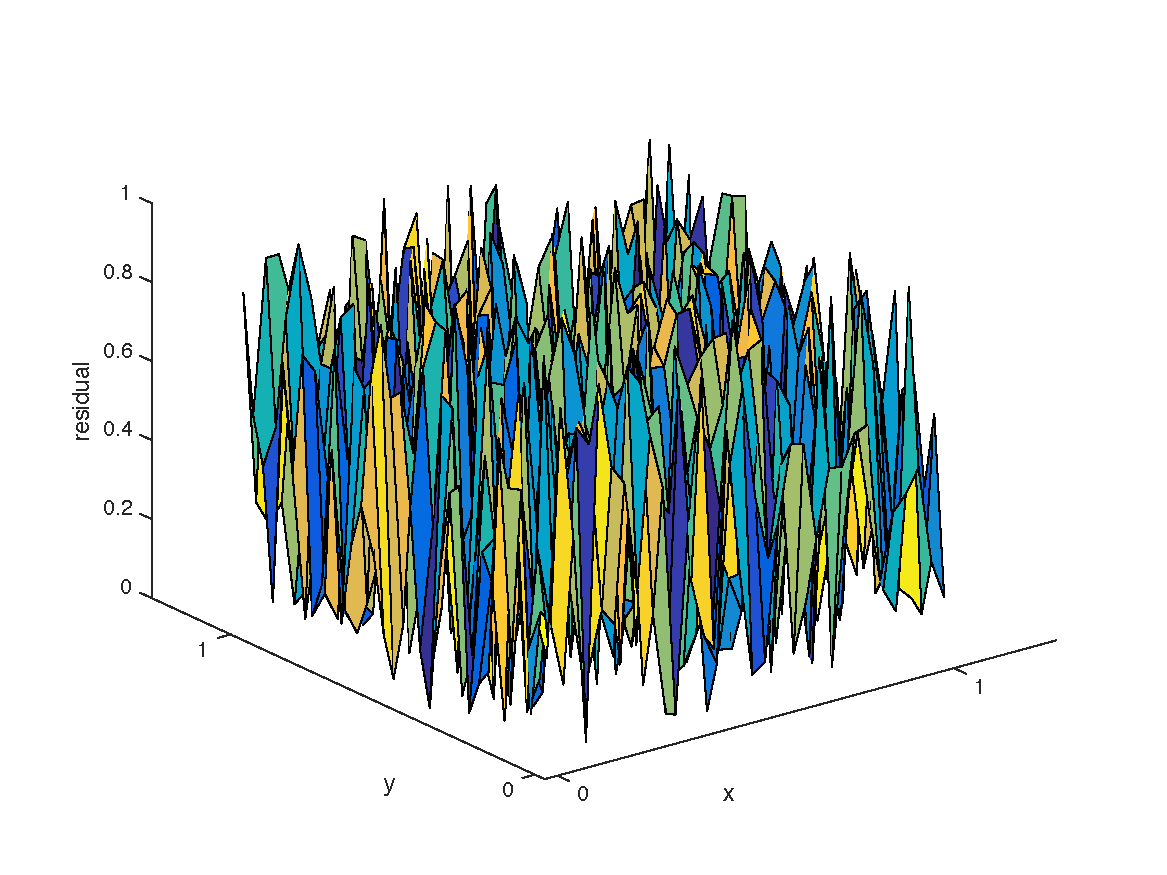
\includegraphics[width=0.5\textwidth]{figures/isotropic_initial}
    \caption{   \eqref{iso-A}    和    \eqref{aniso-A}    的初始错误。  }
    \label{random-exact}
\end{figure}     

   \begin{figure}[!htb]
    \centering
    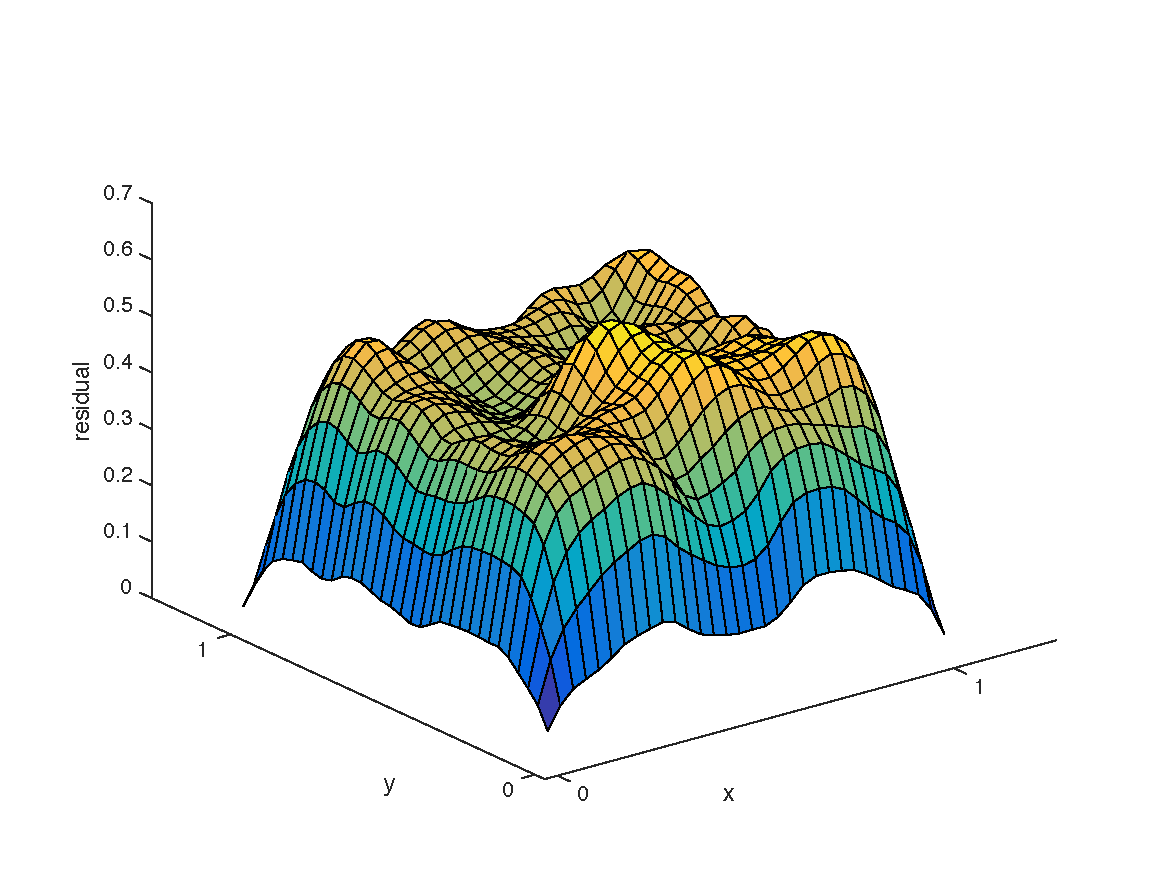
\includegraphics[width=0.3\textwidth]{figures/isotropic_smoothed}
    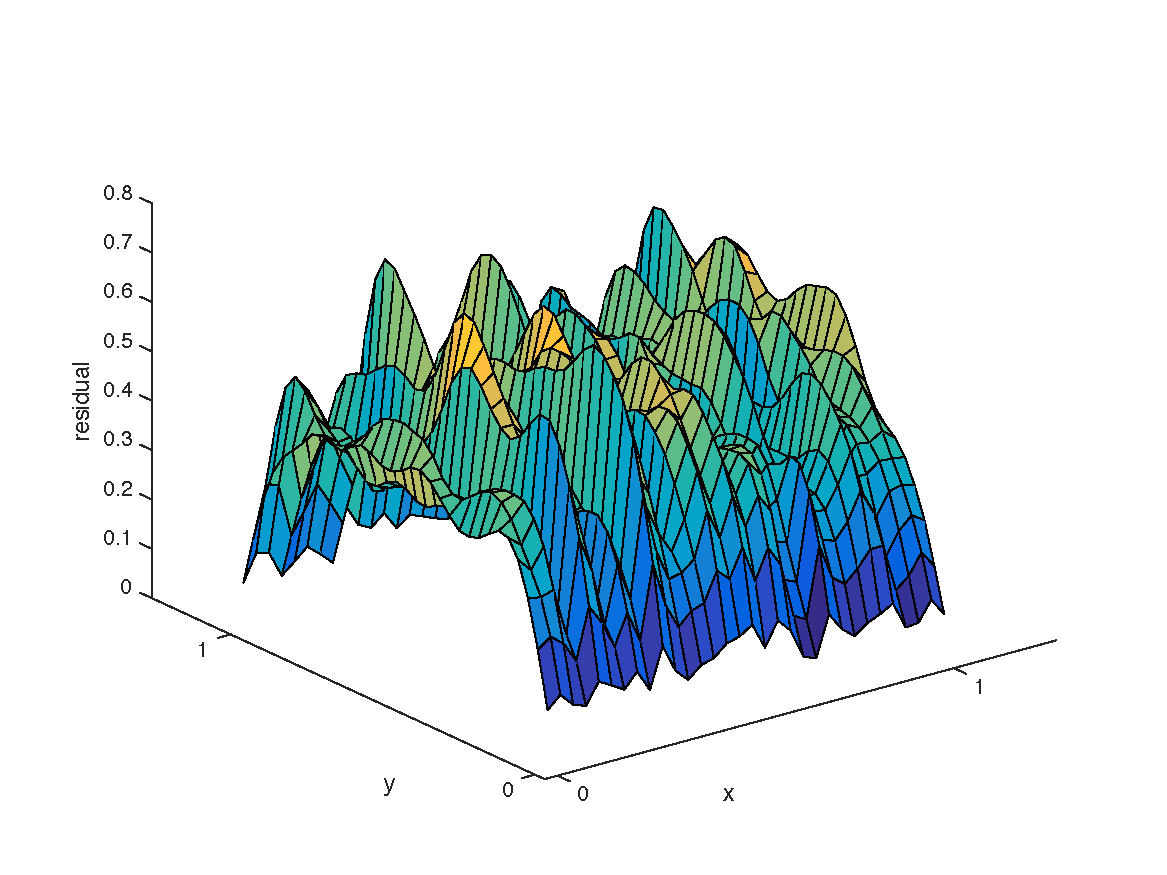
\includegraphics[width=0.3\textwidth]{figures/anisotropic_smoothed}
    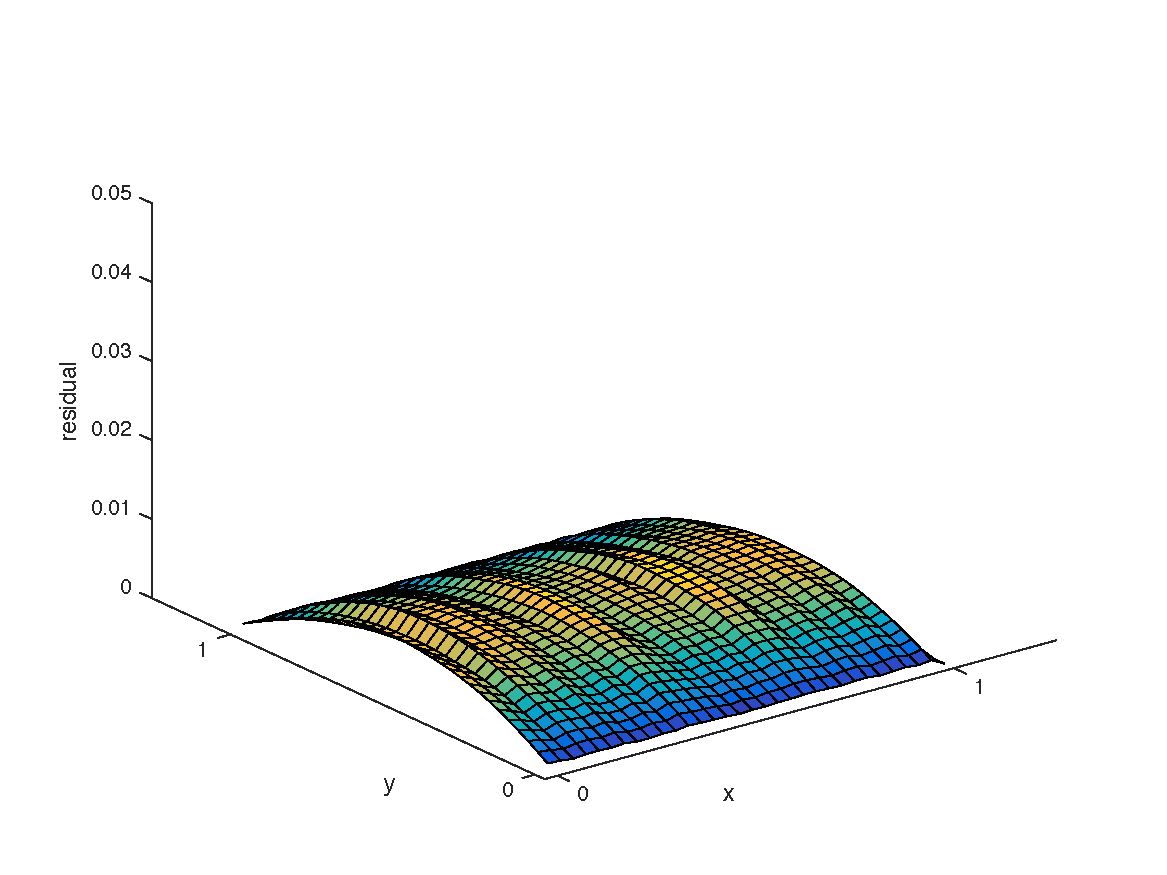
\includegraphics[width=0.3\textwidth]{figures/anisotropic_blk}
    \caption{左图:将    $5$    高斯-赛德尔迭代应用于    \eqref{iso-A}    后的错误。中图:将    $5$    高斯-赛德尔迭代应用于    \eqref{aniso-A}    后的错误。右图:将    $1$    块高斯-赛德尔迭代应用于    \eqref{aniso-A}    后的错误。  }
    \label{f:anisotropic}
\end{figure}     


 
 
 
 
   


 
 
 
 
   

我们注意到,对于    $A$    ,当    $\epsilon\ll 1$    时由    \eqref{aniso-A}    给出,我们有 
   $$
\lambda_{11}<\lambda_{21}< \ldots <\lambda_{N1}<\lambda_{ij}, \quad i\ge
1, j\ge 2.
$$    相应的特征函数,可以看作是“代数低频”,在    $x$    方向上可以高度振荡。  

为了说明代数高/低频与几何高/低频之间的差异,我们考虑    \eqref{aniso-A}    给出的各向异性问题的线性系统。显然,   $A$    可以写成
   \begin{equation*}
    A= \epsilon I\otimes M + M\otimes I \text{ with } M=\operatorname{tridiag}(-1, 2, -1).
\end{equation*}     

我们将向量    $\mu \in R^N$    定义为 
   \begin{equation*}
    \mu=x\otimes y, \text{ with } x=\bm{1}_n, \text{ and } y= (1~0~1~ 0\cdots 1~0~1)^T\in R^n.
\end{equation*}     

然后很容易计算出 
   \begin{equation*}
    Mx= \begin{pmatrix}
        1 \\ 
        0 \\ 
        0 \\ 
        \vdots \\ 
        0 \\ 
        1
    \end{pmatrix}, \text{ and }
    My= \begin{pmatrix}
        2 \\ 
        -2 \\ 
        2 \\ 
        \vdots \\ 
        -2 \\ 
        2 \\  
    \end{pmatrix}.
\end{equation*}    我们有 
   \begin{equation*}
  A\mu = \epsilon (I\otimes M)(x\otimes y)+(M\otimes I)(x\otimes y) = \epsilon (x\otimes My)+(Mx\otimes y),
\end{equation*}    和 
   \begin{eqnarray*}
    \|\mu\|_A^2 &= &\mu^TA\mu= \epsilon (x\otimes y)^T(x\otimes My)+(x\otimes y)^T(Mx\otimes y) \\ 
    &=& \epsilon (x^Tx)\otimes (y^TMy)+(x^TMx)\otimes (y^Ty)=\epsilon n(n+1)+n+1.
\end{eqnarray*}    让    $D$    成为    $A$    的对角线,然后我们有
   \begin{equation*}
    \|\mu\|_D^2 = 2(1+\epsilon)\mu^T\mu= (1+\epsilon)n(n+1).
\end{equation*}    这表明
   \begin{equation*}
    \frac{\|\mu\|_A^2}{\|\mu\|_D^2}= \frac{\epsilon}{1+\epsilon}+\frac{1}{(1+\epsilon)(n+1)},
\end{equation*}    这意味着如果    $\epsilon$    足够小,则    $\mu$    是一个代数低频。  

另一方面,如果我们用    $ \{ \phi_{ij}: 1\le i, j\le n \} $    表示对应于均匀有限元网格的节点基函数,即    $\phi_{ij}$    是一个分段线性函数,使得
   \begin{equation*}
    \phi_{ij}(kh, lh)=\delta_{ik}\delta_{jl}.
\end{equation*}    则我们定义
   \begin{equation*}
    \bm{\Phi}=(\phi_{11}, \phi_{12}, \cdots, \phi_{1n}, \phi_{21}, \cdots, \phi_{nn}).
\end{equation*}    如果我们考虑对应于    $\mu$    的有限元函数,即由
   \begin{equation}\label{fx}
    u= \bm{\Phi}\mu = \sum_{i=1}^{\frac{n+1}{2}}\sum_{j=1}^{n}\phi_{2i-1, j}.
\end{equation}    定义的函数,那么从几何角度来看,该函数在    $x$    方向上高度振荡,这是一个几何高频(见图~    \ref{f:fx}    )  

   \begin{figure}[h]
    \centering
    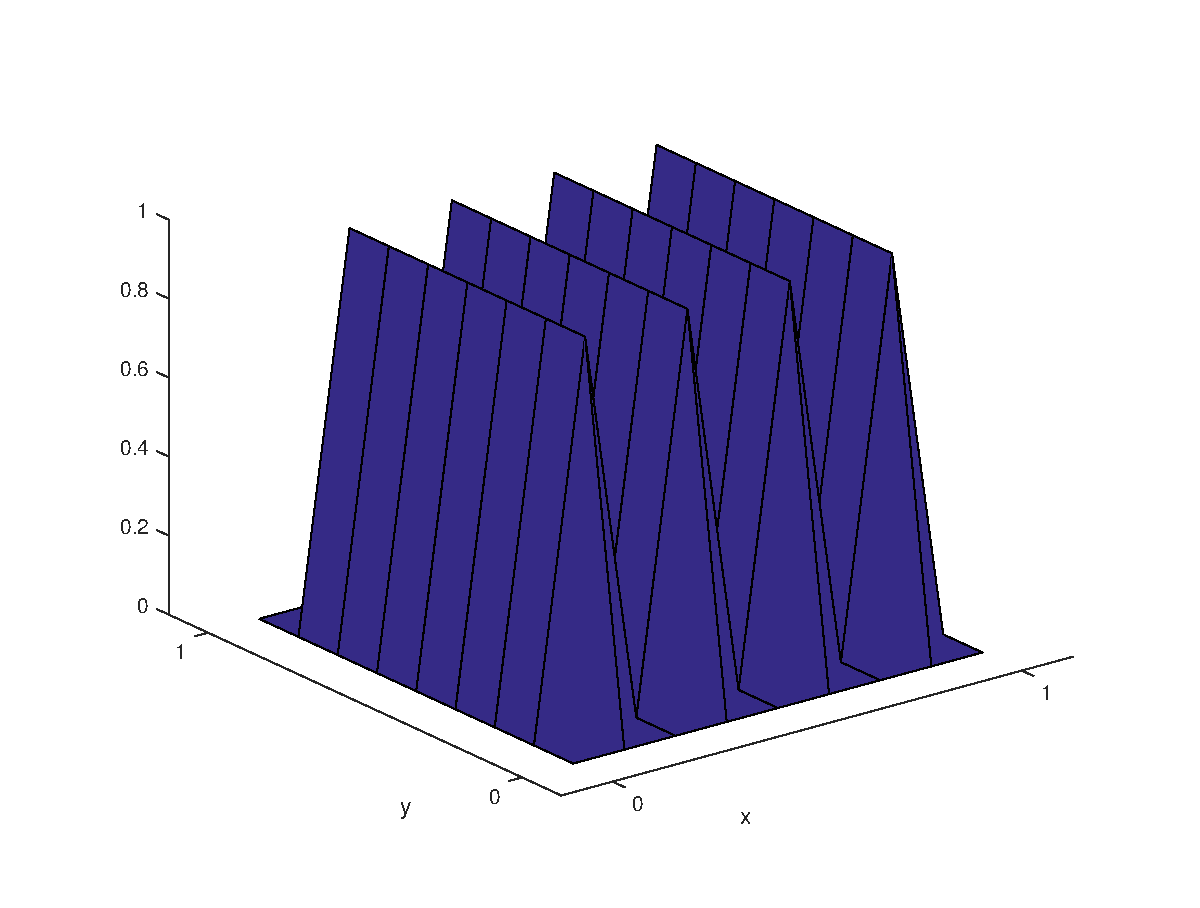
\includegraphics[width=0.6\textwidth]{semicoarse}
    \caption{~    \eqref{fx}    中定义的函数图。此函数在    $x$    方向上振荡剧烈。  }
    \label{f:fx}
\end{figure}     

   \subsection{从代数高频和低频角度看收敛理论  }     

接下来我们提出一种基于代数高频和低频的收敛理论。我们首先证明以下引理。
   \begin{lemma}   \label{l:VhfVc}    如果    $V_c\subset V$    满足以下“稳定分解”:
对于由    $\delta$    代数高频组成的某些    $V_{hf}\subset V$   ,存在    $$
V=V_c+V_{hf}
$$   (参见定义~    \ref{def:high-frequencies}   )。也就是说,对于任何    $v\in V$   ,都存在    $v_c\in V_c$    和
   $v_{hf}\in V_{hf}$   ,使得
   $$
v=v_c+v_{hf}, \quad \|v_{hf}\|_A^2\le c_1\|v\|_A^2.
$$    则相应的 2 级 AMG 满足
   $$
\|E\|_A\le 1-\frac{\delta}{c_1} .
$$     \end{lemma}   
   \begin{proof}因此,
   $$
\inf_{w_c\in V_c}\Tnorm{v-w_c}^2
\le \Tnorm{v_{hf}}^2\le \delta^{-1}\|v_{hf}\|_A^2\le 
\frac{c_1}{\delta}\|v\|_A^2.
$$    结果是,
   $$
K(V_c)\le\frac{c_1}{\delta},
$$    最后,我们得到,
   $$
\|E\|_A=1-\frac{1}{K(V_c)}\le 1-\frac{\delta}{c_1}.
$$     \end{proof}     

   \begin{corollary}   \label{c:AHF}    如果    $V_{hf}$    由    $\delta$    代数高频组成,则对于粗空间    $V_c$   ,由
   \begin{equation}
  \label{quasiVc} V_c= \operatorname{Range}(I-P_{hf}),
\end{equation}    给出,其中    $P_{hf}: V\mapsto V_{hf}$    是 A 正交投影。然后
   $$
\|E\|_A\le 1-\delta .
$$     \end{corollary}     

   \subsection{书目注释  }    关于 AMG 方法的两级收敛的首批结果之一可以在早期论文~    \cite{1stAMG,Ruge.J;Stuben.K.1987a}    中找到。通过代数设置反映 MG 理论的研究有很多:
   \cite{1983MaitreJ_MusyF-aa,1985BankR_DouglasC-aa,Mandel.J.1988a}   ;两级 MG 理论的代数变分方法~    \cite{1985McCormickS-aa,1984McCormickS-aa,1982McCormickS_RugeJ-aa}   。  

对于两个网格收敛,在~    \cite{2008ZikatanovL-aa}    中给出了更清晰的结果,包括两侧边界,在
   \cite{Falgout.R;Vassilevski.P.2004a}    和~    \cite{Falgout.R;Vasilevski.P;Zikatanov.L.2005a}    中也进行了考虑。这些两级结果或多或少是~    \cite{1991BrambleJ_PasciakJ_WangJ_XuJ-ac,1992XuJ-aa,Xu.J;Zikatanov.L.2002a}    中提供的抽象理论的直接结果。最近的一篇文章~    \cite{2014MacLachlanS_OlsonL-aa}    对这些和其他相关结果进行了概述。本节中包含的两种分析方法是最近在
   \cite{UnifiedAMG,EnergyMin}    中开发的。  

定理~    \ref{thm:two-level-convergence}    可以在
   \cite{2008ZikatanovL-aa}    中找到,并且可以看作是子空间校正方法的一般框架中两个子空间的特殊情况下 XZ 恒等式
   \cite{Xu.J;Zikatanov.L.2002a}    的结果。该定理在    \cite{2008ZikatanovL-aa}    中的原始证明基于 XZ 恒等式。这里的证明是新的,更直接。
在一般代数设置中很难建立多级结果,其中大多数结果要么基于不切实际的假设,要么使用几何网格来证明收敛性。我们参考~    \cite{1996VanekP_MandelJ_BrezinaM-aa,2011BrezinaM_VassilevskiP-aa}    来了解这方面的结果。可以使用辅助空间框架推导出有限元方程的严格多级结果,该框架是在~    \cite{1996XuJ-aa}    中为准均匀网格开发的。最近,自适应细化网格的多级收敛结果在~    \cite{2012ChenL_NochettoR_XuJ-aa}    中被证明是最佳的。在~   \cite{2015GrasedyckL_WangL_XuJ-aa}    中显示了使用基于四叉树(二维)和八叉树(三维)粗化的 AMG 在形状规则网格上的多级收敛结果。  

最后,我们指出本节部分内容中使用的符号源自~   \cite{1980BankR_DupontT-aa,bramble1987new,bramble1990parallel}   ,并且便于分析,尤其是在考虑有限元方程时。  

   \section{粗空间构造的通用方法  }       \label{sec:unifiedAMG}    在本节中,我们描述了一个使用空间分解和子空间校正概念构建粗空间的抽象框架。  

我们先介绍一下后面作为分析工具使用的一些技术成果。
   \begin{lemma}   \label{lm:auxiliary}    假设    $\utilde{V}$    和    $V$    为两个向量空间,假设
   $\Pi:\utilde{V}\mapsto V$    为一个全射映射。假设
   $\utilde{B}:\utilde{V'}\mapsto \utilde{V}$    为一个 SPD 算子。则
   $B:=\Pi\utilde{B}\Pi'$    也是 SPD。此外,
   \begin{equation}
  \label{auxi-identity}
    (B^{-1}v,v) =\min_{\Pi\utilde{v}=v}\langle \utilde{B}^{-1}\utilde{v},\utilde{v}\rangle,
\end{equation}    具有由
   \begin{equation}
  \label{minimizer}
  \utilde{v}^*=\utilde{B}\Pi'B^{-1}v.
\end{equation}    给出的唯一最小化器  \end{lemma}   
   \begin{lemma}   \label{l:fictitiousB}    假设    $\Pi$    满足以下两个条件:
   \begin{enumerate}[1.]

    \item   对于所有          $\utilde v\in \utilde V$          , 
   \begin{equation}
          \label{tBA1}
        \|\Pi \utilde v\|_A\le \tilde\mu_1\|\utilde v\|_{\utilde B^{-1}}.
        \end{equation}      \item   对于任何          $v\in V$          ,都存在          $\utilde v \in\utilde V$          ,使得          $\Pi\utilde v=v$          和 
   \begin{equation}
          \label{tBA0}
        \|\utilde v\|_{\utilde B^{-1}}\le \tilde\mu_0\|v\|_A.   
        \end{equation}     \end{enumerate}    然后
   $$
\kappa (BA)\le \left(\frac{\tilde\mu_1}{\tilde\mu_0}\right)^2.
$$     \end{lemma}     

上述引理    \ref{l:fictitiousB}    的直接推论是以下结果。
   \begin{theorem}[Fictitious Space Lemma]   \label{theorem:fictitiousA}    假设    $\Pi$    满足以下两个条件。首先
   $$
\|\Pi \utilde v\|_A\le \mu_1\|\utilde v\|_{\utilde A}, \quad\forall
\utilde v\in \utilde V
$$    其次,对于任何    $v\in V$    ,存在    $\utilde v \in\utilde V$    使得    $\Pi\utilde v=v$    和 
   $$
\|\utilde v\|_{\utilde A}\le \mu_0\|v\|_A. 
$$    然后是    $\kappa(\Pi)\le \mu_1/\mu_0$    并且,在引理    \ref{lm:auxiliary}    的假设下 
   $$
\kappa (BA)\le \left(\frac{\mu_1}{\mu_0}\right)^2\kappa(\utilde B\utilde A). 
$$     \end{theorem}     

我们假设存在一系列空间
   $V_1, V_2, \dots, V_J$    ,它们不一定是
   $V$    的子空间,但它们中的每一个都通过线性算子与原始空间    $V$    相关
   \begin{equation} \Pi_j: V_j\mapsto
      V.  \end{equation}    我们假设    $V$    可以写成子空间之和,并且    \eqref{aux-decomp}    和    \eqref{aux-decomp0}    成立。  

用内积表示
   $$\utilde{W} = V_1\times V_2\times...\times V_J,
$$    ,其中    $\utilde u=(u_1,...,u_J)^T$    和    $\utilde
v=(v_1,...,v_J)^T$    。或者更一般地,对于    $\utilde f=(f_1, \ldots, f_J)^T\in
\utilde V'$    和    $f_i\in V_i'$    ,我们可以定义
   $$
( \utilde f, \utilde v) =\sum_{i=1}^J( f_i, v_i).
$$    我们现在用    $$
\Pi_W\utilde u = \sum_{i=1}^J \Pi_i u_i, \quad\forall \utilde
u=(u_1,...,u_J)^T\in \utilde W. 
$$    定义    $\Pi_W:\utilde W\mapsto V$    正式地,我们可以写成
   $$
\Pi_W=(\Pi_1,\ldots,\Pi_J) \mbox{ and }
\Pi_W'=
\begin{pmatrix}
\Pi_1' \\ 
\vdots \\ 
\Pi_J'
\end{pmatrix}.
$$     

我们假设有一个算子    $A_j: V_j\mapsto V_j'$   ,它是对称的,对每个    $j$    都是半正定的,并定义    $\utilde A_W: \utilde W\mapsto \utilde W'$    如下
   \begin{equation}\label{utildeAW}
      \utilde A_W: = \operatorname{diag}(A_1, A_2, \dots, A_J).
  \end{equation}     

对于每个    $j$    ,我们假设有一个对称正定算子    $D_j: V_j\mapsto V_j'$    ,并定义    $\utilde D:
    \utilde W\mapsto \utilde W'$    如下
   \begin{equation}\label{utildeD}
      \utilde D: = \operatorname{diag}(D_1, D_2, \dots, D_J).
  \end{equation}     

我们将粗空间    $V_j^c$    、    $V_j^c \subset V_j$    与每个空间    $V_j$    关联起来,并考虑相对于
   $(\cdot, \cdot)_{D_j}$    的相应正交投影    $Q_j: V_j\mapsto V_j^c$    。我们通过
   \begin{equation}
        \utilde Q: =\operatorname{diag}(Q_1, Q_2, \dots, Q_J).
    \end{equation}    定义    $\utilde Q: \utilde W\mapsto \utilde W'$     

   \begin{assumption}   \label{a:2level}       \quad    
   \begin{enumerate}

   \item   以下不等式适用于所有          $\utilde w\in \utilde W$          :
对于某个正常数          $C_{p, 2}$          ,    \begin{equation}\label{assm:D_j}
            \|\Pi_W \utilde w\|_D^2\le C_{p,2}\|\utilde w\|_{\utilde D}^2, 
        \end{equation}    成立。   \item   对于每个          $w\in V$          ,存在一个
         $\utilde w\in \utilde W$          ,使得          $w=\Pi_W\utilde w$          和以下不等式成立
   \begin{equation}\label{sum_Aj}
        \|\utilde w\|_{\utilde A_W}^2\le C_{p,1}\|w\|_A^2
\end{equation}    具有一个正常数          $C_{p, 1}$          ,与          $w$          无关。   \item   对于所有          $j$          , 
   \begin{equation}
    \label{NAjVjc}
N(A_j)\subset V_j^c.    
  \end{equation}     \end{enumerate}     \end{assumption}     

   \begin{remark}上述假设意味着 
   $$
w\in N(A) \Rightarrow \utilde w\in N(A_1)\times\ldots \times N(A_J).
$$     \end{remark}     

我们将全局粗空间    $V_c$    定义为 
   \begin{equation}\label{V_c}
    V_c:=\sum_{j=1}^J\Pi_j V_j^c.
\end{equation}     

此外,对于每个粗空间    $V_j^c$    ,我们定义
   \begin{equation}\label{muj}
    \mu^{-1}_j(V_j^c):=\max_{v_j\in V_j}\min_{v_j^c\in V_j^c}\frac{\|v_j-v_j^c\|_{D_j}^2}{\|v_j\|_{A_j}^2},
\end{equation}    和 
   \begin{equation}
  \label{muc}
    \mu_c=\min_{1\le j\le J}\mu_j(V_j^c),
\end{equation}    ,由于假设    \ref{a:2level}    .3 ,它们是有限的(即    \eqref{NAjVjc}    )。  

根据两级收敛理论,如果    $D_j$    提供收敛平滑器,则
   $(1-\mu_j(V_j^c))$    是具有粗空间    $V_j^c$    的    $V_j$    的两级 AMG 方法的收敛速度。下一个定理根据假设~    \ref{a:2level}    和    $\mu_c$    中的常数对两级方法的收敛进行了估计。
   \begin{theorem}   \label{thm:two-level}    如果假设~    \ref{a:2level}    成立,则对于每个    $v\in V$    ,我们有以下误差估计
   \begin{equation}
        \min_{v_c\in V_c}\|v-v_c\|_D^2 \le C_{p,1}C_{p,2}\mu_c^{-1}\|v\|_A^2.
    \end{equation}     \end{theorem}     

   \begin{proof}根据假设~    \ref{a:2level}    ,对于每个    $v\in V$    ,存在    $\utilde v\in \utilde V$    ,使得 
   \begin{equation}
            v=\Pi_W\utilde v
        \end{equation}    和    \eqref{sum_Aj}    得到满足。
根据    $\mu_c$    的定义,我们有
   \begin{equation}
            \|\utilde v-\utilde Q\utilde v\|_{\utilde D}^2\le \mu_c^{-1} \|\utilde v\|_{\utilde A_W}^2.
        \end{equation}    我们让    $v_c=\Pi_W\utilde Q\utilde v$    。然后是    $v_c\in V_c$    ,根据假设~    \ref{a:2level}    ,我们有
   \begin{equation*}
            \|v-v_c\|_D^2 =  \|\Pi_W(\utilde v- \utilde Q\utilde v)\|_D^2 \le  C_{p,2}\|\utilde v-\utilde Q\utilde v\|_{\utilde D}^2 \le  C_{p,2}\mu_c^{-1}\|\utilde v\|_{\utilde A_W}^2\le  C_{p,1}C_{p,2}\mu_c^{-1}\|v\|_A^2.
        \end{equation*}     \end{proof}     

我们定义另一个乘积空间
   \begin{equation}
    \utilde{V}:= V_c\times V_1\times V_2\times \cdots \times V_J,
\end{equation}   ,并将    $\Pi_c: V_c\mapsto V$    设置为从    $V_c$    到    $V$    的自然包含。然后我们通过
   \begin{equation}
    \Pi:=(\Pi_c~\Pi_1~\Pi_2~\cdots~\Pi_J),
\end{equation}    定义    $\Pi: \utilde V\mapsto V$   ,通过
   \begin{equation}
  \utilde A_: = \begin{pmatrix}
      A_c & & &  \\ 
      & A_1 & &  \\ 
      & & \ddots &  \\ 
      & & & A_J  \\ 
      \end{pmatrix},
\end{equation}    定义    $\utilde A: \utilde V\mapsto \utilde V'$   ,其中    $A_c: V_c\mapsto V_c'$    定义为
   \begin{equation}
    A_c: =\Pi_c'APi_c.
\end{equation}   ,而    $\utilde B: \utilde V\mapsto \utilde V'$    定义为
   \begin{equation}
    \utilde B: = \begin{pmatrix}
      A_c^{-1} & & & & \\ 
      & D_1^{-1} & & & \\ 
      & & D_2^{-1} & & \\ 
      & & & \ddots & \\ 
      & & & & D_J^{-1} \\ 
      \end{pmatrix},
\end{equation}     

我们引入加法预条件子    $\widehat B$    
   \begin{equation}\label{additive_B}
    \widehat B: = \Pi \utilde B\Pi' = \Pi_cA_{c}^{-1}\Pi_c' + \sum_{j=1}^J \Pi_j D_j^{-1}\Pi_j',
\end{equation}    并得到以下结果。  

   \begin{lemma}   \label{lem:tBA0}    如果假设~    \ref{a:2level}    成立,则对于任何    $v\in V$    ,都存在    $\utilde v\in \utilde V$    使得    \eqref{tBA0}    成立,即 
   $$\|\utilde v\|_{\utilde B^{-1}}\le \tilde \mu_0\|v\|_A$$    ,其中    $\tilde \mu_0$    是依赖于    $C_{p,1}$    、    $C_{p,2}$    、    $\mu_c$    和    $c^D$    的常数。  \end{lemma}     

   \begin{lemma}   \label{lem:tBA1}    如果假设~    \ref{assm:D_j}    成立,则    \eqref{tBA1}    成立,其中常数    $\tilde \mu_1$    取决于    $C_{p,2}$    和    $c^D$    。  \end{lemma}     

通过直接应用引理~    \ref{l:fictitiousB}    ,我们立即得到
   \begin{theorem}   \label{thm:additive-converge}    如果假设~    \ref{a:2level}    成立,则 
   \begin{equation}
        \kappa (\widehat B A) \le \left(\frac{\tilde \mu_1}{\tilde \mu_0}\right)^2.
    \end{equation}     \end{theorem}     

以下两级收敛结果是收敛定理(定理~    \ref{thm:two-level-convergence}   )与定理~    \ref{thm:two-level}    中的误差估计的应用。  

   \begin{theorem}   \label{thm:two-level-conv}    如果假设~    \ref{a:2level}    成立。则在
   \eqref{V_c}    中定义的粗空间两级 AMG 方法以
   \[
        \|E\|_A^2\le 1-\frac{\mu_c}{C_{p,1}C_{p,2}c^D}.
    \]    的速率收敛  \end{theorem}     

   \subsection{书目注释  }    虚拟空间引理首次在~    \cite{1985MatsokinA_NepomnyashchikhS-aa}    中得到证明。相关工作还包括辅助空间方法~    \cite{1996XuJ-aa}    。引理~    \ref{lm:auxiliary}    的加法版本可在~    \cite{Xu.J;Zikatanov.L.2002a}    中找到,最一般的情况(包括乘法预处理器)可在~    \cite{XuMSC-Notes}    中找到。  

在后面的章节中,我们将展示如何将这里使用的一般理论应用于各种 AMG 算法,例如经典 AMG~    \cite{1stAMG,Ruge.J;Stuben.K.1987a}   、平滑聚合 AMG~    \cite{Mika.S;Vanek.P.1992a,Mika.S;Vanek.P.1992b}   、谱 AMGe~    \cite{Chartier.T;Falgout.R;Henson.V;Jones.J;Manteuffel.T;McCormick.S;Ruge.J;Vassilevski.P.2003b,2011EfendievY_GalvisJ_VassilevskiP-aa}    和其他算法。  

域分解 (DD) 文献中的许多作品也使用了定义粗空间的技术,这些技术在很大程度上与本节概述的 AMG 粗空间构造具有类似的目的。我们参考~   \cite{2005ToselliA_WidlundO-aa,2009WidlundO-aa,1994WidlundO-aa,2008DohrmannC_KlawonnA_WidlundO-aa,2014SpillaneN_DoleanV_HauretP_NatafF_PechsteinC_ScheichlR-aa}    及其参考资料,了解有关在 DD 方法中使用局部特征空间构造粗空间的更多详细信息。  

   \section{图和稀疏矩阵  }       \label{sec:graphs}    在本节中,我们简要介绍一些常用于稀疏矩阵以及 AMG 研究的图论基本概念。  

   \subsection{稀疏矩阵及其邻接图  }       \label{s:ugraph}    无向图(或简称为图)    $\mathcal{G}$    是一对    $(\mathcal{V},\mathcal{E})$    ,其中    $\mathcal{V}$    是一组有限的点(称为顶点),而    $\mathcal{E}$    是一组有限的顶点对(称为边)。我们经常将某些固定的    $n$    写为
   $\mathcal V= \{ 1,\ldots,n \} $    。本文中我们不考虑有向图,因为对应于对称稀疏矩阵的图是无向的。  

边    $e\in \mathcal{E}$    是无序对    $(j,\,k)$    ,其中
   $j,\,k \in \mathcal{V}$    。如果    $(j,k)\in \mathcal{E}$    ,则称顶点    $j$    和    $k$    相邻。从顶点
   $j$    到顶点    $k$    的路径是顶点序列    $(j_0,\,j_1,\,j_2,...,\,j_l)$    ,其中对于所有    $i = 0,\,1, ...,\,l-1$    ,    $j_0=j$    、    $j_l = k$    和    $(j_i,\,j_{i+1}) \in
\mathcal{E}$    。如果有从    $j$    到
   $k$    的路径,则顶点    $j$    连接到顶点    $k$    。如果每对顶点都通过路径连接,则    $\mathcal{G}=(\mathcal{V}, \,\mathcal{E})$    是连接的,否则称为断开的。如果
   $\mathcal{V}_0\subset\mathcal{V}$    和
   $\mathcal{E}_0\subset\mathcal{E}$    ,则图
   $\mathcal{G}_0=(\mathcal{V}_0,\mathcal{E}_0)$    被称为    $\mathcal{G}=(\mathcal{V},\mathcal{E})$    的子图。  

邻域    $N(i)$    是与顶点    $i$    相邻的顶点。顶点的度或价是连接到它的边的数量。这些定义为:
   \begin{equation}\label{ni-di}
    N(i)= \{ j: (i, j)\in \mathcal E \} ,\quad    d_i=| \{ j: (i, j)\in \mathcal E \} |. 
\end{equation}    连接两个顶点    $i$    和    $j$    的路径是边    $(k_0, k_1)$    、   $(k_1, k_2)$    、   \ldots    、   $(k_{m-1}, k_m)$    和
   $\mathcal E$    的序列,使得    $k_0=i$    和    $k_m=j$    。路径的长度是其中的边数。两个顶点
   $i$    和    $j$    之间的距离是连接    $i$    和    $j$    的最短路径的长度,我们用    $\operatorname{dist}(i, j)$    表示它。如果    $i$    、    $j$    不相连,则为    $\operatorname{dist}(i, j)=\infty$    。图的直径是两个顶点之间的最大距离,即
   $\operatorname{diam}(\mathcal G) = \max\limits_{(i, j)\in \mathcal
  E}\operatorname{dist}(i, j)$    。独立集是一组没有两个相邻的顶点。最大独立集是一个独立集,向该集合添加任何其他顶点都会强制该集合包含一条边。  

给定一个对称矩阵    $A \in \mathbb{R}^{n\times n}$    ,    $A$    的邻接图是一个无向图,用
   $\mathcal{G}(A)$    、    $\mathcal{G}= (\mathcal{V}, \,\mathcal{E})$    和
   $\mathcal{V}= \{ 1, \,2, ..., \,n \} $    表示。边    $\mathcal{E}$    定义为
   \[
\mathcal{E} =  \{ (j,\,k)\;\big|\; a_{jk} \ne 0 \} . 
\]    如果矩阵    $A$    的邻接图
   $\mathcal G(A) = (\mathcal V, \mathcal E)$    是连通的,则该矩阵称为不可约的。否则,
   $A$    称为可约的。  

图~    \ref{fig:graph-and-matrix}   (左)显示了对称矩阵的一个示例,图~    \ref{fig:graph-and-matrix}   (右)显示了相应图形的绘制。图形的图形表示通常不可用,并且图形可以用不同的顶点坐标以不同的方式绘制。一般来说,稀疏矩阵不提供底层图形的任何几何信息,而只提供    $\mathcal{G}(A)$    的组合/拓扑属性。  

   \begin{figure}[!htbp]
\begin{center}
\parbox{0.35\textwidth}{        $
A=\begin{pmatrix}
      * & * & * & * & * & *  \\ 
      * & * & * & 0 & 0 & 0  \\ 
      * & * & * & * & * &  0  \\ 
      * & 0 & * & * & * & 0 \\ 
      * & 0 & * & * & * & 0 \\ 
      * & 0 & 0 & 0 & 0 & *   
\end{pmatrix}$        }
\parbox{0.35\textwidth}{\includegraphics*[width=0.3\textwidth]{graph1}}
\end{center}
\caption{稀疏对称矩阵(左)及其相关图(右)。   \label{fig:graph-and-matrix}     }
\end{figure}     

给定 
   $$
S\subset  \{ 1,\ldots,n \} \times \{ 1,\ldots,m \} ,  
$$    我们定义 
   \begin{equation}
  \label{ZS}
\mathbb R_S^{n\times m}=\bigg \{ X=(x_{ij})\in \mathbb R^{n\times m}:  x_{ij}=0 \mbox{ if } (i,j)\notin S\bigg \} 
\end{equation}    我们说    $X$    具有由    $S$    给出的稀疏模式当且仅当    $X\in
\mathbb R_S^{n\times m}$    。  

通常,矩阵的稀疏模式是预先确定的,并且集合    $S$    由给定矩阵确定。对于    $Y\in
\mathbb{R}^{n\times m}$   ,我们表示
   \[
\sparse(Y) = \big \{ (i,j)\;\big|\; y_{ij}\neq 0\big \} .
\]     

我们现在考虑与有限元或有限差分刚度矩阵相关的图形。对于有限元,这是 FE 函数空间
   $V_h$    ,对于有限差分离散化,这是网格函数空间    $V_h$    ,可以将其识别为
   $\mathbb{R}^N$    。  

我们假设我们有一个有限维空间    $V_h^N$   ,我们用它来离散化诺伊曼问题。我们还有用于狄利克雷(或混合边界条件)问题的 FE 空间,并假设以下包含成立    $V_h=V_h^D\subset V_h^N$    。同样地,我们假设自由度的子空间在    $V_h$    上消失:例如,狄利克雷边界上节点的有限元或有限差分解的值消失。  

让    $A^{\mathcal N}$    成为具有 Neumann 边界条件的模型二阶椭圆方程的有限元或有限差分离散化对应的矩阵。显然,我们有以下恒等式,
   \begin{equation}\label{neu}
(A^{\mathcal N}u,v) = \sum_{e\in \mathcal{E}} \omega_e \delta_e u \delta_e v, \quad 
\end{equation}    此处,和是图的所有边    $\mathcal{E}$    上的和
   $\mathcal{G}(A^{\mathcal N}) = (\mathcal{V},\mathcal{E})$    ,如果是    $\mathcal{E}\ni e=(i,j)$    ,则为    $\delta_e v
= v_i - v_j$    ,    $i<j$    。此外,   $\omega_e= -
(A^{\mathcal{N}})_{ij}$    是
   $A^{\mathcal{N}}$    的非对角线项。请注意,由于我们考虑 Neumann 问题,由    $A^{\mathcal{N}}$    定义的双线性形式对于    $u$   (分别为    $v$   )消失,使得对于所有    $i$    ,   $u_i=1$   (分别为    $v_i=1$   )消失。对于 5 点和 9 点模板,我们对所有    $e$    都有    $\omega_e=1$    。  

我们考虑刚度矩阵    $A^{\mathcal N}$    ,它对应于模型问题~    \eqref{Model0}   ,在有界域    $\Omega\subset \mathbb{R}^d$    上具有 Neumann 边界条件,即我们有边界条件:
   \begin{equation}\label{like-laplace}
\alpha\nabla u\cdot\bm{n} = 0, \quad \mbox{on}\quad\partial\Omega,
\end{equation}    其中    $\bm{n}$    是指向    $\partial \Omega$    的单位法向量。很容易推导出对应于狄利克雷或混合边界条件问题的刚度矩阵:我们只需将    $A^{\mathcal N}$    定义的双线性形式限制为子空间:
   \begin{equation}\label{bilinear1}
(Au,v) = \sum_{e\in \mathcal{E}} \omega_e \delta_e u \delta_e v, \quad
u_j=v_j=0\quad x_j\in \Gamma_D.  
\end{equation}    
   \begin{remark}具有自然(诺伊曼)和本质(狄利克雷)边界条件的微分问题之间的类似关系不仅在这里考虑的模型问题中可见,而且在    $H(\curl)$   、   $H(div)$   、线性弹性和其他问题中也可见。  \end{remark}     

   \subsection{   $M$    -有限元刚度矩阵的矩阵亲属  }       \label{sec:m-matrix}    如果对称矩阵    $A \in \mathbb R^{n\times n}$    满足以下三个属性,则称为    $M$    矩阵:
   \begin{align}
\label{eq:sign1} &a_{ii} > 0 \;\;\text{for}\;\; i = 1,...,n, \\ 
\label{eq:sign2} &a_{ij} \le 0 \;\;
                  \text{for}\;\; i \ne j, \;\;i, \;j = 1,...,n, \\ 
\label{eq:sign3} &A \;\;\text{is semi-definite}.
\end{align}     

作为创建空间层次的第一步,具有半正定    $A$    的    $Au = f$    的大多数 AMG 算法使用对    $A$    条目的简单过滤并构造    $M$    矩阵,然后使用该矩阵定义关键的 AMG 组件。
   \begin{definition}[        $M$        -matrix relative]如果矩阵
   $\widetilde A$    为 M 矩阵且满足不等式
   \begin{equation}\label{MMrel-0}
(v,v)_{\widetilde{A}} \lesssim (v,v)_{A}, \quad\mbox{and}\quad
(v,v)_{D}\lesssim (v,v)_{\widetilde{D}}, \quad \mbox{for all} \quad v\in V,
\end{equation}   (其中    $\widetilde D$    和    $D$    分别是    $\widetilde{A}$    和    $A$    的对角线),则我们称矩阵
   $\widetilde A$    为    $A$    的相对    $M$    矩阵。  \end{definition}     

需要说明几点:(1)我们使用术语    $M$    -矩阵来表示半正定矩阵,我们知道这不是精确的定义。但是使用    $M$    -矩阵要方便得多,因此我们决定在这里稍微放宽一下定义,希望这种不准确性能更好地吸引读者;(2)我们指出,受限的    $M$    -矩阵亲属有助于定义粗空间,也有助于估计收敛速度。这在后面的~    \S       \ref{2-level-theory}    中可以清楚地看到,我们在那里介绍了 AMG 的统一二级理论。(3)通常,情况是~    \eqref{MMrel-0}    中的单边不等式实际上是谱等价的。  

根据定义,我们有以下简单但重要的结果。
   \begin{lemma}   \label{lemma-equiv}    让    $A_+$    成为    $A$    的
   $M$    矩阵,并让    $D$    和    $D_+$    分别成为
   $A$    和    $A_+$    的对角矩阵。如果    $V_c\subset V$    是子空间,则如果估计值
   \begin{equation}
  \label{VcA+}
\| u - u_c \|_{D_+}^2\lesssim \|u\|_{A_+}^2  
\end{equation}    成立,则估计值
   \begin{equation}
    \label{VcA}
\|u - u_c\|_D^2\lesssim \|u\|_A^2    
  \end{equation}    对于某个    $u_c\in V_c$    成立。  \end{lemma}    这个结果意味着我们只需要对    $A$    的 M 矩阵进行操作,就可以得到估计值    \eqref{VcA}    。  

在本节中,我们将展示如何构建    $M$    矩阵,该矩阵相对于由具有线性元素的模型问题    \eqref{Model0}    的有限元离散化产生的矩阵。我们首先考虑具有 Neumann 边界条件的各向同性问题    \eqref{like-laplace}    和各向同性    $\alpha=a(x) I$    。在    \eqref{Model0}    中各向异性张量    $\alpha(x)$    的情况下构建 M 矩阵相对项被推迟到    \S       \ref{sec:aniso}    。  

在本节的其余部分,我们对    $\Omega$    的系数和几何形状做出以下假设:
   \begin{itemize}

   \item   域    $\Omega\subset \mathbb{R}^d$    被划分为单纯形
   $\Omega=\cup_{T\in\mathcal{T}_h} T$    。   \item   系数    $a(x)$    是一个标量值函数,其不连续性与分区    $\mathcal{T}_h$    对齐。   \item   我们考虑诺伊曼问题,因此双线性形式~    \eqref{Vari}    是
   \begin{equation}\label{auv}
\int_{\Omega}a(x) \nabla v \cdot \nabla u  = 
\sum_{(i,j)\in \mathcal{E}} (-a_{ij})\delta_eu\delta_e v 
=\sum_{e\in \mathcal{E}} \omega_e\delta_eu\delta_e v.
\end{equation}      \item   众所周知,刚度矩阵    $A$    的非对角线项由    \begin{eqnarray*}
&& \omega_e  =  -(\phi_j,\phi_i)_A = \sum_{T\supset e}\omega_{e,T} \\  
&& \omega_{e,T} = \frac{1}{d(d-1)}\overline{a}_T |\kappa_{e,T}|\cot\alpha_{e,T}, \quad
\overline a_T= \frac{1}{|T|}\int_{T} a(x) \; dx.
\end{eqnarray*}    给出。其中,   $e=(i,j)$    是一条固定边,其端点为    $x_i$    和    $x_j$    ;
   $T\supset e$    是包含    $e$    的所有元素的集合;
   $|\kappa_{e,T}|$    是    $T$    中与    $e$    相反的    $(d-2)$    维单纯形的体积;   $\alpha_{e,T}$    是    $T$    中不包含    $e$    的两个面之间的二面角。   \item   令    $\mathcal{E}$    表示三角剖分定义的图中的边集,令    $\mathcal{E}^{-}$    表示边集,其中
   $a_{ij}\ge 0$    、    $i\neq j$    。与    $\mathcal{E}^-$    互补的集合是
   $\mathcal{E}^+=\mathcal{E}\setminus\mathcal{E}^-$    。然后,通过
   $\omega_e = -a_{ij}$    、    $\delta_e u=(u_i-u_j)$    、    $e=(i,j)$    ,我们得到
   \begin{equation}\label{auv-do}
\int_{\Omega}a(x) \nabla v \cdot \nabla u  = 
\sum_{e\in \mathcal{E}^+} \omega_e\delta_eu\delta_ev-\sum_{e\in \mathcal{E}^-} |\omega_e|\delta_eu\delta_ev. 
\end{equation}      \item   我们还假设分区使得常数函数是双线性形式~    \eqref{auv}    的零空间中的唯一函数。当然,当    $\Omega$    连通时就是这种情况(这是正确的,因为    $\Omega$    是一个域)。  \end{itemize}     

   $A$    的非零非对角线项可以有正号也可以有负号,通常为    $\mathcal{E}^-\neq \emptyset$    。下一个定理表明,通过双线性形式~    \eqref{auv}    定义的刚度矩阵    $A$    在光谱上等价于定义为
   \begin{equation}\label{diag-compensate}
(A_+ u,v) = \sum_{e\in \mathcal{E}^+} \omega_e (u_i-u_j)(v_i-v_j). 
\end{equation}    的矩阵    $A_+$    。因此,我们可以忽略    $A$    中的任何正非对角线项,或者等效地,我们可以丢弃    $e\in \mathcal{E}^-$    的所有    $\omega_e$    。实际上,   $A_+$    是通过将所有正的非对角线元素添加到对角线并将相应的非对角线元素设置为零而从    $A$    获得的。这是我们稍后需要的更强的结果,因为它给出了与    $M$    矩阵相对    $A_+$    的光谱等价性。
   \begin{theorem}   \label{m-matrix-plus}    如果    $A$    是对应于    \eqref{Model0}    的线性有限元离散化的刚度矩阵,其边界条件由~    \eqref{like-laplace}    给出。则    $A_+$    是相对于    $A$    的    $M$    矩阵,其谱等效于    $A$    。等效常数仅取决于网格的形状规律性。此外,对应于    $A_+$    的图是连通的。  \end{theorem}     

我们稍后将使用一个简单的推论来证明收敛速度的估计,如下所示。
   \begin{corollary}   \label{corollary-diag}    假设    $A$    是方程~    \eqref{auv}    的分段线性离散化的刚度矩阵,   $A_+$    是定理~    \ref{m-matrix-plus}    中定义的相关    $M$    矩阵。则    $A$    的对角线    $D$    和    $A_+$    的对角线    $D_+$    在谱上是等价的。  \end{corollary}   
   \begin{proof}对于    $A$    和    $A_+$    的对角线元素,我们有
   \[
[D]_j = (\phi_j,\phi_j)_A \eqqsim (\phi_j,\phi_j)_{A_+} =[D_+]_j.
\]    上面写的等价关系直接来自引理~    \ref{m-matrix-plus}    。  \end{proof}     

推论   \ref{corollary-diag}   与引理~   \ref{lemma-equiv}   为利用M矩阵相对设计有限元矩阵的AMG提供了理论基础。  

   \subsection{书目注释  }    我们介绍了图论中的一些标准概念。对于对更详细描述感兴趣的读者,我们参考经典教科书~    \cite{2010DiestelR-aa,1985GibbonsA-aa}    作为图论的一般介绍;并参考    \cite{2003SaadY-aa}    、
   \cite{2000VargaR-aa}    来考虑链接图、稀疏矩阵和迭代方法。  

我们关于    $M$    -矩阵相关项的结果与关于    $Z$    -矩阵和
   $L$    -矩阵~    \cite{kraus2006algebraic,kraus2008algebraic}    预处理的一些工作有关。它们隐式地用于大多数 AMG 文献~    \cite{Ruge.J;Stuben.K.1987a}    中,其中经典的连接强度定义给出    $M$    -矩阵。我们指出,
   $M$    -矩阵性质和    $M$    -矩阵相关项的存在通常不足以实现 AMG 的两级一致收敛。一个典型的例子是重新缩放的矩阵,常数不再位于离散算子的核中。在这种情况下,标准 AMG 应用程序可能会失败,并且需要通过不同的方式恢复近核,例如在~    \S       \ref{s:adaptiveAMG}    和其中给出的参考文献中考虑的自适应 AMG 过程。  

   \section{连接强度  }       \label{sc:strength}    
   \newcommand{\cs}     { s\_c   }  AMG 中的一项核心任务是获得适当的粗化空间或延长。此过程称为粗化过程。在几何网格中,或者更一般地说,在刚度矩阵的邻接图中,我们需要识别要从图中删除的顶点。我们需要粗化图仍然为代数低频提供良好的近似值。  

   \subsection{基本思想和强度函数  }    如果顶点子集上的代数平滑向量(例如    $v$    )变化非常缓慢,则我们只需保留一个自由度来表示此子集中的    $v$    。换句话说,我们可以将这个子集聚合在一起,也可以保留其中一个顶点并删除此子集中的其余顶点。我们说这个子集中的顶点彼此紧密相连。连接强度是一个为识别强连接的顶点对而引入的概念。粗略地说,如果
   $v_i\approx v_j$    ,我们说    $i$    和    $j$    是强连接的。  

我们设想通过两个不同的步骤来粗化图形:第一步是删除一些边,第二步是删除一些顶点。第二步是目标。让我们检查一下第二步是如何进行的:我们要么 (1) 将一些相邻顶点聚合在一起,要么 (2) 在过滤后的图形中选择一个 MIS,表示为    $\mathcal C$    ,然后删除所有剩余的顶点。使用上面的论点,(1) 每个聚合应该只由强连接组成,或者 (2) 所有被删除的顶点中的每一个都应该与    $\mathcal C$    中的某个点强连接。为了保证这两种情况中的任何一种,我们必须在第一步中删除所有弱连接的边。  

让我们进一步使用一些启发式论据来激发如何定义连接强度。 让    $v$    成为代数平滑的    \eqref{smoothing-1-norm}    ,即
   $$
\|v\|_A^2\le\epsilon \|v\|_{\bar R^{-1}}^2.
$$    让    $u=v/\|v\|_{\bar R^{-1}}$    ,然后我们有
   \begin{equation}
  \label{slow}
(Au,u) \le\epsilon\Rightarrow \sum_{e=(i,j)\in \mathcal{E}}
(-a_{ij})(u_i-u_j)^2\le \epsilon.
\end{equation}    感谢引理    \ref{lem:eAeD}    ,我们可以假设    $A$    是一个 M 矩阵,即    $-a_{ij}=|a_{ij}|$    。从    \eqref{slow}    可知,我们有以下观察结果:
   \begin{enumerate}

   \item   较大的    $|a_{ij}|$    意味着较小的    $(u_i-u_j)^2$   ;   \item   代数平滑误差在    $|a_{ij}|$    较大的方向上变化得更慢;  \end{enumerate}    观察结果可得出以下连接强度定义:给定阈值    $\theta>0$    ,我们称邻接图的顶点    $j$    为    $\theta$    - 如果
   \begin{equation}\label{classical-strength}
-a_{ij}\geq\theta\max_{k\neq i}-a_{ik}
\end{equation}    则与顶点
   $i$    强连接。我们注意到,根据上述定义,我们可能将    $j$    与    $i$    强连接,而将    $i$    与    $j$    弱连接。因此,具有强连接的矩阵对应的邻接图可能不对称。  

但我们的理论框架是根据对称算子    $\bar R$    给出的,无论原始平滑器    $R$    是否对称。这是因为我们使用能量范数(即    $A$    范数)来测量收敛速度,而最终的收敛速度是根据    $\bar R$    给出的。这是我们拥有的最佳收敛理论,我们将使用该理论来研究 AMG 算法。因此,我们将仅考虑对称的强度函数。与 SSPD 矩阵相关的强度函数是这样的  

   \begin{equation}
  \label{sc-vertices}
\cs : \mathcal V\times\mathcal V\mapsto \mathbb R_{+},
\end{equation}    是对称的,即    $\cs(i,j)=\cs(j,i)$    。  

给定阈值    $\theta>0$    ,如果    $$
\cs(i,j)
\ge \theta.
$$    满足以下条件,我们称    $i$    和    $j$    是    $\theta$    -强连通的:
   $$
\cs(i,j)
\ge \theta.
$$    然后我们定义强度矩阵:
   \begin{equation}\label{defS}
S=\sum_{\cs(i,j)\ge\theta} e_ie_j^T.
\end{equation}     

请注意,   $S$    是一个布尔矩阵,其条目等于 0 或 1,具体取决于连接强度。  

考虑非重叠分解
   \begin{equation}
  \label{Vagg}
    \mathcal V=\bigcup_{i=1}^m\mathcal A_i=\bigcup_{\tilde{\mathcal A}\in \mathcal V_{\mathcal A}}\tilde{\mathcal A}, \quad 
\mathcal V_{\mathcal A} =(\mathcal A_1, \ldots, \mathcal A_m).
\end{equation}    我们扩展强度函数的定义
   \begin{equation}
  \label{sc-patches}
    \cs: \mathcal V_{\mathcal A} \times\mathcal V_{\mathcal A} \mapsto \mathbb R_{+}.
\end{equation}    并假设    $\cs$    是对称的。  

给定一个阈值    $\theta>0$    ,如果 
   $$
\cs(\mathcal A_i,\mathcal A_j)
\ge \theta.
$$    ,我们说    $\mathcal A_i$    和
   $\mathcal A_j$    是    $\theta$    -强连接的。这种强度函数的一个示例在~    \eqref{sc-agg}    中给出。  

在 AMG 文献中,提出了许多用于识别强连接的启发式方法,特别是在考虑各向异性方程的离散化时。一般来说,连接强度是一个难以从理论上解决的概念,也很难将其与算法的收敛速度联系起来。我们参考了~    \S       \ref{s:coarsening-biblio}    中提到的经典论文和专著,以进一步讨论相关问题。AMG 开发的当前趋势旨在重新评估连接强度的经典定义的作用。  

最后,我们想说的是,连接强度用于定义    $P$    的稀疏性,它至关重要,例如,在证明具有跳跃系数的椭圆方程离散化的两级方法的收敛性时。选择    $P$    的“正确”稀疏性至关重要,因为更密集的    $P$    会导致从更粗糙的空间进行更好的近似;而更稀疏的    $P$    会导致更便宜的算法。  

在本节的其余部分,我们讨论了连接强度的不同定义:
   \begin{enumerate}

   \item   经典 AMG;   \item   精益 AMG;   \item   基于局部优化。  \end{enumerate}     

   \subsection{经典AMG  }       \label{s:strength}    基于上述动机,我们定义强度函数如下:
   \begin{eqnarray}
\cs(i,j)& =&\frac{-a_{ij}}{\min\bigg(\max_{k\ne i}(-a_{ik}),
  \max_{k\ne j}(-a_{jk})\bigg)} \nonumber
 \\ 
&=&\frac{a_{ij}}{\max\bigg(\min_{k\neq i}a_{ik}, \min_{k\neq j}a_{jk}\bigg)}. 
\label{sc-cAMG}
\end{eqnarray}       \eqref{sc-cAMG}    的定义是经典 AMG 文献中使用的强度函数的对称版本(参见    \eqref{classical-strength}    )。  

以下定义在经典 AMG 算法中也常用
   \begin{equation}\label{def:strong-connection-2}
\cs(i,j)=\frac{|a_{ij}|}{\min\bigg(\frac{1}{|N(i)|}\sum_{k\neq i}|a_{ik}|, \frac{1}{|N(j)|}\sum_{k\neq i}
|a_{jk}|\bigg)}.
\end{equation}    同样,这是 AMG 文献中使用的强度函数的对称版本。  

最后,我们还可以得到以下两个基于柯西-施瓦茨的 SSPD 矩阵定义:
   \begin{equation}\label{strong-connection-1}
s_1(i,j)=\frac{|a_{ij}|}{\sqrt{a_{ii}a_{jj}}} 
\end{equation}    和 
   \begin{equation}\label{strong-connection-2}
s_2(i,j)=\frac{-2a_{ij}}{a_{ii}+a_{jj}} 
\end{equation}     

请注意,定义    \eqref{sc-cAMG}    (主要与经典 AMG 相关)忽略了刚度矩阵    $A=(a_{ij})$    的所有非负项。  


   


   

   \subsection{局部优化强度函数  }    假设索引    $ \{ i, j \} \subset  \{ 1, \dots, n \} $    的每一对都与一个空间    $V_{ij}$    相关联,该空间不一定是    $V$    的子空间。现在假设我们有两个运算符:   $A_{ij}: V_{ij}\mapsto V_{ij}'$    是对称正定的,半正定的,   $D_{ij}: V_{ij}\mapsto V_{ij}'$    是 SPD。  

给定一个数字    $k_{ij}< \dim V_{ij}$    ,我们定义一个粗空间    $V_{ij}^c\subset V_{ij}$    如下
   \begin{equation*}
    V_{ij}^c:=\operatorname{span} \{ \zeta_{ij}^{(k)}, k=1: k_{ij} \} ,
\end{equation*}    其中    $\zeta_{ij}^{(k)}$    是特征向量,对应于    $D_{ij}^{-1}A_{ij}$    的第    $k$    个最小特征值。  

我们将    $Q_{ij}: V_{ij}\mapsto V_{ij}^c$    表示为相对于    $(\cdot, \cdot)_{D_{ij}}$    的正交投影。受    \eqref{muj}    启发,我们将强度函数    $\cs$    定义如下
   \begin{equation}\label{local-opt-sc}
    \cs(i, j):=\left(\sup_{v\in V_{ij}}\frac{\|(I-Q_{ij})v\|_{D_{ij}}^2}{\|v\|_{A_{ij}}^2}\right)^{-1}.
\end{equation}     

AGMG 引入了上述定义的一个特例。假设现在我们有一组聚合    $ \{ \mathcal A_1, \dots, \mathcal A_J \} $    。我们固定一对    $ \{ i, j \} \subset  \{ 1, \dots, J \} $    ,并定义 
   $$G=\mathcal A_i\bigcup \mathcal A_j.$$    然后我们通过    $V_{ij}$    定义    $V$    对    $G$    的限制,如下所示 
   \begin{equation}
    V_{ij}:= \{ \left.v\right|_{G}: v\in V \} ,
\end{equation}    其中 
   \begin{equation*}
    \left. v\right|_{G}(x)= \begin{cases}
        v(x), & \text{ if } x\in G, \\ 
        0, & \text{ if } x\notin G.
    \end{cases}
\end{equation*}    我们分别用    $A_{ij}$    和    $D_{ij}$    表示    $A$    和    $D$    对    $G$    的限制。然后我们选择    $k_{ij}=1$    并定义局部粗空间    $V_{ij}^c$    
   \begin{equation*}
    V_{ij}^C= \Span \{ \zeta_G \} , \quad \zeta_G=\zeta_{ij}^{(1)}.
\end{equation*}    和    $Q_{ij}: V_{ij}\mapsto V_{ij}^C$    相对于    $(\cdot, \cdot)_{D_{ij}}$    的正交投影,即
   \begin{equation*}
    Q_{ij}v = \frac{(v, \zeta_G)_{D_{ij}}}{\|\zeta_G\|_{D_{ij}}^2}\zeta_G.
\end{equation*}    基于聚合的强度函数定义如下:
   \begin{equation}\label{sc-agg}
    \cs(i, j):=\left(\sup_{v\in V_{ij}}\frac{\|(I-Q_{ij})v\|_{D_{ij}}^2}{\|v\|_{A_{ij}}^2}\right)^{-1}.
\end{equation}     

另一个例子是选择    $V_{ij}=\mathbb{R}^2$    和 
   \begin{equation*}
    A_{ij}=  \begin{pmatrix}
        a_{ii} & a_{ij} \\ 
        a_{ij} & a_{jj}
    \end{pmatrix}, \quad
        D_{ij}= \begin{pmatrix}
        a_{ii} & 0 \\ 
        0 & a_{jj}
    \end{pmatrix}.
\end{equation*}    我们选择    $k_{ij}=1$    并定义粗空间    $V_{ij}^c\subset V_{ij}$    如下
   \begin{equation*}
    V_{ij}^c=\operatorname{span}\left \{  \begin{pmatrix}
        1 \\ 
        1
    \end{pmatrix}  \right \} .
\end{equation*}    通过直接计算,我们得到    \eqref{local-opt-sc}    中定义的强度函数为 
   \begin{equation}\label{scij}
\cs(i, j)= \frac{1-s_1^2}{1-s_2}, \quad s_1=\frac{|a_{ij}|}{\sqrt{a_{ii}a_{jj}}}, \quad s_2=-\frac{2a_{ij}}{a_{ii}+a_{jj}}.
\end{equation}    我们注意到    $s_1\ge s_2$    因此
   \begin{equation}\label{e:s1s2}
        \cs(i, j) \le 1+s_2 \le 1+s_1.
    \end{equation}     

我们想指出的是,
   \eqref{scij}    给出的强度函数是利用
   \S       \ref{sec:unifiedAMG}    中的理论得到的,而其他强度函数如
   \eqref{sc-cAMG}    则是通过启发式考虑得到的。  

   \subsection{精益AMG  }    Lean AMG 不使用矩阵项的绝对值作为判断两点是否强耦合的标准,而是使用亲和力来衡量连接强度,这基于以下启发式观察:  

给定一个向量    $v$    ,如果    $(i, j)$    是一对强连通的顶点,则在对    $v$    进行几次松弛之后,即
   \begin{equation*}
    v\leftarrow (I-RA)^{\nu}v,
\end{equation*}    ,    $v_i$    和    $v_j$    的值应该接近。  

在 Lean AMG 中,我们生成    $K$    测试向量 (TV)。每个 TV 都是将    $\nu$    GS 松弛扫描应用于    $Ax=0$    的结果,从随机生成的向量    $x^{(1)}, \dots, x^{(K)}\in \mathbb R^n$    开始。我们表示 
   \begin{equation}
    X_{n\times K}:= \begin{pmatrix}
        X_1^T \\ 
        \vdots \\ 
        X_n^T
    \end{pmatrix}= (I-RA)^{\nu}
    \left(x^{(1)}~\dots~x^{(K)}\right).
\end{equation}    这里    $X_i^T$    是    $X_{n\times K}$    的第    $i$    行。然后 Lean AMG 的强度函数定义如下
   \begin{equation}\label{sc-Lean}
    \cs(i,j):=\frac{|(X_i, X_j)|^2}{(X_i, X_i)(X_j, X_j)}
\end{equation}     

   \subsection{书目注释  }    确定连接强度的经典算法可以在~    \cite{1stAMG,Stuben.K.1983a,Brandt.A;McCormick.S;Ruge.J.1985a,Ruge.J;Stuben.K.1987a,Briggs.W;Henson.V;McCormick.S.2000a}    中找到。~    \cite{ruge5110final,mccormick1989algebraic,Brandt.A;McCormick.S;Ruge.J.1985a,ruge1983algebraic}    中给出的原始连接强度测量是不对称的,但出于理论考虑,这仅取决于对称平滑器,使用稍微更严格但对称的连接强度版本就足够了。  

这些用于定义强连接的经典算法的一些扩展基于不同的连接性和距离度量,例如重要性度量和代数距离。详细信息请参阅    \cite{Ruge.J;Stuben.K.1987a}    和    \cite[Appendix~A]{Trottenberg.U;Oosterlee.C;Schuller.A.2001a}   。  

连接强度度量在过去几乎没有理论支持。本节中开发的结果(例如局部庞加莱\'{e} 不等式,尤其是强度函数~   \eqref{e:s1s2}   )表明,此类启发式方法是合理的,并且其选择可以由理论结果来推动。  

对于聚合 AMG,通常使用如~   \cite{1996VanekP_MandelJ_BrezinaM-aa}    中定义的对称连接强度函数。一些最近的聚合算法也根据尖锐的理论结果定义连接强度,并使用局部两级收敛速度~   \eqref{local-opt-sc}    作为度量~   \cite{Notay.Y.2010b,Napov.A;Notay.Y.2012a}   。  

对于基于匹配的聚合(大小为    $2$    的聚合),   \cite{Karypis.G;Kumar.V.1998a}    中的“重边”匹配算法对应于根据邻接图中的边权重选择聚合的连接强度函数。最近的一些作品    \cite{Livne.O;Brandt.A.2012a}    使用基于由一组平滑测试向量形成的 Gramm 矩阵中的条目大小的连接强度函数。  

   \section{粗化策略  }       \label{sc:connection}    一旦确定了平滑器,AMG 方法的核心任务就是确定一系列粗空间,用函数术语来说,或者用代数术语来说,就是确定一系列延长矩阵。这个过程称为“粗化”过程。在本节中,我们将讨论如何实现这一粗化过程。  

粗略地说,给定向量空间    $V$    上的方程    \eqref{Au=f}    (即    $Au=f$    ),目标是找到一个子空间    $V_c\subset V$    ,使得以下“粗化”问题的解    $u_c\in V_c$   :
   \begin{equation}
  \label{Ac}
A_cu_c=f_c, \quad A_c=\imath_c'A\imath_c, f_c=\imath_c'f  
\end{equation}    将提供对原始解    $u\in V$    的良好近似。更具体地说,   \eqref{Ac}    的    $u_c$    的解将提供对误差的那些“代数平滑”分量的良好近似,而给定的平滑器不能很好地收敛。  

   \subsection{动机  }    从某种意义上说,“粗化”几乎在数值分析中无处不在。例如,有限元方程    \eqref{vph}    可以看作是原始方程    \eqref{Vari}    的粗化方程。在这种情况下,有限元空间    $V_h$    是    $V=H_0^1(\Omega)$    的粗化子空间。  

因此,研究有限元空间的一般构造方法对我们很有帮助。虽然构造有限元空间的方法有很多种,但从数学上讲,最方便的方法是使用“自由度”,它指的是对偶空间的基础。更具体地说,在有限元离散化中,有限元空间    $V_h$    是通过首先指定对偶空间    $V_h'$   (所谓的自由度空间)获得的。对于线性有限元,   $V_h'= \{ \psi_i:i=1:n_h \} $    是这样的
   $$
\psi_i(v)=v(x_i^h).
$$    有了这样的自由度(节点评估),我们就可以找到对偶基    $ \{ \phi_i: i=1:n_h \} $   ,它们是分段线性函数,使得
   $$
\psi_i(\phi_j)=\delta_{ij}, \quad 1\le i, j\le n. 
$$    有限元空间    $V_h$    然后定义为 
   $$
V_h=\Span  \{ \phi_i: i=1:n_h \} .
$$    事实上,从数学上讲,所有现有的有限元空间
   $V_h$    都可以通过首先构造    $V_h$    来获得。这是有限元方法经典文献中采用的方法,参见    \cite{2002CiarletP-aa}    。  

因此,与有限元方法类似,我们将重点介绍通过首先确定其对偶基    $V_c'$    来构建粗空间    $V_c\subset V$    的技术。这种方法相当抽象,但事实证明它更内在、更通用,而且事实上在 AMG 文献中更常用(隐式)。  

值得注意的是,我们在几何多重网格方法的设计中很少使用“粗化”这个词。相反,我们使用“细化”过程来定义嵌套空间序列。例如,图    \ref{fig-refinement}    显示了用于离散化具有线性有限元的泊松方程的均匀细化三角网格。  

在 AMG 中,我们没有几何细化给出的空间层次结构。相反,我们对细化过程进行逆向工程,即  {    \it    粗化。   }   

   \begin{figure}[!htb]
\centering
\includegraphics*[width=0.3\textwidth]{ref0}
~~\includegraphics*[width=0.3\textwidth]{ref1}
~~\includegraphics*[width=0.3\textwidth]{ref2}
\caption{粗网格元素的常规细化。   $\bullet$    - 最粗级顶点,   $\circ$    - 第一级细化,   $\Box$    - 第二级细化。   \label{fig-refinement}     }
\end{figure}     

可以想象,至少在某些特殊情况下,我们也可以使用这种逆向工程过程,从最精细的几何网格开始恢复几何多重网格法。例如,如果如图    \ref{fig-refinement}    所示的三角剖分中的所有三角形都是锐角类型,则与网格相对应的图也是刚度矩阵的邻接图。很明显,粗网格顶点,即集合    $\mathcal{C}$   (从细化中得知),是与细化网格相对应的图中顶点的最大独立集 (MIS)。在最简单的情况下,与粗网格相关的自由度(   $V_c$    的对偶基础)与 MIS 精确相对应。稍后在经典 AMG 框架中构建算法以通过    \S       \ref{s:MIS}    中的 MIS 算法选择粗网格顶点时,将探讨这种观察结果。有关几何 AMG 和 GMG 粗化之间关系的更多示例,请参阅~    \S       \ref{s:amg-from-gmg}    。  

上述 GMG 逆向工程过程提示了 AMG 中粗化过程的实现方式,但我们需要在更广泛的框架中研究该过程,更重要的是,我们将使用自由度(即对偶基的基)来获得粗化空间。在上述 GMG 示例中,几何网格中的每个网格点都精确对应一个自由度。但在应用中并非总是如此。  

   \subsection{基本方法  }    通过模仿上面描述的有限元空间的构造,给定方程    $Au=f$    的线性代数系统,我们采用由以下步骤组成的粗化策略:  

   \begin{enumerate}

   \item   我们考虑系数矩阵    $A$    的邻接图    $\mathcal G(A)$    。基于    \S       \ref{sc:strength}    中描述的某种强度函数    $s_c$    ,我们删除    $\mathcal G(A)$    中的弱连通边,即删除    $A$    中的某些条目,以形成滤波矩阵    $\tilde A$    。   \item   我们执行以下两项之一:
   \begin{enumerate}      \item   经典 AMG:找到    $\mathcal G(\tilde A)$    的一个 MIS 来形成粗顶点集    $\mathcal C$    。然后删除其余部分,即    $\mathcal V\setminus\mathcal C\equiv\mathcal F$    。   \item   聚合 AMG:使用某种贪婪算法进行聚集:选择一个点并聚集其邻居并从那里开始。  \end{enumerate}      \item   我们获得上述步骤中获得的 d.o.f. 子集,即    $(V')_c$      \item   我们使用    $(V')_c$    通过 
   \begin{equation}
  \label{polarVhf}
V_{hf}=(V')_c^{(0)}:= \{ v\in V: \langle g, v\rangle=0, \quad \forall
g\in (V')_c  \} .
\end{equation}    定义高频空间    $V_{hf}=(V')_c^{(0)}$      \item   找到一个暂定的粗空间    $W_c$   ,使得 
   \begin{equation}
    \label{VhfWc}
V=V_{hf}\oplus W_c    
  \end{equation}      \item   对    $W_c$    应用某些后处理(例如平滑)以获得    $V_c$    :
   $$
V_c=SW_c
$$      \item   使用    $V_c$    或等效延长    $P$   ,我们形成粗矩阵    $A_c=P^TAP$    。   \item   然后,我们重复上述步骤,用    $A_c$    代替    $A$   ,直到达到理想的最粗略水平。
   \end{enumerate}     

   \subsubsection{   $(V')_c$    的构建  }    给定    $A\in \mathbb R^{n\times n}$    和相关图    $\mathcal G=(\mathcal V, \mathcal E)$    ,我们按如下方式进行:
   \begin{enumerate}[1.]

   \item   形成以下两个不重叠的分解
   $$
\mathcal V=\mathcal C\cup \mathcal F,\quad
\mathcal C = \bigcup_{i=1}^{n_c}\mathcal A_i.
$$      \item   识别    $ (V')_c=\Span \{ \dof_i:i=1:n_c \} \subset V'. $     \end{enumerate}     

这里有三个示例,将在后面的章节中详细讨论(参见    \S       \ref{sec:energy-min}    、    \S       \ref{s:classical-amg}    和
   \S       \ref{s:agmg}    )。
   \begin{description}   \item    [聚合 AMG]:   $\mathcal F=\emptyset$    和 
   \begin{equation}
    \label{AggNi}
\dof_i(v)=\langle v\rangle_{\mathcal A_i}\equiv \frac{1}{|\mathcal
  A_i|}\sum_{j\in \mathcal A_i} \psi_{j}(v) = \frac{1}{|\mathcal
  A_i|}\sum_{j\in \mathcal A_i}v_j , \quad i=1:n_c. 
  \end{equation}    

   \item    [经典 AMG]:   $\mathcal F\neq\emptyset$    和 
   \begin{equation}
    \label{ClassicalNi}
      \mathcal A_i= \{ k_i \} , \quad \dof_i(v)=\psi_{k_i}(v)=v_{k_i}.    
  \end{equation}    在这种情况下,   $\mathcal C$    通常由断开的顶点组成。
   \item    [能量最小 AMG]:   $\mathcal F\ne \emptyset $    和    $\mathcal A_i$    是聚合
   \begin{equation}
\dof_i(v)=\langle v\rangle_{\mathcal A_i}\equiv \frac{1}{|\mathcal
  A_i|}\sum_{j\in \mathcal A_i} \psi_{j}(v) = \frac{1}{|\mathcal
  A_i|}\sum_{j\in \mathcal A_i}v_j , \quad i=1:n_c. 
    \end{equation}     \end{description}     

   \subsubsection{   $V_c$    的构建  }     

给定粗网格自由度    $(V')_c\subset V'$    ,我们将    $V_{hf}$    定义为    \eqref{polarVhf}    。以下引理显示如何找到子空间    $W_c$    ,即“预粗空间”,使得
   $V=V_{hf}\oplus W_c$    。
   \begin{lemma}   \label{lemma:direct-sum}    如果    $\phi_{k,c}$   、   $k=1,\ldots,
n_c$    是    $V$    的元素,使得“Gramm”矩阵
   \[ G=(G_{km})=(\dof_m(\phi_{k,c})),
\]    是非奇异的,则我们有
   \[ V=V_{hf} \oplus W_c, \quad W_c =
\operatorname{span} \{ \phi_{k,c} \} _{k=1}^{n_c}.
\]     \end{lemma}     

   \begin{proof}我们首先显示    $W_c\cap V_{hf}= \{ 0 \} $    。事实上,如果
   $v:=\sum_{k=1}^{n_c}(\tilde v)_k\phi _{k,c}\in W_c\cap V_{hf}$    ,那么我们有
   $$
    0=\dof_m(v)=\sum_{k=1}^{n_c}\dof_m(\phi_{k,c})=\sum_{k=1}^{n_c}(\tilde v)_kG_{km}, \quad m=1, \dots,
n_c.
$$    因此,
   $$
G\tilde v=0,
$$    并且根据假设,   $G$    是非奇异的,我们必须有    $v=0$    。因此,
   $W_c\cap V_{hf}= \{ 0 \} $    。
接下来,对于任何    $v\in V$    ,我们将    $w_c\in W_c$    定义为
   \[ w_c = \sum_{k=1}^{n_c} (\widetilde{w}_c)_k\phi_{k,c}, \quad
\widetilde{w}_c= G^{-1}
    \begin{pmatrix} \dof_1(v)  \\  \vdots \\ 
        \dof_{n_c}(v).
\end{pmatrix}.
\]    可以立即检查
   \[ \dof_m (v-w_c) = 0, \quad m=1,\ldots
n_c.
\]    这意味着    $(v-w_c)\in V_{hf}$    。这证明了    $v=w_c +
(\underbrace{v-w_c}_{\in V_{hf}})$    并完成了证明。  \end{proof}     

上述引理为我们提供了一种构造子空间    $W_c$    的方法,使得
   $V=V_{hf}\oplus W_c$    。  

   \begin{lemma}如果粗网格自由度定义为
   \begin{equation*}
    \dof_k: = \sum_{j\in \mathcal A_k}\alpha_j\psi_j, \quad k=1, \dots, n_c,
\end{equation*}    其中    $\sum_{j\in \mathcal A_k}\alpha_j=1$    和    $ \{ \psi_j \} $    是    $ \{ \phi_j \} $    的对偶基础。如果    $ \{ \phi_{k,c}: k=1,\ldots, n_c \} $    是    $V$    的元素,使得“Gramm”矩阵
   \[ 
    G=(\dof_l(\phi_{k, c}))=I,
\]    那么,我们有

   \begin{equation}\label{Wcbasis}
    \phi_{k, c}=\sum_{j\in \mathcal A_k}\phi_j+v_{hf}, \quad v_{hf}\in V_{hf}.
\end{equation}     \end{lemma}    
   \begin{proof}我们固定一个    $k$    并考虑子集    $W_k\subset V$   ,使得 
   \begin{equation*}
        W_k:= \{ v\in V: N_k(v)=1 \text{ and } N_l(v)=0, \forall l\neq k \} 
    \end{equation*}    挑选任何    $v_1, v_2\in W_k$    ,我们有
   \begin{equation*}
        N_l(v_1-v_2)=N_l(v_1)-N_l(v_2)=0, \quad \forall l=1, \dots, n_c,
    \end{equation*}    ,这表明    $(v_1-v_2)\in V_{hf}$    。 
此外,如果我们定义    $v_k^c=\sum_{j\in \mathcal A_k}\phi_j$    ,那么
对于所有    $l\neq k$    ,都有    \begin{equation*}
        N_k(v_k^c)=\sum_{j\in\mathcal A_k}\sum_{i\in \mathcal A_k}\alpha_j (\psi_j, \phi_i)=\sum_{j\in \mathcal A_k}\alpha_j=1.
    \end{equation*}    和    $N_l(v_k^c)=0$    ,因为    $\mathcal A_k$    和    $\mathcal A_l$    没有重叠。然后我们有    $v_k^c\in W_k$    ,因此,
   \begin{equation*}
        W_k= \{ v_k^c+ v_{hf}: v_{hf}\in V_{hf} \} .
    \end{equation*}     \end{proof}     


 
 
 
 
 
 
 
 
 
 
 
 
 
   

接下来,我们描述如何使用    $W_c$    构建粗空间    $V_c$   。  

   \begin{lemma}   \label{lem:basis-in-vc}    假设    $V=V_{hf}\oplus
W_c$    和    $\varphi_{1,c},\ldots \varphi_{n_c,c}$    是    $W_c$    中的一个基础。那么
如果    $S: V\mapsto V$    满足以下条件之一,则    $\phi_{k,c} = S\varphi_{k,c}$    、    $k=1,\ldots,n_c$    是线性独立的
   \begin{enumerate}[1.]

   \item            $S$          将          $W_c$          中的线性独立集映射到          $V$          中的线性独立集。   \item            $S$          可逆;   \item            $S=I-Q_{hf}$          其中          $Q_{hf}: V\mapsto V_{hf}$          。  \end{enumerate}    因此,我们有
   \begin{equation*}
    V=V_{hf}\oplus V_c, \quad V_c=\operatorname{span} \{ S\varphi_{k,c}: k=1, \dots, n_c \} .
\end{equation*}     \end{lemma}    
   \begin{proof}我们只需要证明第三种情况,因为前两种情况很简单。如果    $\phi_{k,c}$    是线性相关的,那么    $ \{ \phi_{k,c} \} _{k=1}^{n_c}$    的线性组合就会消失。同样,这意味着存在    $w_c\in W_c$    使得    $(I-Q_{hf}) w_c=0$    ,这意味着    $w_c\in V_{hf}$    。由于
   $V_{f}\cap W_c= \{ 0 \} $    ,我们有    $w_c=0$    ,而    $\operatorname{span} \{ \phi_{k,c} \} _{k=1}^{n_c}$    中唯一的消失线性组合是简单的,这就完成了证明。  \end{proof}    
   \begin{remark}~

   \begin{enumerate}[1.]

   \item   对于平滑聚合,         $S=I-\omega D^{-1}A$          为某些正确选择的          $\omega$         ,使得          $S$          是非奇异的,或者将特殊的线性无关向量集映射到线性无关向量集(参见~    \S       \ref{s:agmg}    )。   \item   对于具有理想插值的经典 AMG,         $S=I-Q_{hf}$          和
         $Q_{hf}$          是          $A$          -正交投影(参见~    \S       \ref{s:classical-amg}    )。   \item   对于采用标准插值的经典 AMG,         $S=I-Q_{hf}$          和
         $Q_{hf}$          是理想插值的近似值(参见~    \S       \ref{s:classical-amg}    )。  \end{enumerate}     \end{remark}     


 
 
 
 
 
   

总结以上讨论,AMG 中的粗化算法是确定粗网格自由度(或粗网格变量)的方法。此类算法基于选择与邻接图中顶点子集相关的自由度,这些自由度对应于矩阵    $A$    或强度矩阵    $S$   ,就像在几何粗化中所做的那样,当网格或邻接图的层次结构已知时。  

   \subsection{两种基本的粗化算法  }       \label{s:basic-coarsen}    在接下来的两节中,我们将介绍用于查找粗网格自由度的典型算法。每个这样的自由度都与图的一个顶点或子集相关联。有两种类型的算法:经典 AMG 算法选择与强度矩阵邻接图中的最大独立顶点集相对应的粗网格自由度;基于聚合的 AMG 算法使用连接子图中强度矩阵邻接图的拆分。  

   \subsubsection{最大独立集 (MIS) 算法  }       \label{s:MIS}    我们在此介绍一种简单的“贪婪”最大独立集 (MIS) 算法,该算法已在经典 AMG 算法中用于识别粗网格自由度。给定强度矩阵的邻接图,简单的贪婪 MIS 算法如下。  

   \begin{algorithm}   \caption{MIS    \label{a:MIS}     }    
   \begin{enumerate}[1.]

   \item   设置          $C=\emptyset$          、          $i\leftarrow 1$          。   \item   如果          $i$          及其所有邻居都未被访问,则设置          $C=C\cup \{ i \} $          并将          $i$          和          $N(i)$          中的所有顶点标记为已访问。   \item   如果所有顶点都被访问过,则输出          $C$          并停止;否则设置          $i\leftarrow i+1$          并转到 2。  \end{enumerate}     \end{algorithm}    
   \begin{remark}我们注意到,如果按粗网格顶点首先排序且图    \ref{fig-refinement}    中的所有连接都很牢固的顺序访问顶点,则 MIS 算法    \ref{a:MIS}    会恢复几何粗化。这是显而易见的,但尽管如此,也表明几何粗化有时可以通过代数算法恢复。  \end{remark}     

需要指出的是,对于通过自适应细化算法获得的有限元刚度矩阵,顶点层次自然包含在细化过程中。对于常规细化,MIS 的选择如图~    \ref{fig-refinement}    所示。  

   \subsubsection{聚合算法  }    这类算法被称为聚合算法,指的是将强度矩阵的邻接图拆分为连通子图的并集。设
   $ \{ \mathcal{V}_k \} _{k=1}^{n_c}$    为顶点集的不重叠拆分
   \[
\mathcal{V}=\cup_{k=1}^{n_c}\mathcal{V}_k, \quad
\mathcal{V}_j\cap\mathcal{V}_k=\emptyset, \quad \mbox{for}\quad j\neq
k. 
\]    然后我们将
   \begin{equation}\label{eq:edgesk}
\mathcal{E}_k =  \{ (l,m)\in\mathcal{E}~\big|~ l\in
\mathcal{V}_k~ \mbox{and}~ m\in\mathcal{V}_k \} ,
\end{equation}    定义为与    $\mathcal{V}_k$    关联的边集。  

聚合可以通过多种不同且非常复杂的方式完成。一般来说,所有组合图分区算法都可用于聚合。然而,我们不会详细考虑此类算法,而是在此提供(算法~    \ref{alg:aggregation}   )贪婪聚合算法的基本且最重要的示例。  

   \begin{algorithm}   \caption{贪婪聚合算法    \label{alg:aggregation}     }    输入:以    $n$    为顶点绘制    $\mathcal{G}$    图形;输出:   $\mathcal{V}=\cup_{k=1}^{n_c}\mathcal{V}_k$    ,以及
当    $k\neq j$    时为    $\mathcal{V}_k\cap \mathcal{V}_j = \emptyset$    。
   \begin{enumerate}[1.]

   \item   设置          $n_c=0$          并对          $k=1:n$          执行:
   \begin{enumerate}    [a.]   \item   如果          $k$          及其所有邻居都还未被访问过,则:(a)我们设置          $n_c=n_c + 1$          ;(b)用          $n_c$          标记以          $k$          和          $k$          的邻居为顶点的子图;(c)将          $k$          及其所有邻居标记为已访问。   \item   如果          $k$          的至少一个邻居已经被访问过,我们将继续对顶点进行循环。  \end{enumerate}      \item   由于在此过程之后可能会出现不属于任何聚合(但肯定具有相邻聚合)的顶点,因此我们将每个这样的顶点添加到相邻聚合中,并选择其中具有最少顶点数量的聚合。   \item   当所有顶点都在子集中时,算法结束。
   \end{enumerate}     \end{algorithm}    这种算法可以递归应用来提供多级聚合层次。  

   \subsubsection{激进粗化  }    扩展的强连接和相应的强度算子用于构造较小维度的粗空间。此过程也称为积极粗化。我们回想一下~    \S       \ref{s:ugraph}    中给出的图中路径的定义,并且我们所有的考虑都在~    \eqref{defS}    中定义的强度矩阵
   $S\in \mathbb{R}^{n\times n}$    的邻接图    $\mathcal{G}(S)$    上。积极粗化是指选择粗网格顶点作为邻接图中独立集,对应于强度算子的距离大于    $2$    。  

   \begin{definition}[Strong connection along a path]   \label{def:extend-strong-connection-1}    如果在    $\mathcal{G}(S)$    中存在路径    $(k_0, k_1, \dots, k_l)$    ,使得    $k_0=i$    、    $k_l=j$    和    $\cs(k_m, k_{m+1})\ge \theta$    、    $m=0, 1, \dots, l-1$    ,则称顶点    $i$    沿长度为    $l$    的路径强连接到顶点    $j$    。  \end{definition}    下一个定义与强路径连通顶点的数量有关。
   \begin{definition}[        $(m,l)$        -strong connection]   \label{def:extend-strong-connection-2}    对于给定的整数    $m>0$    和    $l>0$    ,顶点    $i$    与顶点    $j$    强连通当且仅当    $i$    沿着至少    $m$    条长度为    $l$    的路径强连通(根据定义~    \ref{def:extend-strong-connection-1}    )。  \end{definition}     

激进的粗化算法使用算法~    \ref{a:MIS}    为图
   $\mathcal{G}_{m,l}=(\mathcal{V},\mathcal{E}_{m,l})$    生成 MIS,其中有一组顶点    $\mathcal{V}= \{ 1,\ldots,n$    和一组边
   $\mathcal{E}_{m,l}$    定义为
   \begin{equation}\label{e:eml}
\mathcal{E}_{m,l} :=  \{ (i,j)\;\big|\;\;\mbox{        $i$         is         $(m,l)$         strongly connected to         $j$        }  \} 
\end{equation}     

众所周知~    \cite{2010DiestelR-aa}    
   $(S^{l})_{ij}$    非零当且仅当    $i$    和    $j$    之间存在长度为
   $\le l$    的路径时。激进粗化利用了这一特性,是一种选择一组对应于图中顶点的粗网格自由度的算法,这些顶点的图距离大于    $l$    。它在聚合或 MIS 算法中使用    $S^{l}$    的邻接图
   $\mathcal{G}(S^l)$    代替    $\mathcal{G}(S)$   。  

举例来说,我们考虑使用    $l=2$    和
   $m=1$    进行激进粗化。通过两次应用标准 MIS 算法~    \ref{a:MIS}    获得一组粗网格自由度:(1) 我们在    $\mathcal{G}(S)$    中找到一个 MIS,然后获得一组粗网格自由度    $C$   (这些自由度在图上的距离至少为    $2$   );(2) 在图上第二次应用 MIS 算法,其中顶点为
   $C$    点,它们之间的边由对应于
   $S^{2}$    的强度算子给出。  

类似地,对于聚合,积极粗化对应于递归应用聚合算法~    \ref{alg:aggregation}   ,或将其直接应用于给定    $l$    的对应于    $S^l$    的图。  

   \subsection{经典 AMG 的自适应粗化  }    自适应粗化算法是一种基于双网格算法中的平滑器根据给定强度函数定义自适应地选择粗网格自由度的算法。自适应粗化的一个例子源自 A.~Brandt 引入的经典兼容松弛。该算法将平滑器作为输入,使粗网格变量保持不变,并且仅平滑代数高频空间    $V_{\text{hf}}$    中的分量。  

典型的自适应粗化算法遵循以下步骤:
   \begin{description}   \item    [步骤 0] 设置    $k=0$    并选择    $(V')_{k,c}\subset V'$    ,例如,使用    \S       \ref{s:basic-coarsen}    中引入的 MIS 或聚合方法。
   \item    [步骤 1] 定义
   $V_{k,f}$    为    $V$    的子空间,该子空间被    $(V')_{k,c}$    中的函数消灭,即
   \begin{equation*}
    V_{k, f}= \{ v\in V: (g, v) = 0, \forall g\in (V')_{k, c} \} .
\end{equation*}   
   \item    [步骤 2] 让    $\imath_{k, f}: V_{k,f} \mapsto V$    成为自然包含运算符,并计算    $V_{k,f}$    上平滑器范数的估计值    $\rho_{k,f}$    。下面,   $R_{k,f}$    可以是    $R$    对    $V_{k,f}$    的限制,或者更一般地,可以是    $V_{k,f}$    上的任何松弛。
   \begin{equation*}
        \rho_{k, f}\approx \sup_{v\in V_{k,f}}
        \frac{\|(I-\imath_{k,f}R_{k,f} \imath_{k,f}'A )v\|_A^2}{\|v\|_A^2}.
    \end{equation*}    
   \item    [步骤 3] 给定阈值    $\delta_f>0$    ,如果 
   $\rho_{k,f} > \delta_f$    ,我们设置    $k=k+1$    ,向    $(V')_c$    添加更多函数并转到
 {    \bf    步骤 1   }  。否则,我们设置    $(V')_{c}  = (V')_{k,c}$    ,并相应地设置    $V_f = V_{k,f}$    并停止迭代。  \end{description}     

在  {    \bf    步骤 3   }  中,如果不满足停止标准,我们需要通过扩展集合来丰富空间    $(V')_c$    。在兼容松弛法中引入了一个这样做的示例,即通过使用以下步骤扩展集合    $\mathcal C$   :  

首先,我们随机选择一个向量    $v^0\in V_{k,f}$    ,并形成
   $$
v=(I-\imath_{k,f}R_{k,f} \imath_{k,f}'A)^{\nu}v^0\mbox{ for some } \nu\ge 1.
$$    然后,给定阈值    $\theta \in (0, 1)$    ,我们让 
   \begin{equation*}
    \mathcal C_0^1= \{ i\in \mathcal F: |v_i|> \theta \max_{k}|v_k| \} .
\end{equation*}    和 
   $$
\mathcal C_1=\mathcal C_0\cup \mathcal {\rm MIS}(\mathcal C_0^{1}). 
$$    最后,我们更新    $\mathcal C\leftarrow \mathcal C_1$    并继续下一次 CR 迭代。  

从上面概述的算法可以清楚地看出,我们可以使用任何连接强度定义来在  {    \bf    步骤 0   }  处获得    $(V')_{0, c}$    。当    $\rho_{k,f}>\delta_f$    时,意味着从强度函数    $s_0$    获得的
   $\mathcal C$    不令人满意,即太粗糙。这意味着    $s_0$    的阈值太小,或者    $s_0$    本身不令人满意。我们仍然可以使用
   $s_0$   ,但使用较小的阈值来获得大于    $\mathcal C_0$    的    $\mathcal C_0'$    ,但不一定包含    $\mathcal
C_0$    。例如,如果我们最初使用在定义~    \ref{def:extend-strong-connection-2}    中定义的    $(m, l)$    -强连接,则可以通过增加    $m$    的值或减少
   $l$    的值来扩展    $\mathcal C$    。这种方法可能计算效率不高。一种更有效的方法(正如在兼容松弛中使用的)是通过检查以下过滤矩阵来找到额外    $C$    点的候选点:
   $$
A^{(1)}=\bigg \{ a_{ij}\;:\; i, j\in \mathcal F_0\bigg \} ,
$$    其中    $\mathcal F_0=\Omega \setminus \mathcal C_0$    ,以获得一组粗网格自由度    $\mathcal C_0^{1}$    ,并将它们添加到    $\mathcal C_0$    以扩展    $\mathcal C$    的大小。  

   \subsection{AGMG 粗化:成对聚合  }       \label{s:agmg-not}     

AGMG 使用    \eqref{sc-agg}    中定义的强度函数来形成聚合,使得每个聚合上的局部收敛速度(参见    \S    中的    \eqref{muj}    )受给定阈值的限制。该算法的主要思想可以解释如下:  

它首先将索引集    $\Omega$    拆分为每个最多包含两个元素的聚合,即
   \begin{equation}
  \Omega =\bigcup_{j}\mathcal A_j^{(0)}, \quad \mathcal A_i^{(0)}\bigcap \mathcal A_j^{(0)}=\emptyset, \quad \text{and } |\mathcal A_j^{(0)}|\le 2.
\end{equation}   。此过程由贪婪算法完成。在每一步中,算法都会找到    \eqref{scij}    中定义的强度函数最大的对    $G= \{ i, j \} $   。  

使用这些对作为聚合体    $ \{ \mathcal A_j^{(0)} \} $    ,我们形成未平滑的聚合延长    $P$    ,它对于聚合体来说是分段常数,并且    $P$    具有正交列。  

我们表示为    $A^{(0)}:=A$    和    $P^{(0)}:=P$    。然后
   $A^{(1)}:=(P^{(0)})^TA^{(0)}P^{(0)}$    。然后,我们对    $A^{(1)}$    应用成对聚合算法,并找到更大的聚合
   $ \{ \mathcal A_j^{(1)} \} $    。每个    $\mathcal A_j^{(1)}$    都是    $ \{ \mathcal A_j^{(0)} \} $    中两对的并集,它们最小化了    \eqref{sc-agg}    中定义的强度函数。然后我们得到    $P^{(1)}$    和    $A^{(2)}$    。递归地应用此过程,我们得到最终聚合    $\mathcal A_j$    ,其中每个都是    $ \{ \mathcal A_j^{(0)} \} $    中几对的并集。  

成对聚合策略旨在找到聚合体,使 Poncar\'{e} 常数    $\mu_j(V_j^c)^{-1}$    (由    \eqref{muj}    在我们的抽象框架中引入)有界。并且如抽象收敛定理中所述,限制    $\mu_j(V_j^c)^{-1}$    将限制 AMG 方法的收敛速度。  

   \subsection{书目注释  }       \label{s:coarsening-biblio}    AMG 中使用的粗化策略基本上有两种类型:第一种使用连接强度来定义“强度”图,然后执行贪婪聚合或 MIS 算法;另一种基于兼容松弛粗化等算法,该算法使用平滑器来检测收敛缓慢的组件。这些是启发式方法,可以很好地解决某一类问题,但很少有理论证明它们作为 AMG 分裂算法的效率。  

在
   \cite{1stAMG,Stuben.K.1983a,Brandt.A;McCormick.S;Ruge.J.1985a,Ruge.J;Stuben.K.1987a}    和 MG 教程    \cite{Briggs.W;Henson.V;McCormick.S.2000a}    中可以找到选择粗网格自由度的经典算法。  

并行粗网格选择算法可在
   \cite{Sterck.H;Yang.U;Heys.J.2006a}    中找到,并与
   \cite{De-Sterck.H;Falgout.R;Nolting.J;Yang.U.2008a}    中的可扩展插值算法相结合。使用有关离散化(即 AMGe)的信息进行粗化,请参见~
   \cite{Jones.J;Vassilevski.P.2001a,Brezina.M;Cleary.A;Falgout.R;Henson.V;Jones.J;Manteuffel.T;McCormick.S;Ruge.J.2001a}    。光谱 AMGe 粗化在
   \cite{Chartier.T;Falgout.R;Henson.V;Jones.J;Manteuffel.T;McCormick.S;Ruge.J;Vassilevski.P.2003b}    中进行了详细考虑。均质化中的许多“升级”和相关技术(参见    \cite{efendiev2000convergence,hou1999convergence}    )类似于经典和现代 AMG 文献中介绍的粗化程序。  

更复杂的最大独立集 (MIS) 算法用于选择粗网格自由度,使用与    $A$    对应的图中不同的连通性和距离度量,这些算法可以在    \cite{Ruge.J;Stuben.K.1987a}    和
   \cite[Appendix~A]{Trottenberg.U;Oosterlee.C;Schuller.A.2001a}    中找到。这些算法中的大多数都是本节中给出的贪婪算法的改进。对于并行版本,我们参考
   \cite{1986LubyM-aa}    、    \cite{1998ClearyA_FalgoutR_HensonV_JonesJ-aa}    、
   \cite{Sterck.H;Yang.U;Heys.J.2006a}    了解有关并行和并行随机 MIS 算法的具体细节。其他也适合并行实现的粗化方案是耦合和解耦粗化方案
   \cite{Yang.U.2006a,Henson.V;Yang.U.2002a}    。  

关于聚合粗化方法,我们参考了~    \cite{Vakhutinsky.I;Dudkin.L;Ryvkin.A.1979a}    、
   \cite{Blaheta.R.1986a}    和 Marek~    \cite{Marek.I.1991a}    a 中关于此类方法的早期研究。这里介绍的贪婪聚合算法可以在~    \cite{1996VanekP_MandelJ_BrezinaM-aa}    中找到。Kumar 和 Karypis 首先采用了一种基于匹配的特殊聚合粗化方法,用于快速图形分区~    \cite{Karypis.G;Kumar.V.1998a}    ,后来在几种 AMG 方法中使用。一个例子是在
   \S       \ref{s:agmg-not}    中描述的 AGMG 算法,可以在~    \cite{Napov.A;Notay.Y.2012a,Notay.Y.2012b}    中找到。在~    \cite{Kim.H;Xu.J;Zikatanov.L.2003b}    中给出的算法也使用了这种粗化方法。在~    \cite{DAmbra.P;Vassilevski.P.2014a,DAmbra.P;Vassilevski.P.2013a}    中使用了优化矩阵不变量的特殊匹配技术。 a 兼容松弛 (CR) 算法首次在~    \cite{2000BrandtA-aa}    中引入,并在~    \cite{Livne.O.2004a}    、    \cite{Falgout.R;Vassilevski.P.2004a}    和
   \cite{CR}    中得到进一步研究,它是一种降低连接强度作用的设备,仅定义一组初始粗网格自由度,然后使用平滑器选择其他自由度。其他粗细自由度分割算法在~    \cite{MacLachlan.S;Saad.Y.2007a}    中从经典和兼容松弛的角度进行了考虑。一种略有不同的自适应粗化算法是聚合算法,它基于局部度量将顶点聚合在一起,以实现两级收敛~    \cite{Notay.Y.2010b,Napov.A;Notay.Y.2012a,Livne.O;Brandt.A.2012a}    。  

   \section{GMG、AMG 和基于几何的 AMG  }       \label{s:GMG}    从历史上看,代数多重网格 (AMG) 方法受到几何多重网格 (GMG) 方法的启发。在本节中,我们将探讨这两类方法之间的关系。

   \subsection{几何多重网格法  }    我们从一个简单的 1D 模型问题开始讨论,即

   \eqref{Model0}   (对于    $d=1, \Omega=(0,1)$    和    $\alpha\equiv 1$   ),具有零狄利克雷边界条件。对于任何整数    $N$    ,我们考虑一个均匀网格(表示为    ${\mathcal T}_h$    ),区间为    $[0,1]$    ,如下所示:

   \begin{equation}\Label{1dpartition}
        0=x_0<x_1<\cdots<x_{N+1}=1, \quad x_j=\frac{j}{N+1} (j=0:N+1).
\end{equation}    此分区由长度为

   $h=\frac{1}{N+1}$    的均匀子区间组成,即    $\cth=\bigcup_{i} \{ \tau_i \}  $   ,其中    $\tau_i=(x_{i-1}, x_i)$    为    $d=1$    。这种均匀分区如图    \ref{fig:1dpartition}    所示。  

   \begin{figure}[h]
\setlength{\unitlength}{0.14in} 
\begin{center} 
\begin{picture}(32,1) 
\put(8,0){\line(1,0){16}}
\put(8,0){\line(0,1){0.3}}
\put(7.5,1){        $x_0$        }
\put(9,0){\line(0,1){0.3}}
\put(10,0){\line(0,1){0.3}}
\put(11,0){\line(0,1){0.3}}
\put(12,0){\line(0,1){0.3}}
\put(13,0){\line(0,1){0.3}}
\put(14,0){\line(0,1){0.3}}
\put(15,0){\line(0,1){0.3}}
\put(16,0){\line(0,1){0.3}}
\put(15.5,1){        $x_j$        }
\put(17,0){\line(0,1){0.3}}
\put(18,0){\line(0,1){0.3}}
\put(19,0){\line(0,1){0.3}}
\put(20,0){\line(0,1){0.3}}
\put(21,0){\line(0,1){0.3}}
\put(22,0){\line(0,1){0.3}}
\put(23,0){\line(0,1){0.3}}
\put(24,0){\line(0,1){0.3}}
\put(23.5,1){        $x_{N+1}$        }
\end{picture}
\end{center}
\caption{一维均匀网格   \label{fig:1dpartition}     } 
\end{figure}     

我们定义与分区相关的线性有限元空间
   ${\mathcal T} _h$   
   \begin{equation}
  \label{FEMh}
V_h= \{ v:\; \mbox{        $v$         is continuous and piecewise linear
w.r.t.         ${\mathcal T} _h$        , } v(0)=v(1)=0 \} . 
\end{equation}     

假设    $V_h=V_h$    。回想一下上一节,我们模型问题的有限元近似是    $u_h\in V_h$    满足    \eqref{vph}    。我们引入运算符:   $A_h: V_h\mapsto V_h$    ,使得
   $$
(A_hv_h,w_h)=a(v_h,w_h),\quad v_h,w_h\in V_h.
$$    然后有限元解    $u_h$    满足
   \begin{equation}
  \label{Auf-h}
A_hu_h=f_h  
\end{equation}    其中    $f_h\in V_h$    是    $f$    的    $L^2$    投影:   $
(f_h,v_h)=(f,v_h),\quad v_h\in V_h.  $     

为了描述几何多重网格算法,我们需要有多个级别的网格,例如    ${\mathcal T}_k$    和    $k=1:J$   ,而
   ${\mathcal T}_J={\mathcal T}_h$    是最精细的网格。   ${\mathcal T}_k$    中网格点的一个简单定义如下:
   $$
        x_i^k=\frac{i}{2^k},\quad i=0,1,2,\cdots, N_k+1, k=1,2,\cdots,J,
$$    其中    $N_k=2^k-1$    。请注意,   ${\mathcal T}_k$    可以看作是通过添加    ${\mathcal T}_{k-1}$    中子区间的中点而获得的。对于每个    $k$   ,上述节点集将由    ${\mathcal N}_k$    表示。  

   \begin{figure}[htp]
\begin{center}
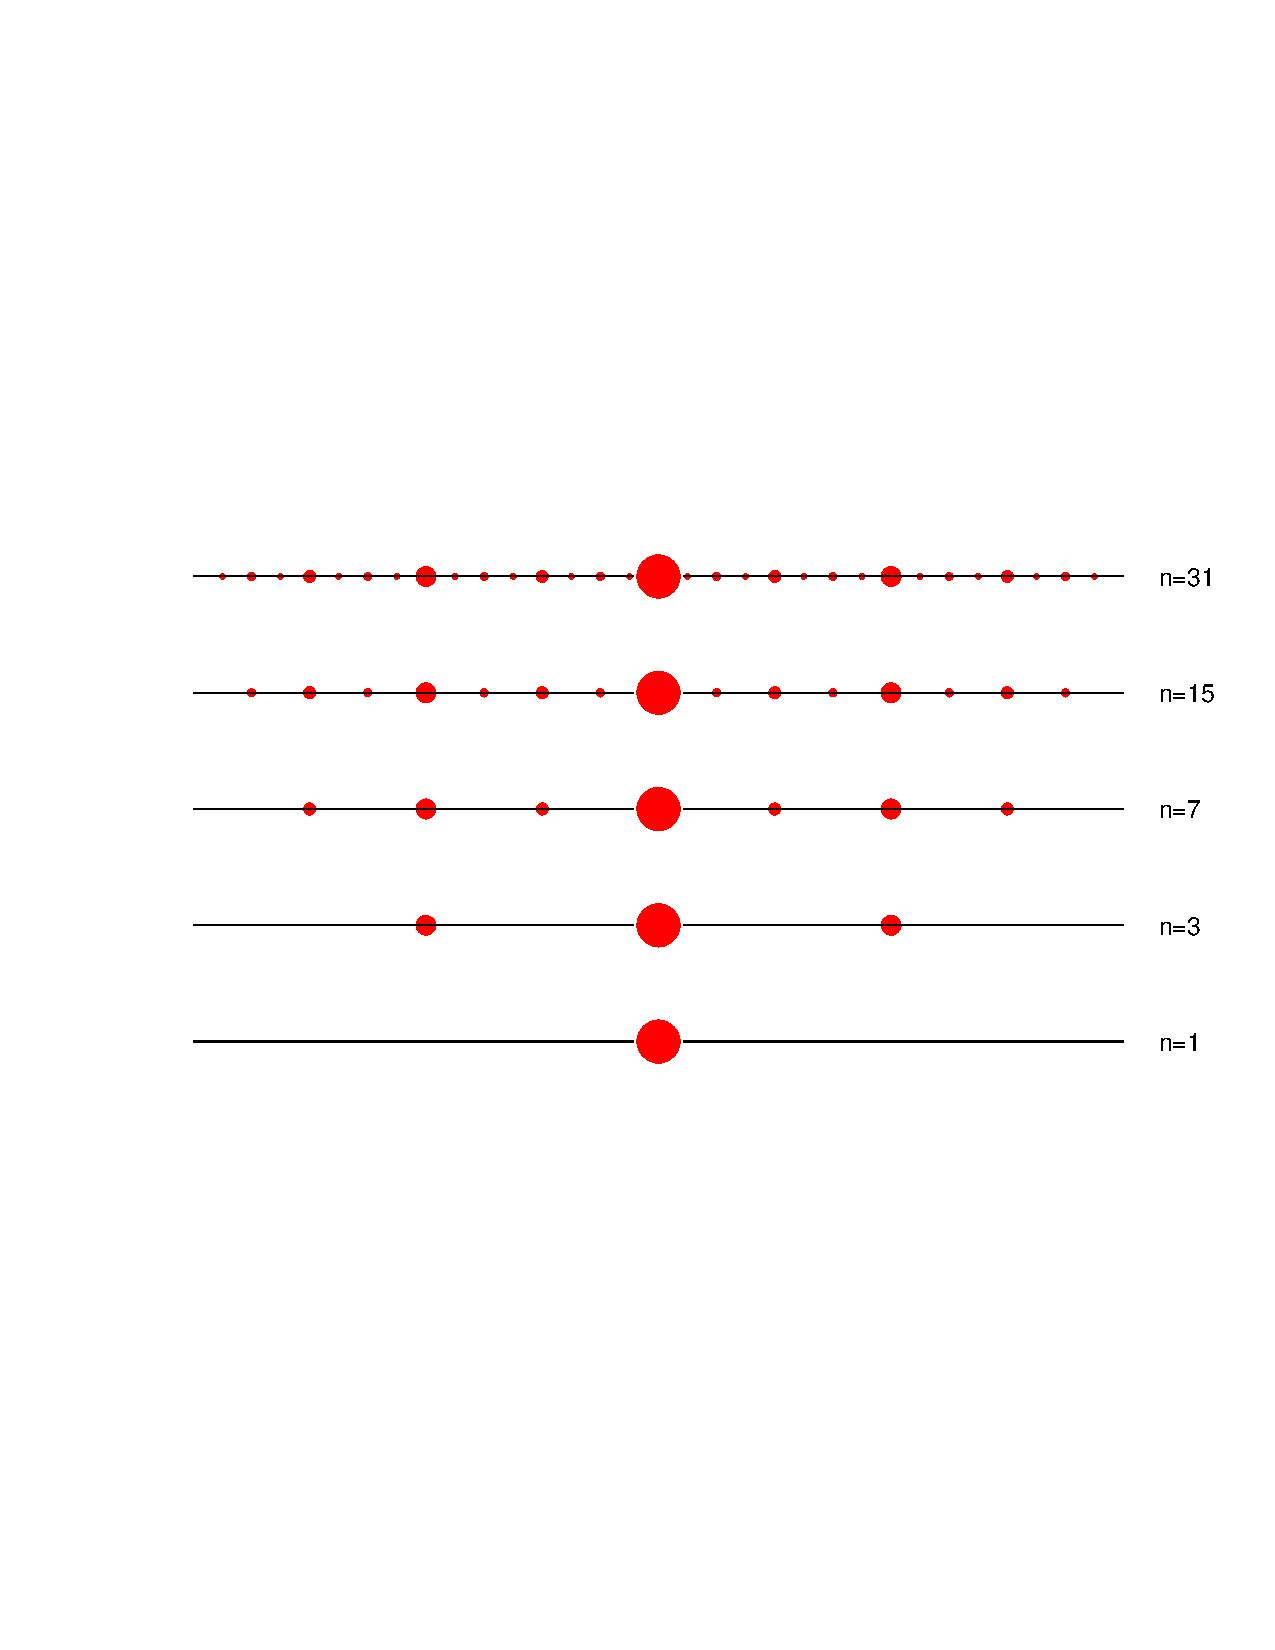
\includegraphics[width=0.5\textwidth]{manygr}
\end{center}
\caption{一维中多个网格
   \label{fig:manygrids}     }
\end{figure}     

对于    $k=1:J$    ,与    \eqref{FEMh}    中定义的有限元空间    $V_h$    类似,我们定义与网格    $\mathcal T_k$    相关联的有限元空间    $V_k$    ,以获得嵌套的有限元空间序列,如下所示:
   \begin{equation}\label{nested_M}
V_1\subset\ldots\subset V_k\subset\ldots\subset V_J.
\end{equation}     

经典的 V 循环几何多重网格方法只是以以下设置递归应用算法~   \ref{alg:two-level}   :
   \begin{enumerate}

   \item      $V_k=V_k$   ;   \item      $A_k: V_k\mapsto V_k$    由    $$
(A_ku_k,v_k)=a(u_k,v_k), \quad u_k,v_k\in V_k;
$$    定义   \item      $\imath_{k-1}^k: V_{k-1}\mapsto V_k$    是包含运算符;   \item      $R_k: V_k\mapsto V_k$    对应高斯-赛德尔等平滑方法。  \end{enumerate}     

   \subsubsection\*{代数设置  }     

方程    \ref{Auf-h}    可以称为有限元方程的算子形式。为了得到向量和矩阵形式的方程,我们使用    $V_h$    
   \begin{equation}
  \label{Mh-basis}
\phi_i(x)=\left \{ \begin{array}{cl}
\frac{x-x_{i-1}}{h}, & x\in[x_{i-1},x_i]; \\ 
\frac{x_{i+1}-x}{h}, & x\in[x_{i},x_{i+1}]; \\ 
0 &\mbox{elsewhere}.
\end{array}\right.
\end{equation}    的节点基函数  

在每个级别上,与    \eqref{Mh-basis}    类似,我们可以为有限元空间    $V_k$    引入一组节点基函数,记为    $ \{ \phi_i^{(k)}: i=1:N_k \} $    。
   \begin{figure}[!htb]
\begin{center}
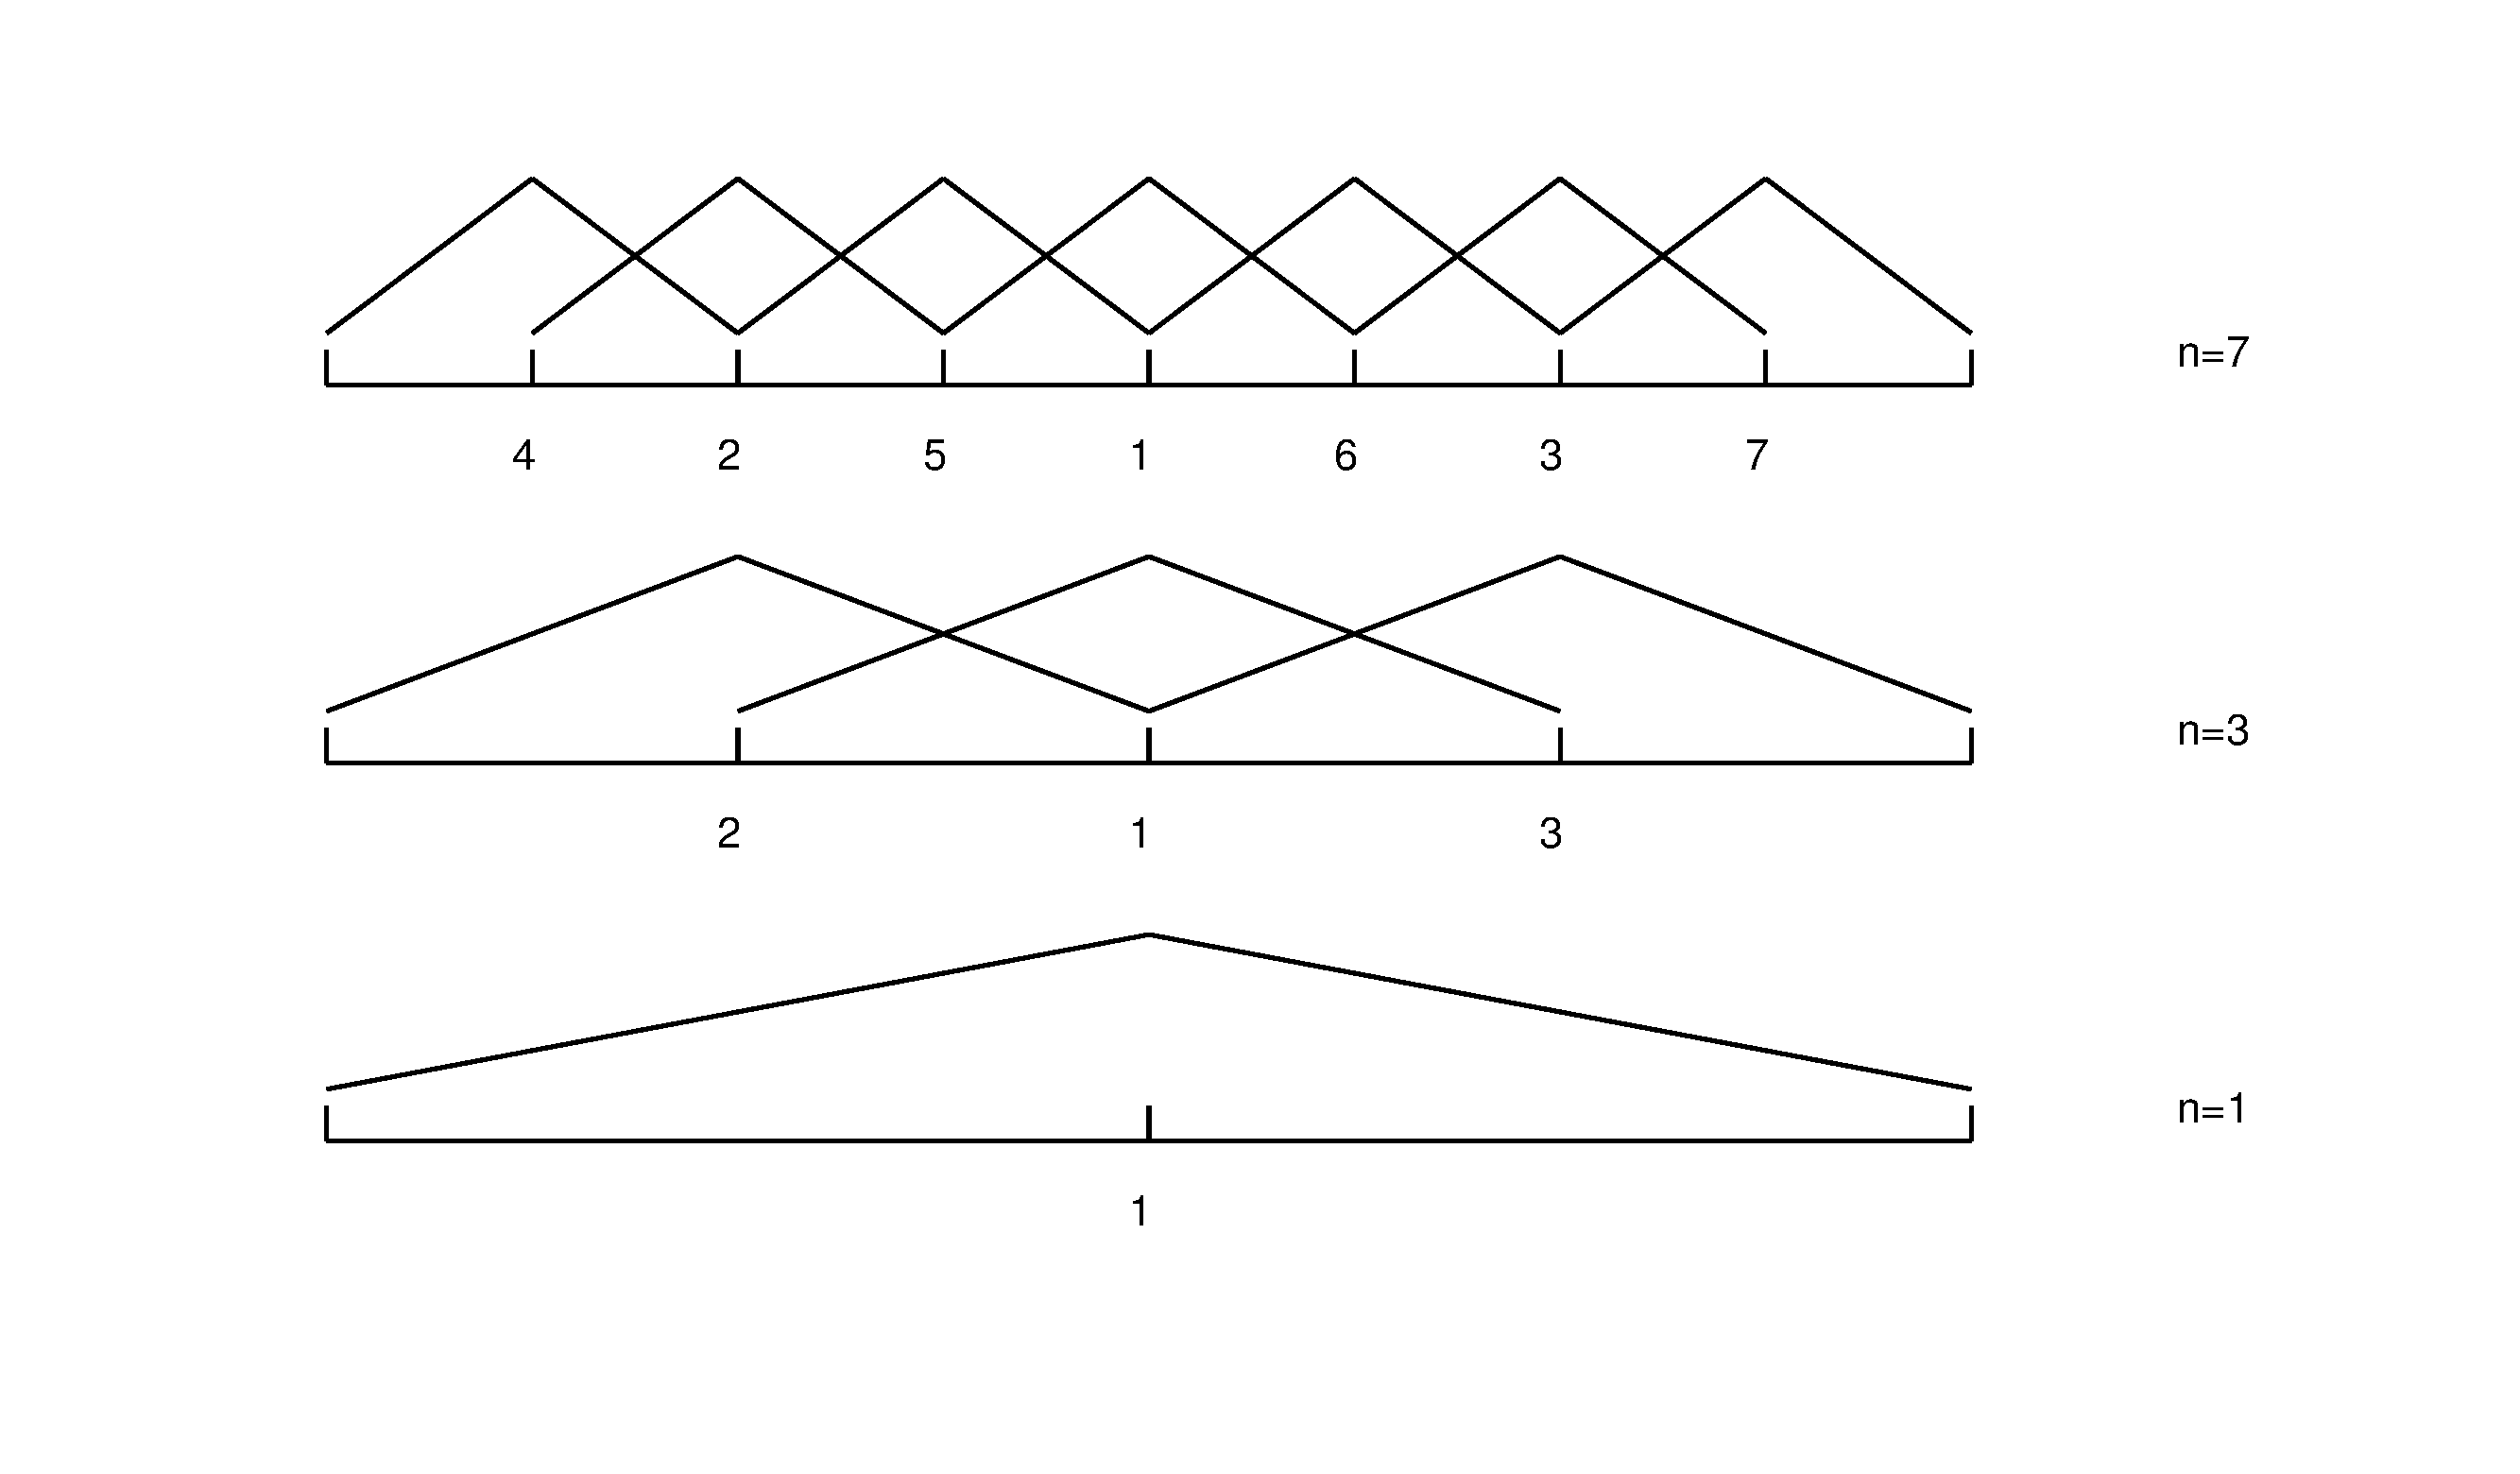
\includegraphics[width=\textwidth]{figures/1dbases}
\end{center}
\caption{每个级别的 1D 节点基函数
   \label{20150914_add1}     }
\end{figure}     

每个    $v\in V_k$    都可以唯一地写成以下基函数的线性组合
   \begin{equation}
    v=\xi_1\phi_1^{(k)}+\xi_2\phi_2^{(k)}+\cdots +\xi_{N_k}\phi_{N_k}^{(k)}.
\end{equation}    这给出了从    $V_k$    到    $\mathbb R^{N_k}$    的同构,它将    $v\in V_k$    映射到    $\mu \in \mathbb R^{N_k}$    ,如下所示
   \begin{equation}
    v=\xi_1\phi_1^{(k)}+\xi_2\phi_2^{(k)}+\cdots +
\xi_{N_k}\phi_{N_k}^{(k)} \longrightarrow \mu=\begin{pmatrix}
        \xi_1 \\ 
        \xi_2 \\ 
        \vdots \\ 
        \xi_{N_k} \\ 
    \end{pmatrix}.
\end{equation}    
   $\mu$    称为    $v$    的矩阵表示。回想一下之前在    \S       \ref{sec:fem}    中的讨论,给出了在    \eqref{Mh-basis}    中定义的    $V_h$    的基础,   \eqref{vph}    等同于    \eqref{axb}    中的线性系统方程。  

我们引入辅助空间    $V_k:=\mathbb R^{N_k}$    。  

从    $V_k$    到    $V_{k+1}$    的转换算子    $P_{k}^{k+1}$    是    $\mathbb R^{N_{k+1}\times N_k}$    中的一个矩阵,并且满足 
   \begin{equation}\label{basis-representation}
    (\phi_1^{(k)} \cdots \phi_{N_k}^{(k)})=(\phi_1^{(k+1)} \cdots \phi_{N_{k+1}}^{(k+1)})\imath_{k}^{k+1}.
\end{equation}    对于我们现在考虑的特殊一维问题,对于    $k=1, 2, \dots, J-1$    我们有 
   \begin{equation}\label{gmg-basis-1d}
    \phi_{j}^{(k)}=\frac12\phi_{2j-1}^{(k+1)}+\phi_{2j}^{(k+1)}+\frac12\phi_{2j+1}^{(k+1)},
\end{equation}    编码此关系的矩阵是
   \begin{equation}\label{p-gmg-1d}
    P_{k}^{k+1} =\begin{pmatrix}
        \frac{1}{2} & & & & \\ 
        1 & & & \\ 
        \frac{1}{2} & \frac{1}{2} & & & \\ 
        & 1 & &  \\ 
        & \frac{1}{2} & \frac{1}{2} & \\ 
        & & 1 & & \\  
        & & \frac{1}{2} & & \\  
        & & & \ddots &\frac{1}{2} \\ 
        & & & &  1 \\ 
        & & & &  \frac{1}{2} \\ 
    \end{pmatrix}.
\end{equation}    经典的    $V$    循环 AMG 方法遵循以下设置,简单地递归应用算法~    \ref{alg:two-level}   :
   \begin{enumerate}[1.]

    \item      $V_k=\mathbb R^{N_k}$   ;   \item      $A_k\in \mathbb R^{N_k\times N_k}: V_k\mapsto V_k$    由    $$
            (A_k)_{ij}= a(\phi_{i}^{(k)}, \phi_{j}^{(k)}), \quad 1\le i, j\le N_k;
        $$    定义   \item      $P_{k-1}^k: V_{k-1}\mapsto V_k$    是    $\mathbb R^{N_{k+1}\times N_{k}}$    中由    \eqref{basis-representation}    定义的矩阵;   \item      $R_k: V_k\mapsto V_k$    对应高斯-赛德尔等平滑方法。  \end{enumerate}    只要我们有多级网格和每级相应的有限元空间,就可以获得针对二维和三维问题的类似多重网格算法。  

   \subsection{从 GMG 获取 AMG  }       \label{s:amg-from-gmg}     

将 GMG 扩展到 AMG 的第一个障碍是 GMG 中使用的几何信息。但仔细检查 GMG 会发现,GMG 方法仅依赖于以下两个主要成分:
   \begin{enumerate}[1.]

   \item   最细网格对应的刚度矩阵;   \item   各层的延长矩阵。  \end{enumerate}    一旦给出了所有延长矩阵,则所有较粗级别的刚度矩阵由以下公式给出
   \begin{equation}\label{galerkin-cgm}
A_{k}=P_{k}^TAP_{k},\quad  k=J-1, J-2, \ldots 1, \quad P_k =\prod_{j=k}^{J-1} P_{j}^{j+1}.
\end{equation}    当然,每个级别也需要一个平滑器,但可以考虑其定义,目前纯粹是代数的。  

由于最精细网格上的刚度矩阵在任何给定应用中始终可用,因此唯一剩下的就是延展矩阵。我们现在将使用线性有限元方法的示例来讨论延展矩阵与几何信息之间的关系。两个观察结果最为相关:
   \begin{description}   \item    [观察 1] 延长矩阵仅取决于与底层网格相关的自然图,而不取决于网格点的坐标。
   \item    [观察 2] 底层网格的图与刚度矩阵的邻接图非常接近。  \end{description}     

基于以上讨论,粗略地说,我们本质上可以仅利用刚度矩阵提供的代数和图形信息来恢复对应于拉普拉斯方程连续线性有限元离散化的刚度矩阵的几何多重网格方法。
   \begin{enumerate}[1.]

   \item   形成刚度矩阵    $A$    的邻接图    $\mathcal G(A)$    ;   \item   使    $\mathcal G(A)$    粗化。  \end{enumerate}     

作为一个说明性示例,让我们考虑与具有双线性元素的平方域上的拉普拉斯方程离散化相对应的刚度矩阵。众所周知,
   \cite{2002CiarletP-aa}    ,在这种情况下的刚度矩阵与 9 点有限差分模板    \eqref{9-point}    的缩放矩阵相同。相应的邻接图(如图~    \ref{gmg}    右侧所示)比图~    \ref{gmg}    左侧所示的网格图更密集(具有更多边)。其边集包括形成网格的每个正方形的对角线。
   \begin{figure}[!htb]
\centering
    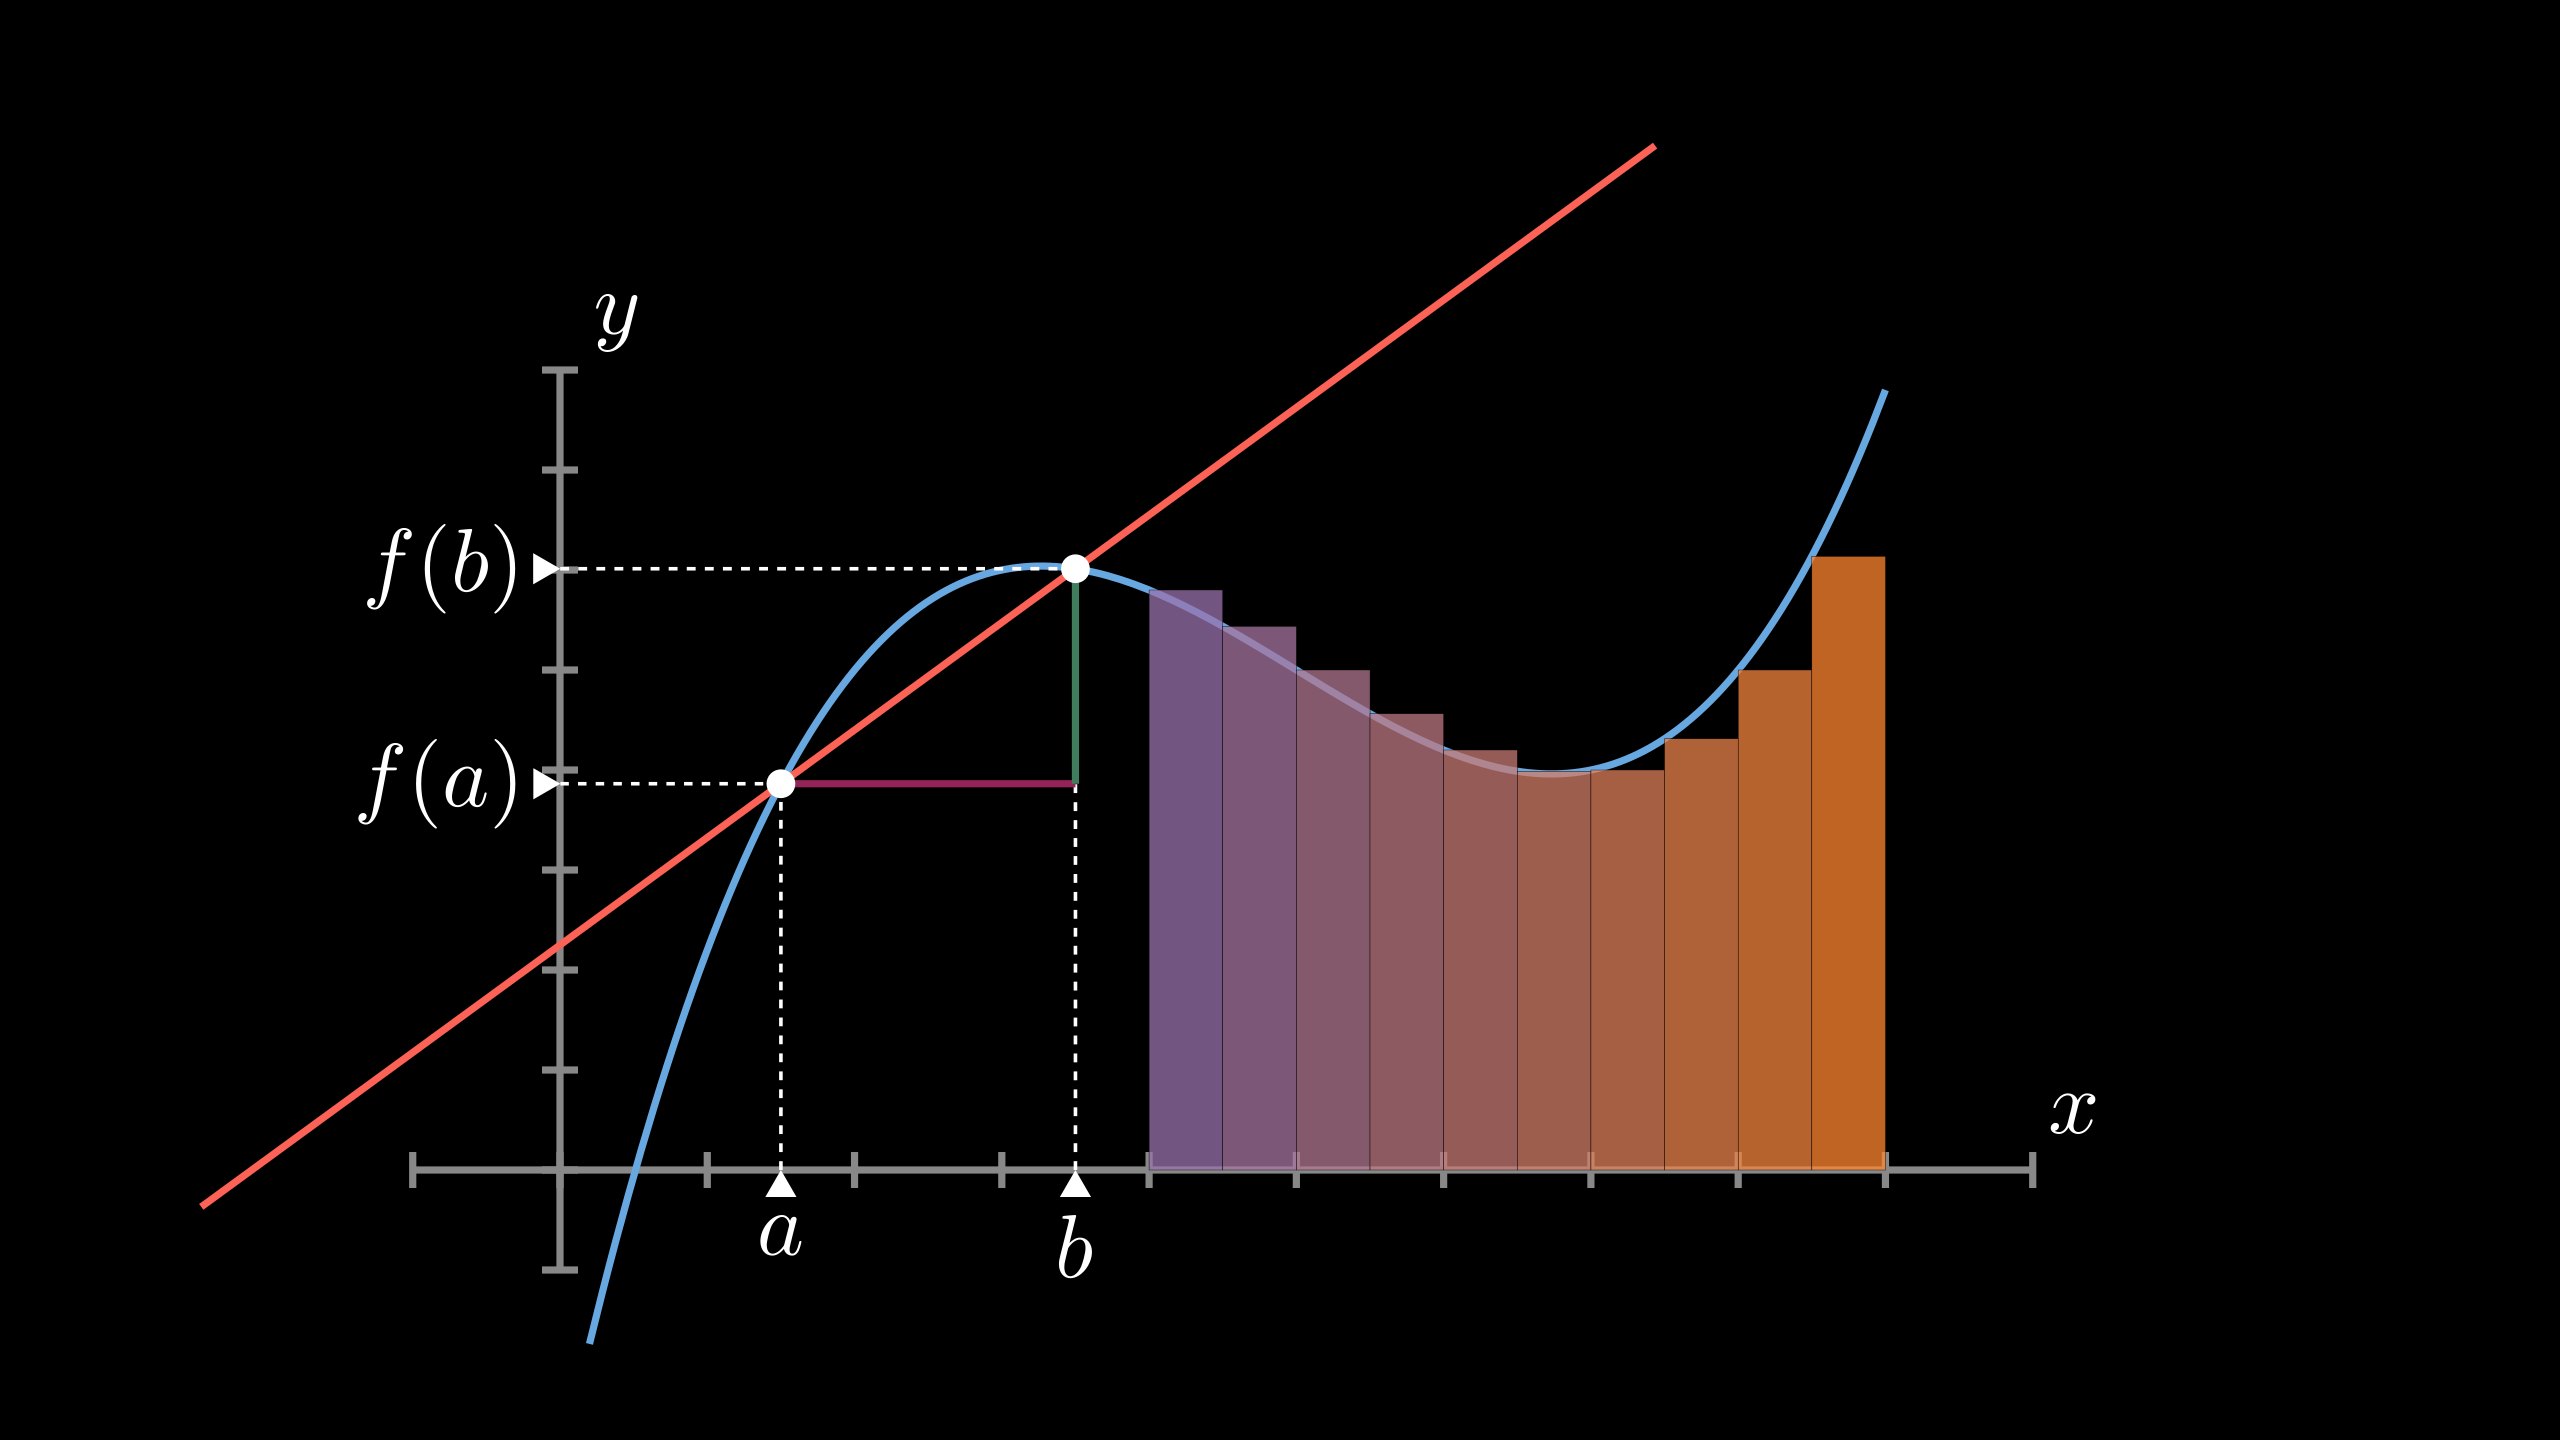
\includegraphics[width=1.0\textwidth]{graph}
\caption{   $6\times 6$    均匀网格(左)、5 点有限差分模板对应的矩阵图(中)和 9 点有限差分模板对应的矩阵图(右)  }
\label{gmg}
\end{figure}    对于延长/插值矩阵的构造,我们回想一下,延长矩阵给出了大小为    $2h$    的网格上的粗网格基函数相对于大小为    $h$    的网格上的细网格基的展开系数。这个矩阵的局部形式如下:
   \begin{eqnarray*}
  [(P_{2h}^h)^T]_i=
\begin{pmatrix}
  \frac{1}{4} &\frac{1}{2} &\frac{1}{4} \\ 
  \frac{1}{2} & 1 & \frac{1}{2} \\ 
 \frac{1}{4} & \frac{1}{2} &\frac{1}{4}
\end{pmatrix}.
\end{eqnarray*}    这个矩阵通常被称为“延长模板”,它以紧凑的形式显示了粗网格基函数展开中的系数。在中心我们有系数    $1$    ,它位于与粗网格顶点相关的细网格基函数前面。其余条目对应于展开中细网格基函数前面的系数。  

在规则细化的三角网格上,我们有一个类似的情况。我们参考~   \S       \ref{sc:connection}    了解有关在这种情况下粗网格自由度选择的详细信息。延长和限制矩阵仅取决于此图的拓扑结构。类似的观察导致了 AMG 的发展:如果几何坐标未知,则需要不同的方法来构建粗空间,从而导致 AMG 算法的不同变体。  

   \subsection{从 AMG 获取 GMG  }       \label{s:gmg-from-amg}    在本节中,我们使用    \S       \ref{sec:unifiedAMG}    中的统一理论从 AMG 获得 GMG。所需的主要成分是空间    $V_j$    ,运算符    $\Pi_j$    ,    $A_j$    ,    $D_j$    和粗空间    $V_j^c$    。  

我们现在考虑为    \eqref{Model0}   (或变分公式
   \eqref{Vari}    )构建一个两级几何多重网格方法。假设我们有两个网格:一个细网格    $\mathcal T_h$    和一个粗网格    $\mathcal T_H$    。在每个网格上,我们分别定义一个线性有限元空间    $V_h$    和    $V_H$   ,节点基函数为
   $ \{ \phi_j^h \} $    和    $ \{ \phi_j^H \} $    ,我们考虑域    $\Omega$    的以下分区:
   \begin{equation}
  \overline{\Omega}=\bigcup_{j=1}^J\overline{\Omega}_j, \text{ with } \overline{\Omega}_j=\operatorname{supp}(\phi_j^H).
\end{equation}     

然后我们将    $V_j$    定义为 
   \begin{equation}
    V_j :=  \{ \chi_jv: v\in V_h \} ,
\end{equation}    其中    $\chi_j$    是    $\Omega_j$    的特征函数。我们注意到    $V_j$    不是    $H^1(\Omega)$    的子空间。算子    $\Pi_j: V_j\mapsto V_h$    定义如下:
   \begin{equation}\label{pi-gamg}
    \Pi_j v_j: = I_h(\phi_j^H v_j), \quad \forall v_j\in V_j,\quad j=1,\ldots,J,
\end{equation}    其中    $I_h$    是细网格上的节点插值算子。这里我们注意到    $\phi_j^H v_j$    在    $\Omega$    中是连续的。我们注意到,根据定义,   $\phi^{H}_j \chi_j = \phi^{H}_j$    在
   $\Omega$    上,这意味着恒等式
   $$
\sum_{j=1}^J \Pi_j \chi_j v = I_h\left(\sum_{j=1}^J\phi_j^H\chi_j
  v\right)
= I_h\left(\sum_{j=1}^J\phi_j^Hv\right)
=I_h(v)=v,
$$    以及因此
   $$
\sum_{j=1}^J \Pi_j \chi_j =\mathrm{Id}. 
$$     

算子    $A_j: V_j\mapsto V_j'$    是双线性形式    $a(\cdot, \cdot)$    的局部限制,即
   \begin{equation}\label{gmg-Aj}
    (A_j u_j, v_j): = a(u_j, v_j)_{\Omega_j} = \int_{\Omega_j}\alpha(x)\nabla u_j\cdot \nabla v_j, \quad u_j, v_j\in V_j
\end{equation}     

下面的估计告诉我们,   $A_j$    满足
   \eqref{sum_Aj}    分解为    $v=\sum_{j=1}^J\Pi_jv_j$    ,其中    $v_j=\chi_jv$    :
   $$
    \sum_{j=1}^{m_c}\|v_j\|_{A_j}^2  =  \sum_{j=1}^{m_c} a(v, v)_{\Omega_j}\le C_1\|v\|_A^2,
$$    ,其中    $C_1$    取决于    $\Omega_j$    的重叠次数。  

我们选择    $D: V \mapsto V'$   ,使用细网格基函数如下 
   \begin{equation}
    (D \phi_i^h, \phi_j^h): = a(\phi_i^h, \phi_j^h)\delta_{ij}, \quad 1\le i, j\le n,
\end{equation}    和
   \begin{equation}\label{duv}
    (D u, v): = \sum_{j=1}^na(\phi_j^h, \phi_j^h)u_jv_j, \quad u, v\in V. 
\end{equation}    请注意,   $(D\cdot, \cdot)$    是    $V$    的内积,它会产生范数    $\|\cdot\|_D$    。  

在上述定义中,   $D$    的矩阵表示是    $A$    的矩阵表示的对角线。类似地,我们可以使用    $V_j$    的基函数定义    $D_j :V_j\mapsto V_j'$   。  

通过简单的缩放参数,我们得到 
   \begin{equation*}
    \|v\|_0^2 \eqqsim h^d\|v\|_{\ell^2}^2.
\end{equation*}    从    \eqref{duv}    ,使用逆不等式,我们得到
   \begin{equation*}
    \|v\|_D^2\lesssim h^{-2}\sum_{j=1}^n\|\phi_j^h\|_0^2v_j^2\eqqsim h^{d-2}\|v\|_{\ell^2}^2\eqqsim h^{-2}\|v\|_0^2.
\end{equation*}    我们还有
   \begin{equation*}
    \|I_hv\|_0^2\eqqsim  h^d\|I_hv\|_{\ell^2}^2 = h^d\|v\|_{l^2}^2\eqqsim \|v\|_0^2.
\end{equation*}    假设〜   \ref{assm:D_j}    然后可以通过以下内容验证
   \begin{eqnarray*}
    \|\sum_{j=1}^{J}\Pi_jv_j\|_D^2 &\lesssim & h^{-2}\|\sum_{j=1}^J\Pi_jv_j\|_0^2 =h^{-2}\|I_h\left(\sum_{j=1}^J\phi_j^Hv_j\right)\|_0^2  \\ 
    &\eqqsim&h^{-2}\|\sum_{j=1}^J\phi_j^Hv_j\|_0^2 =h^{-2}\sum_{i,j=1}^{J}\int_{\Omega}\phi_i^Hv_i\phi_j^Hv_j \\ 
    &\le & h^{-2}\sum_{i,j=1}^{J}\|\phi_i^H\|_{\infty}\|\phi_j^H\|_{\infty}\int_{\Omega}v_iv_j\le h^{-2}\sum_{i, j=1}^{J}\int_{\Omega_i\bigcap\Omega_j}v_iv_j \\ 
    &\le &\co\sum_{j=1}^{J}h^{-2}\int_{\Omega_j}|v_j|^2\lesssim \co\sum_{j=1}^{J}\|v_j\|_{D_j}^2.
\end{eqnarray*}    根据    $A_j$    的定义,   $A_j$    的核由    $V_j$    中的所有常数函数组成,我们选择    $V_j^c$    作为    $\Omega_j$    上常数函数的一维空间。然后
   \begin{equation}
    \mu_j(V_j^c)=\lambda_j^{(2)},
\end{equation}    其中    $\lambda_j^{(2)}$    是算子    $D_j^{-1}A_j$    的第二小特征值。  

全局粗空间    $V_c$    的定义如    \eqref{V_c}    所示。注意,在这种情况下,由定义很容易证明,由    \eqref{V_c}    构造的粗空间    $V_c$    实际上与    $V_H$    相同,即
   \begin{equation}
    V_c=\operatorname{span} \{ \phi_j^H: j=1, \dots, J \} .
\end{equation}    根据定理~    \ref{thm:two-level-conv}    ,此两级几何多重网格方法的收敛速度取决于
   $\min_j(\lambda_j^{(2)})$    。如果庞加莱  { 数学家协会   }  不等式对每个    $V_j$    都成立,即
   \begin{equation}
    \inf_{v_c\in V_j^c} \|v-v_c\|_{D_j}^2\le c_j\|v\|_{A_j}^2, \quad \forall v\in V_j,
\end{equation}    且    $c_j$    为常数,则两级几何多重网格方法均匀收敛。  


 
   

   \subsection{Spectral AMG    $e$   :基于几何的 AMG  }       \label{s:AMGe}    我们现在考虑基于元素的 AMG 方法,并定义在 
   \S       \ref{sec:unifiedAMG}    中的一般结果中适应这些方法所需的成分。AMG    $e$    方法的代数性较低,因为它们假设底层网格并使用元素局部刚度矩阵来定义插值算子。在 AMG    $e$    设置中,假设我们知道    $n\times n$    矩阵    $A$    的分解,
   \begin{equation}
    A=\sum_{\tau\in \mathcal T}\tilde A_{\tau},
\end{equation}    其中,   $\mathcal T$    是用于离散化问题的有限元集,对于每个元素    $\tau\in \mathcal T$    ,   $\tilde
A_\tau$    是局部刚度矩阵    $A_{\tau}$    在    $\tau$    上的零扩展(对称正半定)。  

为了在    \S       \ref{sec:unifiedAMG}    中定义    $V_j$    、    $D_j$    、    $A_j$    和    $\Pi_j$    (对应于 AMG    $e$    ),我们将域    $\Omega$    划分为不相交的子域    $\Omega_1, \dots, \Omega_J$    。每个子域都是元素的集合,以及    $\bar \Omega =\bigcup_{j=1}^J\bar \Omega_j$    。对于每个子域    $\Omega_j$    ,我们引入截止算子    $\chi_j: V\mapsto V_j$    ,其对    $v\in V$    的作用定义为 
   \begin{equation}\label{cutoff}
    (\chi_jv)(x):= \begin{cases}
        v(x), & \text{ if } x\in \bar \Omega_j, \\ 
        0, & \text{ if } x\notin \bar \Omega_j.
    \end{cases}
\end{equation}     

然后我们通过以下公式定义空间    $V_j$   

   \begin{equation}
    V_j: = \chi_j V.
\end{equation}   

   $A_j$    通过将    $\Omega_j$    中所有相关元素的刚度矩阵相加来定义,即

   \begin{equation}
    A_j:=\sum_{\tau\subset\Omega_j}\tilde A_{\tau}.
\end{equation}    显然,   $A_j$    是对称正半定的。很容易验证    \eqref{sum_Aj}    成立。事实上,我们有以下方程

   \begin{equation}
    \sum_{j=1}^J\|\chi_jv\|_{A_j}^2 = \sum_{j=1}^J a(v, v)_{\Omega_j} = \sum_{\tau\in \mathcal T} a(v, v)_{\tau} =\|v\|_A^2.
\end{equation}     

如果我们用    $D$    表示    $A$    的对角线,则    $D_j$    是一个对角矩阵,定义如下
   \begin{equation}
    [D_j]_{ii}: = \begin{cases}
        D_{ii}, & \text{ if } i\in \Omega_j, \\ 
        0, & \text{ if } i\notin \Omega_j.
    \end{cases}
\end{equation}    运算符    $\Pi_j$    由定义为
   \begin{equation}
    [\Pi_j]_{ii}: = \begin{cases}
        [A_j]_{ii}/[A]_{ii}, & \text{ if } i\in \Omega_j, \\ 
        0, & \text{ if } i\notin \Omega_j.
    \end{cases}
\end{equation}    的对角矩阵提供。请注意,如果    $i$    是    $\Omega_j$    的内部点,则    $[\Pi_j]_{ii}=1$    。   \eqref{assm:D_j}    在引理~    \ref{lem:Dj}    中得到验证。  

在每个局部空间    $V_j$    上,谱 AMG    $e$    在局部选择“最佳”粗空间    $V_j^c$   ,即    $D_j^{-1}A_j$    的特征向量所构成的子空间,该子空间属于其    $m_j^c$    最小特征值。然后,全局粗空间由    \eqref{V_c}    定义。  

根据抽象收敛定理 (Theorem~    \ref{thm:two-level-convergence}    ),两级谱 AMG    $e$    的收敛速度取决于每个    $m_j^c+1$    上    $D_j^{-1}A_j$    的最小特征值的最小值,更确切地说,取决于    \begin{equation*}
    \|E\|_A\le 1-\frac{\mu_c}{C_{p,1}C_{p,2}},
\end{equation*}    和    $\mu_c=\min_{1\le j\le J} \mu_{m_j^c+1}^{(j)}$    。  

   \subsection{书目注释  }    
GMG 方法的主要思想首先由 Fedorenko~    \cite{1961FedorenkoR-aa,1964FedorenkoR-aa}    和 Bahvalov~    \cite{1966BahvalovN-aa}    的开创性工作展示。使用群松弛方法的类似思想可以追溯到 20 世纪 40 年代 Southwell 的工作~    \cite{1940SouthwellR-aa,1946SouthwellR-aa}    。真正的多重网格方法的第一个描述出现在 Brandt 的开创性工作    \cite{1973BrandtA-aa}    中。多层方法的进一步发展是由 Brandt~    \cite{1977BrandtA-aa}    和 Hackbusch
   \cite{1977HackbuschW-aa,1978HackbuschW-aa}    进行的。这些工作引起了计算数学和工程界的广泛关注。 Nicolaides~    \cite{1975NicolaidesR-aa,1977NicolaidesR-aa}    、Bank 和 Dupont~    \cite{1980BankR_DupontT-aa}    、Braess 和 Hackbush~    \cite{1983BraessD_HackbuschW-aa}    、Bramble 和 Pasciak~    \cite{bramble1987new}    、Bramble、Pasciak 和 Xu~    \cite{bramble1990parallel,1991BrambleJ_PasciakJ_XuJ-aa}    、Bramble、Pasciak、Wang 和 Xu    \cite{1991BrambleJ_PasciakJ_WangJ_XuJ-ac}    、Xu    \cite{1992XuJ-aa}    等在多重网格方法的收敛性分析方面取得了进展。  

BoxMG~    \cite{1982DendyJ-ab,1983DendyJ-aa}    是一种使用几何细化网格并使用代数技术定义插值的方法。我们参考~    \cite{1982DendyJ-ab,1983DendyJ-aa}    、
   \cite{1990ZeeuwP-aa}    了解详细信息,并参考~    \cite{2012MacLachlanS_MoultonJ_ChartierT-aa}    了解 BoxMG 与经典 AMG 之间等价性的结果。  

基于元素的 AMG 方法,由于它们假设底层网格并使用元素刚度矩阵来定义插值算子,因此代数性较低。此类方法包括纯 AMGe、无元素 AMGe、谱 AMGe 和谱聚集,旨在提高有限元问题基于元素的 AMG 的 AMG 稳健性。我们将不同风格的 AMGe 的结果和讨论参考至~    \cite{Jones.J;Vassilevski.P.2001a,Brezina.M;Cleary.A;Falgout.R;Henson.V;Jones.J;Manteuffel.T;McCormick.S;Ruge.J.2001a,Henson.V;Vassilevski.P.2001a,Brezina.M;Falgout.R;MacLachlan.S;Manteuffel.T;McCormick.S;Ruge.J.2006b}    。  

   \section{能量最小 AMG  }       \label{sec:energy-min}    在这里我们考虑用于构建粗化空间的能量最小化算法。虽然这在历史上并不是第一个 AMG 粗化方法,但我们首先关注这项技术,因为它可用于激发大多数其他 AMG 算法。  

   \subsection{能量最小化与迹最小化  }       \label{s:energy-trace}    在下一个定理中,我们为定理~   \ref{t:trace-min}    添加了一个约束,并给出了最优粗空间    $V_c^{\rm opt}$    与能量最小化之间的关系。我们参考    \S       \ref{2-level-theory}    来定义    $P^{\rm opt}$    和    $\mathcal X_{\eta}$    。
   \begin{theorem}[Trace-minimization theorem]   \label{thm:trace-min}    给定    $\eta>0$    ,让    $\mathcal Z_{\eta}$    定义为 
   \begin{equation}
    \label{Z1}
\mathcal Z_\eta=
\bigg \{ 
  P\in\mathbb R^{n\times n_c}:  (Pv,Pv)_{\bar R^{-1}}\ge \eta (v,v),\;\;
  v\in \mathbb R^{n_c}\mbox{ and } P\bm 1=\sqrt{n_c\eta}\zeta_1\bigg \} 
\end{equation}    然后,   $P\in \argmin_{Q\in \mathcal{Z}_\eta}\operatorname{trace}(Q^TAQ)$    如果 
   $$
    P\in \mathcal Z_{\eta} \text{ and } \range(P)=\range(P^{\rm opt}).
$$     \end{theorem}     

设    $\hat P= \bar R^{-\frac{1}{2}}P$    并定义 
   \begin{equation}\label{yeta}
    \mathcal Y_{\eta}=\bigg \{ P\in \mathbb{R}^{n\times n_c}: (Pv, Pv)\ge \eta(v, v), v\in \mathbb{R}^{n_c} \text{ and } P\bm 1=\sqrt{n_c\eta}\hat \zeta_1 \bigg \} ,
\end{equation}    其中    $\hat \zeta_j$    是    $\bar R^{\frac{1}{2}}A\bar R^{\frac{1}{2}}$    的第    $j$    个最小特征值对应的特征向量。很明显,   $\bar R^{\frac{1}{2}}A\bar R^{\frac{1}{2}}$    和    $\bar RA$    具有相同的频谱。定理〜   \ref{thm:trace-min}    可以写成  

   \begin{theorem}   \label{thm:trace-min-2}    给定    $\eta>0$    ,让    $\mathcal Y_{\eta}$    定义为    \eqref{yeta}    。然后,
   $$ 
    P\in \argmin_{Q\in \mathcal{Y}_\eta}\operatorname{trace}(Q^T\bar R^{\frac{1}{2}}A\bar R^{\frac{1}{2}}Q) \text{ if }
    P\in \mathcal Y_{\eta} \text{ and } \range(P)=\range(P^{\rm opt}).
$$     \end{theorem}     


 
   

假设现在我们在    $V$    上有一个双线性形式    $a(\cdot, \cdot)$    ,它是对称的、半正定的,并且有一个内积
   $(\cdot, \cdot)_{\bar R^{-1}}$    在    $V$    上。例如,这里算子    $\bar{R}$    是缩放并行(即连续)子空间校正方法,对应于将    $V$    拆分为
   \[
V = \sum_{i=1}^n\Span \{ \phi_i \} . 
\]    在实践中,   $\bar R$    可以是    $V$    上任何    $A$    范数收敛平滑器的对称化。这里,为简单起见,我们选择    $\bar R= D^{-1}$    。  

我们现在考虑一个有限元空间    $V$   ,其基函数为    $ \{ \phi_j: j=1:n \} $   。令    $P=(p_{ij})\in \mathbb{R}^{n\times n_c}$    满足 
   \begin{equation}\label{phicP}
    (\phi_1^c, \dots, \phi_{n_c}^c) = (\hat \phi_1, \dots, \hat \phi_n)P, \quad \hat \phi_j=\phi_j/\|\phi_j\|_A, \quad j=1:n.
\end{equation}     

用    $ \{ (\mu_j, \zeta_j) \} $    表示    $\bar RA$    和    $\hat \zeta_j= \zeta_j/\|\zeta_j\|_A$    的特征对。然后我们定义 
   \begin{equation}
    X_{\eta} =\bigg \{  (\phi_1^c, \dots, \phi_{n_c}^c): \text{ it satisfies \eqref{phicP} with } P\in \mathcal Y_{\eta}\bigg \} .
\end{equation}     

我们考虑最小化问题
   \begin{equation}\label{min1}
    \min_{(\phi_1^c,\ldots,\phi_{n_c}^c)\in X_{\eta}} \sum_{j=1}^{n_c}\|\phi_j^c\|_A^2
\end{equation}     

我们注意到
   \begin{eqnarray*}
    \sum_{j=1}^{n_c}\|\phi_j^c\|_A^2 &=& \sum_{j=1}^{n_c}a(\phi_j^c,\phi_j^c)=\sum_{j=1}^{n_c}a(\sum_{k=1}^np_{kj}\hat \phi_k,\sum_{l=1}^np_{lj}\hat \phi_l)  \\ 
    & = & \sum_{j=1}^{n_c}\sum_{k=1}^n\sum_{l=1}^np_{kj}a(\hat \phi_k, \hat \phi_l)p_{lj}= \trace(P^TD^{-\frac{1}{2}}\tilde AD^{-\frac{1}{2}} P).
\end{eqnarray*}    然后定理~    \ref{thm:trace-min}    意味着
   \begin{equation}
    \Span \{ \zeta_j, 1\le j\le n_c \} =\Span \{ \phi_j^0, 1\le j\le n_c \} ,  
\end{equation}    其中
   \begin{equation}
    (\phi_1^0, \dots, \phi_{n_c}^0) \in \argmin_{(\phi_1^c, \dots, \phi_{n_c}^c)\in X_{\eta}}\sum_{j=1}^{n_c}\|\phi_j^c\|_A^2.
\end{equation}    在下一节中,我们使用功能设置并提供有关能量最小化基础设计的详细信息。  

   \subsection{AMG 和 Schwarz 方法的能量最小化基础  }       \label{s:energymin-2}    上述讨论促使人们计算能量最小化基作为带约束的全局优化问题的解。这可能会对所提方法的效率产生影响。然而,正如我们稍后在本节中所示,这并不是一个问题,因为优化问题是经过良好调节的,可以有效求解。我们还在下面显示,解决能量最小化问题的基函数在每个粗网格“元素”内是局部谐波的。能量最小化基的这种性质表明,用于在多重网格法中定义粗空间的各种“谐波扩展”技术(参见~    \cite{chan1998agglomeration,Brezina.M;Cleary.A;Falgout.R;Henson.V;Jones.J;Manteuffel.T;McCormick.S;Ruge.J.2001a,Jones.J;Vassilevski.P.2001a}    )与能量最小化算法密切相关。此性质还表明,能量最小化基也可用于具有多尺度性质的问题的数值均质化(参见    \cite{efendiev2000convergence,hou1999convergence}    )。  

我们从给定的一组子域开始描述 
   $\Omega_i$    ,其特性是没有一个子域完全包含在其余子域的并集中。更准确地说,我们有
   \begin{equation}\label{dd}
    \Omega=\bigcup_{i=1}^{n_c}\Omega_i\mbox{ and }
\bar\Omega_i\bigcap\bigg(\bigcup_{j\neq i}\Omega_j\bigg)^c\neq\emptyset,
\end{equation}    ,其中上标    $c$    是标准集补。等效地,在纯代数设置中,当背景中没有函数空间时,我们可以将    $\Omega_i$    设置为与矩阵    $A$    对应的邻接图的顶点子集)。目的是构造    $\mathcal X_\eta$    中的基函数    $ \{ \phi_i^H \} _{i=1}^{n_c}$    ,并附加以下限制:
   $$
{\rm supp}(\phi_i^H)\subset\bar\Omega_i, \quad 1\le i\le n_c.
$$     

我们希望基函数在所有此类函数中具有最小的总能量,即    $ \{ \phi_i^H \} _{i=1}^{J}$    是以下函数的最小值:
   \begin{equation}\label{min}
    \min \sum_{i=1}^{n_c}\|\psi_i\|_A^2 \quad
    \mbox{subject to}\quad \psi_i\in V_i \text{ and } (\psi_1, \dots,
    \psi_{n_c})\in \mathcal X_\eta. 
\end{equation}    这里 
   \begin{equation}
  \label{vj}
V_i= \{ v\in V_h: {\rm supp}(v)\subset \bar\Omega_i \} , \quad 1\le i \le n_c.
\end{equation}    得益于    \eqref{dd}    ,分解    \eqref{VsumVi}    成立,即
   \begin{equation}\label{VsumVi}
    V=\sum_{i=1}^{n_c}V_i.  
\end{equation}     

   \begin{remark}在 AMG 中,最小化问题~    \eqref{min}    以延长矩阵的形式表示如下:查找
   $P\in \mathbb{R}^{n\times n_c}$    使得
   \begin{equation}\label{e:energymin} 
P=\argmin_{Y\in \mathbb{R}^{n\times n_c}}\mathcal{F}(Y), 
\quad Y\bm{1}_{n_c} = \bm{1}_n,\quad \mathcal{F}(Y) = 
\trace(Y^TAY). 
\end{equation}    就向量而言,局部支持意味着    $P$    中每列(或每行)允许有少量非零值。我们注意到,满足上述属性的函数
   $ \{ \phi_i^H \} $    是线性独立的,这是由于    \eqref{dd}    中的第二个假设和~    \eqref{e:energymin}    中的约束。这种线性独立性相当于假设    $P$    是满秩矩阵(即    $\operatorname{rank}(P)=n_c$   )。  \end{remark}     

根据    \eqref{dd}    中的假设,对于每个    $j$    ,存在    $k\in \Omega_j$    ,使得对于所有    $i\neq j$    ,存在    $k\notin \Omega_i$    。我们定义 
   \begin{equation*}
    \mathcal A_j= \{ k\in \Omega_j: k\notin \Omega_i, i\neq j \} , \quad j=1: n_c.
\end{equation*}    如果    $i\neq j$    ,则存在    $\mathcal A_j\cap \mathcal A_i=\emptyset$    。然后我们定义 
   \begin{equation*}
    \mathcal C = \bigcup_{j=1}^{n_c} \mathcal A_j \text{ and } \mathcal F=\Omega\setminus \mathcal C.
\end{equation*}    我们定义    $N_j\in V'$    如下
   \begin{equation*}
    N_j(v)=\frac{1}{|\mathcal A_j|}\sum_{i\in \mathcal A_j}\psi_i(v)=\frac{1}{|\mathcal A_j|}\sum_{i\in \mathcal A_j}v_i, \quad j= 1:n_c.
\end{equation*}    显然,   $ \{ N_j \} _{j=1}^{n_c}$    是线性独立的,并且如果    $\operatorname{supp}(v)\subset \Omega_j$    ,则对于所有    $i\neq j$    ,存在    $N_i(v)=0$    。  

我们定义    $(V')_c\subset V'$    
   \begin{equation*}
    (V')_c=\operatorname{span} \{ N_j: j=1:n_c \} ,
\end{equation*}    和    $V_{hf}\subset V$    
   \begin{equation*}
    V_{hf}= \{ v\in V: (g, v)=0, \forall g\in (V')_c \} .
\end{equation*}     

如果    $ \{ \varphi_j \} _{j=1}^{n_c}$    满足
   \begin{equation*}
    \operatorname{supp}(\varphi_j)\subset \Omega_j \text{ and } \sum_{j=1}^{n_c}\varphi_j =1,
\end{equation*}    则我们有 ``Gramm'' 矩阵    $G=(G_{ij})=(N_j(\varphi_i))=I$    。根据引理~    \ref{lemma:direct-sum}    ,我们有
   \begin{equation*}
    V=V_{hf}\oplus W_c, \quad W_c=\operatorname{span} \{ \varphi_j: j=1:n_c \} .
\end{equation*}     

首先我们来介绍一些符号。我们定义    $A_i$    对每个子空间    $V_i$    的限制为
   \begin{equation}\label{defAi}
(A_iu_i,v_i)=(A u_i,v_i), \quad \forall  \  u_i,v_i\in V_i,  \quad i=1:n_c.
\end{equation}     

让    $Q_i: V'\mapsto V_i'$    成为定义为自然包含    $V_i\subset V$    的伴随的投影:
   $$
\langle Q_i u', v_i\rangle = \langle u', v_i\rangle \quad \forall v_i\in V_i, \;\; u'\in V'.
$$    我们现在定义以下 PSC 类型预处理器(参见    \eqref{PSC}    )
   \begin{equation}\label{T}
    B=\sum_{i=1}^{n_c}A_i^{-1}\imath_i'=
    \sum_{i=1}^{n_c}\imath_iA_i^{-1}\imath_i'.   
\end{equation}    得益于    \eqref{dd}    ,很容易看出算子    $T:V\mapsto
V$    是同构的。  

现在,我们可以陈述并证明本节中的第一个结果。
   \begin{theorem}   \label{thm:theoremA}    最小化问题
   \eqref{min}    有一个唯一解,由
   \begin{equation}\label{phi}
\phi_i^H = A_i^{-1} Q_i B^{-1}1
\end{equation}    满足
   $$
\operatorname{supp}(\phi_i^H)\subset \Omega_i
$$    给出  \end{theorem}    
   \begin{proof}这个结果实际上直接来自定理    \ref{thm:add}    和    $v=1$    。下面我们给出一个不同的证明。然后通过找到以下二次函数的临界点获得:
   $$
    L = \sum_{i=1}^{n_c}\bigg(
\frac{1}{2}\|\phi_i\|_A^2 - \langle\lambda,\phi_i\rangle.
\bigg)
$$    微分该函数可得出
   $$ [{\partial_{\phi_i}} L] \xi_i = (A\phi_i,\xi_i) -
\langle\lambda,\xi_i\rangle,\quad \xi_i\in V_i.
$$    因此临界点    $(\phi_i^H)$    的第    $i$    个分量由以下公式给出
   \begin{equation}\label{crit1}
(\phi_i,\xi_i)_A = \langle\lambda, \xi_i\rangle, 
\quad\forall \xi_i\in V_i, \quad i=1:n_c.
\end{equation}    从上面的等式我们得到
   $$
\phi_i^H= A_i^{-1} Q_i \lambda. 
$$    总结可得出:
   $$
\lambda = B^{-1} 1. 
$$    这给出了    \eqref{phi}    的推导。
显然,这个唯一的临界点    $(\phi_i^H)$    确实是    \eqref{min}    的唯一全局最小化器,它具有凸目标函数和凸约束。  \end{proof}    现在,我们表明构造的基函数是局部离散的 A 谐波。如果
   $$
(w,v)_A=0,\mbox{ for all } v\in V_{h,0}(D)\equiv \{ v\in V_h: {\rm supp}(v)
\subset\bar D \} .
$$    此属性要求定义它所在的“子域”   $D$   ,则我们称函数    $w\in V$    在子域    $D$    上是离散的 a 谐波。下面,我们将从函数空间的角度介绍此类子域。以下考虑的矩阵/向量表示很容易编写。为了定义粗网格元素的类似物(有限元粗网格的类似物),我们首先考虑    $\Omega$    中位于所有    $\Omega_i$    内部的所有点的集合:
   \begin{equation*}
    \omega_0 = \bigg(\bigcup_{i=1}^{n_c}\partial\Omega_i\bigg)^c \bigcap
\Omega.
\end{equation*}    给定    $x\in\omega_0$   ,定义以下函数,其值位于    $ \{ 1,\ldots,n_c \} $    的子集中,该子集是包含    $x$    的子域
   $\Omega_i$    的索引集:
   \begin{equation}\label{Ix}
  I(x)= \{ i: x\in\Omega_i \} .
\end{equation}    为了排除任何歧义,我们假设对于任何    $x\in
\omega_0$   ,集合    $I(x)$    按升序排列。然后我们定义
   \begin{equation}\label{Kx}
K_x =  \{ y\in \omega_0: I(y)=I(x) \} .
\end{equation}    即    $K_x$    是所有包含    $x$    的    $\Omega_i$    的交集(参见图~    \ref{fig:supports}   )。  

以下简单命题将引导我们得出粗网格元素的适当定义。
   \begin{proposition}   \label{prop:kx}    对于 (   \ref{Kx}   ) 中定义的集合    $K_x$   ,我们有
   \begin{itemize}   \item    [(a)]          $K_x=K_y, \quad \Leftrightarrow\quad I(x)=I(y)$          .
   \item    [(b)]          $K_x\cap K_y=\emptyset$          或          $K_x=K_y$          、          $x\in
\omega_0$          、          $y\in \omega_0$          。
   \item    [(c)] 有有限数量的          $m_H$          不同集合          $K_x$          , 
         $x\in \omega_0$          。  \end{itemize}     \end{proposition}   
   \begin{proof}(a) 中的    $(\Rightarrow)$    方向源于    $x\in
K_x=K_y$    ,因此也源于    $I(x)=I(y)$    。另一个方向源于    $K_{x,y}$    的定义。
为了证明 (b),我们假设存在    $z\in \omega_0$    ,使得    $z\in K_x$    和    $z\in K_y$    。   $K_x$    和    $K_y$    的定义则得出    $I(x)=I(y)=I(z)$    。根据 (a),可知    $K_x=K_y$    。这证明了 (b)。
结论 (c) 直接源于 (b)。  \end{proof}     

让    $\mathcal{T}_H$    表示上述命题    \ref{prop:kx}    中 (c) 中    $m_H$    集合的有限集合。我们有
   $$
\omega_0=\bigcup_{x\in \omega_0} K_x=\bigcup_{K\in \mathcal{T}_H} K. 
$$    显然    $\bar\omega_0=\bar\Omega$    ,
   \begin{equation}\label{EK}
\bar\Omega=\bar\omega_0=\overline{\bigcup_{K\in {\mathcal T}_H} K}
=\bigcup_{K\in {\mathcal T}_H} \bar K.
\end{equation}    这意味着    ${\mathcal T}_H$    的集合形成    $\Omega$    的非重叠分区。   ${\mathcal T}_H$    中的每个元素将被称为  {    \it    粗网格元素   }  。  

   \begin{remark}展示这些宏元素在非结构化网格上的样子是很有诱惑力的,在图    \ref{fig:supports}    中,我们描绘了三个这样的支撑以及它们的交点。但让我们指出,我们在此介绍的技术的一个基本特征是粗元素不需要定义  { 它明确地   } ,它们可能具有相当复杂的形状。  \end{remark}    

   \begin{figure}[!htb]
\begin{tabular}{cc}
\includegraphics*[width=2in]{figures/f1ga}
& \includegraphics*[width=2in]{figures/f2ga} \\ 
\includegraphics*[width=2in]{figures/f3ga} &
\includegraphics*[width=2in]{figures/capfga}
\end{tabular}
\caption{   \label{fig:supports}    一块三角网格和三个基函数的支撑。右下图绘制了交叉点。颜色较深的域对应于粗元素,是所有三个支撑的交叉点。颜色较浅的域是两个支撑的交叉点,白色区域对应于无交叉点。  }
\end{figure}     

   \begin{lemma}设    $\lambda=B^{-1}1$    。假设对于上面定义的每个粗元素    $K\in {\mathcal
T}_H$    ,对于    $K$    中支持的所有    $w_K$    ,我们都有    $(\bm 1,w_K)_A = 0$    。然后
   $$
\langle\lambda,\xi\rangle=0,\mbox{ for all } \xi\in V_{h,0}(K).
$$     \end{lemma}    
   \begin{proof}根据定义,对于某些    $y\in \Omega$    有    $K=K_y$    。因此
   $$ 
V_{h,0}(K)=\bigcap_{i\in I(y)} V_i
\mbox{ and } \sum_{i\in I(y)}\phi_i^H(x)=1,
x\in K.
$$    因此,根据 (    \ref{crit1}    ),我们有 
   $$
(\phi_i,\xi)_A = \langle\lambda, \xi\rangle, 
\quad\forall \xi\in V_{h,0}(K)
$$    和 
   $$
\langle\lambda, \xi\rangle= 
\sum_{i\in I(y)} (\phi_i,\xi)_A =(\bm{1},\xi)_A=0.
$$    然后得到所需的结果。  \end{proof}    当粗化对应于几何多重网格和均匀细化时,引理表明    $\lambda=B^{-1}1\in V'$    是相对于粗化元素的离散边
   $\delta$    函数(即
   $\lambda$    围绕    $\partial K$    得到支持)。图    \ref{fig:lambda}    是    $\lambda$    的示例配置文件和基函数    $\Phi_i^H$    。  

   \begin{figure}[!htb]
\centering
\includegraphics*[width=0.4\textwidth]{figures/tinv}\hfill
\includegraphics*[width=0.4\textwidth]{figures/basis7-14}
    \caption{   $\lambda=B^{-1} \boldsymbol{1}$    的轮廓(左)和典型的基函数    $\phi_i^H$   (右)  }
\label{fig:lambda}
\end{figure}    将上述结果与恒等式    \eqref{crit1}    相结合,我们立即得到本节的第二个主要结果。
   \begin{theorem}   \label{thm:harmonic}    每个基函数    $\phi_i^H$    在每个粗元素    $K\in {\mathcal T}_H$    上都是离散的 a-谐波,即
   \begin{equation}\label{harmonic}
(\phi_i^H,v)_A=0,\quad v\in V_{h,0}(K).   
\end{equation}     \end{theorem}    在一个空间维度(   $d=1$   )中,上述结果相当简单,实际上它已经包含在    \cite{Wan.W;Chan.T;Smith.B.1999a}    中。在这种情况下,基函数    $(\phi_i^H)$    类似于 Babu    \v{s}    ka 和 Osborn~    \cite{babuvska1983generalized}    中的广义有限元基函数。  

所有上述文献中的局部谐波特性都是通过  {    \it    构造   }  从  {    \it    本地   }  元素边界获得的。值得注意的是,这里研究的能量最小化基础是更多  {    \it    全局   }  构造的结果,而局部谐波特性是该构造的副产品。  

   \subsection{能量最小化 AMG 收敛  }    我们给出了基于能量最小化的 AMG 两级收敛的证明。  

我们在    \eqref{dd}    中引入的子域    $\Omega_j$    上定义截断算子    $\chi_j$    如下
   \begin{equation*}
    (\chi_j v)(x): = \begin{cases}
        v(x), & \text{if } x\in \bar\Omega_j, \\ 
        0, & \text{if } x\notin \bar\Omega_j.
    \end{cases}
\end{equation*}    然后我们通过
   \begin{equation*}
    W_j:= \chi_j V={\chi_jv,: v\in V}.
\end{equation*}    定义空间    $W_j$    并且很容易验证
   \begin{equation}\label{local-basis}
   \{ \chi_j\phi_i: \operatorname{supp}\phi_i\cap \Omega_j\neq\emptyset \} 
\end{equation}    构成了    $W_j$    的基础。  

算子    $\Pi_j: W_j\mapsto V$    的定义与    \eqref{pi-gamg}    中相同,其中    $\phi_j^H$    是最小化问题    \eqref{min}   (定理~   \ref{thm:theoremA}    中的    \eqref{phi}   )的解。  

然后我们有
   \begin{equation*}
    \sum_{j=1}^{n_c} \Pi_j\chi_j ={\rm Id}
\end{equation*}    事实上,我们有
   \begin{equation*}
    \sum_{j=1}^{n_c}\phi_j^H(x)=\sum_{j: x\in\Omega_j}\phi_j(x)=\sum_{j\in I(x)}\phi_j(x)=1,
\end{equation*}    这意味着身份
   \begin{equation}
    \sum_{j=1}^{n_c} \Pi_j \chi_j v = I_h\left(\sum_{j=1}^{n_c}\phi_j^H\chi_j v\right)=I_h(v)=v,
    \text{ and hence }    \sum_{j=1}^{n_c} \Pi_j \chi_j =\mathrm{Id}. 
\end{equation}     

算子    $A_j: W_j\mapsto W_j'$    是双线性形式    $a(\cdot, \cdot)$    的局部限制,如    \eqref{gmg-Aj}    一样。  

   \eqref{sum_Aj}    满足分解    $v=\sum_{j=1}^{n_c}\Pi_jv_j$    其中    $v_j=\chi_jv\in W_j$    :
   \begin{equation*}
    \sum_{j=1}^{m_c}\|v_j\|_{A_j}^2  =  \sum_{j=1}^{m_c} a(v, v)_{\Omega_j} \le \co \|v\|_A^2
\end{equation*}    其中    $\co$    取决于    $\Omega_j$    的重叠次数。  

我们选择    $D: V \mapsto V'$    使用细网格基函数,如下所示 
   \begin{equation}
    (D \phi_i^h, \phi_j^h): = (A \phi_i^h, \phi_j^h)\delta_{ij}, \quad 1\le i, j\le n.
\end{equation}    请注意,在上面的定义中,   $D$    的矩阵表示是    $A$    的矩阵表示的对角线。类似地,我们可以使用    \eqref{local-basis}    中定义的    $W_j$    的基函数定义    $D_j: W_j\mapsto W_j'$    ,而    $D_j$    的矩阵表示是    $A_j$    的矩阵表示的对角线。众所周知 
   \begin{equation*}
    \|v\|_D^2\eqqsim h^{-2}\|v\|_0^2, \forall v\in V, \text{ and } \|v_j\|_{D_j}^2\eqqsim h^{-2}\|v_j\|_0^2, \forall v_j\in W_j.
\end{equation*}     

   \eqref{assm:D_j}    可以通过以下方式验证
   \begin{eqnarray*}
    \|\sum_{j=1}^{n_c}\Pi_jv_j\|_D^2 &\lesssim &h^{-2}\int_{\Omega}\left(\sum_{j=1}^{n_c}\phi_j^Hv_j\right)^2= h^{-2}\sum_{i,j=1}^{n_c}\int_{\Omega}\phi_i^Hv_i\phi_j^Hv_j \\ 
    &\le & h^{-2}\sum_{i,j=1}^{n_c}\|\phi_i\|_{\infty}\|\phi_j\|_{\infty}\int_{\Omega}v_iv_j \\ 
    &\le & h^{-2}(\max_{1\le j\le n_c}\|\phi_j\|_{\infty})^2\sum_{i, j=1}^{n_c}\int_{\Omega_i\bigcap\Omega_j}v_iv_j \\ 
    &\le &\co(\max_{1\le j\le n_c}\|\phi_j\|_{\infty})^2\sum_{j=1}^{n_c}h^{-2}\int_{\Omega_j}|v_j|^2 \\ 
    &\lesssim &\co(\max_{1\le j\le n_c}\|\phi_j\|_{\infty})^2\sum_{j=1}^{n_c}\|v_j\|_{D_j}^2.
\end{eqnarray*}     

我们选择局部粗空间    $W_j^c\subset W_j$    作为    $\bar\Omega_j$    上的常数函数空间。然后全局粗空间    $V_c$    定义为 
   \begin{equation*}
    V_c:=\sum_{j=1}^{n_c}\Pi_jW_j^c.
\end{equation*}    事实上,对于这种情况,   $V_c$    是    $ \{ \phi_j^H \} $    所跨越的子空间:
   \begin{equation}
    V_c=\operatorname{span} \{ \phi_j^H: j=1, \dots, n_c \} .
\end{equation}     

我们以某种方式选择子域    $\Omega_j$   ,使得 Poincar\'{e} 不等式成立
   \begin{equation*}
    \inf_{v_c\in W_j^c}\|v-v_c\|_0^2\le cd_j^2|v|_1^2,
\end{equation*}    其中    $d_j$    是    $\Omega_j$    的直径,   $c$    是与网格大小和    $\Omega_j$    的大小无关的常数。由于
   \begin{equation*}
    \|v\|_{D_j}^2\eqqsim h^{-2}\|v\|_0^2, \quad  \|v\|_{A_j}^2 \eqqsim |v|_1^2,
\end{equation*}    我们有
   \begin{equation*}
    \inf_{v_c\in W_j^c}\|v-v_c\|_{D_j}^2\le c\left(\frac{d_j}{h}\right)^2\|v\|_{A_j}^2,
\end{equation*}     

结合以上讨论和定理~   \ref{thm:two-level-conv}   ,我们得到
   \begin{theorem}基于能量最小化的两级 AMG 的收敛速度有如下界限:
   \begin{equation}
        \|E\|_A\le 1-\mu,
    \end{equation}    和    $0<\mu<1$    仅取决于子域    $\Omega_j$    的大小和重叠。  \end{theorem}     

   \subsection{书目注释  }    能量最小化似乎包含几种算法:这种最小化的拉格朗日方程在经典 AMG(   \S       \ref{s:classical-amg}   )中近似求解,而函数在平滑聚合(   \S       \ref{s:agmg}   )中近似最小化。  

对于能量最小化方法,我们参考了    \cite{Mandel.J;Brezina.M;Vanek.P.1999a,Wan.W;Chan.T;Smith.B.1999a,chan1998agglomeration,Xu.J;Zikatanov.L.2004a,Brannick.J;Zikatanov.L.2006b}    的作品。一个有趣的事实是,对于规则细化的网格,只要有正确的支持,轨迹(能量)最小化延长会非常接近地恢复粗基,尽管并不完全接近。微小的差异是由于边界的影响,粗网格基函数在图中距离越远,它就越接近分段线性。  

在~   \cite{Wan.W;Chan.T;Smith.B.1999a,wan1998scalable,Mandel.J;Brezina.M;Vanek.P.1999a,Xu.J;Zikatanov.L.2004a}    中报告的大量数值实验表明,能量最小化基础可使许多实际问题(尤其是具有粗糙系数的问题)的二网格和多重网格方法一致收敛。这些方法还为数值均质化提供了框架,并且与~   \cite{1997GrauschopfT_GriebelM_ReglerH-aa}    中的均质化方法和~   \cite{2011LipnikovK_MoultonJ_SvyatskiyD-aa}    中的 M    $^3$    技术相关。  

Van    \v{e}    k、Mandel 和 Brezina 的著作中介绍了代数多重网格法中的“平滑聚合”方法及其理论框架。在粗空间基的构建和基函数的“能量”之间建立了明确的关系。正如在~    \cite{Wan.W;Chan.T;Smith.B.1999a}    和~    \cite{Mandel.J;Brezina.M;Vanek.P.1999a}    中指出的那样,这可以看作是朝着最小化我们上面考虑的二次(能量)函数的方向获得基函数的一个(或几个)步骤。  

在~    \cite{2011OlsonL_SchroderJ_TuminaroR-aa}    中探索了包括长距离能量最小化延长在内的不同稀疏模式,而在~    \cite{2012SchroderJ-aa}    中探索了各向异性问题。  

在~    \cite{2006VassilevskiP_ZikatanovL-aa}    中考虑了保留多个向量的约束能量最小化。在 FE 设置中,当元素刚度矩阵可用时,局部能量最小化提供粗空间,从而导致均匀的两级收敛~    \cite{2006KolevT_VassilevskiP-aa}    。  


 
   

   \section{经典AMG  }       \label{s:classical-amg}    经典 AMG 中的粗空间始终被视为通过延长(插值)矩阵定义的子空间。其维度    $n_c$    是精细空间维度的一小部分。经典 AMG 中流行的插值方案是直接插值、标准插值或多遍插值。此类插值的矩阵表示形式为    $P=\begin{pmatrix}W \\ I \end{pmatrix}$    和    $W\in \mathbb{R}^{n_F\times n_C}$    ,它们可被视为所谓“理想”插值的稀疏近似值    $W=-A_{FF}^{-1}A_{FC}$    ,通常是一个满矩阵。这里,矩阵    $A_{FF}$    是与    $F$    点相对应的矩阵块,而    $A_{FC}$    是与    $C$    点和    $F$    点之间的连接相对应的块。使用~    \S       \ref{sc:connection}    中描述的粗化策略之一,对子集    $F$    和    $C$    中与    $A$    对应的邻接图的顶点进行拆分。  

   \subsection{经典 AMG 的粗糙空间  }       \label{s:idealHL}     

经典 AMG 中的粗化算法使用将对应于    $A$    的图的顶点集    $ \{ 1, 2, \dots, n \} $    拆分为两个不相交的集合
   \begin{equation}\label{e:cf}
    \mathcal C\cup \mathcal F= \{ 1, 2, \dots, n \} , \quad \mathcal C\cap \mathcal F=\emptyset.
\end{equation}    其中    $\mathcal C$    是最大独立集,其独立性相对于在~    \S       \ref{s:strength}    中定义的强度算子    $S$    的图,并且拆分称为“   $C/F$    -拆分”。在~    \S       \ref{s:MIS}    、算法~    \ref{a:MIS}    中引入了一种简单的贪婪    $C/F$    -拆分算法。  

我们假设    $V$    配备一个基础    $ \{ \phi_k \} _{k=1}^n$    ,并且我们让    $n_f=|\mathcal F|$    ,    $n_c=|\mathcal C|$    表示形成    $C/F$    分裂的集合的基数。并非总是如此,但在方便时,我们假设 
   \begin{equation}\label{cf-order}
    \mathcal F= \{ 1,\ldots,n_f \}  \text{ and } \mathcal C= \{ n_f+1,\ldots,n \} .  
\end{equation}    在这种情况下,在
   \eqref{polarVhf}    中定义的高频空间    $V_{hf}$    可以写成
   \begin{equation}\label{Vhf}
V_{hf}=\operatorname{span} \{ \phi_j, j\in \mathcal F \} .
\end{equation}    按照    \S       \ref{sc:connection}    中的步骤,我们首先着手确定一个暂定的粗空间    $W_c$    。一个最简单的选择如下:
   \begin{equation}
  \label{classicalWc}
W_c=\Span  \{ \phi_j, j\in \mathcal C \} .
\end{equation}    显然上述暂定空间满足    \eqref{VhfWc}    ,即
   $$
V=V_{hf}\oplus W_c. 
$$    但    $W_c$    几乎不是低频空间。给定    $W_c$    中的一个基函数    $\phi_{j_k}$    ,我们滤除其高频分量以获得以下粗基函数,
   \begin{equation}
\label{phiHh}
\phi_{k,c}:= (I-\Pi_{hf})\phi_{j_k} = \phi_{j_k} + \sum_{j\notin \mathcal C} p_{jk} \phi_j.  
\end{equation}    这里    $P_{hf}$    是    $(\cdot, \cdot)_A$    在
   $V_{hf}$    上的正交投影。根据    $\Pi_{hf}$    的定义:
   $$
\Pi_{hf}\phi_k= \begin{cases} \phi_k, &\text{ if } k\in \mathcal F, \\ 
-\sum\limits_{j\in \mathcal F}p_{jk}\phi_j, &\text{ if } k\in \mathcal C, \\ 
\end{cases}
$$    其中    $p_{jk}$    满足
   \begin{equation}\label{phf-def}
-\sum\limits_{j\in \mathcal F}p_{jk}(\phi_j, \phi_i)_A = (\phi_k, \phi_i)_A,
\quad \mbox{for all } i\in \mathcal F,\quad k\in \mathcal C.
\end{equation}    在矩阵表示法中,按照    \eqref{cf-order}    给出的顺序,~    \eqref{phf-def}    中方程的矩阵形式为
   \begin{equation}\label{e:harmonic}
A_{FF} W = A_{FC}, \quad \mbox{where}\quad A = 
\begin{pmatrix}
A_{FF} & A_{FC} \\ 
A_{FC}^T & A_{CC}
\end{pmatrix}. 
\end{equation}    这里,   $W_{jk} = p_{jk},\; j\in \mathcal F, \; k\in \mathcal C$    ,其中    $p_{jk}$    是~    \eqref{phf-def}    中给出的系数。  

根据引理    \ref{lem:basis-in-vc}    ,我们有    $S=I-\Pi_{hf}$    。   $V_c$    是    \eqref{phiHh}    中函数的跨度 
   \begin{equation*} 
   V_c = \Span \{ \phi_{k,c} \} _{k=1}^{n_c}= \operatorname{Range}(I-P_{hf}).
 \end{equation*}    我们注意到
   $$
(\phi_{1,c},  \ldots, \phi_{n_c,c})=(\phi_1,\ldots, \phi_{n})
\begin{pmatrix}
  W \\ 
I
\end{pmatrix}.
$$    因此相应的延长矩阵是
   \begin{equation}\label{idealP}
P=\begin{pmatrix}W \\  I\end{pmatrix}, \quad W=-A_{FF}^{-1}A_{FC}.
\end{equation}       \eqref{phiHh}    中给出的函数    $ \{ \phi_{k, H} \} $    构成了
   $V_c$    的基础,类似于拉格朗日有限元的几何多重网格法。我们用    $P^{\rm opt}$    表示    \eqref{idealP}    中定义的延长矩阵,并在下文中将其称为理想插值。  

可以轻松建立以下结果。
   \begin{lemma}如果    $A$    满足    $A \boldsymbol 1=0$    ,则 ~    \eqref{e:harmonic}    的解也满足 ~    \eqref{e:energymin}    中的约束,即
   \(W\boldsymbol 1_{n_c}=\boldsymbol 1_{n_F}\)    。  \end{lemma}     

接下来,我们引入延伸集    $\mathcal P_C$    、
   $$
\mathcal P_C=
\left \{ P\;\big|\; P=
\begin{pmatrix}
  W \\ 
I
\end{pmatrix}
\right \} .
$$    ,并从    \eqref{chi}    和    \S       \ref{sec:energy-min}    中给出的定义中回想一下,
对于某个常数    $\eta> 0$    ,
   $$
\mathcal P_C\subset \eta\mathcal X,
$$    。例如,如果    $\bar R^{-1} \eqqsim D$    ,则    $\eta\eqqsim \max_{1\le j\le n}|D_{jj}|$    ,其中    $D$    是    $A$    的对角线。等效地,   $P\in \mathcal{P}_C$    表示粗网格基础定义为
   \[ \phi_{k,H} = \phi_{j_k} + v_f, \quad j_k\in \mathcal C, \quad v_f\in V_f,
\quad k=1,\ldots,n_c.
 \]    显然,   $\mathcal{P_C}$    的所有元素都是满秩的,并且根据定义,我们也有
   $P^{\rm opt}\in \mathcal{P}_C$    。  

我们有以下定理,表明对应于
   $V^{\rm opt}_c=\range(P^{\rm{opt}})$    的粗网格矩阵具有最小迹。
   \begin{theorem}   \label{t:energymin}    如果我们固定索引集    $\mathcal C$    和粗网格自由度,那么对于    $P^{\rm opt}$   ,我们有
   \begin{equation}\label{first-trace-min}
P^{\rm opt}=\argmin_{P\in \mathcal{P}_C}\trace(P^TAP).
\end{equation}    
此外,如果我们表示    $A_c=(P^{\rm opt})^TAP^{\rm opt}$    ,那么
   \begin{equation}\label{second-trace-min}
    \|v_c\|_{A_c}^2 = \min\left \{ \|v\|^2_A \;\;\bigg|\;\;
\langle \phi_{j_k}',v\rangle=v_{c,k}, \; k=1,\ldots,n_c \right \} 
\end{equation}     \end{theorem}    
   \begin{proof}关系~    \eqref{first-trace-min}    可由以下简单恒等式得出。
   \begin{eqnarray*} 
\trace(A_c) & = &
\sum_{k=1}^{n_c}\|\phi_{k,H}\|_A^2 =
\sum_{k=1}^{n_c}\|(I-P_{hf})\phi_{j_k}\|_A^2  \\  & = &
\sum_{k=1}^{n_c}\min_{v_{k}\in V_{hf}}\|\phi_{j_k}+v_{k}\|_A^2  \\ 
& = &
\min\left \{ \sum_{k=1}^{n_c}\|\phi_{j_k}+v_{k}\|_A^2\;\;\bigg|\;\;
v_{k}\in V_{hf}, \; k=1,\ldots,n_c\right \}  \\  &=&\min_{P\in
\mathcal{P}_C}\trace(P^TAP).
\end{eqnarray*}    
为了证明    \eqref{second-trace-min}    ,我们注意到任何 
   $v\in V$    使得    $\langle\phi_{j_k}',v\rangle=v_{c,k}$    可以写成 
   \begin{equation*}
    v= w_c+v_f, \text{ where }   w_c=\sum_{k=1}^{n_c}v_{c,k}\phi_{j_k}.
\end{equation*}    根据    $P_{hf}$    的定义,我们有    $(I-P_{hf})v_f=0$    和
   $v_c=(I-P_{hf})(v-v_f)=(I-P_{hf})v$    。然后我们有
   \begin{eqnarray*}
 \|v\|_A^2 &=& \|P_{hf}v\|_A^2+\|(I-P_{hf})v\|_A^2 
=\|P_{hf}v\|_A^2+\|v_c\|_{A_c}^2
\ge \|v_c\|_{A_c}^2
\end{eqnarray*}     \end{proof}     

定理~    \ref{t:energymin}    表明最小化器    $P$    满足方程~    \eqref{e:harmonic}    。根据定理~    \ref{t:energymin}    可知,在    $A\bm{1}=0$    的情况下,~    \eqref{e:energymin}    的最小化器和~    \eqref{e:harmonic}    的解是相同的。  


   

   \subsection{理想插值的拟最优性  }     

下面的两级收敛结果是众所周知的(例如参见~
   \cite{2006MacLachlanS_ManteuffelT_McCormickS-aa}    )。
   \begin{theorem}   \label{t:ideal-converges}    对于定义为最小化问题~    \eqref{e:energymin}    的解或等效地~    \eqref{e:harmonic}    的解的    $P^{\rm opt}$   ,具有延长    $P^{\rm opt}$    的两级 AMG 方法以
   $\|E\|_A\le 1-\delta$    的速率收敛,其中    $\delta$    是一个常数,仅取决于对应于
   $A$    的图中顶点的最大度数和选择强连接的阈值    $\theta$   。  \end{theorem}     

   \begin{proof}根据推论~    \ref{c:AHF}    ,我们只需要验证
   $V_{hf}$    由定义~    \ref{def:high-frequencies}    中定义的    $\delta$    -代数高频组成。显然,从    \S       \ref{sec:m-matrix}    中的讨论中,我们可以假设    $A$    是一个
   $M$    -矩阵,所有连接都是强连接。我们考虑对应于    $A$    的图,并回想一下,粗网格自由度集是此图中的最大独立顶点集。根据连接强度的定义,对于任何
   $j\in  \{ 1,\ldots,n \} $    和任何    $i\in N(j)$    ,我们有
   \begin{equation*}
        a_{jj} = \sum_{k\in N_j}-a_{jk}\le |N_j|\max_{k\in N_j}(-a_{jk})\le -\frac{|N_j|}{\theta}a_{ji}
    \end{equation*}    
接下来,对于任何    $j\in F$    ,让    $k_j\in \mathcal C$    使得
   $|a_{k_j, j}|>0$    。这样的    $k_j$    存在,因为
   $C$    顶点集是最大独立集。这种选择不是唯一的,我们只需为每个    $j$    固定一个这样的索引    $k_j$    。使用    \S       \ref{sc:connection}    中的符号,以及    $v\in V_{hf}$    在    $C$    顶点处消失的事实,我们得到
   \begin{eqnarray*}
      \|v\|_{\bar R^{-1}}^2 &\le& 
c^D\|v\|_D^2 = c^D\sum_{j\in F}a_{jj}v_j^2 = c^D\sum_{j\in F}a_{jj}(v_j-v_{k_j})^2 \\ 
                            & \le & c^D\sum_{j\in F}-\frac{|N_j|}{\theta}a_{j,k_j}(v_j-v_{k_j})^2 \\ 
                            &\le &\max_{j}(|N_j|) \frac{c^D}{\theta} \sum_{(i,j)\in \mathcal E}-a_{ij}(v_i-v_j)^2 \\ 
                            &\le & \max_{j}(|N_j|) \frac{c^D}{\theta}\|v\|_A^2.
    \end{eqnarray*}     \end{proof}     

我们注意到,像    $P^{\rm opt}$    这样的插值在实践中并不使用(一维问题可能除外),因为延长矩阵    $P^{\rm opt}$    可能有很多填充并且
   $(P^{\rm opt})^TAP^{\rm opt}$    是密集的。然而,同样重要的是要注意,   $P^{\rm opt}$    的稀疏近似是实践中使用的。因此,构建粗空间中的能量最小化技术可以被看作是用于构建    $V_c^{\rm opt}$    近似的其他 AMG 技术的动机。例如,大多数已知技术近似于~    \S       \ref{s:energymin-2}    中给出的函数    $\mathcal{F}$    的最小化器,方程~    \eqref{e:energymin}   :(1) 在经典 AMG 框架中构建的延长矩阵在由稀疏矩阵组成的    $\mathcal{P}_C$    子集上近似方程~    \eqref{e:harmonic}    的解; (2)在~    \S       \ref{s:energymin-2}    中概述的能量最小化技术和在~    \S       \ref{s:sa}    中考虑的平滑聚合,最小化(近似地)一组稀疏矩阵    $P$    上的粗网格矩阵    $\mathcal{F}(P)$    的迹。  

   \subsection{延拓矩阵   $P$   的构造  }       \label{sec:classicP}     

   \subsubsection{延长  }     

找到问题    \eqref{e:harmonic}    的近似解的一个直观想法是使用一些基本的迭代方法,例如雅可比方法,然后适当地重新调整    $W$    的系数,使其满足    \begin{equation}\label{const_preserv}
     W\boldsymbol 1_{n_c}=\boldsymbol 1_{n_f},
 \end{equation}    并且也符合稀疏模式:
   \begin{equation}\label{sparsity}
     W\in \mathbb{R}_{S}^{n_f\times n_c}.
 \end{equation}    按照这个想法,我们构建了经典 AMG~    \cite[Section~A.7]{Trottenberg.U;Oosterlee.C;Schuller.A.2001a}    中使用的插值:(1) 直接插值;(2) 标准插值;(3) 统一方式的多遍插值。
   \begin{itemize}

   \item   直接插值:直接插值通过一次雅可比迭代近似解 
   \eqref{e:harmonic}    --    \eqref{sparsity}    ,初始猜测为    $W_0=0$    ,即
   $$W_1=-D_{FF}^{-1}A_{FC}.$$    为了满足约束~    \eqref{const_preserv}    ,我们重新调整    $W_1$    ,得到
   \begin{equation*}
\label{DirectW}
            W=M(-D_{FF}^{-1}A_{FC})=[\operatorname{diag}(A_{FC}\bm 1)]^{-1}A_{FC}.
        \end{equation*}    其中    $M$    是重新调整运算符,定义如下
   \begin{equation}\label{rescaling}
            M(Y)= [\operatorname{diag}(Y\bm{1})]^{-1}Y
        \end{equation}      \item   标准插值:通过标准插值构建延长矩阵可以从几个不同的角度来看待。最自然的方式可能是将其视为直接插值的再次平滑,然后重新缩放。事实上,假设平滑误差    $(e_F^T,e_C^T)$    满足 
   \[
        A_{FF} e_F +A_{FC}e_C = 0,
        \]    ,我们通过以下公式近似此方程(使用相同的符号    $e_F$    ,
   $e_C$    进行近似)(参见
   \cite{Trottenberg.U;Oosterlee.C;Schuller.A.2001a}    ):
   \begin{eqnarray}
          e_F&=&-D_{FF}^{-1}A_{FC} e_C + D_F^{-1}A_{FF}(D_{FF}^{-1}A_{FC}) e_C\label{e:ec-ef} \\ 
          W &= & (I-D_{FF}^{-1}A_{FF}) W^1,\quad W^1=-D_{FF}^{-1}A_{FC}. \label{e:Wclassic}
        \end{eqnarray}    这相当于对未缩放的直接插值    $W^1$    施加雅可比平滑迭代。标准插值也需要重新缩放,最终公式为
   \begin{equation}\label{i:standard}
          W = 
 [\operatorname{diag}((I-D_{FF}^{-1}A_{FF})W^1\bm 1)]^{-1}(I-D_{FF}^{-1}A_{FF})W^1.
        \end{equation}    与
   \S       \ref{s:sa}    中讨论的平滑聚合的相似性是显而易见的,因为这确实是对    $W^1$    施加的平滑。   \item   多通道插值:当    $C/F$    分裂已通过积极粗化构建时,多通道插值是对~    \eqref{e:harmonic}    解的近似,即使用定义~    \ref{def:extend-strong-connection-2}    中定义的    $(m, l)$    强连接。    $F$    集合被划分为 
   $l$    和 
   $F_1, F_2, \dots, F_l$    不相交子集,如下所示:我们首先定义从点    $j$    到点子集    $C$    、
   \[ 
        \operatorname{dist}(j, C)=\min  \{ \operatorname{dist}(j, i): i\in C \} .
        \]    的距离,然后,我们设置
   \[ 
        F_k= \{ j\in \mathcal F: \operatorname{dist}(j, \mathcal C)=k \} , \quad k=1, 2, \dots, l,\quad 
        l=\max  \{ \operatorname{dist}(j, \mathcal C): j\in F \} . 
       \]   ,然后    $A_{FF}$    、    $A_{FC}$    可以写成以下分块矩阵:
   \begin{equation}
            A_{FF}= \begin{pmatrix}
                    A_{F_1F_1} & A_{F_1F_2} & \cdots & A_{F_1F_l}  \\ 
                    A_{F_2F_1} & A_{F_2F_2} & \cdots & A_{F_2F_l}  \\  
                    \vdots & \vdots & \ddots & \vdots  \\ 
                    A_{F_lF_1} & A_{F_lF_2} & \cdots & A_{F_lF_l} 
            \end{pmatrix},\quad
            A_{FC} = \begin{pmatrix}
                A_{F_1C} \\ 
                A_{F_2C} \\ 
                \vdots  \\ 
                A_{F_lC}
                \end{pmatrix}.
        \end{equation}   ,我们还可以将    $W$    分块写为    $W^T=(W_{F_1}^T, W_{F_2}^T,\ldots,W_{F_l}^T)$   ,然后    \eqref{e:harmonic}    采用以下形式:
   \begin{equation}\label{multipass_intp_apprx}
            \left \{  \begin{array}{c}
                A_{F_1F_1}W_{F_1} +A_{F_1F_2}W_{F_2} +\cdots + A_{F_1F_l}W_{F_l}+A_{F_1C}=0 \\ 
                A_{F_2F_1}W_{F_1} +A_{F_2F_2}W_{F_2} +\cdots + A_{F_2F_l}W_{F_l}+A_{F_2C}=0 \\ 
                \vdots \\ 
                A_{F_lF_1}W_{F_1} +A_{F_lF_2}W_{F_2} +\cdots + A_{F_lF_l}W_{F_l}+A_{F_lC}=0 \\ 
            \end{array}
                \right.
        \end{equation}    要通过多遍插值定义    $W_{F_k}$    的条目,我们使用以下步骤:
   \begin{enumerate}

    \item   对于    $k=1$    ,使用直接插值来近似
   $W_{F_1}$    。更准确地说,我们将
   \eqref{multipass_intp_apprx}    中的第一个方程写为
   $$
                    A_{F_1F_1}W_{F_1} +\hat A_{F_1C} =0,
                $$    和    $\hat A_{F_1C} =A_{F_1F_2}W_{F_2} +\cdots + A_{F_1F_l}W_{F_l}+A_{F_1C}$    。然后应用直接插值并将    $W_{F_1}$    写为    $W_{F_j}$    、    $j>1$    的函数。   \item   而    $k<l$    : 
   \begin{enumerate}      \item   将    $(k+1)$    的第一个方程式写在
   \eqref{multipass_intp_apprx}    中,用前面步骤得到的    $W_{F_m}$    、    $m < (k+1)$    的表达式代替。
   $(k+1)$    的方程式则具有以下形式
   \begin{equation}\label{e:fk1} \hat A_{F_{k+1}F_{k+1}}W_{F_{k+1}}+
\hat A_{F_{k+1}F_{k+2}}W_{F_{k+2}}+ \cdots \hat A_{F_{k+1}F_l}W_{F_l}+
\hat A_{F_{k+1}C}=0.
                \end{equation}      \item   对~    \eqref{e:fk1}    应用直接插值,将 
   $W_{F_{k+1}}$    写入 
   $W_{F_{j}}$    、    $j>(k+1)$    的函数。   \item   设置    $k\leftarrow k+1$    。  \end{enumerate}    
   \end{enumerate}     \end{itemize}     

从上面的推导和定义中,我们得到以下集合包含,描述了先前定义的延长的稀疏模式:
   \begin{eqnarray*}
&& \sparse(P) \subset 
\sparse
\begin{pmatrix}
A_{FC} \\ I
\end{pmatrix}
    \quad \mbox{(direct interpolation \eqref{DirectW})} \\ 
&& \sparse(P) = 
\sparse
\begin{pmatrix}
\widehat A_{FC} \\ 
I
\end{pmatrix}
    \quad \mbox{(standard interpolation~\eqref{i:standard})} \\ 
&& \sparse(P) = 
\sparse
\begin{pmatrix}
\widehat A_{F_1C} \\ 
\widehat A_{F_2C} \\ 
\vdots \\ 
\widehat A_{F_lC} \\ 
I
\end{pmatrix}
    \quad \mbox{(multipass interpolation)}.
\end{eqnarray*}     

   \subsubsection{插值保留给定向量  }     

从前面的讨论中可以看出,让延长    $P$    保留一些可以表示代数平滑误差的向量非常重要。直接和标准插值使用对角缩放来确保延长保留常数向量,这是标量椭圆算子的核心。为了推广这个想法,我们在这里引入了    $\alpha$    AMG 插值,它通过选择一个初始猜测来构建延长矩阵,该初始猜测保留了接近零的分量    $v^{(1)}$    ,而这些分量不一定是常数向量。  

我们构造    $P\in \mathcal{P}_C$    ,使其“保留”给定向量    $v$    ,即
   \begin{equation*}
    v_F=Wv_C.
\end{equation*}    为此,我们首先为    $W$   (或    $P$    )选择一个初始猜测    $W^0$    ,
   \begin{equation}\label{aAMG_W0}
W^0=D_v^{-1}A_{FC},
\end{equation}    其中    $D_v$    是一个对角矩阵,使得以下恒等式成立
   \begin{equation*}
v_F=D_v^{-1}A_{FC}v_C.
\end{equation*}    很容易推导出    $D_v$    对角线项的显式公式为
   \begin{equation*}
    d_{kk}=\frac{\sum_{j\in C}a_{kj}v_j^{(1)}}{v_k^{(1)}}.
\end{equation*}    然后,通过对线性问题应用一次雅可比迭代获得这种“向量保留”插值中的    $W$    ~    \eqref{e:harmonic}    ,初始猜测为    $W^0$    
   \begin{equation*}\label{aAMG_W}
    W=D^{-1}A_{FC}+D_{FF}^{-1}(-A_{FC}-A_{FF}D^{-1}A_{FC}).
\end{equation*}    原型向量构造的完整详细描述
   $v$    并使用
   $\alpha$    AMG(经典在~    \cite{aAMG}    中可以找到 AMG 版本的自适应 AMG。但是,这些想法早在~    \cite{1stAMG}    中就有概述。  

   \subsection{抽象 AMG 框架内的经典 AMG  }       \label{sec:CAMG-coarse}    经典 AMG 属于我们先前在~    \S       \ref{s:2Level}    和    \S       \ref{sec:unifiedAMG}    中开发的抽象理论。为此,我们首先使用对应于强度函数的邻接图考虑与    $A$    相关的    $M$    矩阵。然后,我们使用 MIS 算法来识别粗点集    $C$    ,以形成
   $C/F$    分裂。我们进一步将索引集    $\Omega= \{ 1, 2,
\dots, n \} $    拆分为子集    $\Omega_1, \Omega_2, \dots, \Omega_J$    ,以便
   \begin{equation}\label{Omegaj}
\Omega=\bigcup_{j=1}^J\Omega_j.
\end{equation}    然后对于每个    $j\in C$   ,我们定义 
   \begin{equation}\label{CAMG_Omega}
    \Omega_j:= \{ j \} \bigcup F_j^s, \quad j=1, \dots, J.
\end{equation}    其中    $F_j^s:=\mathcal F\bigcap s_j$    和    $s_j$    是    $j$    的强邻居集。这取决于连接强度的定义。例如,在上一节我们介绍的直接插值中,我们只是简单地使用了    \eqref{def:strong-connection-2}    中定义的强度连接;在标准插值中,我们使用 Definition~    \ref{def:extend-strong-connection-2}    与    $m=1$    和    $l=2$    中定义的    $(m, l)$    -强连接。  

对于每个    $\Omega_j$    我们将其表示为 
   \begin{equation}
    \Omega_j= \{ m_1, m_2, \dots, m_{n_j} \} ,
\end{equation}    并让    $n_j:=|\Omega_j|$    ,即    $n_j$    是    $\Omega_j$    的基数。根据    \S       \ref{sec:unifiedAMG}    中的符号。然后我们定义 
   \begin{equation}
    V_j:=\mathbb{R}^{n_j},
\end{equation}    和相关运算符    $\Pi_j: V_j\mapsto V$    
   \begin{equation}\label{pi-camg}
 (\Pi_jv)_i = \begin{cases}
        p_{m_k,k}v_{k}, & \text{ if } i=m_k, \\ 
        0, & \text{ if } i\notin \Omega_j \\ 
    \end{cases},
\end{equation}    其中    $p_{m_k,k}$    是给定权重。由于下面的所有构造都将基于    $A$    的    $M$    -矩阵相关,并且不失一般性,我们可以只使用    $A$    来表示    $M$    -矩阵相关。  

继~    \S       \ref{sec:unifiedAMG}    之后,我们引入了运算符    $\chi_j: V\mapsto V_j$    :
   \begin{equation}
    (\chi_jv)_i: = v_{m_i}.
\end{equation}    ,它将向量    $v$    作为参数,并仅返回其索引在    $\Omega_j$    中的部分。也就是说,   $\chi_j v$    是
   $\mathbb{R}^{n_j}$    中的向量。立即验证
   \begin{equation*}
    \sum_{j=1}^J\Pi_j\chi_j= I.
\end{equation*}    要使用~    \S       \ref{s:2Level}    中的理论估计收敛速度,我们需要验证假设~    \ref{a:2level}    中的所有项目。为此,我们选择分解    $v=\sum_{j=1}^J \Pi_j v_j$    和
   $v_j=\chi_jv$    。我们进一步定义
   $C_{p,2}$    为一个常数,取决于分区    $ \{ \Omega_j \} _{j=1}^J$    中的重叠,
   \begin{equation}
  \co=
  \max_{1\le j \le J} \left| \{ l\; : \; \Omega_l\cap \Omega_j \neq \emptyset \} \right|.
    \end{equation}       $V_j$    上的局部运算符    $A_j$    定义如下
   \begin{equation}\label{Aj}
        (A_ju, v)=\sum_{\substack{e\in \mathcal E \\ e\subset \Omega_j}}\omega_e\delta_{j,e}u\delta_{j,e}v.
    \end{equation}    这里,   $e\subset \Omega_j$    表示由    $e$    连接的两个顶点在    $\Omega_j$    中,而    $e=(k, l)$    和    $\omega_e$    的    $\delta_{j, e}u=u_{m_k-m_l}$    是由    $M$    矩阵中相对于    $A$    的非对角线元素确定的八分之一。请注意,
   $A_j$    是一个对称半正定矩阵,因为所有权重    $\omega_e$    都是非负的。然后很容易验证    \eqref{sum_Aj}   :
   \begin{equation}\label{verifyA}
    \begin{array}{rcl}
      \sum_{j=1}^{m_c}\|\chi_jv\|_{A_j}^2&=&\sum_{j=1}^{m_c}\sum_{\substack{e\in \mathcal E \\ e\subset \Omega_j}}\omega_e(\delta_ev)^2\le \co\sum_{e\in \mathcal E}\omega_e(\delta_e v)^2 \\ 
                                         &=& \co\|v\|_{A_M}^2\le \co C_M\|v\|_A^2,
    \end{array}
\end{equation}    如果    $D$    是    $A$    的对角线,则我们将    $D_j$    ,    $j=1:J$    设置为    $D$    对    $\Omega_j$    的限制,即在
   $\mathbb{R}^{n_j\times n_j}$    和
   \begin{equation}\label{local_diag}
    (D_j)_{ii}=D_{m_i, m_i}, \quad\mbox{or equivalently}\quad D_j=\chi_jD_j\chi_j'
\end{equation}    中 我们有以下引理表明    \eqref{assm:D_j}    。
   \begin{lemma}   \label{lem:Dj}    对于    \eqref{local_diag}    中定义的    $D_j$   ,以下不等式成立
   \begin{equation}
        \|\sum_{j=1}^{m_c}\Pi_jw_j\|_D^2\le \co\sum_{j=1}^{m_c}\|w_j\|_{D_j}^2, \quad \forall w_j\in V_j.
    \end{equation}     \end{lemma}    
   \begin{proof}回想一下    $\Pi_j$    的定义,我们有 
   \begin{equation}
        \|\Pi_jv\|_D\le \|v\|_{D_j}, \quad \forall v\in V_j.
    \end{equation}    因此,
   \begin{eqnarray*}
        \|\sum_{j=1}^{J}\Pi_jv_j\|_D^2 &= & \left(D\sum_{i=1}^{J}\Pi_iv_i, \sum_{j=1}^{J}\Pi_jv_j\right)=  \sum_{i=1}^{J}\sum_{j=1}^{J}(D\Pi_iv_i, \Pi_jv_j) \\ 
                  &= & \sum_{\substack{1\le i, j\le J \\ \Omega_i\cap\Omega_j\ne \emptyset}}(D\Pi_iv_i, \Pi_jv_j)\le  \sum_{\substack{1\le i, j\le J \\ \Omega_i\cap\Omega_j\ne \emptyset}}\frac{\|\Pi_jv_i\|_D^2+\|\Pi_jv_j\|_D^2}{2} \\ 
                  &\le & \co\sum_{j=1}^{J}\|v_j\|_{D_j}^2. 
    \end{eqnarray*}     \end{proof}    我们选择局部粗空间    $V_j^c$    作为
   \begin{equation}
    V_j^c:=\operatorname{span} \{ \bm 1_{n_j} \} ,
\end{equation}    然后根据定义,我们有
   \begin{equation}
    \mu_j(V_j^c)=\frac{1}{\lambda_j^{(2)}},
\end{equation}    其中    $\lambda_j^{(2)}$    是矩阵    $D_j^{-1}A_j$    的第二小特征值。然后通过~    \eqref{V_c}    得到全局粗空间    $V_c$    ,并且为
   \begin{equation}
    V_c=\operatorname{span} \{ P_1, P_2, \cdots, P_J \} .
\end{equation}    最后,根据定理~    \ref{thm:two-level-convergence}    ,该两级几何多重网格方法的收敛速度取决于
   $\min_j(\lambda_j^{(2)})$    。如果离散庞加莱不等式  { 数学家协会   }  对所有    $V_j$    都成立,即
   \begin{equation}\label{local_poincare}
    \inf_{v_c\in V_j^c} \|v-v_c\|_{D_j}^2\le c_j\|v\|_{A_j}^2, \quad \forall v\in V_j,
\end{equation}    ,其中    $c_j$    为常数,则两级经典 AMG 方法均匀收敛。  

   \subsection{书目注释  }    AMG 中的经典粗空间定义是在
   \cite{1stAMG}    中引入的,然后在~    \cite{Stuben.K.1983a,Brandt.A;McCormick.S;Ruge.J.1985a,Ruge.J;Stuben.K.1987a}    中有所改进。  

尽管经典 AMG 算法在实际应用中取得了巨大成功,但它仍然缺乏除理论之外的坚实理论依据,无法用于两级方法。值得注意的是,使用精确粗网格求解器在两级情况下均匀收敛的多重网格方法在多级情况下可能不会均匀收敛(参见 Brandt~    \cite{Brandt.A.1986a}    和 Ruge 以及 St\"{u}ben~    \cite{Ruge.J;Stuben.K.1987a}    )。对于经典 AMG,早期的收敛理论研究可以追溯到 20 世纪 80 年代(参见
   \cite{Mandel.J.1988a,McCormick.S.1982a,Brandt.A.1986a,Ruge.J;Stuben.K.1987a}    )。St\"{u}ben 在专著~    \cite{Trottenberg.U;Oosterlee.C;Schuller.A.2001a}    中对这些结果进行了概述,其中还给出了三种经典的延长构造(直接、标准和多遍)。在所有情况下,定义粗化和插值算子以使插值误差均匀有界至关重要。在~   \cite{Falgout.R;Vassilevski.P.2004a}    中强调了理想插值作为收敛速度上限的最小化器的作用。  

   \section{基于聚合的AMG  }       \label{s:agmg}    聚合(或集聚)是指将滤波矩阵图的顶点集分割为不重叠子集(聚合体)的并集(每个子集形成一个连通的子图)的算法: 
   \begin{equation}
\label{agg1}
 \{ 1, \dots, n \} =\bigcup_{j=1}^{J}\mathcal A_j, \quad \mathcal
A_i\bigcap \mathcal A_j=\emptyset, i\neq j,
\end{equation}    可以通过    \S       \ref{sc:connection}    中描述的算法获得这样的分割。  

如果我们正在解决有限元系统,则分区    \eqref{agg1}    将对应于    $\Omega$    
   \begin{equation}\label{UA_Omega}
 \Omega=\bigcup_{j=1}^J\Omega_j, 
\quad \Omega_i\bigcap \Omega_j=\emptyset, i\neq j
\end{equation}    的非重叠分解,使得    $\mathcal A_j$    包含与子域    $\Omega_j$    中顶点枚举相关的索引。  

我们用 
   \begin{equation}
    \mathcal A_j= \{ m_1, m_2, \dots, m_{n_j} \} ,
\end{equation}    表示    $\mathcal A_j$    中的元素,并让    $n_j:=|\mathcal A_j|$    ,即    $n_j$    是    $\mathcal A_j$    中元素的数量。  

   \subsection{未平滑聚合:保留    $1$    核向量  }    使用我们在    \S       \ref{sec:unifiedAMG}    中介绍的框架,我们定义
   \begin{equation*}
    V_j:= \mathbb{R}^{n_j},
\end{equation*}    和相关运算符    $\Pi_j: \mathbb R^{n_j}\mapsto \mathbb
R^n$    是    $v\in \mathbb R^{n_j}$    的平凡扩展 
   \begin{equation}\label{UA_PI}
    (\Pi_jv)= \begin{cases}
        v_k & i=m_k, \\ 
        0 & i\notin \mathcal A_j.
    \end{cases}
\end{equation}    
   \begin{equation}
  \label{aggP0}
P=(p_1, p_2, \dots, p_J), \quad     p_j=\Pi_j\boldsymbol{1}_{n_j}.  
\end{equation}    这个延拓矩阵显然满足
   \begin{equation}
\label{aggP0-1}
P\boldsymbol 1_J=\sum_{j-1}^JP_j=\boldsymbol 1_n.   
\end{equation}    局部粗空间    $V_j^c$    是 
   \begin{equation*}
    V_j^c:=\operatorname{span} \{ \bm{1}_{n_j} \} 
\end{equation*}    然后全局粗空间    $V_c$    由    \eqref{V_c}    获得。事实上
   \begin{equation*}
    V_c=\operatorname{span} \{ p_1, p_2, \dots, p_J \} .
\end{equation*}     

我们注意到 
   \begin{equation}
(\phi_{1,c},\ldots,\phi_{J,c})=(\phi_1,\ldots,\phi_n)P
\end{equation}    其中
   \begin{equation}\label{AggBasis0}
    \phi_{j,c}=\sum_{k\in \mathcal A_j}\phi_k, \quad j=1, 2, \dots, J.
\end{equation}    此外,   $\Pi_j$    对应于算子    $I_h(\phi_j^H\cdot )$    的矩阵表示,其中粗网格基础    $\phi_{j,c}$    定义在上面。鉴于    \S       \ref{s:gmg-from-amg}   (特别参见
   \eqref{pi-gamg}    )。基于聚合的 AMG 也可以看作是一种 GMG 方法。  

上述过程完整描述了非平滑聚集 AMG 方法。我们可以使用 S    \ref{sec:unifiedAMG}    中的框架进行两级收敛分析。局部矩阵    $A_j$    的定义与    \S       \ref{sec:CAMG-coarse}    中经典 AMG 的情况完全相同,即,我们将    $A$    写为    \eqref{sec:CAMG-coarse}    中的形式,然后通过    \eqref{Aj}    定义    $A_j$   。矩阵    $D_j$    定义为    $A$    对    $\Omega_j$    的对角线限制,如    \eqref{local_diag}    中所示。使用与
   \S       \ref{sec:CAMG-coarse}    中相同的参数,假设~    \ref{a:2level}    由
   \eqref{verifyA}    和引理~    \ref{lem:Dj}    验证。然后可以应用定理~    \ref{thm:two-level-convergence}    来证明两级非平滑聚集方法的收敛速度仅取决于
   \eqref{local_poincare}    中的局部 Poincar\'{e} 常数。  

   \subsection{非平滑聚合:保留多个向量  }       \label{s:P-many}    聚合 AMG 方法的一大优点是它可以很容易地扩展到刚度矩阵    $A$    具有多个核或近核向量的情况。  

为了说明如何构造保留多个向量的延长矩阵,我们考虑二维弹性问题。在这种情况下,我们有 3 个函数,即刚体运动,需要保留:
   $$
u_1=
\begin{pmatrix}
  1 \\ 
0
\end{pmatrix}, 
u_2=
\begin{pmatrix}
  0 \\ 
1
\end{pmatrix}, 
u_3=
\begin{pmatrix}
-y \\ 
x
\end{pmatrix}
$$    相应的向量是
   $$
\zeta_1=
\begin{pmatrix}
  1 \\ 
0 \\ 
  1 \\ 
0 \\ 
\vdots \\ 
1 \\ 
0
\end{pmatrix}, 
\zeta_2=
\begin{pmatrix}
0 \\ 
1 \\ 
0 \\ 
1 \\ 
\vdots \\ 
0 \\ 
1
\end{pmatrix} \mbox{ and }
\zeta_3=
\begin{pmatrix}
-y_1 \\ 
x_1 \\ 
-y_2 \\ 
x_2 \\ 
\vdots \\ 
-y_n \\ 
x_n
\end{pmatrix}\in \mathbb R^{2n}
$$    在每个聚合    $\mathcal A_j$    上,我们考虑
   $$
\zeta_1^{(j)}=
\begin{pmatrix}
  1 \\ 
0 \\ 
  1 \\ 
0 \\ 
\vdots \\ 
1 \\ 
0
\end{pmatrix}, 
\zeta_2^{(j)}=
\begin{pmatrix}
0 \\ 
1 \\ 
0 \\ 
1 \\ 
\vdots \\ 
0 \\ 
1
\end{pmatrix} \mbox{ and }
\zeta_3^{(j)}=
\begin{pmatrix}
-y_{m_1} \\ 
x_{m_1} \\ 
-y_{m_2} \\ 
x_{m_2} \\ 
\vdots \\ 
-y_{m_{n_j}} \\ 
x_{m_{n_j}}
\end{pmatrix}\in \mathbb R^{2n_j}
$$    延长矩阵由以下公式给出
   $$
P=(p_1, p_2, \ldots, p_J)\in \mathbb R^{(2n)\times(3J)}\quad
P_j=\Pi_j(\zeta^{(j)}_1,\zeta^{(j)}_2,\zeta^{(j)}_3)\in\mathbb
R^{(2n)\times 3}.
$$    此延长矩阵满足
   \begin{equation}
  \label{P1=1}
P (\boldsymbol{1}_{J}\otimes e_j )=\zeta_j, 1\le j\le 3.  
\end{equation}     

基于该延长矩阵的 AMG 算法的其余部分与    $1$    向量情况类似。  

从上面提到的 3 向量情况扩展到任意
   $m$    向量很简单。我们表示    $m=\dim (N(A))$    并考虑    $m\ge 1$    的情况。现在我们假设我们得到了线性独立的    $m$    向量
   $ \{ \zeta_j \} _{j=1}^m$    和    $m\ll n$   ,然后我们可以继续构造一个延伸    $P$    ,使得
   $P(\bm{1}_{n_c}\otimes e_j) = \zeta_j$    ,    $j=1:m$    。  

需要指出的是,对于多核或近核向量的情况,我们经常需要一些几何信息来描述相应的向量。在有限元情况下,这些向量应该通过对底层偏微分算子的相应核函数进行正则插值来获得,然后我们利用与不同聚合相关的局部自由度将这些向量拆分为不同的聚合。  

   \subsection{平滑聚合  }       \label{s:sa}    上面描述的聚合过程提供了一种简单而有效的 AMG 方法。由此产生的方法称为非平滑聚合 AMG (UA-AMG) 方法。通过检查由
   \eqref{AggBasis0}    定义的基函数的形状,可以证明这种术语的合理性。这种形式的典型基础并不平滑。有一种程序可以通过使用平滑器来平滑这些基函数来平滑这些基函数,这相当于对延长矩阵进行一些平滑应用,定义如下:
   \eqref{aggP0}    :
   \begin{equation}
\label{aggP1}
P_S=(I-R_sA)^\nu P, \quad \mbox{for some } \nu\ge 1.   
\end{equation}    典型的选择是使用    $R_S=\omega
D^{-1}$    的缩放雅可比平滑器。我们注意到,鉴于    \eqref{P1=1}    ,如果    $\zeta_j$    在    $A$    的内核中,我们仍然有
   $$
P_S (\boldsymbol{1}_{J}\otimes e_j )=\zeta_j, 1\le j\le m.   
$$     

可以想象,   \eqref{aggP1}    中较大的    $\nu$    将导致 AMG 算法具有更好的收敛速度。但是    \eqref{aggP1}    中较大的    $\nu$    也意味着更密集的    $P_S$    ,因此    $A_c$    也更密集,因此生成的 AMG 算法的设置更昂贵。例如,图    \ref{fig:unsmoothed-unsmoothed}    显示了未平滑和平滑聚合对应的粗网格矩阵的图形。显然,平滑聚合图比未平滑聚合图更密集。
   \begin{figure}[!htpb]
\begin{center}
\includegraphics*[width=0.35\textwidth]{all_SA_plots3}\hspace{0.2\textwidth}
\includegraphics*[width=0.35\textwidth]{all_SA_plots4}
\end{center}
\caption{未平滑聚合对应的粗网格矩阵图(左)和平滑聚合得到的粗网格矩阵的“更密集”图(右)。
   \label{fig:unsmoothed-unsmoothed}     }
\end{figure}     

鉴于引理    \ref{lem:basis-in-vc}    ,基函数
   \eqref{AggBasis0}    和由此产生的 UA-AMG 对应于使用暂定粗空间    $W_c$    。通过    \eqref{aggP1}    平滑的基函数和由此产生的 SAMG 对应于引理~    \ref{lem:basis-in-vc}    中的
   $V_s$    与    $S=(I-R_sA)^\nu$    的使用。  

   \subsection{书目注释  }    最早的聚合算法之一来自经济学应用,由 Vakhutinsky 于 1979 年发明~    \cite{Vakhutinsky.I;Dudkin.L;Ryvkin.A.1979a}    。后来,Blaheta~    \cite{Blaheta.R.1986a}    开发了聚合方法并将其用于解决离散椭圆问题,Marek~    \cite{Marek.I.1991a}    将其用于计算马尔可夫链的驻点。  

一种特殊的聚合粗化方法基于图中匹配(也称为成对聚合),此类方法已在~   \cite{Kim.H;Xu.J;Zikatanov.L.2003b}    和~   \cite{2004KimH_XuJ_ZikatanovL-aa}    中用于非对称问题。在
   \cite{Notay.Y.2010b,Brannick.J;Chen.Y;Zikatanov.L.2012a,Livne.O;Brandt.A.2012a,DAmbra.P;Vassilevski.P.2014a,DAmbra.P;Vassilevski.P.2013a}    中进一步使用了使用图中匹配的聚合。为了提高非平滑聚合的可扩展性,开发了许多算法:在    \cite{Kim.H;Xu.J;Zikatanov.L.2003b}    中使用了变量    $V$    -cycle;
   \cite{Notay.Y;Vassilevski.P.2008a}    提出了非线性 Krylov 子空间加速;在~   \cite{Olson.L;Schroder.J;Tuminaro.R.2011a}    中设计了一种用于校正粗级 Galerkin 算子能量的程序。  

聚合,尤其是非平滑聚合,可以与非线性(可变步长/灵活)预处理方法结合使用,以产生最佳算法。此类非线性方法称为代数多层迭代方法,在~   \cite{Axelsson.O;Vassilevski.P1991a}    中引入。提出了非线性多层预条件子,并在    \cite{Axelsson.O;Vassilevski.P1994}    中首次分析了它们的加法版本(另请参阅
   \cite{Golub.G;Ye.Q1999a,Notay.Y2000,Saad.Y2003,Kraus.J2002}   )。在这些非线性多层预条件子中,预条件 CG 迭代方法的    $n$    步骤提供了粗网格矩阵逆的多项式近似。相同的想法可用于定义 MG 循环,如~    \cite{Vassilevski.P2008,Notay.Y;Vassilevski.P2008}    所示。在~    \cite{Hu.X;Vassilevski.P;Xu.J2012a}    中对对称正定问题的非线性 AMLI 循环多重网格方法进行了全面的收敛分析。基于对近似和平滑特性的经典假设,非线性 AMLI 循环 MG 方法被证明是一致收敛的。  

平滑聚合 AMG 方法首先由 M  { 数学   }  ka 和 Van    \v{e}    k    \cite{Mika.S;Vanek.P.1992a,Mika.S;Vanek.P.1992b}    开发,后来由 Van    \v{e}    k、Mandel 和 Brezina~    \cite{Vanek.P;Mandel.J;Brezina.M.1996a}    进行扩展,其灵感来源于 R.~Blaheta 在
   \cite{Blaheta.R.1986a}    和他的论文    \cite{Blaheta.R.1988a}    中研究的一些基于聚合的 MG 的早期工作。  

关于SA理论和算法的主要工作见于~   \cite{Vanek.P;Mandel.J;Brezina.M.1998a}   。在粗网格矩阵的稀疏性和粗细自由度个数比的假设下,证明了SA的收敛结果。对于一般的稀疏矩阵,甚至对于对应于椭圆方程的一般适应有限元矩阵,验证这些假设是困难的,目前尚无研究。  

   \section{不连续和各向异性系数的问题  }    
   \label{s:AnisoJump}    良好的 AMG 方法应该对给定问题中可能出现的异质性特征(如不连续跳跃和各向异性)具有鲁棒性。在 AMG 过程中,应该自动检测并妥善解决这些异质性。大量数值实验表明,诸如经典 AMG 和 SA-AMG 之类的 AMG 对这些异质性非常具有鲁棒性。用于检测和解决这些异质性的一项主要技术是通过连接强度(参见    \S       \ref{s:strength}    )。在本节中,我们将使用具有两组特殊系数    \eqref{coeff12}    和    \eqref{aniso-a}    的模型问题    \eqref{Model0}    来讨论经典 AMG 如何解决具有强异质性的问题。  

   \subsection{跳跃系数  }    在本节中,我们考虑将经典 AMG 方法应用于具有异质(跳跃)系数的问题,即    \eqref{Model0}    和    \eqref{coeff12}    。我们首先讨论如何使用连接强度来定义延长的稀疏模式。  

引入连接强度度量是为了处理诸如跳跃系数和标量 PDE 离散化对应矩阵中的各向异性等情况。关于经典 AMG 的一个重要观察是,定义粗空间中基础的延长矩阵    $P$    仅使用强连接。这里我们需要    \eqref{defS}    中定义的强度算子    $S: V\mapsto V$   。现在我们关注    \eqref{coeff12}    
   \[
\alpha(x) = \begin{cases}
\epsilon, \quad x\in \Omega_\epsilon \\ 
1 \quad x\in \Omega_1 \\ 
\end{cases}
\]    中定义的跳跃系数问题,其中    $\epsilon$    足够小,以便与强度算子相对应的图至少有两个连通分量。直接从    \eqref{def:strong-connection-2}    中    $S_i$    的定义,我们得到以下内容:  

   \begin{itemize}

   \item   通过删除    $A$    对应的图中所有与连接    $\Omega_\epsilon$    内部的顶点和    $\overline{\Omega}_1$    中的顶点的边对应的条目    $a_{ij}$   ,可获得与连接矩阵    $S$    的强度对应的图。   \item   换句话说,在这种设置下,我们有一个至少有两个块的块下三角    $S$   ,其中第一个块对应于    $\Omega_\epsilon$    内部的顶点,第二个块对应于其余的顶点。   \item   上述考虑适用于子集    $\Omega_\epsilon$    和    $\Omega_1$    的任何配置,事实上,它们甚至可以断开连接、形成交叉点等等。  \end{itemize}     

在图~    \ref{fig:jump1}    --    \ref{fig:jump3}    中,我们说明了连接图及其连通分量的强度,具体系数    $\alpha(x)$    在~    \eqref{coeff12}    中定义为
   $\epsilon=10^{-3}$    。域    $\Omega_\epsilon$    是元素的并集,并且,   $T\in \Omega_\epsilon$    当且仅当
   $(x_T-\frac12)(y_T-\frac12) < 0$    ,其中    $(x_T,y_T)$    是    $T$    的重心。域    $\Omega_1$    是
   $\Omega_1 = \Omega\setminus\overline{\Omega}_1$    。在图~    \ref{fig:jump2}    中,   $\Omega_\epsilon$    和    $\Omega_1$    在强度矩阵    $S$    的图中断开连接。在
   $S$    的图中,   $\Omega_\epsilon$    分为两个连通分量,我们用    $\Omega_\epsilon^{(1)}$    和
   $\Omega_\epsilon^{(2)}$    表示它们。    $\Omega_1$    被分成两部分,分别表示为    $\Omega_1^{(1)}$    和    $\Omega_1^{(2)}$    ,它们仅通过一个点    $x_0=(\frac{1}{2}, \frac{1}{2})$    连接。通过重新排序索引,这种情况的强度矩阵可以写成
   \begin{equation*}
S = \begin{pmatrix}
    S_{\epsilon,1} & & &  \\ 
    & S_{\epsilon,2} & & & \\ 
    & & S_{11} & & \\ 
    & & & S_{12} &  \\ 
    & & S_{x1} & S_{x2} &S_{x} \\ 
\end{pmatrix},
\end{equation*}    其中    $S_{\epsilon,1}$    和    $S_{\epsilon,2}$    是两个对角块,对应于两个连通分量    $\Omega_\epsilon^{(1)}$    和
   $\Omega_\epsilon^{(2)}$    ;    $S_{11}$    和    $S_{12}$    是两个对角块,对应于两个连通分量    $\Omega_1^{(1)}$    和
   $\Omega_1^{(2)}$    ;    $S_0$    是与网格点    $x_0$    对应的对角线条目;    $S_{x1}$    和    $S_{x2}$    是低秩矩阵,只有少数非零项(本例中为    $2$    非零项),它们分别包含从    $x_0$    到    $\Omega_1^{(1)}$    和
   $\Omega_1^{(2)}$    中的点的连接。
   \begin{figure}[!ht]
\centering
{\includegraphics*[width=0.4\textwidth]{jump1reg}}\hspace*{0.1\textwidth}
{\includegraphics*[width=0.4\textwidth]{jump2reg}}
\caption{均匀网格上的跳跃系数问题。左图:阴影区域系数为 1,空白区域系数为
   $10^{-3}$    。右图:图中对应于强度矩阵    $S$    的强连通分量。   \label{fig:jump1}     }
\end{figure}     

   \begin{figure}[!ht]
\centering
{\includegraphics*[width=0.4\textwidth]{jump1u}}\hspace*{0.1\textwidth}
{\includegraphics*[width=0.4\textwidth]{jump2u}}
\caption{非结构化网格:非结构化网格上的跳跃系数问题。左图:阴影区域系数为 1,空白区域系数为    $10^{-3}$    。右图:图中对应于强度矩阵    $S$    的强连通分量。   \label{fig:jump2}     }
\end{figure}     

   \begin{figure}[!ht]
\centering
{\includegraphics*[width=0.4\textwidth]{jump3reg}}\hspace*{0.1\textwidth}
{\includegraphics*[width=0.4\textwidth]{jump3u}}
\caption{跳跃系数问题:强度矩阵    $S$    在以块下三角形式重新排序时的非零模式。结构化均匀网格(左)和非结构化网格(右)   \label{fig:jump3}     }
\end{figure}    我们定义一个运算符    $A_S: V\mapsto V'$   ,使用    $A$    和    $S$    
   \begin{equation*}
    (A_S u, v): = \sum_{S_{ij}\neq 0} \omega_{ij}(u_i -u_j)(v_i-v_j),
\end{equation*}    其中    $\omega_{ij}=|a_{ij}|$    。我们有以下引理。
   \begin{lemma}对于所有    $v\in V$    ,我们有
   $$(A_Sv, v)\le (A_+v, v) \lesssim (Av, v).$$     \end{lemma}     

对于经典 AMG,延长矩阵    $P$    的定义仅使用强连接,而粗空间是
   $A_+$    图中每个强连通分量中粗空间的并集。请注意,经典 AMG 构造为    $A$    及其    $M$    矩阵相对    $A_+$    提供相同的粗空间。出于这个原因,在以下考虑中,我们用    $A$    代替
   $A_+$    ,用    $\mathcal{E}$    代替    $\mathcal{E}_+$    ,因为粗空间仅使用来自    $A_+$    的条目来定义。  

现在我们考虑经典两级 AMG 与标准插值对于跳跃系数问题的收敛性,并证明两级方法的统一收敛结果。通过对标准插值情况的证明进行轻微修改,可以获得直接插值的相同结果。在我们进行 AMG 两级收敛证明之前,我们首先在连通图上引入以下结果,它可以被视为 Poincar\'{e} 不等式的离散版本。
   \begin{lemma}   \label{lem:discrete_poincare}    我们考虑以下连通无向图上的拉普拉斯图    $\mathcal{G}=(\mathcal{V}, \mathcal{E})$    
   \begin{equation}\label{graph_lapla}
        \langle Au, v\rangle = \frac{1}{2}\sum_{(i,j)\in \mathcal{E}}(u_i-u_j)(v_i-v_j).
    \end{equation}    对于任何    $v\in V$    ,以下估计是正确的
   \begin{equation}
        \|v-v_c\|_{\ell^2}^2\le \mu n^2d\langle Av, v\rangle,
    \end{equation}    其中    $n=|\mathcal V|$    是图的大小,   $v_c=\sum_{j=1}^{n}w_jv_j$    是    $v$   、   $\mu=\sum_{j=1}^nw_j^2$    的加权平均值,   $d$    是图的直径。  \end{lemma}     

我们现在考虑在~    \S       \ref{sec:CAMG-coarse}    中定义的经典 AMG 粗化,并且滥用符号,我们使用
   $\Omega_j$    来表示通过~    \eqref{Omegaj}    中的    $C/F$    分裂定义的顶点集。下一个引理是一个谱等价结果,表明在~    \eqref{Aj}    中定义的局部算子    $A_j$    ,对于形状规则的网格,在谱上等同于图拉普拉斯算子的缩放
   $A_{L,j}$    定义为
   \begin{equation}\label{e:ALj}
(A_{L,j} u,v) = \frac12 \sum_{(i,k)\in \Omega_j} (u_i-u_k)(v_i-v_k). 
\end{equation}    
   \begin{lemma}   \label{lem:shape_reg}    根据我们对有限元网格形状规律性的假设,对于    $A_j$    ,使用标准插值,以下不等式成立,定义如    \eqref{Aj}    所示
   \begin{equation}
                c_Lh^{d-2}\langle A_{L,j} v_j, v_j\rangle \le ( A_jv_j, v_j) \le c^Lh^{d-2} \langle A_{L,j} v_j, v_j\rangle,
            \end{equation}    其中    $A_{L,j}$    是在    \eqref{graph_lapla}    中定义的图拉普拉斯算子,在图    $\mathcal G_j$    上,   $h$    是网格大小,   $c_L$    和    $c^L$    是取决于形状规律常数的常数,阈值    $\theta$    是连接强度。  \end{lemma}     

   \begin{proof}根据连接强度的定义,我们有
   \[
        a_{ii} =\sum_{k\in N_k}-a_{ik} \le -\frac{|N_i|}{\theta}a_{ij},
    \]    由于    $A$    是对称的,我们也有
   \[
        a_{ii}\le -\frac{|N_i|}{\theta}a_{ji},
    \]    根据标准插值中    $\Omega_j$    的定义,对于任何    $i\in \Omega_j\setminus \{ j \} $    ,要么是    $i\in F_j^s$    ,要么存在一个    $i\in F_j^s$    这样的    $i\in F_{k}^s$    。对于后者,   $(j, k, i)$    在    $j$    和    $i$    之间形成一条沿着强连接的路径。然后我们有
   \[
        -a_{ik} \ge  -\frac{\theta}{|N_k|} a_{kk} \ge -\frac{\theta}{|N_k|} a_{kj}\ge -\frac{\theta^2}{|N_k||N_j|} a_{jj}.
    \]    和
   \[
        a_{jj}\ge -a_{jk} \ge \frac{|N_k|}{\theta}a_{kk} \ge -\left(\frac{|N_k|}{\theta}\right)^2a_{ik} 
    \]    结合上述两个不等式并假设网格是形状规则的,对于任何与    $i$    连接的    $l\in \Omega_j$    ,我们有
   \[
        \sigma_1 a_{ij} \le -a_{il} \le \sigma_2 a_{jj}
        \]    ,其常数    $\sigma_1$    和    $\sigma_2$    取决于形状规则常数和    $\theta$    。
由于在    \eqref{Aj}    中的    $A_j$    的定义中,   $\omega_e=-a_{ij}/2$    用于    $e=(i, j)$    ,我们得到
   \begin{equation}
    c_1 a_{jj}\langle A_{L,j} v_j, v_j\rangle \le ( A_jv_j, v_j) \le c_2 a_{jj}\langle A_{L,j} v_j, v_j\rangle.
\end{equation}    然后通过缩放参数,   $a_{jj}\eqqsim h^{d-2}$    并且证明完成。  \end{proof}     

   \begin{theorem}使用通过经典 AMG 定义的粗空间    $V_c$    的两级方法是一致收敛的。  \end{theorem}    
   \begin{proof}根据定理~    \ref{thm:two-level-convergence}    ,我们只需要证明    $\mu_c$    有界,这可以通过结合引理~    \ref{lem:discrete_poincare}    --    \ref{lem:shape_reg}    与引理~    \ref{lemma-equiv}    轻松获得。  \end{proof}     

   \subsection{各向异性问题  }       \label{sec:aniso}     

我们考虑以下问题
   \begin{equation}\label{anisotropic}
    \begin{cases}
        -u_{xx}-\varepsilon u_{yy} = f, & \text{in } \Omega, \\ 
        \frac{\partial u}{\partial n}= 0, & \text{on } \partial \Omega. \\ 
    \end{cases}
\end{equation}     

我们使用有限元法在    $\Omega=(0, 1)\times (0,
1)$    中的
   $n\times n$    均匀三角网格上对问题进行离散化。我们按字典顺序排列三角剖分的顶点,并用    $ \{ (ih,jh) \} _{i,j=0}^n$    表示它们。刚度矩阵为
   \begin{equation}\label{aniso}
    A=\operatorname{diag}(-\varepsilon I, B, -\varepsilon I) \quad \text{ with } \quad B=\operatorname{diag}(-1, 2(1+\varepsilon), -1).
\end{equation}     

可以立即看出,对于足够小的    $0<\varepsilon\ll 1$   ,强度算子    $S$    具有以下形式:
   \begin{equation}\label{anisoS}
    S=\operatorname{diag}(0, S_B, 0) \quad \text{ with } \quad 
S_B=\operatorname{diag}(1, 1, 1).
\end{equation}   ,而    $A$    的相对矩阵    $M$    为
   \begin{equation}
    A_+=\operatorname{diag}(0, B_+, 0) \quad \text{ with } \quad 
B_+=\operatorname{diag}(-1, 2, -1).
\end{equation}     

如果我们使用均匀粗化来解决上述线性问题,则在    \cite{yu2013analysis}    中已证明(另请参阅    \cite{2008ZikatanovL-aa}    ),当使用点松弛作为更平滑和标准的粗化时,无法实现均匀收敛。 解决此问题的方法是使用连接强度并粗化强度运算符    $S$    的邻接图。 使用    \S       \ref{s:MIS}    中的 MIS 算法以这种方式构建的    $C/F$    分裂会导致半粗化(仅在一个方向上粗化)。  

现在我们继续展示各向异性问题    \eqref{anisotropic}    的两级经典 AMG 的均匀收敛性。回想一下,我们考虑    $\mathbb{R}^2$    中的均匀网格,其顶点按字典顺序排列。刚度矩阵为    \eqref{aniso}    。我们进一步假设,不失一般性,对于某些    $m$    ,    $n=2m+1$    。使用    \eqref{anisoS}    中定义的强度算子的粗网格点的坐标为    $((2i)h,jh)$    ,其中    $i=1:m$    和    $j=1:n$    。  

此外,由于每个粗网格函数都由其在粗点处的值唯一确定,因此对于某些    $i$    和    $j$   ,对应于点    $((2i)h,jh)$    的函数被定义为满足以下条件的唯一分段线性函数    $\phi_{i, j,H}$   :
其他所有网格节点处的    \begin{eqnarray*}
&&\phi((2i)h,jh) = 1, \quad 
\phi((2i-1)h,jh) = 1/2, \quad 
\phi((2i+1)h,jh) = 1/2,
\end{eqnarray*}    和    $\phi_{i,j, H}(x) = 0$   。  

或者我们可以使用双线性元素的基函数,它可以写成张量积。我们首先定义 1D 中的分段线性基:
   \[
\phi_{j,h}(t) = 
\begin{cases}
\frac{(t-(j-2)h)}{h},\quad t\in ((j-2)h,(j-1)h) \\ 
\frac{(jh-t)}{h},\quad t\in ((j-1)h,jh), \\ 
0,\quad\mbox{otherwise}
\end{cases}
\]       $V_h$    中的基是
   \begin{equation}\label{bilinear_fine}
  \phi_{ij,h}(x,y) = \phi_{i,h}(x)\phi_{j,h}(y)  
\end{equation}   ,对于粗网格基,我们有
   \begin{equation}\label{bilinear_coarse}
\phi_{ij,H}(x,y) = \phi_{i,2h}(x)\phi_{j,h}(y).
\end{equation}     

线性元素的基函数是双线性基的分段线性插值。  

子集    $\Omega_{ij}$    是该基函数的支撑,即    $\phi_{ij,H}$    非零的网格点。更准确地说,
   \begin{equation}\label{anisotropic_omega}
    \Omega_{ij}= \{ ((2i-1)h, jh), (2ih, jh), ((2i+1)h, jh) \} .
\end{equation}    
   $\Omega_{ij}$    由粗网格点    $(2ih, jh)$    及其在    $x$    方向上的邻居组成。然后我们定义    $V_j: =\mathbb{R}^3$    。  

运算符    $\Pi_j: V_j\mapsto V$    由    $I_h(\phi_{ij,H}\cdot)$    的矩阵表示定义。   $A_{ij}$    的定义与    \eqref{Aj}    相同。在这种情况下 
   \begin{equation}\label{anisotropic_localA}
    A_{ij}= \begin{pmatrix}
        1 & -1 & 0 \\ 
        -1 & 2 & -1 \\ 
        0 & -1 & 1 \\ 
        \end{pmatrix}
\end{equation}    
   $A_{ij}$    是对称半正定的,并且对于任何    $v_{ij}\in V_{ij}$    ,我们有
   \begin{eqnarray*}
    \sum_{i,j}(v_{ij}, v_{ij})_{A_{ij}}&=&\sum_{ij}\sum_{\substack{(k,l)\in \mathcal E \\  k, l\in \Omega_{ij}}}-a_{kl}(v_k-v_l)^2 \\ 
    &\le & 2\sum_{(k, l)\in \mathcal E}-a_{kl}(v_k-v_l)^2 \\ 
    & = & 2(v, v)_A,
\end{eqnarray*}    
   $A_{ij}$    满足    \eqref{sum_Aj}    。  

我们将    $D_{ij}$    定义为    \eqref{local_diag}    。由于    $A_{ij}\bm 1 = \bm 0$    、   $D_{ij}^{-1}A_{ij}$    的最小特征值为    $0$    ,且对应的特征向量为常数向量,我们选择局部粗空间    $V_{ij}^c$    作为    $V_{ij}$    中所有常数向量的空间。对应的全局粗空间则定义为    \eqref{V_c}    。  

   \begin{theorem}对于    \eqref{anisotropic}    中的各向异性问题,上面定义的具有粗空间的两级方法均匀收敛,其收敛速度与    $\varepsilon$    和网格尺寸    $h$    无关。  \end{theorem}    
   \begin{proof}根据定理~   \ref{thm:two-level-convergence}   ,收敛速度取决于   $D_{ij}^{-1}A_{ij}$   的第二小特征值,对于所有   $i$   和   $j$   ,该特征值都是   $1$   。
接下来,定理~   \ref{thm:two-level-convergence}   可以应用于这种情况,我们得到
   \begin{equation}
        \|E\|_{A} \le 1- \frac{1}{C},
    \end{equation}   和   $C$   与   $\varepsilon$   和网格尺寸无关,这证明了AMG方法的一致收敛性。  \end{proof}     

   \subsection{书目注释  }    在过去的 3-4 十年中,具有异质和/或各向异性系数的问题的快速求解器一直是研究的重点。AMG 方法是首选的求解器之一,因为它们对系数变化和几何独立性具有鲁棒性。这些问题的标准多层方法确实有局限性,因为它们的收敛性可能会变差,如~    \cite{1981AlcouffeR_BrandtA_DendyJ_PainterJ-aa}    所示。在~    \cite{1991BrambleJ_XuJ-aa,1991XuJ-aa}    和之后的~    \cite{1999OswaldP-aa}    中讨论了在具有标准粗空间的几何多重网格中造成这种情况的原因。通过引入矩阵相关延长,尝试消除对系数跳跃大小的依赖。我们参考
   \cite{1982DendyJ-ab,1983DendyJ-aa}   、Reusken~    \cite{1993ReuskenA-aa}   、
   \cite{1990ZeeuwP-aa}   。在综述论文~    \cite{2000ChanT_WanW-aa}    及其参考文献中可以找到关于不连续系数的几何和代数方法的几个理论和数值结果。在~   \cite{Brannick.J;Brezina.M;MacLachlan.S;Manteuffel.T;McCormick.S;Ruge.J.2006a}   中考虑了各向异性方程和AMG粗化。  

最后,除了这里介绍的理论之外,在经典的 AMG 论文    \cite{Ruge.J;Stuben.K.1987a}   、平滑聚合 (SA)    \cite{1996VanekP_MandelJ_BrezinaM-aa}    中可以找到一些关于 AMG 收敛的部分理论结果。相关工作包括频率过滤和分解
   \cite{1989HackbuschW-aa}   、
   \cite{1992WittumG-aa,1997WagnerC_WittumG-aa,1997WeilerW_WittumG-aa,2008NagelA_FalgoutR_WittumG-aa}    。  

   \section{引导程序和自适应 AMG  }       \label{s:adaptiveAMG}    在之前研究的所有算法中,我们都假设近零空间是预先知道的。在本节中我们将描述的 Bootstrap/自适应 AMG 方法框架中,我们试图消除这种假设并扩展最优多重网格技术的适用范围。总之,自适应 AMG(   $\alpha$    AMG、   $\alpha$    SA)和引导 AMG(BAMG)算法旨在解决更难的问题,对于这些问题,经典 AMG 方法的标准变体或平滑聚合方法可能会收敛缓慢。引导/自适应算法对粗空间做出特殊选择。基于给定的更平滑的空间。自我改进,直到达到所需的收敛速度。  

   \subsection{延拓矩阵的稀疏性  }       \label{s:sparse-summary}     

我们在此对能量最小化 AMG(~    \S       \ref{sec:energy-min}    中)、经典 AMG(~    \S       \ref{s:classical-amg}    中)和聚合 AMG(~    \S       \ref{s:agmg}    中)定义的延长矩阵的稀疏模式进行非常简短的总结。首先,对于能量最小化 AMG,我们可以预先规定延长的稀疏模式,从某种意义上说,这种方法更通用,因为它还可以使用下面给出的经典 AMG 和聚合 AMG 方法的稀疏模式。对于与能量最小化延长精确插值的向量数量相关的具体限制,我们参考
   \cite{Xu.J;Zikatanov.L.2004a}    和
   \cite{2006VassilevskiP_ZikatanovL-aa}    。也有方法可以定义具有变化模式的延长。这种算法很有用,因为它们提供了一种控制延长稀疏模式的机制。算法~    \ref{a:P-LS}    首次在~    \cite{original_BS}    中描述,后来被纳入在~    \cite{BS_2011}    中设计的引导自适应 AMG 算法中。在算法描述中,我们引用了在~    \S       \ref{sc:connection}    中定义的    $M$    矩阵相对图。  

   \begin{algorithm}[h]   \caption{通过最小二乘最小化延长    \label{a:P-LS}     }    
   \begin{algorithmic}[1]
  \State {\bf Input:} Matrices               $\Psi\in \mathbb{R}^{n\times m}$              , 
              $\Psi_c\in \mathbb{R}^{n_c\times n_c}$              , a norm               $\|\cdot\|$              , 
  initial sparsity pattern               $\sparse(P)$               
for               $P$              ; bound on maximum nonzeroes per row               $s_{\max{}}$              ;  
\State {\bf Output:} Prolongation matrix               $P$               such that               $P\Psi_c \approx \Psi$              .  

\State Set               $i=1$              .

\While{(              $i \leq n$              )}

\State  Find 
              $\widetilde p_i=\argmin_{\widetilde p_i\in \mathbb R^{n_c}_{S_i}}\|\Psi_c^T\widetilde p_i-\widetilde \Psi_i\|$              .

\If{(              $\|\Psi_c^T \widetilde p_i-\widetilde \Psi_i\| > \varepsilon$              ) {\bf and}
  (              $|S(i)|\leq s_{max}$              )} 

\State               $S(i) \leftarrow S(i) \cup_{j_c}  \{ j_c \} $              , where               $j_c$               are close to
              $i$               in graph (algebraic) distance.

\Else 

\State               $i\leftarrow i+1$              

\EndIf

\EndWhile
\For{              $i=1:n$              ,               $j_c\in S(i)$              } 
\IIf{(              $p_{i,j_c}\le \varepsilon_p$              )} Set               $p_{i,j_c}=0$               \EndIIf
\EndFor
\State \Return               $P$              
\end{algorithmic}     \end{algorithm}     

   \begin{algorithm}[H]   \caption{通过聚合延长    \label{a:P-UASA}     }    
   \begin{algorithmic}[1]
\State {\bf Input:} 
Matrix               $\Psi\in \mathbb{R}^{n\times m}$              , an aggregation 
              \(
\cup_{i=1}^{n_c} \mathcal A_i =  \{ 1,\ldots,n \} , 
\)              
and a prolongator smoother               $S:\mathbb{R}^n\mapsto \mathbb{R}^n$               
(in case of Smoothed Aggregation (SA)).   

\State {\bf Output:} Prolongation matrix               $P$               such that               $\range(P\Psi_c) 
\approx \range(\Psi)$              .  
\State Set 
              $(\Psi_{\mathcal{A}_i})_{kj} = 
\begin{cases} 
\Psi_{kj}, \quad k\in \mathcal{A}_i, j=1:m \\ 
0, \quad k\notin \mathcal{A}_i, j=1:m,
\end{cases}$              .
\State Set               $P = (\Psi_{\mathcal A_1 },\ldots,\Psi_{\mathcal A_{n_c} })$              
\IIf{(SA)}               $P\leftarrow (I-\rs A) P$                \EndIIf
\State \Return               $P$              
\end{algorithmic}     \end{algorithm}     

   \subsection{符号  }    给定一个矩阵    $A\in \mathbb R^{n\times n}$    和一个松弛(平滑)矩阵    $R$   ,自适应程序构建一个粗空间序列,该序列的特征是延长矩阵序列
   $$
P_j^{m}: \mathbb R^{n_j^m}\mapsto \mathbb R^{n_{j+1}^m}.
$$    相应的 V 循环矩阵表示为    $B^m$    。我们引入了本节中使用的以下符号  

   \begin{itemize}

    \item   对于矩阵    $Y\in \mathbb{R}^{n\times m}$    我们设置
   \[
Y= (y_1, \ldots, y_m)=
\begin{pmatrix}
\widetilde y_1^T \\ 
\vdots \\ 
\widetilde y_n^T
\end{pmatrix}
\]    显然,这里    $ \{ y_i \} _{i=1}^m$    是    $Y$    的列,而    $ \{ \widetilde y_j^T \} _{j=1}^n$    是    $Y$    的行。   \item      $\mathcal{V}=(V_1,\ldots V_J)$    是空间    $V_{j}\subset V_{j+1}$   、   $j=1:(J-1)$    的多级层次结构,细网格空间由    $V_J$    表示。   \item   我们用    $ \{ P_{j-1}^{j} \} _{j=2}^{J}$    表示从粗级    $(j-1)$    到细级    $j$    的延伸矩阵,而
   $P_j=P_{J-1}^{J}P_{J-2}^{J-1}\ldots P_{j}^{j+1}$    ,    $j=1,\ldots (J-1)$    表示从级    $j$    到级    $J$    的延伸   \item   我们将所有延伸到    $j$    级的集合表示为
   $\mathcal{P}_j= \{ P_{j-1}^j \} _{j=2}^{j}$    和 
   $\mathcal{P}=\mathcal{P}_J$    。正如我们多次提到的,延伸矩阵集    $\mathcal{P}$    完全决定了空间的多级层次结构    $\mathcal{V}$    。   \item   每个级别的测试向量集
   \[  
\mathcal C= \{ \Psi_1, \cdots, \Psi_J \} , \quad \Psi_j\in \mathbb{R}^{n_j\times m}.
\]    在自适应方法中,粗空间层次的构建方式是,   $\Psi_j \approx P_{j-1}^j\Psi_{j-1}$    或 
   $P_{j-1}^j$    的构建方式是,   $\Psi_j$    能够被 
   $\range{P_{j-1}^j}$    中的元素很好地近似。   \item   我们需要标准    $V$    循环预处理器    $B(\mathcal{P}_j)$   ,其空间层次由    $\mathcal{P}_j$    给出,从    $j$    级开始。   \item      $A_j$    是细网格矩阵    $A$    在层级上的限制
   $j$    和    $M_j$    是“质量”矩阵的限制,定义为:
   \(A_j =P_j^T A P_j\)    ,    \(M_j = P_j^TP_j\)    。  \end{itemize}     

通用自适应 AMG 算法会更改集合    $\mathcal{P}$    ,从而调整空间层次结构    $\mathcal{V}$    。一般而言,在自适应过程中,层次数量是未知的,在下面的一些算法中,我们使用    $V_1$    作为最精细空间,方法是将上述符号中的索引映射为
   \[
j\leftarrow J-j+1, \quad j=1,\ldots J. 
\]     

   \subsection{基本自适应算法  }    我们现在描述一种用于构造粗空间的通用自适应算法。我们使用的方法与文献中的方法略有不同,并将 BAMG 和    $\alpha$    SA 纳入一个框架。  

   \begin{description}   \item    [步骤 0] 给定    $A\in \mathbb R^{n\times n}$    和相关图
   $\mathcal G(A)=(\mathcal V, \mathcal E)$    。
   \item    [步骤 1] 初始化
   \begin{enumerate}[1.]

   \item   给定          $m_0\ge 1$          、          $q\ge 1$          、          $1\le n_0< n$          和          $\delta_0\in (0, 1)$          。   \item   请参阅         $\mathcal P\leftarrow \emptyset$         。   \item            $V_c\leftarrow V=\mathbb{R}^n$         ;         $\mathcal V \leftarrow  \{ V_c  \} $         。   \item            $n_c\leftarrow n$         ;         $m\leftarrow m_0$         。   \item   请参阅         $B\leftarrow R$         。   \item   随机选择          $m$          测试向量 
         $\bm{\Psi}_0=(\psi_1, \ldots \psi_m)$          ,          $\bm{\Psi}_0\in \mathbb{R}^{n\times m}$          。   \item            $\bm{\Psi}\leftarrow \bm{\Psi}_0$         ;         $\mathcal C\leftarrow  \{ \bm{\Psi}_0 \} $         。  \end{enumerate}    

   \item    [步骤 2] 如果    $n_c\le n_0$    ,则转到  {    \bf    步骤 3   }  ,否则执行以下操作:
   \begin{enumerate}

    \item   复制          $\bm{\Psi}$          :          $ \hat{\bm{\Psi}}\leftarrow\bm{\Psi}. $          然后计算
   \begin{equation}\label{rate}
          \bm{\Psi}\leftarrow (I-BA)^q \bm{\Psi}, \quad
          \delta =\max_{1\le i\le m}\frac{\|\Psi_i\|_A}{\|\hat \Psi_i\|_A}.
\end{equation}      \item   如果是          $\delta \le \delta_0$          则为  {    \bf    停止   }  。   \item   使用粗化策略(参见    \S       \ref{sc:connection}    )更新          $n_c$          并找到一组粗网格 DOF          $ \{ \dof_i(\cdot) \} _{i=1}^{n_c}$          。然后设置
         $$V_c\leftarrow \mathbb{R}^{n_c}, \quad \mathcal V \leftarrow \mathcal V\cup  \{ V_c \} . $$            \item   将          $\bm\Psi$          的“限制”形成为粗空间:
   \begin{equation*}
        \bm{\Psi}_c\leftarrow \operatorname{Restrict}(\bm{\Psi},  \{ \dof_i(\cdot) \} _{i=1}^{n_c})
    \end{equation*}    然后设置          $\mathcal C\leftarrow \mathcal C\cup  \{ \bm{\Psi}_c \} $          。   \item   识别稀疏模式          $\sparse(P)$          (参见    \S       \ref{s:sparse-summary}    还有    \S       \ref{sec:classicP}    和    \S       \ref{s:P-many}    )。   \item   应用算法~    \ref{a:P-LS}    或算法~    \ref{a:P-UASA}   ,使用          $\bm{\Psi}_c$          和          $\bm{\Psi}$          找到延长矩阵          $P$         。然后设置 
         $$\mathcal P\leftarrow \mathcal P\cup  \{ P \} , \quad A\leftarrow P^TAP, \quad \bm{\Psi}\leftarrow \bm{\Psi}_c, B\leftarrow R_c, $$         ,其中          $R_c$          是粗网格          $V_c$          上的松弛。  \end{enumerate}    
   \item    [步骤 3] 将    $\mathcal V$    中的空间按其维度递增排序为
   \begin{equation*}
            \mathcal V= \{ V_1, V_2, \dots,V_J \}  \text{ with }  V_J=\mathbb{R}^n,
        \end{equation*}    和相应的延长矩阵 
   \begin{equation*}
            \mathcal P= \{ P_j^{j+1} \} _{j=1}^{J-1}, \quad P_j^{j+1} : V_j\mapsto V_{j+1}, \quad j=1, 2, \dots, J-1.
        \end{equation*}    将    $B$    设置为基于上述粗空间和延长矩阵的    $V$    循环 AMG 方法。
   \item    [步骤 4] 使用当前    $B$    计算    \eqref{rate}    中的    $\delta$    。如果
   $\delta \le \delta_0$    ,则为  {    \bf    停止   }  。否则,通过修改、删除或添加测试向量集来更新
   $\mathcal C$    、   $\mathcal P$    和    $\mathcal V$    (Bootstrap AMG 使用算法~    \ref{a:MGE}    ,自适应 SA 使用算法~    \ref{a:SA}    )。然后转到  {    \bf    步骤 3   }  。  \end{description}     

步骤 2.4 中的限制运算符如下:
   \begin{eqnarray*}
\bm\Psi_c=\bigg(\dof_i(\psi_j)\bigg)_{1\le i\le n_c, 1\le j\le m}, \quad \mbox{bootstrap AMG}
 \\ 
\bm\Psi_c=\bigg(\dof_i(\psi_j)\bigg)_{1\le i\le n_c}\otimes e_j\quad j=1:m, \quad\mbox{adaptive aggregation}
\end{eqnarray*}     

   \begin{algorithm}[h]   \caption{MGE 算法:   $l_e$    特征对的近似值    $A$       \label{a:MGE}     }    
   \begin{algorithmic}
    \For{              $j=J,\dots,1$              }
      \If{              $j=J$               (coarsest grid)}
         \State Find               $ \{ (\varphi_J^{(k)},\lambda_J^{(k)}) \} _{k=1}^{l_e}$              -- the solutions to the eigenvalue problems:
            \State                    $A_J\varphi_J^{(k)}=\lambda_J^{(k)}M_J\varphi_J^{(k)}$              ,               $k=1,\dots,l_e$              ; 
        \Else
          \For{              $k = 1,\ldots,l_e$              }
            \State Set               $v_{j}^{(k)} = (P_{j-1}^{j})^T\varphi_{j-1}^{(k)}$              , 
                           $\mu_{j}^{(k)}=\lambda_{j-1}^{(k)}$              , and               $C_{j}^{(k)} = A_{j}-\mu_{j}^{(k)}M_{j}$              
           \State Relax on               $C_{j}^{(k)} w = 0$              , i.e.,               $\varphi_{j}^{(k)} = (I - S_{j}^{(k)}C_{j}^{(k)})\; v_{j}^{(k)}$              .
           \State Set               $\lambda_j^{(k)} = \dfrac{\langle A_{j}\varphi_{j}^{(k)},\varphi_j^{(k)}\rangle}{\langle M_j\varphi_j^{(k)},\varphi_j^{(k)}\rangle}$              
        \EndFor
      \EndIf
    \EndFor
  \end{algorithmic}     \end{algorithm}     

   \begin{algorithm}   \caption{   $\alpha$    SA:将测试向量    $\psi$    添加到当前测试向量集    $\Psi_J$       \label{a:SA}     }    
   \begin{description}   \item    [步骤 1] 通过将          $\psi$          添加为新列来更新          $\bm{\Psi}_J$         :
         \(\bm{\Psi}_J\leftarrow [\bm{\Psi}_J, \psi]\)          。
   \item    [步骤 2] 对于          $l=J, \dots, 3$         :
   \begin{enumerate}[(1)]

    \item   通过评估粗网格自由度                $\dof_j(\psi)$                、
               $j=1:n_{l-1}$                来更新                $\Psi_{l-1}$                。此过程将                $n_{l-1}$                行添加到                $\Psi_{l-1}$                。   \item   使用算法~    \ref{a:P-UASA}    (SA) 定义延伸
               $P_{l-1}^l$                矩阵和粗网格算子                $A_{l-1}$                。   \item   更新                $\mathcal{P}_{l} \leftarrow  \{ P_{l-1}^l \} \cup \mathcal{P}_{l-1}$                。   \item   由于                $\Psi_{l-1}$                中的行数在步骤~2(1) 中增加,我们需要更改                $\mathcal{P}_{l-1}$                中的                $P_{l-2}^{l-1}$               ,以保持                $\mathcal{P}$                集合的一致性。我们通过算法~   \ref{a:bridge}    将                $\widetilde{P}_{l-2}^{l-1}$                定义为“桥”延伸,并设置                \[
\widetilde{\mathcal{P}}_{l-1} = 
\leftarrow  \{ \widetilde{P}_{l-2}^{l-1} \} \cup \mathcal{P}_{l-2} 
\]                  \item   在新增的测试向量                $\psi_{l-1}$                上测试                $B(\widetilde{\mathcal{P}}_{l-1})$                的收敛性:
   \begin{equation*}
\hat \psi_{l-1}\leftarrow \psi_{l-1},\quad
\psi_{l-1}\leftarrow (I - B_{l-1}(\widetilde{\mathcal{P}}_{l-1})A)^q(\psi_{l-1}).
\end{equation*}    如果
               $\left(\frac{\|P_{l-1}\psi_{l-1}\|^2_A}{\|P_{l-1}\widehat\psi_{l-1}\|^2_A}\right)^{1/q}\le
\delta$                则  {    \bf    停止   }  。   \item   更新                $\bm{\Psi}_{l-1}$                的粗略表示:
   \begin{equation*}
      \bm{\Psi}_{l-1}\leftarrow [\hat{\bm{\Psi}}^{l-1}, \psi_{l-1}].
    \end{equation*}     \end{enumerate}     \end{description}     \end{algorithm}     

   \begin{algorithm}   \caption{   $\alpha$    SA 设置:构建“桥接”延长器    \label{a:bridge}     }    
   \begin{enumerate}

    \item   用          $\psi_{l-1}$          表示          $\Psi_{l-1}$          的最后一列,并让          $\hat{\Psi}_{l-1}$          由          $\Psi_{l-1}$          的所有其他列组成。   \item   使用算法~   \ref{a:P-UASA}    和 
         $\Psi_{l-2}$          创建延长          $P_{l-2}^{l-1}$         ,方法是拟合          $\hat{\Psi}_{l-1}$          中的所有向量。  \end{enumerate}     \end{algorithm}     

   \subsection{书目注释  }       \label{s:biblio-adaptive}    我们考虑的 AMG 方法旨在在 AMG 算法中自适应地选择粗空间和多级层次结构。迄今为止已知的大多数自适应 AMG 方法都使用运算符    $A$   ,旨在捕获最坏情况错误。关于引导 AMG(BAMG)的所有具体细节都可以在~    \cite{original_BS}   、
   \cite{BS_2011}    和    \cite{BS_2015}    中找到。自适应经典 AMG 在自适应 AMG 或    $\alpha$    AMG ~    \cite{aAMG}    中描述,自适应平滑聚合或    $\alpha$    SA 在~    \cite{aSA}   、   \cite{aSAM}    中详细讨论。虽然自适应和引导 MG 过程在多种环境中都取得了成功,但它们仍然只是从经典 AMG 的角度克服实现良好性能的严重障碍的启发式尝试。事实上,使用引导或自适应 MG 算法实现增加的鲁棒性的成本是巨大的。  

自适应 MG 框架的核心是底层多重网格算法(聚合或经典 AMG)的作用与其应提供的附加自适应元素之间的重要区别。如果粗空间自我改进的想法实施不当,自适应和引导多重网格算法很容易退化为一种算法,其收敛特性并不比由 MG 平滑器    \cite{Falgout.R.2004a}    预处理的经典 Krylov 方法更好。  

自适应 AMG 的基本思想在早期关于经典 AMG 的著作~    \cite{1stAMG}    中概述。事实上,基于为严重缩放矩阵拟合一组测试向量来构造插值的自适应过程早在~    \cite{ruge1983algebraic}    中就被引入。自适应 AMG 的一些基本思想也可以在~    \cite{ruge5110final,ruge1986amg,mccormick1989algebraic,Brandt.A;McCormick.S;Ruge.J.1985a}    中找到。在~    \cite{Brandt.A.2001a}    中的引导 AMG (BAMG) 框架中引入了自适应 AMG 方法的进一步发展和使用特征向量近似来指导自适应过程的新思想。BAMG 是一种自学习多重网格算法,可自动确定给定问题中的代数平滑误差,并在~    \cite{BS_2011}    和    \cite{BS_2015}    中得到进一步发展。自适应 AMG 算法得到了进一步发展,并在一些最近的著作中引入了新算法:(   $\alpha$    AMG)在经典 AMG 框架中
   \cite{Brezina.M;Falgout.R;MacLachlan.S;Manteuffel.T;McCormick.S;Ruge.J.2006b}   ;和(   $\alpha$    SA)在平滑聚合 AMG 框架下~    \cite{Brezina.M;Falgout.R;MacLachlan.S;Manteuffel.T;McCormick.S;Ruge.J.2004a,Brezina.M;Falgout.R;Maclachlan.S;Manteuffel.T;Mccormick.S;Ruge.J.2005a}    。其他自适应多级算法包括自适应过滤和过滤分解~    \cite{1992WittumG-aa,1997WagnerC_WittumG-aa}    和多级多图算法~    \cite{2002BankR_SmithR-aa}    。  

这些参考文献对 BAMG/   $\alpha$    AMG/   $\alpha$    SA 的实现有更具体的细节。在~   \cite{Manteuffel.T;McCormick.S;Park.M;Ruge.J.2010b}    中给出了对原始 BAMG 方法的改进,其中引入了间接 BAMG (iBAMG) 方法。与 BAMG 相比,iBAMG 更符合经典 AMG 的精神,它试图基于平滑误差局部恒定的假设来消除不必要的连接。  

在工作~    \cite{Brandt.A;Brannick.J;Kahl.K;Livshits.I.2011a}    中,BAMG 与自适应松弛
   \cite{Brandt.A.2000a,Kahl.K.2009a}    和多重网格特征值求解器
   \cite{Brezina.M;Manteuffel.T;McCormick.S;Ruge.J;Sanders.G;Vassilevski.P.2008a}    配对。引导循环方案
   \cite{Livshits.I.2008a,Kahl.K.2009a}    和多重网格特征值求解器的组合用于计算足够准确的测试向量集,并且自适应松弛用于改进 AMG 设置循环。  

近年来,还引入了其他构建空间层次结构的自适应方法。在
   \cite{2010BrannickJ_FrommerA_KahlK_MacLachlanS_ZikatanovL-aa}    和
   \cite{2006MacLachlanS_ManteuffelT_McCormickS-aa}    中的自适应归约算法框架中考虑了基于经典 AMG 的方法定义空间层次结构。在~   \cite{2012MacLachlanS_MoultonJ_ChartierT-aa}    中考虑了自适应 BoxMG。在~   \cite{2011De-SterckH_MillerK_TreisterE_YavnehI-aa}    中介绍了针对马尔可夫链的专用自适应方法。  

   \section{结束语  }       \label{s:conclusion}    在本文中,我们尝试对一些代数多重网格 (AMG) 方法进行连贯的介绍。但是,由于我们目前对 AMG 算法的理论理解有限,这种介绍并不完整。我们选择包括那些可以适应本文提出的理论框架的 AMG 算法。一个值得注意的例外是    \S       \ref{s:adaptiveAMG}    中介绍的引导和自适应 AMG。这类算法仍然缺乏良好的理论理解,但它们提供了一个算法框架来利用和扩展    \S       \ref{s:GMG}    -    \ref{s:agmg}    中介绍的 AMG 算法,以实现更广泛的应用。  

文献中仍有许多 AMG 算法,我们无法在本文中介绍,主要有两个原因。一是这些算法不能轻易地融入我们的理论框架中;二是作者尚未在合理的理论层面上理解这些算法。需要进一步研究和分析的算法和结果的例子包括自适应过滤、多级 ILU 方法、SA-AMG 的多级收敛特性、BAMG、自适应 AMG 等。  

本文研究的 AMG 方法是通过基于给定的平滑器优化粗化空间的选择而获得的。事实上,几乎所有现有的 AMG 方法都遵循这一策略。然而,也有可能通过基于给定的粗化策略优化平滑器的选择来设计 AMG 方法。我们认为这是一个值得进一步研究的课题。从理论上讲,同时优化粗化和平滑器也是可能的。  

最后,我们想指出,已经开发了几个 AMG 软件包并正在使用,最引人注目的是:\\ Hypre:   \url{http://acts.nersc.gov/hypre/}   、\\ Trilinos:   \url{https://trilinos.org/}   、\\ Multigraph:   \url{http://ccom.ucsd.edu/~reb/software.html}   、\\ AGMG:   \url{http://homepages.ulb.ac.be/~ynotay/AGMG/}   、\\ PyAMG:   \url{http://pyamg.org/}   、\\ FASP:   \url{http://fasp.sourceforge.net/}   。  

   \section\*{致谢  }    作者感谢 Stephen~F.~McCormick、Xiaozhe Hu、James Brannick 和 Scott MacLachlan 的许多有益的讨论和建议,特别感谢 Hongxuan Zhang 在本文准备过程中提供的帮助。  

第一作者的工作得到了美国能源部拨款 DE-SC0009249(材料中观建模数学合作实验室的一部分)以及美国国家科学基金会拨款 DMS-1412005 和 DMS-1522615 的支持。第二作者的工作得到了美国国家科学基金会拨款 DMS-1418843 和 DMS-1522615 的支持。  

   \bibliographystyle{actaagsm}    
   \begin{thebibliography}{xx}

\harvarditem[Alcouffe et al.]{Alcouffe, Brandt, Dendy and
  Painter}{1981}{1981AlcouffeR_BrandtA_DendyJ_PainterJ-aa}
R.~E. Alcouffe, A.~Brandt, J.~E. Dendy, Jr. and J.~W. Painter  (1981), `The
  multigrid method for the diffusion equation with strongly discontinuous
  coefficients', {\em SIAM J. Sci. Statist. Comput.} {\bf 2}(4),~430--454.

\harvarditem[Axelsson and Vassilevski]{Axelsson and
  Vassilevski}{1991}{Axelsson.O;Vassilevski.P1991a}
O.~Axelsson and P.~S. Vassilevski  (1991), `A black box generalized conjugate
  gradient solver with inner iterations and variable-step preconditioning',
  {\em SIAM J. Matrix Anal. Appl.} {\bf 12}(4),~625--644.

\harvarditem[Axelsson and Vassilevski]{Axelsson and
  Vassilevski}{1994}{Axelsson.O;Vassilevski.P1994}
O.~Axelsson and P.~S. Vassilevski  (1994), `Variable-step multilevel
  preconditioning methods {I}. {S}elf-adjoint and positive definite elliptic
  problems', {\em Numer. Linear Algebra Appl.} {\bf 1}(1),~75--101.

\harvarditem[Ayuso~de Dios et al.]{Ayuso~de Dios, Brezzi, Marini, Xu and
  Zikatanov}{2014}{2014Ayuso-de-DiosB_BrezziF_MariniL_XuJ_ZikatanovL-aa}
B.~Ayuso~de Dios, F.~Brezzi, L.~D. Marini, J.~Xu and L.~Zikatanov  (2014), `A
  simple preconditioner for a discontinuous {G}alerkin method for the {S}tokes
  problem', {\em J. Sci. Comput.} {\bf 58}(3),~517--547.

\harvarditem[Babu{\v{s}}ka and Osborn]{Babu{\v{s}}ka and
  Osborn}{1983}{babuvska1983generalized}
I.~Babu{\v{s}}ka and J.~E. Osborn  (1983), `Generalized finite element methods:
  their performance and their relation to mixed methods', {\em SIAM Journal on
  Numerical Analysis} {\bf 20}(3),~510--536.

\harvarditem[Bahvalov]{Bahvalov}{1966}{1966BahvalovN-aa}
N.~S. Bahvalov  (1966), `Convergence of a relaxation method under natural
  constraints on an elliptic operator', {\em \u Z. Vy\v cisl. Mat. i Mat. Fiz.}
  {\bf 6},~861--883.

\harvarditem[Bank and Douglas]{Bank and Douglas}{1985}{1985BankR_DouglasC-aa}
R.~E. Bank and C.~C. Douglas  (1985), `Sharp estimates for multigrid rates of
  convergence with general smoothing and acceleration', {\em SIAM J. Numer.
  Anal.} {\bf 22}(4),~617--633.

\harvarditem[Bank and Dupont]{Bank and Dupont}{1980}{1980BankR_DupontT-aa}
R.~E. Bank and T.~F. Dupont  (1980), Analysis of a two--level scheme for
  solving finite element equations, Technical Report Report CNA--159, Center
  for Numerical Analysis, Center for Numerical Analysis, University of Texas,
  Austin.

\harvarditem[Bank and Smith]{Bank and Smith}{2002}{2002BankR_SmithR-aa}
R.~E. Bank and R.~K. Smith  (2002), `An algebraic multilevel multigraph
  algorithm', {\em SIAM J. Sci. Comput.} {\bf 23}(5),~1572--1592 (electronic).

\harvarditem[Blaheta]{Blaheta}{1986}{Blaheta.R.1986a}
R.~Blaheta  (1986), `{A multilevel method with correction by aggregation for
  solving discrete elliptic problems}', {\em Aplikace matematiky} {\bf
  31}(5),~365--378.

\harvarditem[Blaheta]{Blaheta}{1988}{Blaheta.R.1988a}
R.~Blaheta  (1988), `Iterative methods for the numerical solution of the
  boundary value problem of elasticity [abstract of thesis]', {\em
  Commentationes Mathematicae Universitatis Carolinae} {\bf 029}(1),~200--200.

\harvarditem[Braess and Hackbusch]{Braess and
  Hackbusch}{1983}{1983BraessD_HackbuschW-aa}
D.~Braess and W.~Hackbusch  (1983), `A new convergence proof for the multigrid
  method including the {        $V$        }-cycle', {\em SIAM J. Numer. Anal.} {\bf
  20}(5),~967--975.

\harvarditem[Bramble]{Bramble}{1993}{1993BrambleJ-aa}
J.~H. Bramble  (1993), {\em Multigrid methods}, Vol. 294 of {\em Pitman
  Research Notes in Mathematics Series}, Longman Scientific  \&  Technical,
  Harlow.

\harvarditem[Bramble and Pasciak]{Bramble and Pasciak}{1987}{bramble1987new}
J.~H. Bramble and J.~E. Pasciak  (1987), `New convergence estimates for
  multigrid algorithms', {\em Mathematics of computation} {\bf
  49}(180),~311--329.

\harvarditem[Bramble and Xu]{Bramble and Xu}{1991}{1991BrambleJ_XuJ-aa}
J.~H. Bramble and J.~Xu  (1991), `Some estimates for a weighted {        $L^2$        }
  projection', {\em Math. Comp.} {\bf 56}(194),~463--476.

\harvarditem[Bramble et al.]{Bramble, Pasciak and
  Xu}{1990}{bramble1990parallel}
J.~H. Bramble, J.~E. Pasciak and J.~Xu  (1990), `Parallel multilevel
  preconditioners', {\em Mathematics of Computation} {\bf 55}(191),~1--22.

\harvarditem[Bramble et al.]{Bramble, Pasciak and Xu}{1991{\em
  a}}{1991BrambleJ_PasciakJ_XuJ-aa}
J.~H. Bramble, J.~E. Pasciak and J.~Xu  (1991{\em a}), `The analysis of
  multigrid algorithms with nonnested spaces or noninherited quadratic forms',
  {\em Math. Comp.} {\bf 56}(193),~1--34.

\harvarditem[Bramble et al.]{Bramble, Pasciak, Wang and Xu}{1991{\em
  b}}{1991BrambleJ_PasciakJ_WangJ_XuJ-aa}
J.~H. Bramble, J.~E. Pasciak, J.~P. Wang and J.~Xu  (1991{\em b}), `Convergence
  estimates for multigrid algorithms without regularity assumptions', {\em
  Math. Comp.} {\bf 57}(195),~23--45.

\harvarditem[Bramble et al.]{Bramble, Pasciak, Wang and Xu}{1991{\em
  c}}{1991BrambleJ_PasciakJ_WangJ_XuJ-ac}
J.~H. Bramble, J.~E. Pasciak, J.~P. Wang and J.~Xu  (1991{\em c}), `Convergence
  estimates for product iterative methods with applications to domain
  decomposition', {\em Math. Comp.} {\bf 57}(195),~1--21.

\harvarditem[Brandt]{Brandt}{1973}{1973BrandtA-aa}
A.~Brandt  (1973), Multi-level adaptive technique ({M}{L}{A}{T}) for fast
  numerical solution to boundary value problems, in {\em Proc. 3rd Internat.
  Conf. on Numerical Methods in Fluid Mechanics (Paris, 1972)}, Vol.~18 of {\em
  Lecture Notes in Physics}, Springer-Verlag, Berlin, New York, pp.~82--89.

\harvarditem[Brandt]{Brandt}{1977}{1977BrandtA-aa}
A.~Brandt  (1977), `Multi-level adaptive solutions to boundary-value problems',
  {\em Math. Comp.} {\bf 31}(138),~333--390.

\harvarditem[Brandt]{Brandt}{1986}{Brandt.A.1986a}
A.~Brandt  (1986), `Algebraic multigrid theory: the symmetric case', {\em Appl.
  Math. Comput.} {\bf 19}(1-4),~23--56.

\harvarditem[Brandt]{Brandt}{2000{\em a}}{2000BrandtA-aa}
A.~Brandt  (2000{\em a}), `General highly accurate algebraic coarsening', {\em
  Electronic Transactions on Numerical Analysis} {\bf 10},~1--20.

\harvarditem[Brandt]{Brandt}{2000{\em b}}{Brandt.A.2000a}
A.~Brandt  (2000{\em b}), `General highly accurate algebraic coarsening', {\em
  Electon. Trans. Numer. Anal.} {\bf 10}(9680),~1--20.

\harvarditem[Brandt]{Brandt}{2001}{Brandt.A.2001a}
A.~Brandt  (2001), `{Multiscale scientific computation: Review 2001}', {\em in
  Multiscalle and Multiresolution Methods: Theory and Applications, T. J.
  Barth, T. F. Chan, and R. Haimes, eds,} {\bf 1},~1--96.

\harvarditem[Brandt]{Brandt}{2002}{original_BS}
A.~Brandt  (2002), Multiscale scientific computation: Review 2001, in {\em
  Multiscale and Multiresolution Methods: Theory and Applications} (T.~J.
  Barth, T.~Chan and R.~Haimes, eds), Springer Berlin Heidelberg, Berlin,
  Heidelberg, pp.~3--95.

\harvarditem[Brandt et al.]{Brandt, Brannick, Kahl and Livshits}{2011{\em
  a}}{BS_2011}
A.~Brandt, J.~Brannick, K.~Kahl and I.~Livshits  (2011{\em a}), `Bootstrap
  {AMG}', {\em SIAM J. Sci. Comput.} {\bf 33}(2),~612--632.

\harvarditem[Brandt et al.]{Brandt, Brannick, Kahl and Livshits}{2011{\em
  b}}{Brandt.A;Brannick.J;Kahl.K;Livshits.I.2011a}
A.~Brandt, J.~Brannick, K.~Kahl and I.~Livshits  (2011{\em b}), `Bootstrap
  amg', {\em SIAM J. Sci. Comput} pp.~612--632.

\harvarditem[Brandt et al.]{Brandt, Brannick, Kahl and Livshits}{2015}{BS_2015}
A.~Brandt, J.~Brannick, K.~Kahl and I.~Livshits  (2015), `Bootstrap algebraic
  multigrid: status report, open problems, and outlook', {\em Numer. Math.
  Theory Methods Appl.} {\bf 8}(1),~112--135.

\harvarditem[Brandt et al.]{Brandt, McCormick and
  Ruge}{1985}{Brandt.A;McCormick.S;Ruge.J.1985a}
A.~Brandt, S.~McCormick and J.~Ruge  (1985), Algebraic multigrid ({AMG}) for
  sparse matrix equations, in {\em Sparsity and its applications
  ({L}oughborough, 1983)}, Cambridge Univ. Press, Cambridge, pp.~257--284.

\harvarditem[Brandt et al.]{Brandt, McCormick and Ruge}{1982{\em
  a}}{Brandt.A;McCormick.S;Ruge.J.1982a}
A.~Brandt, S.~F. McCormick and J.~W. Ruge  (1982{\em a}), Algebraic multigrid
  {(AMG)} for automatic multigrid solutions with application to geodetic
  computations, Technical report, Inst. for Computational Studies, Fort
  Collins, CO.

\harvarditem[Brandt et al.]{Brandt, McCormick and Ruge}{1982{\em b}}{1stAMG}
A.~Brandt, S.~F. McCormick and J.~W. Ruge  (1982{\em b}), Algebraic multigrid
  {(AMG)} for automatic multigrid solutions with application to geodetic
  computations, Technical report, Inst. for Computational Studies, Fort
  Collins, CO.

\harvarditem[Brannick and Zikatanov]{Brannick and
  Zikatanov}{2006}{Brannick.J;Zikatanov.L.2006b}
J.~Brannick and L.~Zikatanov  (2006), Algebraic multigrid methods based on
  compatible relaxation and energy minimization, in {\em Domain Decomposition
  Methods in Science and Engineering XVI} (O.~B. Widlund and D.~E. Keyes, eds),
  Springer-Verlag, Berlin, pp.~15--26.

\harvarditem[Brannick et al.]{Brannick, Brezina, MacLachlan, Manteuffel,
  McCormick and
  Ruge}{2006}{Brannick.J;Brezina.M;MacLachlan.S;Manteuffel.T;McCormick.S;Ruge.J.2006a}
J.~Brannick, M.~Brezina, S.~MacLachlan, T.~Manteuffel, S.~McCormick and J.~Ruge
   (2006), `An energy-based {AMG} coarsening strategy', {\em Numerical Linear
  Algebra with Applications} {\bf 13},~133--148.

\harvarditem[Brannick et al.]{Brannick, Chen and
  Zikatanov}{2012}{Brannick.J;Chen.Y;Zikatanov.L.2012a}
J.~Brannick, Y.~Chen and L.~Zikatanov  (2012), `An algebraic multigrid method
  for anisotropic elliptic equations based on subgraph matching equations based
  on subgraph matching', {\em Numerical Linear Algebra with Applications} {\bf
  19},~279 -- 295.

\harvarditem[Brannick et al.]{Brannick, Frommer, Kahl, MacLachlan and
  Zikatanov}{2010}{2010BrannickJ_FrommerA_KahlK_MacLachlanS_ZikatanovL-aa}
J.~Brannick, A.~Frommer, K.~Kahl, S.~MacLachlan and L.~Zikatanov  (2010),
  `Adaptive reduction-based multigrid for nearly singular and highly disordered
  physical systems', {\em Electron. Trans. Numer. Anal.} {\bf 37},~276--295.

\harvarditem[Brannick and Falgout]{Brannick and Falgout}{2010}{CR}
J.~J. Brannick and R.~D. Falgout  (2010), `Compatible relaxation and coarsening
  in algebraic multigrid', {\em SIAM J. Sci. Comput.} {\bf 32}(3),~1393--1416.

\harvarditem[Brezina and Vassilevski]{Brezina and
  Vassilevski}{2011}{2011BrezinaM_VassilevskiP-aa}
M.~Brezina and P.~Vassilevski  (2011), Smoothed aggregation spectral element
  agglomeration {AMG: SA-        $\rho\text{AMG}$        e.}, in {\em LSSC} (I.~Lirkov,
  S.~Margenov and J.~Wasniewski, eds), Vol. 7116 of {\em Lecture Notes in
  Computer Science}, Springer, pp.~3--15.

\harvarditem[Brezina et al.]{Brezina, Cleary, Falgout, Henson, Jones,
  Manteuffel, McCormick and
  Ruge}{2001}{Brezina.M;Cleary.A;Falgout.R;Henson.V;Jones.J;Manteuffel.T;McCormick.S;Ruge.J.2001a}
M.~Brezina, A.~Cleary, R.~Falgout, V.~Henson, J.~E. Jones, T.~Manteuffel,
  S.~McCormick and J.~Ruge  (2001), `{Algebraic Multigrid Based on Element
  Interpolation (AMGe)}', {\em SIAM Journal on Scientific Computing} {\bf
  22}(5),~1570--1592.

\harvarditem[Brezina et al.]{Brezina, Falgout, MacLachlan, Manteuffel,
  McCormick and Ruge}{2004{\em
  a}}{Brezina.M;Falgout.R;MacLachlan.S;Manteuffel.T;McCormick.S;Ruge.J.2004a}
M.~Brezina, R.~Falgout, S.~MacLachlan, T.~A. Manteuffel, S.~F. McCormick and
  J.~Ruge  (2004{\em a}), `Adaptive smoothed aggregation (        $\alpha$        {SA})', {\em
  SIAM J. Sci. Comp.} {\bf 25}(6),~1896--1920.

\harvarditem[Brezina et al.]{Brezina, Falgout, MacLachlan, Manteuffel,
  McCormick and Ruge}{2004{\em b}}{aSA}
M.~Brezina, R.~Falgout, S.~MacLachlan, T.~Manteuffel, S.~McCormick and J.~Ruge
  (2004{\em b}), `Adaptive smoothed aggregation {        $(\alpha SA)$        }', {\em SIAM J.
  Sci. Comput.} {\bf 25}(6),~1896--1920.

\harvarditem[Brezina et al.]{Brezina, Falgout, MacLachlan, Manteuffel,
  McCormick and Ruge}{2005{\em a}}{aSAM}
M.~Brezina, R.~Falgout, S.~MacLachlan, T.~Manteuffel, S.~McCormick and J.~Ruge
  (2005{\em a}), `Adaptive smoothed aggregation {        $(\alpha{\rm SA})$        }
  multigrid', {\em SIAM Rev.} {\bf 47}(2),~317--346.

\harvarditem[Brezina et al.]{Brezina, Falgout, Maclachlan, Manteuffel,
  Mccormick and Ruge}{2005{\em
  b}}{Brezina.M;Falgout.R;Maclachlan.S;Manteuffel.T;Mccormick.S;Ruge.J.2005a}
M.~Brezina, R.~Falgout, S.~Maclachlan, T.~Manteuffel, S.~Mccormick and J.~Ruge
  (2005{\em b}), `Adaptive smoothed aggregation (        $\alpha$        {SA}) multigrid', {\em
  SIAM Rev.} {\bf 47}(2),~317--346.

\harvarditem[Brezina et al.]{Brezina, Falgout, MacLachlan, Manteuffel,
  McCormick and Ruge}{2006{\em
  a}}{2006BrezinaM_FalgoutR_MacLachlanS_ManteuffelT_McCormickS_RugeJ-aa}
M.~Brezina, R.~Falgout, S.~MacLachlan, T.~Manteuffel, S.~McCormick and J.~Ruge
  (2006{\em a}), `Adaptive algebraic multigrid', {\em SIAM J. Sci. Comput.}
  {\bf 27}(4),~1261--1286.

\harvarditem[Brezina et al.]{Brezina, Falgout, MacLachlan, Manteuffel,
  McCormick and Ruge}{2006{\em b}}{aAMG}
M.~Brezina, R.~Falgout, S.~MacLachlan, T.~Manteuffel, S.~McCormick and J.~Ruge
  (2006{\em b}), `Adaptive algebraic multigrid', {\em SIAM J. Sci. Comput.}
  {\bf 27}(4),~1261--1286.

\harvarditem[Brezina et al.]{Brezina, Falgout, MacLachlan, Manteuffel,
  McCormick and Ruge}{2006{\em
  c}}{Brezina.M;Falgout.R;MacLachlan.S;Manteuffel.T;McCormick.S;Ruge.J.2006b}
M.~Brezina, R.~Falgout, S.~MacLachlan, T.~Manteuffel, S.~McCormick and J.~Ruge
  (2006{\em c}), `Adaptive algebraic multigrid (        $\alpha$        amg)', {\em SIAM J.
  Sci. Comp.} {\bf 27},~1261--1286.

\harvarditem[Brezina et al.]{Brezina, Manteuffel, McCormick, Ruge, Sanders and
  Vassilevski}{2008}{Brezina.M;Manteuffel.T;McCormick.S;Ruge.J;Sanders.G;Vassilevski.P.2008a}
M.~Brezina, T.~Manteuffel, S.~McCormick, J.~Ruge, G.~Sanders and P.~Vassilevski
   (2008), `A generalized eigensolver based on smoothed aggregation
  ({GES}-{SA}) for initializing smoothed aggregation ({SA}) multigrid', {\em
  Numer. Linear Algebra Appl.} {\bf 15}(2-3),~249--269.

\harvarditem[Briggs et al.]{Briggs, Henson and
  McCormick}{2000}{Briggs.W;Henson.V;McCormick.S.2000a}
W.~Briggs, V.~Henson and S.~McCormick  (2000), {\em A Multigrid Tutorial:
  Second Edition}, Society for Industrial and Applied Mathematics.

\harvarditem[Chan and Wan]{Chan and Wan}{2000}{2000ChanT_WanW-aa}
T.~F. Chan and W.~L. Wan  (2000), `Robust multigrid methods for nonsmooth
  coefficient elliptic linear systems', {\em J. Comput. Appl. Math.} {\bf
  123}(1-2),~323--352.
\newblock Numerical analysis 2000, Vol. III. Linear algebra.

\harvarditem[Chan et al.]{Chan, Xu and Zikatanov}{1998}{chan1998agglomeration}
T.~F. Chan, J.~Xu and L.~Zikatanov  (1998), `An agglomeration multigrid method
  for unstructured grids', {\em Contemporary Mathematics} {\bf 218},~67--81.

\harvarditem[Chartier et al.]{Chartier, Falgout, Henson, Jones, Manteuffel,
  McCormick, Ruge and
  Vassilevski}{2003}{Chartier.T;Falgout.R;Henson.V;Jones.J;Manteuffel.T;McCormick.S;Ruge.J;Vassilevski.P.2003b}
T.~Chartier, R.~Falgout, V.~Henson, J.~Jones, T.~Manteuffel, S.~McCormick,
  J.~Ruge and P.~Vassilevski  (2003), `Spectral {AMG}e ({        $\rho$        }{AMG}e)', {\em
  SIAM J. Sci. Comput.} {\bf 25}(1),~1--26.

\harvarditem[Chen]{Chen}{2011}{2011ChenL-aa}
L.~Chen  (2011), `Deriving the {X-Z} identity from auxiliary space method',
  {\em Journal of Domain Decomposition Methods in Science and Engineering XIX}
  pp.~309--316.

\harvarditem[Chen et al.]{Chen, Nochetto and
  Xu}{2012}{2012ChenL_NochettoR_XuJ-aa}
L.~Chen, R.~H. Nochetto and J.~Xu  (2012), `Optimal multilevel methods for
  graded bisection grids', {\em Numer. Math.} {\bf 120}(1),~1--34.

\harvarditem[Ciarlet]{Ciarlet}{2002}{2002CiarletP-aa}
P.~G. Ciarlet  (2002), {\em The finite element method for elliptic problems},
  Vol.~40 of {\em Classics in Applied Mathematics}, Society for Industrial and
  Applied Mathematics (SIAM), Philadelphia, PA.
\newblock Reprint of the 1978 original [North-Holland, Amsterdam; MR0520174 (58
   \# 25001)].

\harvarditem[Cleary et al.]{Cleary, Falgout, Henson and
  Jones}{1998}{1998ClearyA_FalgoutR_HensonV_JonesJ-aa}
A.~J. Cleary, R.~D. Falgout, V.~E. Henson and J.~E. Jones  (1998), Coarse-grid
  selection for parallel algebraic multigrid, in {\em Solving irregularly
  structured problems in parallel ({B}erkeley, {CA}, 1998)}, Vol. 1457 of {\em
  Lecture Notes in Comput. Sci.}, Springer, Berlin, pp.~104--115.

\harvarditem[Courant and Hilbert]{Courant and
  Hilbert}{1924}{courant1924methoden}
R.~Courant and D.~Hilbert  (1924), {\em Methoden der Mathematischen physik:
  Vol. 1}, Julius Springer.

\harvarditem[D'Ambra and Vassilevski]{D'Ambra and
  Vassilevski}{2014}{DAmbra.P;Vassilevski.P.2014a}
P.~D'Ambra and P.~Vassilevski  (2014), `Adaptive {AMG} based on weighted
  matching for systems of elliptic {PDE}s arising from displacements and mixed
  methods'.
\newblock Submitted.

\harvarditem[D'Ambra and Vassilevski]{D'Ambra and
  Vassilevski}{2013}{DAmbra.P;Vassilevski.P.2013a}
P.~D'Ambra and P.~S. Vassilevski  (2013), `Adaptive {AMG} with coarsening based
  on compatible weighted matching', {\em Comput. Vis. Sci.} {\bf
  16}(2),~59--76.

\harvarditem[De~Sterck et al.]{De~Sterck, Falgout, Nolting and
  Yang}{2008}{De-Sterck.H;Falgout.R;Nolting.J;Yang.U.2008a}
H.~De~Sterck, R.~D. Falgout, J.~W. Nolting and U.~M. Yang  (2008),
  `Distance-two interpolation for parallel algebraic multigrid', {\em Numerical
  Linear Algebra with Applications} {\bf 15}(2-3),~115--139.

\harvarditem[De~Sterck et al.]{De~Sterck, Miller, Treister and
  Yavneh}{2011}{2011De-SterckH_MillerK_TreisterE_YavnehI-aa}
H.~De~Sterck, K.~Miller, E.~Treister and I.~Yavneh  (2011), `Fast multilevel
  methods for {M}arkov chains', {\em Numer. Linear Algebra Appl.} {\bf
  18}(6),~961--980.

\harvarditem[de~Zeeuw]{de~Zeeuw}{1990}{1990ZeeuwP-aa}
P.~M. de~Zeeuw  (1990), `Matrix-dependent prolongations and restrictions in a
  blackbox multigrid solver', {\em J. Comput. Appl. Math.} {\bf 33}(1),~1--27.

\harvarditem[Dendy]{Dendy}{1982}{1982DendyJ-ab}
J.~E. Dendy, Jr.  (1982), `Black box multigrid', {\em J. Comput. Phys.} {\bf
  48}(3),~366--386.

\harvarditem[Dendy]{Dendy}{1983}{1983DendyJ-aa}
J.~E. Dendy, Jr.  (1983), `Black box multigrid for nonsymmetric problems', {\em
  Appl. Math. Comput.} {\bf 13}(3-4),~261--283.

\harvarditem[Diestel]{Diestel}{2010}{2010DiestelR-aa}
R.~Diestel  (2010), {\em Graph theory}, Vol. 173 of {\em Graduate Texts in
  Mathematics}, fourth edn, Springer, Heidelberg.

\harvarditem[Dohrmann et al.]{Dohrmann, Klawonn and
  Widlund}{2008}{2008DohrmannC_KlawonnA_WidlundO-aa}
C.~R. Dohrmann, A.~Klawonn and O.~B. Widlund  (2008), A family of energy
  minimizing coarse spaces for overlapping {S}chwarz preconditioners, in {\em
  Domain decomposition methods in science and engineering {XVII}}, Vol.~60 of
  {\em Lect. Notes Comput. Sci. Eng.}, Springer, Berlin, pp.~247--254.

\harvarditem[Efendiev et al.]{Efendiev, Galvis and
  Vassilevski}{2011}{2011EfendievY_GalvisJ_VassilevskiP-aa}
Y.~Efendiev, J.~Galvis and P.~S. Vassilevski  (2011), Spectral element
  agglomerate algebraic multigrid methods for elliptic problems with high
  contrast coefficients, in {\em {D}omain {D}ecomposition {M}ethods in
  {S}cience and {E}ngineering {XIX}} (Y.~Huang, R.~Kornhuber, O.~Widlund and
  J.~Xu, eds), Vol.~78 of {\em Lecture Notes in Computational Science and
  Engineering}, Springer, Berlin, pp.~407--414.

\harvarditem[Efendiev et al.]{Efendiev, Hou and
  Wu}{2000}{efendiev2000convergence}
Y.~R. Efendiev, T.~Y. Hou and X.-H. Wu  (2000), `Convergence of a nonconforming
  multiscale finite element method', {\em SIAM Journal on Numerical Analysis}
  {\bf 37}(3),~888--910.

\harvarditem[Falgout]{Falgout}{2004}{Falgout.R.2004a}
R.~Falgout  (2004), A note on the relationship between adaptive {AMG} and
  {PCG}, {T}ech. {R}ep., Lawrence Livermore National Laboratory.

\harvarditem[Falgout and Vassilevski]{Falgout and
  Vassilevski}{2004}{Falgout.R;Vassilevski.P.2004a}
R.~D. Falgout and P.~S. Vassilevski  (2004), `On generalizing the {AMG}
  framework', {\em SIAM J. Numer. Anal.} {\bf 42}(4),~1669--1693.
\newblock Also available as LLNL technical report UCRL-JC-150807.

\harvarditem[Falgout et al.]{Falgout, Vasilevski and
  Zikatanov}{2005}{Falgout.R;Vasilevski.P;Zikatanov.L.2005a}
R.~D. Falgout, P.~S. Vasilevski and L.~T. Zikatanov  (2005), `On two-grid
  convergence estimates', {\em Numerical linear algebra with applications} {\bf
  12}(5-6),~471 -- 494.

\harvarditem[Fan]{Fan}{1949}{fan1949theorem}
K.~Fan  (1949), `On a theorem of weyl concerning eigenvalues of linear
  transformations i', {\em Proceedings of the National Academy of Sciences of
  the United States of America} {\bf 35}(11),~652.

\harvarditem[Fedorenko]{Fedorenko}{1961}{1961FedorenkoR-aa}
R.~P. Fedorenko  (1961), `A relaxation method of solution of elliptic
  difference equations', {\em \v Z. Vy\v cisl. Mat. i Mat. Fiz.} {\bf
  1},~922--927.

\harvarditem[Fedorenko]{Fedorenko}{1964}{1964FedorenkoR-aa}
R.~P. Fedorenko  (1964), `On the speed of convergence of an iteration process',
  {\em \v Z. Vy\v cisl. Mat. i Mat. Fiz.} {\bf 4},~559--564.

\harvarditem[Gibbons]{Gibbons}{1985}{1985GibbonsA-aa}
A.~Gibbons  (1985), {\em Algorithmic graph theory}, Cambridge University Press,
  Cambridge.

\harvarditem[Golub and Ye]{Golub and Ye}{1999/00}{Golub.G;Ye.Q1999a}
G.~H. Golub and Q.~Ye  (1999/00), `Inexact preconditioned conjugate gradient
  method with inner-outer iteration', {\em SIAM J. Sci. Comput.} {\bf
  21}(4),~1305--1320 (electronic).

\harvarditem[Grasedyck et al.]{Grasedyck, Wang and
  Xu}{2015}{2015GrasedyckL_WangL_XuJ-aa}
L.~Grasedyck, L.~Wang and J.~Xu  (2015), `A nearly optimal multigrid method for
  general unstructured grids', {\em Numerische Mathematik} pp.~1--30.

\harvarditem[Grauschopf et al.]{Grauschopf, Griebel and
  Regler}{1997}{1997GrauschopfT_GriebelM_ReglerH-aa}
T.~Grauschopf, M.~Griebel and H.~Regler  (1997), `Additive multilevel
  preconditioners based on bilinear interpolation, matrix-dependent geometric
  coarsening and algebraic multigrid coarsening for second-order elliptic
  {PDE}s', {\em Appl. Numer. Math.} {\bf 23}(1),~63--95.
\newblock Multilevel methods (Oberwolfach, 1995).

\harvarditem[Griebel and Oswald]{Griebel and
  Oswald}{1995}{1995GriebelM_OswaldP-aa}
M.~Griebel and P.~Oswald  (1995), `On the abstract theory of additive and
  multiplicative {S}chwarz algorithms', {\em Numer. Math.} {\bf
  70}(2),~163--180.

\harvarditem[Hackbusch]{Hackbusch}{1977}{1977HackbuschW-aa}
W.~Hackbusch  (1977), On the computation of approximate eigenvalues and
  eigenfunctions of elliptic operators by means of a multi-grid method,, Report
  77-10, Universit\"{a}t zu K\"{o}ln.

\harvarditem[Hackbusch]{Hackbusch}{1978}{1978HackbuschW-aa}
W.~Hackbusch  (1978), A fast iterative method for solving {P}oisson's equation
  in a general region, in {\em Numerical treatment of differential equations
  ({P}roc. {C}onf., {M}ath. {F}orschungsinst., {O}berwolfach, 1976)}, Springer,
  Berlin, pp.~51--62. Lecture Notes in Math., Vol. 631.
\newblock Longer version: Ein Iteratives Verfahren zur Schnellen Aufl\"{o}sung
  Elliptischer Randwertprobleme, Math. Inst., Universit\"{a}t zu K\"{o}ln,
  Report 76-12 (November 1976).

\harvarditem[Hackbusch]{Hackbusch}{1985}{1985HackbuschW-aa}
W.~Hackbusch  (1985), {\em Multigrid methods and applications}, Vol.~4 of {\em
  Springer Series in Computational Mathematics}, Springer-Verlag, Berlin.

\harvarditem[Hackbusch]{Hackbusch}{1989}{1989HackbuschW-aa}
W.~Hackbusch  (1989), `The frequency decomposition multi-grid method. {I}.
  {A}pplication to anisotropic equations', {\em Numer. Math.} {\bf
  56}(2-3),~229--245.

\harvarditem[Hackbusch]{Hackbusch}{1994}{1994HackbuschW-aa}
W.~Hackbusch  (1994), {\em Iterative solution of large sparse systems of
  equations}, Vol.~95 of {\em Applied Mathematical Sciences}, Springer-Verlag,
  New York.

\harvarditem[Halmos]{Halmos}{1974}{1974HalmosP-aa}
P.~R. Halmos  (1974), {\em Finite-dimensional vector spaces}, second edn,
  Springer-Verlag, New York-Heidelberg.
\newblock Undergraduate Texts in Mathematics.

\harvarditem[Henson and Vassilevski]{Henson and
  Vassilevski}{2001}{Henson.V;Vassilevski.P.2001a}
V.~E. Henson and P.~S. Vassilevski  (2001), `Element-free {AMG}e: general
  algorithms for computing interpolation weights in {AMG}', {\em SIAM J. Sci.
  Comput.} {\bf 23}(2),~629--650 (electronic).
\newblock Copper Mountain Conference (2000).

\harvarditem[Henson and Yang]{Henson and Yang}{2002}{Henson.V;Yang.U.2002a}
V.~E. Henson and U.~M. Yang  (2002), `Boomer{AMG}: a parallel algebraic
  multigrid solver and preconditioner', {\em Appl. Numer. Math.} {\bf
  41}(1),~155--177.
\newblock Developments and trends in iterative methods for large systems of
  equations---in memoriam R\"{u}diger Weiss (Lausanne, 2000).

\harvarditem[Hou et al.]{Hou, Wu and Cai}{1999}{hou1999convergence}
T.~Hou, X.-H. Wu and Z.~Cai  (1999), `Convergence of a multiscale finite
  element method for elliptic problems with rapidly oscillating coefficients',
  {\em Mathematics of Computation of the American Mathematical Society} {\bf
  68}(227),~913--943.

\harvarditem[Hu et al.]{Hu, Vassilevski and
  Xu}{2013}{Hu.X;Vassilevski.P;Xu.J2012a}
X.~Hu, P.~S. Vassilevski and J.~Xu  (2013), `Comparative convergence analysis
  of nonlinear amli-cycle multigrid', {\em SIAM J. Num. Anal} {\bf
  51}(2),~1349--1369.

\harvarditem[Jones and Vassilevski]{Jones and
  Vassilevski}{2001}{Jones.J;Vassilevski.P.2001a}
J.~Jones and P.~Vassilevski  (2001), `A{MG}e based on element agglomeration',
  {\em SIAM J. Sci. Comput.} {\bf 23}(1),~109--133 (electronic).

\harvarditem[Kahl]{Kahl}{2009}{Kahl.K.2009a}
K.~Kahl  (2009), `Adaptive algebraic multigrid for lattice qcd computations',
  {\em Ph.D. thesis, Bergische Universit\``at Wuppertal, Fachbereich Mathematik
  und Naturwissenschaften, Wuppertal, Germany}.

\harvarditem[Karypis and Kumar]{Karypis and
  Kumar}{1998}{Karypis.G;Kumar.V.1998a}
G.~Karypis and V.~Kumar  (1998), `{A fast and high quality multilevel scheme
  for partitioning irregular graphs}', {\em SIAM Journal on scientific
  Computing} {\bf 20}(1),~359--392.

\harvarditem[Kim et al.]{Kim, Xu and
  Zikatanov}{2003}{Kim.H;Xu.J;Zikatanov.L.2003b}
H.~Kim, J.~Xu and L.~Zikatanov  (2003), `{A multigrid method based on graph
  matching for convection diffusion equations}', {\em Numerical linear algebra
  with applications}.

\harvarditem[Kim et al.]{Kim, Xu and
  Zikatanov}{2004}{2004KimH_XuJ_ZikatanovL-aa}
H.~Kim, J.~Xu and L.~Zikatanov  (2004), `Uniformly convergent multigrid methods
  for convection-diffusion problems without any constraint on coarse grids',
  {\em Adv. Comput. Math.} {\bf 20}(4),~385--399.

\harvarditem[Kolev and Vassilevski]{Kolev and
  Vassilevski}{2006}{2006KolevT_VassilevskiP-aa}
T.~V. Kolev and P.~S. Vassilevski  (2006), `A{MG} by element agglomeration and
  constrained energy minimization interpolation', {\em Numer. Linear Algebra
  Appl.} {\bf 13}(9),~771--788.

\harvarditem[Kraus]{Kraus}{2008}{kraus2008algebraic}
J.~Kraus  (2008), `Algebraic multigrid based on computational molecules, 2:
  Linear elasticity problems', {\em SIAM Journal on Scientific Computing} {\bf
  30}(1),~505--524.

\harvarditem[Kraus and Schicho]{Kraus and Schicho}{2006}{kraus2006algebraic}
J.~Kraus and J.~Schicho  (2006), `Algebraic multigrid based on computational
  molecules, 1: Scalar elliptic problems', {\em Computing} {\bf 77}(1),~57--75.

\harvarditem[Kraus]{Kraus}{2002}{Kraus.J2002}
J.~K. Kraus  (2002), `An algebraic preconditioning method for {        $M$        }-matrices:
  linear versus non-linear multilevel iteration', {\em Numer. Linear Algebra
  Appl.} {\bf 9}(8),~599--618.

\harvarditem[Lai and Olson]{Lai and Olson}{2011}{2011LaiJ_OlsonL-aa}
J.~H. Lai and L.~N. Olson  (2011), `Algebraic multigrid for high-order
  hierarchical {        $H(curl)$        } finite elements', {\em SIAM J. Sci. Comput.} {\bf
  33}(5),~2888--2902.

\harvarditem[Lee et al.]{Lee, Wu, Xu and
  Zikatanov}{2007}{2007LeeY_WuJ_XuJ_ZikatanovL-aa}
Y.-J. Lee, J.~Wu, J.~Xu and L.~Zikatanov  (2007), `Robust subspace correction
  methods for nearly singular systems', {\em Math. Models Methods Appl. Sci.}
  {\bf 17}(11),~1937--1963.

\harvarditem[Lee et al.]{Lee, Wu, Xu and
  Zikatanov}{2008}{2008LeeY_WuJ_XuJ_ZikatanovL-aa}
Y.-J. Lee, J.~Wu, J.~Xu and L.~Zikatanov  (2008), `A sharp convergence estimate
  for the method of subspace corrections for singular systems of equations',
  {\em Math. Comp.} {\bf 77}(262),~831--850.

\harvarditem[Lipnikov et al.]{Lipnikov, Moulton and
  Svyatskiy}{2011}{2011LipnikovK_MoultonJ_SvyatskiyD-aa}
K.~Lipnikov, J.~D. Moulton and D.~Svyatskiy  (2011), `Adaptive strategies in
  the multilevel multiscale mimetic ({M{        $^3$        }}) method for two-phase flows in
  porous media', {\em Multiscale Model. Simul.} {\bf 9}(3),~991--1016.

\harvarditem[Livne]{Livne}{2004}{Livne.O.2004a}
O.~Livne  (2004), `Coarsening by compatible relaxation', {\em Num. Lin. Alg.
  Appl.} {\bf 11}(2),~205--227.

\harvarditem[Livne and Brandt]{Livne and Brandt}{2012}{Livne.O;Brandt.A.2012a}
O.~Livne and A.~Brandt  (2012), `Lean algebraic multigrid {(LAMG)}: fast graph
  {L}aplacian linear solver', {\em SIAM Journal on Scientific Computing} {\bf
  34}(4),~499--523.

\harvarditem[Livshits]{Livshits}{2008}{Livshits.I.2008a}
I.~Livshits  (2008), `{One-dimentional algorithm for finding eigenbasis of the
  Schr\"{o}dinger operator}', {\em SIAM Journal on Scientific Computing} {\bf
  30}(1),~416--440.

\harvarditem[Luby]{Luby}{1986}{1986LubyM-aa}
M.~Luby  (1986), `A simple parallel algorithm for the maximal independent set
  problem', {\em SIAM J. Comput.} {\bf 15}(4),~1036--1053.

\harvarditem[{MacLachlan} and Saad]{{MacLachlan} and
  Saad}{2007}{MacLachlan.S;Saad.Y.2007a}
S.~{MacLachlan} and Y.~Saad  (2007), `A greedy strategy for coarse-grid
  selection', {\em SIAM J. Sci. Comput.} {\bf 29},~1825--1853.

\harvarditem[MacLachlan et al.]{MacLachlan, Manteuffel and
  McCormick}{2006}{2006MacLachlanS_ManteuffelT_McCormickS-aa}
S.~MacLachlan, T.~Manteuffel and S.~McCormick  (2006), `Adaptive
  reduction-based {AMG}', {\em Numer. Linear Algebra Appl.} {\bf
  13}(8),~599--620.

\harvarditem[MacLachlan and Olson]{MacLachlan and
  Olson}{2014}{2014MacLachlanS_OlsonL-aa}
S.~P. MacLachlan and L.~N. Olson  (2014), `Theoretical bounds for algebraic
  multigrid performance: review and analysis', {\em Numer. Linear Algebra
  Appl.} {\bf 21}(2),~194--220.

\harvarditem[MacLachlan et al.]{MacLachlan, Moulton and
  Chartier}{2012}{2012MacLachlanS_MoultonJ_ChartierT-aa}
S.~P. MacLachlan, J.~D. Moulton and T.~P. Chartier  (2012), `Robust and
  adaptive multigrid methods: comparing structured and algebraic approaches',
  {\em Numer. Linear Algebra Appl.} {\bf 19}(2),~389--413.

\harvarditem[Maitre and Musy]{Maitre and Musy}{1983}{1983MaitreJ_MusyF-aa}
J.-F. Maitre and F.~Musy  (1983), `M\'{e}thodes multigrilles: op\'{e}rateur
  associ\'{e} et estimations du facteur de converence: le cas du {        $V$        }-cycle',
  {\em C. R. Acad. Sci. Paris S\'{e}r. I Math.} {\bf 296}(12),~521--524.

\harvarditem[Mandel]{Mandel}{1988}{Mandel.J.1988a}
J.~Mandel  (1988), `Algebraic study of multigrid methods for symmetric,
  definite problems', {\em Appl. Math. Comput.} {\bf 25},~39--56.

\harvarditem[Mandel et al.]{Mandel, Brezina and
  Van{\v{e}}k}{1999}{Mandel.J;Brezina.M;Vanek.P.1999a}
J.~Mandel, M.~Brezina and P.~Van{\v{e}}k  (1999), `Energy optimization of
  algebraic multigrid bases', {\em Computing} {\bf 62}(3),~205--228.

\harvarditem[Manteuffel et al.]{Manteuffel, McCormick, Park and
  Ruge}{2010}{Manteuffel.T;McCormick.S;Park.M;Ruge.J.2010b}
T.~Manteuffel, S.~McCormick, M.~Park and J.~Ruge  (2010), `{Operator-based
  interpolation for bootstrap algebraic multigrid}', {\em Numerical Linear
  Algebra with Applications} pp.~n/a--n/a.

\harvarditem[Marek]{Marek}{1991}{Marek.I.1991a}
I.~Marek  (1991), {Aggregation methods of computing stationary distributions of
  Markov processes}, in {\em Numerical Treatment of Eigenvalue Problems Vol.
  5/Numerische Behandlung von Eigenwertaufgaben Band 5}, Springer,
  pp.~155--169.

\harvarditem[Matsokin and Nepomnyashchikh]{Matsokin and
  Nepomnyashchikh}{1985}{1985MatsokinA_NepomnyashchikhS-aa}
A.~M. Matsokin and S.~V. Nepomnyashchikh  (1985), `The {S}chwarz alternation
  method in a subspace', {\em Izv. Vyssh. Uchebn. Zaved. Mat.} (10),~61--66,
  85.

\harvarditem[Mccormick and Ruge]{Mccormick and
  Ruge}{1989}{mccormick1989algebraic}
S.~Mccormick and J.~Ruge  (1989), `Algebraic multigrid methods applied to
  problems in computational structural mechanics'.

\harvarditem[McCormick]{McCormick}{1982}{McCormick.S.1982a}
S.~F. McCormick  (1982), `An algebraic interpretation of multigrid methods',
  {\em SIAM J. Numer. Anal.} {\bf 19},~548--560.

\harvarditem[McCormick]{McCormick}{1984}{1984McCormickS-aa}
S.~F. McCormick  (1984), `Multigrid methods for variational problems: further
  results', {\em SIAM J. Numer. Anal.} {\bf 21}(2),~255--263.

\harvarditem[McCormick]{McCormick}{1985}{1985McCormickS-aa}
S.~F. McCormick  (1985), `Multigrid methods for variational problems: general
  theory for the {        $V$        }-cycle', {\em SIAM J. Numer. Anal.} {\bf
  22}(4),~634--643.

\harvarditem[McCormick and Ruge]{McCormick and
  Ruge}{1982}{1982McCormickS_RugeJ-aa}
S.~F. McCormick and J.~W. Ruge  (1982), `Multigrid methods for variational
  problems', {\em SIAM J. Numer. Anal.} {\bf 19}(5),~924--929.

\harvarditem[M\'{i}ka and Van{\v{e}}k]{M\'{i}ka and Van{\v{e}}k}{1992{\em
  a}}{Mika.S;Vanek.P.1992b}
S.~M\'{i}ka and P.~Van{\v{e}}k  (1992{\em a}), `Acceleration of convergence of
  a two level algebraic algorithm by aggregation in smoothing process', {\em
  Appl. Math.} {\bf 37},~343--356.

\harvarditem[M{\'\i}ka and Van{\v{e}}k]{M{\'\i}ka and Van{\v{e}}k}{1992{\em
  b}}{Mika.S;Vanek.P.1992a}
S.~M{\'\i}ka and P.~Van{\v{e}}k  (1992{\em b}), `A modification of the
  two-level algorithm with overcorrection', {\em Appl. Math.} {\bf 37},~13--28.

\harvarditem[N{\"{a}}gel et al.]{N{\"{a}}gel, Falgout and
  Wittum}{2008}{2008NagelA_FalgoutR_WittumG-aa}
A.~N{\"{a}}gel, R.~D. Falgout and G.~Wittum  (2008), `Filtering algebraic
  multigrid and adaptive strategies', {\em Comput. Vis. Sci.} {\bf
  11}(3),~159--167.

\harvarditem[Napov and Notay]{Napov and Notay}{2012}{Napov.A;Notay.Y.2012a}
A.~Napov and Y.~Notay  (2012), `{An algebraic multigrid method with guaranteed
  convergence rate}', {\em SIAM Journal on Scientific Computing} {\bf
  34}(2),~A1079 -- A1109.

\harvarditem[Nicolaides]{Nicolaides}{1975}{1975NicolaidesR-aa}
R.~A. Nicolaides  (1975), `On multiple grid and related techniques for solving
  discrete elliptic systems', {\em J. Computational Phys.} {\bf
  19}(4),~418--431.

\harvarditem[Nicolaides]{Nicolaides}{1977}{1977NicolaidesR-aa}
R.~A. Nicolaides  (1977), `On the {        $l^{2}$        } convergence of an algorithm for
  solving finite element equations', {\em Math. Comp.} {\bf 31}(140),~892--906.

\harvarditem[Notay]{Notay}{2000}{Notay.Y2000}
Y.~Notay  (2000), `Flexible conjugate gradients', {\em SIAM J. Sci. Comput.}
  {\bf 22}(4),~1444--1460 (electronic).

\harvarditem[Notay]{Notay}{2010}{Notay.Y.2010b}
Y.~Notay  (2010), `{An aggregation-based algebraic multigrid method}', {\em
  Electronic transactions on numerical analysis} {\bf 37},~123--146.

\harvarditem[Notay]{Notay}{2012}{Notay.Y.2012b}
Y.~Notay  (2012), `{Aggregation-based algebraic multigrid for
  convection-diffusion equations}', {\em SIAM journal on scientific computing}
  {\bf 34}(4),~A2288 -- A2316.

\harvarditem[Notay and Vassilevski]{Notay and Vassilevski}{2008{\em
  a}}{Notay.Y;Vassilevski.P.2008a}
Y.~Notay and P.~Vassilevski  (2008{\em a}), `Recursive krylov-based multigrid
  cycles', {\em Numerical Linear Algebra with Applications} {\bf
  15}(5),~473--487.

\harvarditem[Notay and Vassilevski]{Notay and Vassilevski}{2008{\em
  b}}{Notay.Y;Vassilevski.P2008}
Y.~Notay and P.~S. Vassilevski  (2008{\em b}), `Recursive {K}rylov-based
  multigrid cycles', {\em Numer. Linear Algebra Appl.} {\bf 15}(5),~473--487.

\harvarditem[Olson et al.]{Olson, Schroder and Tuminaro}{2011{\em
  a}}{2011OlsonL_SchroderJ_TuminaroR-aa}
L.~N. Olson, J.~B. Schroder and R.~S. Tuminaro  (2011{\em a}), `A general
  interpolation strategy for algebraic multigrid using energy minimization',
  {\em SIAM J. Sci. Comput.} {\bf 33}(2),~966--991.

\harvarditem[Olson et al.]{Olson, Schroder and Tuminaro}{2011{\em
  b}}{Olson.L;Schroder.J;Tuminaro.R.2011a}
L.~N. Olson, J.~B. Schroder and R.~S. Tuminaro  (2011{\em b}), `A general
  interpolation strategy for algebraic multigrid using energy minimization',
  {\em SIAM journal on scientific computing} {\bf 33}(2),~966 -- 991.

\harvarditem[Oswald]{Oswald}{1999}{1999OswaldP-aa}
P.~Oswald  (1999), `On the robustness of the {BPX}-preconditioner with respect
  to jumps in the coefficients', {\em Math. Comp.} {\bf 68}(226),~633--650.

\harvarditem[Reed and Simon]{Reed and Simon}{1978}{reed1978iv}
M.~Reed and B.~Simon  (1978), {\em IV: Analysis of Operators}, Vol.~4,
  Elsevier.

\harvarditem[Reusken]{Reusken}{1993}{1993ReuskenA-aa}
A.~Reusken  (1993), `Multigrid with matrix-dependent transfer operators for a
  singular perturbation problem', {\em Computing} {\bf 50}(3),~199--211.

\harvarditem[Ruge]{Ruge}{1985}{ruge5110final}
J.~Ruge  (1985), `Final report on amg02, report, gesellschaft fuer mathematik
  und datenverarbeitung, st. augustin', {\em GMD, contract} {\bf 5110},~022090.

\harvarditem[Ruge]{Ruge}{1986}{ruge1986amg}
J.~Ruge  (1986), `Amg for problems of elasticity', {\em Applied Mathematics and
  Computation} {\bf 19}(1),~293--309.

\harvarditem[Ruge]{Ruge}{1983}{ruge1983algebraic}
J.~W. Ruge  (1983), Algebraic multigrid (amg) for geodetic survey problems, in
  {\em Prelimary Proc. Internat. Multigrid Conference, Fort Collins, CO}.

\harvarditem[Ruge and St{\"{u}}ben]{Ruge and
  St{\"{u}}ben}{1987}{Ruge.J;Stuben.K.1987a}
J.~W. Ruge and K.~St{\"{u}}ben  (1987), Algebraic multigrid ({AMG}), in {\em
  Multigrid Methods} (S.~F. McCormick, ed.), Vol.~3 of {\em Frontiers in
  Applied Mathematics}, SIAM, Philadelphia, PA, pp.~73--130.

\harvarditem[Saad]{Saad}{2003{\em a}}{2003SaadY-aa}
Y.~Saad  (2003{\em a}), {\em Iterative methods for sparse linear systems},
  second edn, Society for Industrial and Applied Mathematics, Philadelphia, PA.

\harvarditem[Saad]{Saad}{2003{\em b}}{Saad.Y2003}
Y.~Saad  (2003{\em b}), {\em Iterative methods for sparse linear systems},
  second edn, Society for Industrial and Applied Mathematics, Philadelphia, PA.

\harvarditem[Schroder]{Schroder}{2012}{2012SchroderJ-aa}
J.~B. Schroder  (2012), `Smoothed aggregation solvers for anisotropic
  diffusion', {\em Numer. Linear Algebra Appl.} {\bf 19}(2),~296--312.

\harvarditem[Smith et al.]{Smith, Bj{\o}rstad and
  Gropp}{1996}{1996SmithB_BjorstadP_GroppW-aa}
B.~F. Smith, P.~E. Bj{\o}rstad and W.~D. Gropp  (1996), {\em Domain
  decomposition}, Cambridge University Press, Cambridge.
\newblock Parallel multilevel methods for elliptic partial differential
  equations.

\harvarditem[Southwell]{Southwell}{1940}{1940SouthwellR-aa}
R.~V. Southwell  (1940), {\em Relaxation {M}ethods in {E}ngineering {S}cience.
  {A} treatise on approximate computation}, Oxford Engineering Science Series,
  Oxford University Press, New York.

\harvarditem[Southwell]{Southwell}{1946}{1946SouthwellR-aa}
R.~V. Southwell  (1946), {\em Relaxation {M}ethods in {T}heoretical {P}hysics},
  Oxford, at the Clarendon Press.

\harvarditem[Spillane et al.]{Spillane, Dolean, Hauret, Nataf, Pechstein and
  Scheichl}{2014}{2014SpillaneN_DoleanV_HauretP_NatafF_PechsteinC_ScheichlR-aa}
N.~Spillane, V.~Dolean, P.~Hauret, F.~Nataf, C.~Pechstein and R.~Scheichl
  (2014), `Abstract robust coarse spaces for systems of {PDE}s via generalized
  eigenproblems in the overlaps', {\em Numer. Math.} {\bf 126}(4),~741--770.

\harvarditem[Sterck et al.]{Sterck, Yang and
  Heys}{2006}{Sterck.H;Yang.U;Heys.J.2006a}
H.~Sterck, U.~Yang and J.~Heys  (2006), `Reducing complexity in parallel
  algebraic multigrid preconditioners', {\em SIAM J. Matrix Anal. Appl.} {\bf
  27}(4),~1019--1039.

\harvarditem[St\"{u}ben]{St\"{u}ben}{1983}{Stuben.K.1983a}
K.~St\"{u}ben  (1983), `{Algebraic multigrid ({A}{M}{G}): experiences and
  comparisons}', {\em Applied Mathematics and Computation} {\bf
  13}(3-4),~419--451.

\harvarditem[Toselli and Widlund]{Toselli and
  Widlund}{2005}{2005ToselliA_WidlundO-aa}
A.~Toselli and O.~Widlund  (2005), {\em Domain decomposition
  methods--algorithms and theory}, Vol.~34 of {\em Springer Series in
  Computational Mathematics}, Springer-Verlag, Berlin.

\harvarditem[Treister and Yavneh]{Treister and
  Yavneh}{2015}{2015TreisterE_YavnehI-aa}
E.~Treister and I.~Yavneh  (2015), `Non-{G}alerkin multigrid based on
  sparsified smoothed aggregation', {\em SIAM J. Sci. Comput.} {\bf
  37}(1),~A30--A54.

\harvarditem[Trottenberg et al.]{Trottenberg, Oosterlee and
  Sch{\"{u}}ller}{2001}{Trottenberg.U;Oosterlee.C;Schuller.A.2001a}
U.~Trottenberg, C.~W. Oosterlee and A.~Sch{\"{u}}ller  (2001), {\em Multigrid},
  Academic Press, Inc., San Diego, CA.
\newblock With contributions by A. Brandt, P. Oswald and K. St{\"{u}}ben.

\harvarditem[Vakhutinsky et al.]{Vakhutinsky, Dudkin and
  Ryvkin}{1979}{Vakhutinsky.I;Dudkin.L;Ryvkin.A.1979a}
I.~Vakhutinsky, L.~Dudkin and A.~Ryvkin  (1979), `{Iterative aggregation--A new
  approach to the solution of large-scale problems}', {\em Econometrica:
  Journal of the Econometric Society} pp.~821--841.

\harvarditem[Van{\v{e}}k et al.]{Van{\v{e}}k, Mandel and Brezina}{1996{\em
  a}}{Vanek.P;Mandel.J;Brezina.M.1996a}
P.~Van{\v{e}}k, J.~Mandel and M.~Brezina  (1996{\em a}), `Algebraic multigrid
  based on smoothed aggregation for second and fourth order problems', {\em
  Computing} {\bf 56},~179--196.

\harvarditem[Van{\v{e}}k et al.]{Van{\v{e}}k, Mandel and Brezina}{1996{\em
  b}}{1996VanekP_MandelJ_BrezinaM-aa}
P.~Van{\v{e}}k, J.~Mandel and M.~Brezina  (1996{\em b}), `Algebraic multigrid
  by smoothed aggregation for second and fourth order elliptic problems', {\em
  Computing} {\bf 56}(3),~179--196.
\newblock International GAMM-Workshop on Multi-level Methods (Meisdorf, 1994).

\harvarditem[Van{\v{e}}k et al.]{Van{\v{e}}k, Mandel and
  Brezina}{1998}{Vanek.P;Mandel.J;Brezina.M.1998a}
P.~Van{\v{e}}k, J.~Mandel and M.~Brezina  (1998), `Convergence of algebraic
  multigrid based on smoothed aggregation', {\em Computing} {\bf 56},~179--196.

\harvarditem[Varga]{Varga}{2000}{2000VargaR-aa}
R.~S. Varga  (2000), {\em Matrix iterative analysis}, Vol.~27 of {\em Springer
  Series in Computational Mathematics}, expanded edn, Springer-Verlag, Berlin.

\harvarditem[Vassilevski]{Vassilevski}{2008{\em a}}{2008VassilevskiP-aa}
P.~S. Vassilevski  (2008{\em a}), {\em Multilevel block factorization
  preconditioners}, Springer, New York.
\newblock Matrix-based analysis and algorithms for solving finite element
  equations.

\harvarditem[Vassilevski]{Vassilevski}{2008{\em b}}{Vassilevski.P2008}
P.~S. Vassilevski  (2008{\em b}), {\em Multilevel block factorization
  preconditioners}, Springer, New York.

\harvarditem[Vassilevski and Zikatanov]{Vassilevski and
  Zikatanov}{2006}{2006VassilevskiP_ZikatanovL-aa}
P.~S. Vassilevski and L.~T. Zikatanov  (2006), `Multiple vector preserving
  interpolation mappings in algebraic multigrid', {\em SIAM J. Matrix Anal.
  Appl.} {\bf 27}(4),~1040--1055 (electronic).

\harvarditem[Wagner and Wittum]{Wagner and
  Wittum}{1997}{1997WagnerC_WittumG-aa}
C.~Wagner and G.~Wittum  (1997), `Adaptive filtering', {\em Numer. Math.} {\bf
  78}(2),~305--328.

\harvarditem[Wan]{Wan}{1998}{wan1998scalable}
W.~L. Wan  (1998), Scalable and multilevel iterative methods, PhD thesis,
  UNIVERSITY OF CALIFORNIA Los Angeles.

\harvarditem[Wan et al.]{Wan, Chan and
  Smith}{1999/00}{Wan.W;Chan.T;Smith.B.1999a}
W.~L. Wan, T.~F. Chan and B.~Smith  (1999/00), `An energy-minimizing
  interpolation for robust multigrid methods', {\em SIAM J. Sci. Comput.} {\bf
  21}(4),~1632--1649.

\harvarditem[Weiler and Wittum]{Weiler and
  Wittum}{1997}{1997WeilerW_WittumG-aa}
W.~Weiler and G.~Wittum  (1997), `Parallel frequency filtering', {\em
  Computing} {\bf 58}(4),~303--316.

\harvarditem[Weyl]{Weyl}{1911}{weyl1911asymptotische}
H.~Weyl  (1911), `\"{U}ber die asymptotische verteilung der eigenwerte', {\em
  Nachrichten von der Gesellschaft der Wissenschaften zu G\"{o}ttingen,
  Mathematisch-Physikalische Klasse} {\bf 1911},~110--117.

\harvarditem[Weyl]{Weyl}{1912}{wbyii1912asymptotische}
H.~Weyl  (1912), `Das asymptotische verteilungsgesetz der eigenwerte linearer
  partieller differentialgleichungen', {\em Math. Ann} {\bf 71},~441--479.

\harvarditem[Widlund]{Widlund}{1994}{1994WidlundO-aa}
O.~B. Widlund  (1994), Exotic coarse spaces for {S}chwarz methods for lower
  order and spectral finite elements, in {\em Domain decomposition methods in
  scientific and engineering computing ({U}niversity {P}ark, {PA}, 1993)}, Vol.
  180 of {\em Contemp. Math.}, Amer. Math. Soc., Providence, RI, pp.~131--136.

\harvarditem[Widlund]{Widlund}{2009}{2009WidlundO-aa}
O.~B. Widlund  (2009), The development of coarse spaces for domain
  decomposition algorithms, in {\em Domain decomposition methods in science and
  engineering {XVIII}}, Vol.~70 of {\em Lect. Notes Comput. Sci. Eng.},
  Springer, Berlin, pp.~241--248.

\harvarditem[Wittum]{Wittum}{1992}{1992WittumG-aa}
G.~Wittum  (1992), {\em Filternde {Z}erlegungen}, Teubner Skripten zur Numerik.
  [Teubner Scripts on Numerical Mathematics], B. G. Teubner, Stuttgart.
\newblock Schnelle L{\"{o}}ser f{\"{u}}r gro{\ss}e Gleichungssysteme. [Fast solvers
  for large systems of equations].

\harvarditem[Xu]{Xu}{1989}{1989XuJ-aa}
J.~Xu  (1989), {\em Theory of multilevel methods}, Vol. 8924558, Cornell
  University, May.

\harvarditem[Xu]{Xu}{1991}{1991XuJ-aa}
J.~Xu  (1991), `Counterexamples concerning a weighted {        $L^2$        } projection', {\em
  Math. Comp.} {\bf 57}(196),~563--568.

\harvarditem[Xu]{Xu}{1992}{1992XuJ-aa}
J.~Xu  (1992), `Iterative methods by space decomposition and subspace
  correction', {\em SIAM Rev.} {\bf 34}(4),~581--613.

\harvarditem[Xu]{Xu}{1996}{1996XuJ-aa}
J.~Xu  (1996), `The auxiliary space method and optimal multigrid
  preconditioning techniques for unstructured grids', {\em Computing} {\bf
  56}(3),~215--235.

\harvarditem[Xu]{Xu}{1997}{1997XuJ-aa}
J.~Xu  (1997), An introduction to multilevel methods, in {\em Wavelets,
  multilevel methods and elliptic {PDE}s ({L}eicester, 1996)}, Numer. Math.
  Sci. Comput., Oxford Univ. Press, New York, pp.~213--302.

\harvarditem[Xu]{Xu}{2009}{2009XuJ-aa}
J.~Xu  (2009), Optimal algorithms for discretized partial differential
  equations, in {\em I{CIAM} 07---6th {I}nternational {C}ongress on
  {I}ndustrial and {A}pplied {M}athematics}, Eur. Math. Soc., Z\"{u}rich,
  pp.~409--444.

\harvarditem[Xu]{Xu}{2016}{XuMSC-Notes}
J.~Xu  (2016), Multilevel iterative methods, Lecture Notes 1989-2016.

\harvarditem[Xu and Zikatanov]{Xu and Zikatanov}{2002}{Xu.J;Zikatanov.L.2002a}
J.~Xu and L.~Zikatanov  (2002), `The method of alternating projections and the
  method of subspace corrections in {H}ilbert space', {\em J. Amer. Math. Soc.}
  {\bf 15}(3),~573--597.

\harvarditem[Xu and Zikatanov]{Xu and Zikatanov}{2004}{Xu.J;Zikatanov.L.2004a}
J.~Xu and L.~Zikatanov  (2004), `On an energy minimizing basis for algebraic
  multigrid methods', {\em Comput. Vis. Sci.} {\bf 7}(3-4),~121--127.

\harvarditem[Xu and Zou]{Xu and Zou}{1998}{xu1998some}
J.~Xu and J.~Zou  (1998), `Some nonoverlapping domain decomposition methods',
  {\em SIAM review} {\bf 40}(4),~857--914.

\harvarditem[Xu et al.]{Xu, Zhang and Zikatanov}{2016{\em a}}{EnergyMin}
J.~Xu, H.~Zhang and L.~Zikatanov  (2016{\em a}), `Obtaining optimal coarse
  spaces for {AMG} via trace minimization'.

\harvarditem[Xu et al.]{Xu, Zhang and Zikatanov}{2016{\em b}}{Weyl}
J.~Xu, H.~Zhang and L.~Zikatanov  (2016{\em b}), `On the {W}eyl's law for
  discretized elliptic operators'.

\harvarditem[Xu et al.]{Xu, Zhang and Zikatanov}{2016{\em c}}{UnifiedAMG}
J.~Xu, H.~Zhang and L.~Zikatanov  (2016{\em c}), `A unified approach to the
  design and analysis of {AMG}'.

\harvarditem[Yang]{Yang}{2006}{Yang.U.2006a}
U.~M. Yang  (2006), {\em Parallel algebraic multigrid methods-high performance
  preconditioners}, Springer.

\harvarditem[Young]{Young}{1971}{1971YoungD-aa}
D.~M. Young  (1971), {\em Iterative solution of large linear systems}, Academic
  Press, New York-London.

\harvarditem[Yserentant]{Yserentant}{1993}{1993YserentantH-aa}
H.~Yserentant  (1993), Old and new convergence proofs for multigrid methods, in
  {\em Acta numerica, 1993}, Acta Numer., Cambridge Univ. Press, Cambridge,
  pp.~285--326.

\harvarditem[Yu et al.]{Yu, Xu and Zikatanov}{2013}{yu2013analysis}
G.~Yu, J.~Xu and L.~T. Zikatanov  (2013), `Analysis of a two-level method for
  anisotropic diffusion equations on aligned and nonaligned grids', {\em
  Numerical Linear Algebra with Applications} {\bf 20}(5),~832--851.

\harvarditem[Zikatanov]{Zikatanov}{2008}{2008ZikatanovL-aa}
L.~Zikatanov  (2008), `Two-sided bounds on the convergence rate of two-level
  methods', {\em Numerical Linear Algebra with Applications} {\bf
  15}(5),~439--454.

\end{thebibliography}     


  
\end{document}





